\documentclass[a4paper,fleqn,11pt]{article}

%\usepackage{times}
\usepackage{natbib}
\usepackage{rotating}
\usepackage{longtable, lscape}
\usepackage{threeparttablex}
\usepackage{amsmath}
\usepackage{amssymb}
\usepackage{latexsym}
%\usepackage[top=2.5cm, bottom=2.5cm, left=2cm , right=1.8cm]{geometry}
\usepackage[pdftex,svgnames]{xcolor}
\usepackage{verbatim}

\usepackage{pictexwd}
%\usepackage{supertabular}
%\usepackage{tabls}

\usepackage{enumitem}

\usepackage[pdfstartview={},
            pdftex,
%            pdftitle=RSiena\ Manual,
            pdfdisplaydoctitle,
            bookmarks=true,
            bookmarksopen=true,
            bookmarksnumbered=true,
            colorlinks,
            linkcolor=Crimson,
            anchorcolor=Maroon,
            citecolor=MidnightBlue,
            urlcolor=VioletRed
            ]{hyperref}

\setlength{\bibsep}{0.01in}

%\setlength{\oddsidemargin}{15mm}


%\usepackage[pdftex]{graphicx}
%\usepackage[pdftex,dvipsnames]{color}

%%\renewcommand\floatpagefraction{1}
%\renewcommand\textfraction{0}

%\def\bibsection{\section{\refname}}
\renewcommand\bibsection{\section{\refname}}

\newcommand{\opmerking}[1]{\par \fbox{\Large #1} \par}
%\newcommand{\opmerking}[1]{}
\newcommand{\ch}{\mbox{$\chi^{2}$ }}
\newcommand{\boldpi}{\mbox{\boldmath$\pi$ }}
\renewcommand{\l}{\mbox{$\lambda$ }}
\newcommand{\informationy}{\mbox{${\cal E}$}}
\newcommand{\var}{\mbox{var}}
\newcommand{\cov}{\mbox{cov}}
\newcommand{\mathbold}[1]{\mbox{\boldmath $\bf#1$}}
\newcommand{\Reals}{\mbox{I} \! \mbox{R}}
\newcommand{\+}{\, + \,}
\renewcommand{\min}{\, - \,}
\newcommand{\half}{{\textstyle \frac{1}{2}}}
\newcommand{\neqsum}[3]
{\, \sum_{\stackrel{\scriptstyle #1 = 1}{\scriptstyle #2 \neq #3}}^n \,}
\newcommand{\vit}{\theenumi}

\newcommand{\firsttabitem}{\hspace{4mm} $\bullet$ \hspace{1mm}}
\newcommand{\tabitem}{\\ \\ \hspace{4mm} $\bullet$ \hspace{1mm}}

\newcommand{\E}{\mbox{$\cal E$}}
\renewcommand{\P}{\mbox{P}}
\newcommand{\se}{\mbox{s.e.}}

\newcommand{\sfn}[1]{\textsf{#1}}

\newcommand{\R}{{\sf R }}
\newcommand{\Rn}{{\sf R}}
\newcommand{\rs}{{\sf RSiena}}
\newcommand{\RS}{{\sf RSiena }}
\newcommand{\SI}{{\sf SIENA }}
\newcommand{\SN}{{\sf StOCNET }}
\newcommand{\si}{{\sf SIENA}}
\newcommand{\sn}{{\sf StOCNET}}

\newcommand{\mcc}[2]{\multicolumn{#1}{c}{#2}}
\newcommand{\mcp}[2]{\multicolumn{#1}{c|}{#2}}

\renewcommand{\th}[1]{$\theta_{#1}$}
\newcommand{\be}[1]{$\beta_{#1}$}
\newcommand{\ga}[1]{$\gamma_{#1}$}
\newcommand{\beq}{\begin{equation}}
\newcommand{\eeq}{\end{equation}}
%\renewcommand{\bibitem}[1]{\bigskip \par \noindent \hspace{-4pt}}
\makeatletter
\newenvironment{indentation}[2]
{\par \setlength{\leftmargin}{#1}       \setlength{\rightmargin}{#2}
  \advance\linewidth -\leftmargin       \advance\linewidth -\rightmargin
  \advance\@totalleftmargin\leftmargin  \@setpar{{\@@par}}%
  \parshape 1 \@totalleftmargin         \linewidth \ignorespaces}{\par}
\makeatother
%\renewcommand{\bibitem}[1]{\par \noindent \hskip-\parindent}

\newcommand{\separationb}{\\[0.5ex]\hline\rule{0pt}{2ex}}


\newcounter{savenumi}

\newenvironment{startenum}
{\begin{enumerate}}{\setcounter{savenumi}{\value{enumi}\end{enumerate}}}

\newenvironment{followenum}
{\begin{enumerate}\setcounter{enumi}{\value{savenumi}}}
{\setcounter{savenumi}{\value{enumi}\end{enumerate}}}

\newcounter{thisno}
\newcommand{\startno}{\setcounter{thisno}{0}}
\newcommand{\nextno}{\addtocounter{thisno}{1}\thethisno .\ }

\hyphenation{Snij-ders Duijn Huis-man Steg-lich Schwein-ber-ger}

\newcommand{\interruptenum}{
      \setcounter{savenumi}{\value{enumi}}
      \end{numlijst}
      \end{slid} \begin{slid}
      \begin{numlijst}
      \setcounter{lijstnum}{\value{savenumi}}}

%\renewcommand{\baselinestretch}{1.2}


\setlength{\oddsidemargin}{0.6cm}
\setlength{\textwidth}{15cm}

\ifx\pdfoutput\undefined
\else
  \ifx\pdfoutput\relax
  \else
    \ifnum\pdfoutput>0
      % PDF output
      \pdfminorversion=5
      \pdfcompresslevel=9
      \pdfobjcompresslevel=3
    \fi
  \fi
\fi

\title{{\Huge Manual for \textsf{RSiena} } }
%\protect\newline \normalsize } }
\author{\Large Ruth M.\ Ripley\\[1ex]
        \Large Tom A.B.\ Snijders\\[1ex]
        \Large Paulina Preciado Lopez \\[4ex]
       {\large University of Oxford: Department of Statistics; Nuffield College}\\[1ex]
    }
%\date{}

\definecolor{lc}{cmyk}{0,0.5,0,0.5}

\begin{document}
\addtocontents{toc}{\small}

\maketitle

%\setlength{\unitlength}{1mm}
%\begin{picture}(100,100)
%\put(0,0){\includegraphics*[scale=4]{ilcampo.jpg}}
%\end{picture}
\vfill
\begin{center}
\includegraphics*[scale=3]{ilcampo.jpg}
\end{center}
\vfill

\begin{abstract}
\noindent \SI (for {\sf Simulation Investigation for Empirical
Network Analysis}) is a computer program that carries out the
statistical estimation of models for the evolution of social
networks according to the dynamic actor-oriented model of \citet{Snijders01,
Snijders05}, \citet{SnijdersEA07}, and \cite{SnijdersEA10a}.
This is the manual for \rs, which also may be called \SI version 4,
a contributed package to the statistical system \Rn.
The manual is based on the earlier manual for \SI version 3,
and also contains contributions written for that manual by
Mark Huisman, Michael Schweinberger, and Christian Steglich.
\end{abstract}


%\addtocontents{toc}{\setlength{\parsep}{1pt plus1pt minus1pt}}

%\addtocontents{toc}{\setlength{\itemsep}{1pt plus1pt minus1pt}}

\vfill
\newpage
\tableofcontents
\newpage

\makeatletter
\def\@linkcolor{lc}
\makeatother

\section{General information}


\si
\footnote{This program was first presented at the
International Conference for Computer Simulation and the Social
Sciences, Cortona (Italy), September 1997, which originally was
scheduled to be held in Siena. See \citet{SnijdersDuijn97}.},
shorthand for {\sf Simulation Investigation for Empirical
Network Analysis}, is a computer program that carries out the
statistical estimation of models for repeated measures of social
networks according to the dynamic actor-oriented model of \citet{SnijdersDuijn97}, \citet{Snijders01},
\citet*{SnijdersEA07}, and \citet*{SnijdersEA10a}; also see
\citet*{SteglichEA10}.
A tutorial for these models is in \citet*{SnijdersEA10b}.
Some examples are
presented, e.g., in \citet*{vanBunt99, vanBuntEA99} and \citet*{vanDuijnEA03};
and \citet*{SteglichEA06}.

A website for \SI is maintained at
{\small\url{http://www.stats.ox.ac.uk/~snijders/siena/}~}.
At this website (`publications' tab)
you shall also find references to introductions in various other languages.

This is a manual for \rs, which also may be called \SI version 4.0;
the manual is provisional in the sense
that it still is continually being updated.
\RS is a contributed package for the \R statistical system
which can be downloaded from\\
\url{http://cran.r-project.org}. For the operation of \Rn,
the reader is referred
to the corresponding manual. If desired, \SI can be operated \emph{apparently}
independently of \Rn, as is explained in Section~\ref{Gui}.

\RS was programmed by Ruth Ripley and Krists Boitmanis, in collaboration with Tom Snijders.

In addition to the `official' \R distribution of \rs, there is
an additional distribution at R-Forge, which is
a central platform for the development of \R packages
offering facilities for source code management.
Sometimes latest versions of \RS are available at\\
\url{http://r-forge.r-project.org/R/?group_id=461}
before being incorporated into the R package that can be downloaded from CRAN.
In addition, at R-Forge there is a package RSienaTest which may include
additional options that are still in the testing stage.


\iffalse
The manual focuses on the use of \SI for analysing the dynamics
of directed networks. The case of non-directed networks is very similar,
and at various points this case is described more in particular.
\bigskip

\framebox[0.9\textwidth]{\begin{minipage}[t]{0.84\textwidth}
\vspace*{0.5ex}
For getting started, there are various options:
\begin{enumerate}
\item One excellent option is to read the User's Manual
from start to finish (leaving aside the Programmer's Manual).
\item A second option is to read the Minimal Introduction contained
     in Section \ref{S_minsi1}, together with the
     table of contents to have an idea of what can be looked up later.
\item Another option is first to read the Minimal Introduction and further
to focus on Sections
\ref{S_modspec} for the model specification,
\ref{S_Est} to get a basic insight in what happens in the parameter estimation,
\ref{S_output} to understand the output file (which is meant to be
as self-explanatory as possible),
and \ref{S_getting} for the basis of getting started.
\end{enumerate}
\vspace*{0.5ex}
\end{minipage}}
\bigskip
\fi

%\newpage

We are grateful to NIH (National Institutes of Health)
for their funding of programming \rs.
This is done
as part of the project \emph{Adolescent Peer Social Network Dynamics
and Problem Behavior}, funded by NIH (Grant Number 1R01HD052887-01A2),
Principal Investigator John M. Light (Oregon Research Institute).

For earlier work on \si, we are grateful to NWO (Netherlands Organisation for
Scientific Research) for their support to the integrated research program
\emph{The dynamics of networks and behavior} (project number 401-01-550),
the project \emph{Statistical methods for the joint development of
individual behavior and peer networks} (project number 575-28-012),
the project \emph{An open software system for the statistical
analysis of social networks} (project number 405-20-20),
and to the foundation ProGAMMA,
which all contributed to the work on \si.

\newpage
%\addtocontents{toc}{\vspace{-2ex}}  % hack to avoid a 3-page table of contents
\part{Minimal Intro}



\section{Getting started with \SI}
\label{S_minsi1}

There are two ways of getting started with \si:
by using the  graphical user interface (\emph{GUI}) via \textsf{siena01Gui}
or by using \R commands in the regular \R way.
As a preliminary, we start with section
\ref{S_datform} on data formats.
Then we give a minimal cookbook-style
introduction for getting started with \SI using
the graphical user interface via \textsf{siena01Gui}.
In Section~\ref{S_SR}
we explain how to run \SI
as the package \RS from within \Rn.
If you are looking for help with a specific problem, read
Section~\ref{sec:problems}.


\subsection{Data formats}
\label{S_datform}

\begin{enumerate}
\item
Network and covariate files should be text files with a row for each node. The
numbers should be separated by spaces or tabs.
\item
An exogenous events file can be given, indicating change of composition of the
network in the sense that some actors are not part of the network during
all the observations.
This will trigger treatment of such change of composition
according to \citet{HuismanSnijders03}.
This file must have one row for each node.
Each row should be
consist of a set of pairs of numbers which indicate the periods
during which the corresponding actor
was present. For example,
\begin{verbatim}
1 3
1.5 3
1 1.4 2.3 3
2.4 3
\end{verbatim}
would describe a network with 4 nodes, and 3 observations. Actor 1 is present
all the time, actor 2 joins at time 1.5, actor 3 leaves and time 1.4 then
rejoins at time 2.3, actor 4 joins at time 2.4. All intervals are treated as
closed.
\item If you use software such as Excel or SPSS to create input files to use
  with \RS on a Mac, try to ensure that you do not create Unicode\footnote{Unicode
  is one of the standards for encoding text, an alternative to ASCII.
  Unicode formats are denoted by symbols such as UTF-8 and UCS-2.} files. This
  is an option in SPSS, and will depend on the file type with Excel.
\end{enumerate}

More about input data can be found in Section~\ref{S_InputData}.

\subsection{Installation and running the graphical user interface under Windows}
\label{Gui}
\begin{enumerate}
\item % Install the \RS version of \Rn.
  Install \R (most recent version). Note that if this leads to any
  problems or questions, \R has an extensive list of `frequently asked
  questions' which may contain adequate help for you.\\
  Start \Rn, click on \sfn{Packages} and
  then on \sfn{Install packages(s)...}. You will be prompted to select a mirror
  for download. Then select the packages \sfn{xtable},
  \sfn{network}, \sfn{rlecuyer}, \sfn{snow},
  and \rs. (There may be later zipped version of \RS available on our web
  site: to install this, use \sfn{Install package(s) from local zip files}, and
  select \sfn{RSiena.zip} (with the appropriate version number in the file
  name).\\
  If you are using Windows Vista and get an error of denied permission
  when trying to install the packages,
  you may get around this by right-clicking the \R icon and selecting
  `Run as administrator'.
\item If you want to get the latest beta version of \rs, before installing the
  packages, select \sfn{Packages/Select repositories...} and select
  \sfn{R-forge}. Then install the packages in the normal way. \\
\item Start up \R from the start menu or by (double-)clicking a shortcut on
  the taskbar (or desktop).
\item By right-clicking the shortcut and clicking `Properties'
      you can change the startup working directory, given in the
      `Start in' field. Data files will be searched for in the first instance
      in this directory.
\item Load the \RS package via the menu \texttt{Packages}
\item Type\\
\verb|siena01Gui()|
\item You should see a screen like that shown in \hyperlink{siena1}{Figure
    \ref{fig:siena1}}
  \begin{figure}[ht]
    \begin{center}
      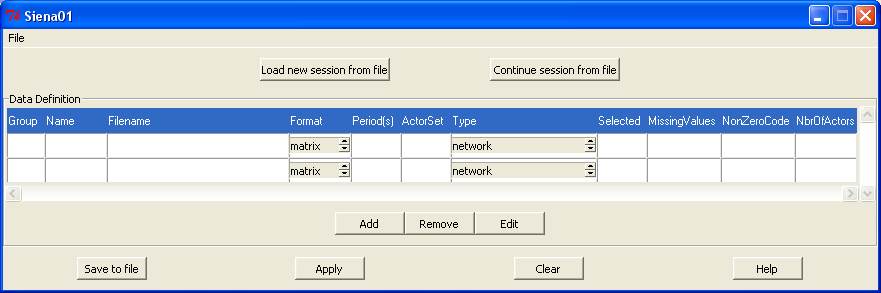
\includegraphics[width=\textwidth]{siena1.png}
\hypertarget{siena1}{}
    \end{center}
\caption{Siena Data Entry Screen}
\label{fig:siena1}
  \end{figure}
\item If the initial screen appears correctly, then check your working directory
  or folder. This is the directory that is opened immediately when clicking the
  \textsf{Add} button.  Various problems can be avoided by making sure that the
  working directory is the directory that also contains the data files and the
  saved session file
  (see below)!\\
  You need to have permission to write files in the working directory, and the
  data files you want to use need to be in the same directory. To change the
  directory:
\begin{enumerate}
\item Right click on the shortcut, and select Properties. (if somehow you don't
  have permission to do this, try copying the shortcut and pasting to create
  another with fewer restrictions. (This may not work in Windows 7: you may need
  to copy it from the visible desktop and then paste it in Windows Explorer in
  your personal Desktop area.))  In the \textsf{Start in:} field type the name
  of the directory in which you wish to work, i.e., a directory in which you can
  both read and write files. Then click OK.

\item To run the examples, put the session file and the data files in
the chosen directory before starting \rs.

\item To use your own data, put that data in the chosen directory before
starting \rs.
\end{enumerate}
\end{enumerate}

\subsubsection{Using the graphical user interface from Mac or Linux}
\begin{enumerate}
\item Install \R (most recent version) as appropriate for your computer.
\item Within \Rn, type\\
  \sfn{install.packages("RSiena")}\\
To use the latest beta version, use\\
 \sfn{install.packages("RSiena", repos="http://R-Forge.R-project.org")}

%  \sfn{install.packages("RSiena", repos="http://www.stats.ox.ac.uk/pub/RWin")}

%\item It is possible that Mac users on `Tiger' will need\\
%  \sfn{install.packages("RSiena", repos="http://www.stats.ox.ac.uk/pub/RWin",
%    type="source")}
\item Navigate to the directory RSiena package, (which you can find from within
  R by running \sfn{system.file(package="RSiena")}) and find a file called
  \sfn{sienascript}.  Run this to produce the Siena GUI screen.(You will
  probably have to change the permissions first (e.g.\ \\ \textsf{chmod u+x
    sienascript})).
\item If you want to use the GUI, you need tcl/tk installed. This is an
  (optional) part of the R installation on Mac. On Linux, you may need to
  install Tcl/tk and the extra Tcl/tk package \sfn{tktable}. On
  Ubuntu Linux, the following commands will do what is
  necessary (perhaps version numbers must be adapted):\protect\footnote{Thanks
  to Michael Schweinberger and Krists Boitmanis for supplying these commands.}
\begin{verbatim}
sudo apt-get install tk8.5
sudo apt-get install libtktable2.9
\end{verbatim}
\end{enumerate}

\subsubsection{Running  the graphical user interface: more details}
\label{S_guiinR}

Originally \RS provided access to the GUI interface direct from Windows. This is
not now possible. This section details some helpful notes about starting \RS
within R\protect\footnote{We are
grateful to Paul Johnson for supplying
these ideas.}.
This is done by starting up \R and working with the following commands.
Note that \R is case-sensitive, so you must use upper and lower
case letters as indicated.

First, set the `working directory' of the \R session
to the same directory that holds the data files;
for example,\\
\sfn{setwd('C:/SienaTest')}

\noindent (Note the forward slash\protect\footnote{You can use backward ones but they
 must be doubled: \sfn{setwd('C:\textbackslash\textbackslash SienaTest')}.},
 and the quotes are necessary\protect{\footnote{Single or double, as long as they match.}.)
Windows users can use the \sfn{Change dir...} option on the \sfn{File} menu.

You can use the following commands to make sure the working directory is
what you intend and see which files are included in it:\\
\sfn{ getwd()}\\
\sfn{ list.files()}

Assuming you see the data files, then you can proceed to load the
\RS package, with the library function:\\
\sfn{ library(RSiena)}\\
The other packages will be loaded as required, but if you wish to examine them
or use other facilities from them you can load them using:\\
\sfn{ library(snow)}\\
\sfn{ library(network)}\\
\sfn{ library(rlecuyer)}\\
The following command
will give a review of
the functions that \RS offers:\\
\sfn{ library(help=RSiena)}\\
After that, you can use the \RS GUI. It will `launch' out
of the \R session.\\
\sfn{ siena01Gui()}\\
You can monitor the \R window for error messages -- sometimes they are
informative.

When you are done, quit \R in the polite way:\\
\sfn{q()} \\(Windows users may quit from the \sfn{File} menu or by closing the
window.)

\subsubsection{Entering Data.}
\label{thegui}
There are two ways to enter the data.
\begin{enumerate}
\item Enter each of your data files using \sfn{Add}.\\
      Fill in the various columns as described in Section~\ref{S_de_screen}.
\item If you have earlier saved the specification
      of data files, e.g., using \sfn{Save to file}, then you can
      use \sfn{Load new session from File}.\\
      This requires a file in the format described
      at the end of  Section~\ref{S_de_screen};
      such a file can be created and read in an editor or spreadsheet program,
      and it is created in .csv (comma separated) format
      by the \sfn{ siena01Gui()} when you request
      \sfn{Save to file}.
\item If you wish to remove files, use the \sfn{Remove} option rather than
  blanking out the entries.
\end{enumerate}
Once you have done this, check that the \sfn{Format},
\sfn{Period}, \sfn{Type}, etc., are correct, and enter any
values which indicate missingness in the \sfn{Missing Values} column.
A (minimal) complete screen is shown in \hyperlink{siena2}
{Figure~\ref{fig:siena2}}.
The details of this screen are explained in Section~\ref{S_de_screen}.
  \begin{figure}[ht]
\hypertarget{siena2}{}
    \begin{center}
      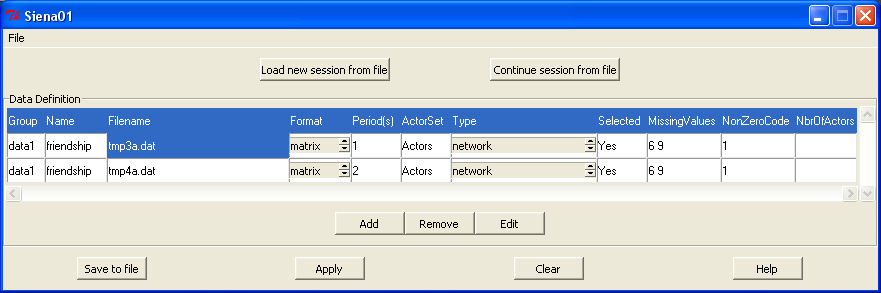
\includegraphics[width=\textwidth]{siena2.png}
    \end{center}
 \caption{Example of a Completed Data Entry Screen}
 \label{fig:siena2}
\end{figure}

\subsubsection{Running the Estimation Program}
\label{estgui}
\begin{enumerate}
\item Click \sfn{Apply}: you will be prompted to save your work. Then you should
  see the \sfn{Model Options} screen shown in \hyperlink{options}{Figure
    \ref{fig:options}}.
  \begin{figure}[ht]
      \hypertarget{options}{}
    \begin{center}
      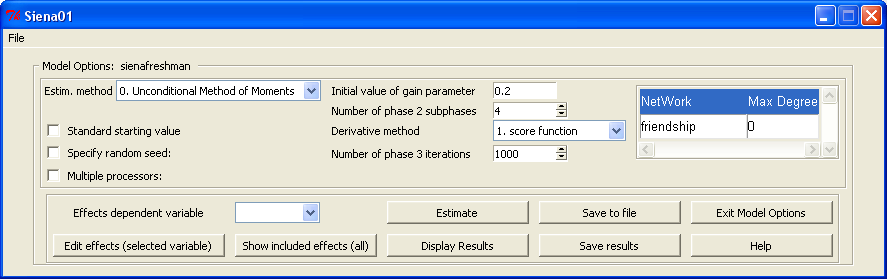
\includegraphics[width=\textwidth]{siena3.png}
    \end{center}
\caption{Model options screen}
\label{fig:options}
  \end{figure}
    If this does not happen, then one possible source of error is that the
    program cannot find your files; e.g.,
    the files are not in the working directory (see above) but in a different
    directory.\\
    If errors occur at this moment and the options screen does not appear,
    then you can obtain diagnostic error messages
    working not through the \sfn{siena01Gui}, but directly  within \R
    as described in Section~\ref{S_slightlyR}.
    This will hopefully help you solving this problem; later on
    you can then work through the \sfn{siena01Gui} again.
\item Select the options you require.
\item Use \sfn{Edit Effects} to choose the effects you wish to include. Note you
  can edit the effects for just one dependent variable at a time if you wish
  by selecting one dependent variable in `Effects dependent variable'.
\item Click \sfn{Estimate}.
\item You should see the \SI screen of the estimation program.
\item When the program has finished, you should see the results. If not, click
  \sfn{Display Results} to see the results.  The output file which you will see
  is stored, with extension \texttt{.out} in the directory in which you start
  \sfn{siena.exe}.
\item You may restart your estimation session at a later date using the
  \sfn{Continue session from file} on the \sfn{Data Entry Screen}.\\
  The restart needs a saved version of the data, effects and model as R
  objects. This will be created automatically when you first enter the
  \sfn{Model Options Screen}, using the default effects and model. You may save
  the current version at any time using the \sfn{Save to file} button, and will
  be prompted to do so when you leave this screen.
\end{enumerate}

\subsubsection{Details of The Data Entry Screen}
\label{S_de_screen}

\begin{description}
\item[\sfn{Group}] May be left blank unless you wish to use the
  \sfn{multi-group} option described in Section~\ref{S_multigroup}. Should not
  contain embedded blanks.
\item[\sfn{Name}] Network files or dyadic covariates should use the same name
  for each file of the set. Other files should have unique names, a list of
  space separated ones for constant covariates.
\item[\sfn{File Name}] Usually entered by using a file selection box, after
  clicking \sfn{Add}.
\item[\sfn{Format}] Only relevant for networks or dyadic covariates. Can be
  a matrix; a single
  Pajek network (\sfn{.net}) (not for two-mode networks);
  or a \sfn{Siena network file} (an edgelist,
  containing three or four columns: (from, to, value, wave (optional)), not yet
  tested for dyadic covariates!).
  By specifying the waves in the fourth column in the \sfn{Siena} format,
  one file can be used to contain data for all the waves.
%(\sfn{.paj} file support will be added
  %later, with a specific button to load a complete project.)
\item[\sfn{Period(s)}] Only relevant for networks and dyadic covariates. All
  other files cover all the relevant periods. Indicates the order of the network
  and dyadic covariate files. Should range from 1 to \sfn{M} within each
  \sfn{group}, where \sfn{M} is the number of time points (waves).
  Use multiple numbers separated by spaces for multi-wave Siena
  network files.
\item[\sfn{ActorSet}] If you have more than one set of nodes, use this column to
  indicate which is relevant to each file. Should not contain embedded blanks.
\item[\sfn{Type}] Indicate here what type of data the file contains. Options
  are:
\begin{description}
\item[\sfn{network}] (i.e., a one-mode network)
\item[\sfn{bipartite}] (i.e., a two-mode network)
\item[\sfn{behavior}]
\item[\sfn{constant covariate}]
\item[\sfn{changing covariate}]
\item[\sfn{constant dyadic covariate}]
\item[\sfn{changing dyadic covariate}]
\item[\sfn{exogenous event}] (for changing composition of the actor set)
\end{description}
\item[\sfn{Selected}] Yes or No. Files with \sfn{Yes} \emph{or blank} will be
included in the model. Use this field to remove any networks or behavior
variables that are not required in the model.
\item[\sfn{Missing Values}] Enter any values which indicate missingness, with
  spaces between different entries.
\item[\sfn{Nonzero Codes}] Enter any values which indicate ties, with spaces
  between different entries.
\item[\sfn{NbrOfActors}] For \sfn{Siena network files}, enter the number of
  actors. For \sfn{Siena net bipartite files}, enter the two dimensions
  (number of rows, number of columns) of the network, separated by a blank space.
 \end{description}

 The details of the screen can be saved to a \emph{session} file, from which
 they can be reloaded. But you can create a session file directly: it should
 have columns with exactly the same names and in exactly the same order as those
 of the \sfn{Data Entry} screen, and be of any of the following types:
\begin{center}
\begin{tabular}{lll}\\
Extension&Type\\
\texttt{.csv}&Comma separated\\
\texttt{.dat} or \texttt{.prn}&Space delimited\\
\texttt{.txt}&Tab delimited\\
\end{tabular}
\end{center}

\noindent
The root name of this input file will also be the root name of the output file.

\subsubsection{Continuing the estimation}
\begin{enumerate}
\item Below you will see some points about how to evaluate the reliability of
  the results.  If the convergence of the algorithm is not quite satisfactory
  but not extremely poor, then you can continue just by \textsf{Apply}ing the
  estimation algorithm again.
\item If the parameter estimates obtained are very poor (not in a reasonable
  range), then it usually is best to start again, with a simpler model, and from
  a standardized starting value.  The latter option must be selected in the
  \textsf{Model Options} screen.
\end{enumerate}


\subsection{Using \SI within \Rn}
\label{S_SR}

There are two alternatives, depending on your familiarity with \Rn,
treated in Sections~\ref{S_slightlyR} and~\ref{S_fullyR}.
Section~\ref{S_guiToR} explains how to make the step from the use of the
GUI to the use of \R commands in the regular \R way.

Section \ref{S_Rscript} presents an example of an \R script
for getting started with \rs.

\smallskip

\subsubsection{For those who are slightly familiar with \Rn}
\label{S_slightlyR}

\begin{enumerate}
\item Install \Rn.
\item Install (within \Rn) the package \rs, and
  possibly \sfn{network} (required to read Pajek files), \sfn{snow} and
  \sfn{rlecuyer} (required to use multiple processes).
\item Set the working directory of \R appropriately (\sfn{setwd()} within \Rn
 or via a desktop shortcut).
\item You can get help by the command
\begin{verbatim}
help(RSiena)
\end{verbatim}
      This will open a browser window with help information;
      by clicking on the `Index' link in the bottom line of this window,
      you get a window with all  \RS commands.\\
      The command
\begin{verbatim}
RShowDoc("RSiena_Manual", package="RSiena")
\end{verbatim}
      opens the official \RS manual.
\item Create a session file using \sfn{siena01Gui()} within \Rn, or using an
  external program.
\item Then, within \Rn,
\begin{enumerate}
\item Use \sfn{sienaDataCreateFromSession()} to create your data objects.
\item Use \sfn{getEffects()} to create an effects object.
\item Use \sfn{fix()} to edit the effects object and select the required
  effects, by altering the \sfn{Include} column to \sfn{TRUE}.
\item Use \sfn{sienaModelCreate()} to create a model object.
\item Use \sfn{siena07()} to run the estimation procedure.
\end{enumerate}
Basic output will be written to a file. Further output can be obtained by using
the\\ \sfn{verbose=TRUE} option of \sfn{siena07}.
\end{enumerate}

\subsubsection{For those fully conversant with \Rn}
\label{S_fullyR}

\begin{enumerate}
\item Add the package \RS
\item Get your network data (including dyadic covariates)
   into matrices, or sparse matrices of type
  \sfn{dgTMatrix}. \sfn{spMatrix()} (in package \sfn{Matrix}) is useful to
  create the latter.
\item Covariate data should be in vectors or matrices.
\item All missing data should be set to NA.
\item Create \SI objects for each network, behavior variable and covariate,
  using the functions \sfn{sienaNet()} (for both networks and behavior
  variables), \sfn{coCovar()} etc.
\item Create a \SI data object using \sfn{SienaDataCreate()}.
\item Use \sfn{getEffects()} to create an effects object.
\item Use functions such as \sfn{includeEffects()}, \sfn{setEffect()},
 and \sfn{includeInteraction()} to further specify the model.
\item Use \sfn{sienaModelCreate()} to create a model object.
\item Use \sfn{siena07()} to run the estimation procedure.
\item Note that it is possible to use multiple processes in \sfn{siena07}. For
  details see section~\ref{S_multipleProcesses}.
\item Also note the availability of the parameter \sfn{prevAns} to reuse
  estimates and derivatives from a previous run with similar effects.
\end{enumerate}
Basic output will be written to a file. Further output can be obtained by using
the \sfn{verbose=TRUE} option of \sfn{siena07}.
The scripts on the scripts page of the \RS website give many examples of
how to use \rs.

\subsubsection{The transition from using the graphical user interface to commands}
\label{S_guiToR}

At some moment, for users who started learning the use of \RS through the GUI,
it can be desirable to make the transition to using commands in the regular \R way.
This will make available more options and integration with other \R features.
The transition can easily be made as follows.

After having made at least one estimation run
in the GUI (which could be with the default
model specification, without having made any further additions to the model;
but it could also be with a more complicated model), click the button
\sfn{Save to file}. You will be prompted for a file name with extension \sfn{.RData}.
Make sure that you do give a non-empty name before the dot in \sfn{.RData};
for the moment, let us choose the name  \sfn{trans.RData}.

Then later in an \R session you can load the  \sfn{trans.RData}.
This can be done in Windows by selecting \sfn{File -- Load Workspace} from the drop down
menu, and entering this file name. It can also be done by entering the command
\begin{verbatim}
load("trans.RData")
\end{verbatim}
This will make available three objects, for data, model, and effects.
What is currently in your workspace is shown by the command
\begin{verbatim}
ls()
\end{verbatim}
This will probably show that the loaded objects have the names
\sfn{mydata}, \sfn{mymodel}, and \sfn{myeff}.
These are the type of objects created by the functions \sfn{sienaDataCreate},
\sfn{sienaModelCreate}, and \sfn{getEffects},
and discussed in the \SI script in Section~\ref{S_Rscript}.

Now attach the package \RS and subsequently ask for the descriptions of these
three objects:
\begin{verbatim}
library(RSiena)
mydata
mymodel
myeff
\end{verbatim}
This will give short descriptions and thereby a confirmation of what has been
imported from the GUI session to the regular \R session.
From here on you can continue and work with \R commands,
as in the script, to further specify the model by working
on the effects object, and then estimate the parameters by the \sfn{siena07}
function.

The precise point to continue from here, using the scripts
in the next section and also on the \RS website,
is to use
script \sfn{RscriptSienaVariableFormat.R},
starting with section~D (\emph{Defining Effects}),
part~3 (\emph{Adding/removing effects using includeEffects}).
After this, you are advised to continue with script
\sfn{RscriptSienaRunModel.R}.


\subsection{An example \R script for getting started}
\label{S_Rscript}

The best way to get acquainted with \RS is perhaps
going through some existing scripts.
The script  below is useful for this purpose.
At the `RSiena scripts' page
\url{http://www.stats.ox.ac.uk/~snijders/siena/siena_scripts.htm}
 of the \RS website
it is available divided into smaller pieces, and updated.
The script is written so as to be useful for novice
as well as experienced \R users.
The `RSiena scripts' page of the \RS website
also contains some other scripts that may be useful.
The appendix of this manual contains a list of \RS functions which may be consulted
in addition to this script.

{\footnotesize
\verbatiminput{RscriptDataFormat.R}
\newpage
\verbatiminput{RscriptSienaVariableFormat.R}
\verbatiminput{RscriptSienaRunModel.R}
\newpage
\verbatiminput{RscriptSienaBehaviour.R}
}

\subsection{Outline of estimation procedure}
\noindent
\SI estimates parameters by the following procedure:
\begin{enumerate}
\item  Certain statistics are chosen that should reflect the parameter values;\\
  the finally obtained parameters should be such that the \emph{expected
    values}
  of the statistics are equal to the \emph{observed values}.\\
  Expected values are approximated as the averages over a lot of simulated
  networks.\\
  Observed values are calculated from the data set. These are also called the
  \emph{target values}.
\item To find these parameter values, an \emph{iterative stochastic simulation
    algorithm}
  is applied.\\
  This works as follows:
\begin{enumerate}
\item In Phase 1, the sensitivity of the statistics to the parameters is roughly
  determined.
\item In Phase 2, provisional parameter values are updated:\\
  this is done by simulating a network according to the provisional parameter
  values, calculating the statistics and the deviations between these simulated
  statistics and the \emph{target values}, and making a little change (the
  `update') in the parameter values
  that hopefully goes into the right direction.\\
  (Only a `hopefully' good update is possible, because the simulated network is
  only a random draw from the distribution of networks, and not the expected
  value itself.)
\item In Phase 3, the final result of Phase 2 is used, and it is checked if the
  average statistics of many simulated networks are indeed close to the target
  values. This is reflected in the so-called \texttt{t statistics for deviations
    from targets}.
\end{enumerate}
\end{enumerate}

\subsection{Using multiple processes}
\label{S_multipleProcesses}
\begin{enumerate}
\item
If multiple processors are available, then using
multiple processes can speed up the estimation in \sfn{siena07}.

\item In Phases 1 and 3 the simulations are performed in parallel. In Phase 2,
  multiple simulations are done with the same parameters, and the resulting
  statistics are averaged. The gain parameter is increased and the
  number of iterations in phase 2 reduced to take advantage of
  the increased accuracy.

\item The parameters required to run all processes on one computer are fairly
  simple: in your call to \sfn{siena07}, set \sfn{nbrNodes} to the number of
  processes and \sfn{useCluster} and \sfn{initC} to TRUE. The \sfn{Model
    Options} screen also allows you to specify the number of processes, and
  will automatically set the other required parameters for you.

\item To use more than one machine is more complicated, but it can be done by
  using, in addition, the \sfn{clusterString} parameter.  The computers need to
  be running incoming \sfn{ssh}.
\item For machines with exactly the same layout of \R
  directories on each, simply set \sfn{clusterString} to a character vector of
  the names of the machines.
\item For other cases, e.g.\ using Macs alongside Linux,
  see the documentation for the package \sfn{snow}.

\item Currently \RS uses sockets for inter-process communication.
\item Each process needs a copy of the data in memory. If there is insufficient
  memory available there will be no speed gain as too much time will be spent
  paging.
\item In each iteration the main process waits until all the other processes
  have finished. The overall speed is therefore that of the slowest process, and
  there should be enough processors to allow them all to run at speed.
\end{enumerate}

\subsection{Steps for looking at results: Executing \si .}
\label{S_exec}

\begin{enumerate}
\item Look at the start of the output file for general data
      description (degrees, etc.), to check your data input.
    \item When parameters have been estimated, first look at the \texttt{t
        ratios for deviations from targets}.  These are good if they are all
      smaller than 0.1 in absolute
      value, and reasonably good if they are all smaller than 0.2.\\
      We say that the algorithm has converged if they are all smaller than 0.1
      in absolute value, and that it has nearly converged if they are all
      smaller than 0.2.\\
      These bounds are indications only, and may be taken with a grain of
      salt.
\item In rare circumstances, when the data set leads to instability
      of the algorithm, the following may be of use.\\
      The \textsf{Initial value of the gain parameter} determines the
      step sizes in the parameter updates in the iterative
      algorithm.
      This is the parameter called \textsf{firstg}
      in function \textsf{sienaModelCreate}.
      A too low value implies that it takes very long to attain a
      reasonable parameter estimate when starting from an initial
      parameter value that is far from the `true' parameter estimate.
      A too high value implies that the algorithm will be unstable,
      and may be thrown off course into a region of unreasonable
      (e.g., hopelessly large) parameter values.\\
      It usually is unnecessary to change
      this.
    \item If all this is of no avail, then the conclusion may be that the model
      specification is incorrect for the given data set.
    \item Further help in interpreting output is in Section~\ref{S_output} of
      this manual.
\end{enumerate}

\subsection{Giving references}

When using \si, it is appreciated that you refer to this manual and to one or
more relevant references of the methods implemented in the program.  The
reference to this manual is the following.  \smallskip

\noindent
Ripley, Ruth M., Snijders, Tom A.B., and Preciado Lopez, P.
2011.
Manual for SIENA version 4.0 (version \today).
Oxford: University of Oxford, Department of Statistics; Nuffield College.
\textsf{http://www.stats.ox.ac.uk/siena/}

\smallskip

A basic reference for the network dynamics model is \citet{Snijders01}
or \citet{Snijders05}.
Basic references for the model of network-behavior co-evolution
are \citet*{SnijdersEA07} and \citet*{SteglichEA10}.
A basic reference for the Bayesian estimation is \citet{KoskinenSnijders07}
and for the maximum likelihood estimation \citet*{SnijdersEA10a}.

More specific references are \citet{Schweinberger10} for the score-type goodness
of fit tests and \citet{SchweinbergerSnijders07a} for the calculation of
standard errors of the Method of Moments estimators. For assessing and
correcting time heterogeneity, and associated model selection considerations,
refer to \citet*{Lospinoso2011}.

A tutorial is \citet*{SnijdersEA10b}.


\subsection{Getting help with problems}
\label{sec:problems}
If you have a problem running \rs, please read through the following hints to
see if any of them help. If not, please send an email to
rsiena-help@lists.r-forge.r-project.org, or post in the help forum for \RS in
R-forge. You need to be a registered member of R-forge (and possibly of \rs)
to post to a forum, but anyone can send emails (at present!). In your message,
please tell us which operating system , which version of \Rn, and which version
of \RS you are using.

For queries about the modelling aspects of \si, or interpretation, please
continue to use the \SN/ \RS mailing list.


\begin{description}
\item[Check your version of \RS] Details of the latest version available can
  be found at \url{http://r-forge.r-project.org/R/?group_id=461}. The version is
  identified by a version number (e.g.\ 1.0.9) and an R-forge revision
  number. You can find both the numbers of your current installed version by
  opening \R, and typing \\
  \verb|packageDescription("RSiena")|. The version is
  near the top, the revision number near the end. Both are also displayed at the
  start of \SI output files (use \sfn{print01Report} to get the relevant output
  file if you are not using the GUI.)
\item[Check your version of \Rn] When there is a new version or revision of \RS
  it will only be available to you automatically if you are running the most
  recent major version of \Rn. (You can force an installation if
  necessary by downloading the tarball or binary and installing from that, but
  it is better to update your \Rn.)
\item [Check both repositories] We have two repositories in use for \rs: CRAN
  and R-forge. The latest version will always be available from
  R-forge. (Frequent updates are discouraged on CRAN, so bug-fixes are likely to
  appear first on R-forge.)
\item[Installation] When using the repository at R-forge, \emph{install} the
  package rather than updating it. Then check the version and revision numbers.
\end{description}


\newpage

%\addtocontents{toc}{\vspace{-2ex}}  % hack to avoid a 3-page table of contents

\part{Users' manual}

\section[Program parts]{Parts of the program}
\label{S_parts}

The operation of the \SI program is comprised of five main parts:
\begin{enumerate}
 \item input of basic data description,
 \item model specification,
 \item estimation of parameter values using stochastic simulation,
 \item testing parameters and assessing goodness of fit,
 \item simulation of the model with given and fixed parameter values.
\end{enumerate}

The normal operation is to start with data input, then specify a
model and estimate its parameters,
assess goodness of fit and the significance of the parameters,
and then possibly continue with new
model specifications followed by estimation or simulation.

The main output is written to a text file named
\textsf{\textsl{pname}.out}, where \textsf{\textsl{pname}} is the name
specified in the call of \textsf{sienaModelCreate()}.

\newpage

\section{Input data}
\label{S_InputData}

\SI  is a program for the statistical analysis
of repeated measures of social networks, and requires network data
collected at two or more time points. It is possible to include
changing actor variables (representing behavior, attitudes,
outcomes, etc.) which also develop in a dynamic process, together
with the social networks.
As repeated measures data on social networks, at the very least, {\em two or more data
files with digraphs} are required: the observed networks, one for
each time point. The number of time points is denoted $M$.

In addition, various kinds of variables are allowed:

\begin{enumerate}
\item {\em actor-bound} or {\em individual variables},
      also called {\em actor attributes},
      which can be symbolized as $v_i$ for each actor $i$;
      these can be constant over time or changing; \\
      the changing individual variables can be dependent variables
      (changing dynamically in mutual dependence with the changing network;
      then they are also called dependent behavior variables)
      or independent variables (exogenously changing variables;
      then they are also called individual covariates).
\item {\em dyadic covariates}, which can be symbolized as $w_{ij}$
      for each ordered pair of actors $(i,j)$;
%they are allowed only
%      to have integer values ranging from 0 to 255.
%      If one has real-valued dyadic covariates, then one option
%      is to multiply them e.g. by 10 or 100 so that they still have a range
%      between 0 and 255, and used the rounded values.
     these likewise can be constant over time or changing.
\end{enumerate}

Dependent variables (which can be networks or behavior variables)
all must be available for the same set of time points.

All variables must be available in ASCII (`raw text') data files, described in
detail below. It is best to use the `classical' type of filenames, without embedded blanks
and not containing special characters.
These files, the names of the corresponding
variables, and the coding of missing data, must be made available
to \si.

Names of variables must be composed of at most 12 characters. This
is because they are used as parts of the names of effects which
can be included in the model, and the effect names should not be
too long.

\subsection{Digraph data files}

Each digraph must be contained in a separate input file.
For data specification by the \textsf{sienaNet} function, the network
must be specified as a matrix.
For data specification by the graphical interface \textsf{siena01Gui}
or by the function \textsf{sienaDataCreateFromSession},
edge list formats are also allowed. This can be either the
format of the Pajek program, or a raw edge list, here called Siena format.
For large number of nodes (say, larger than 100), the edge list
format is more efficient in use of computer memory.
Data input as edge lists will also be made available by means of the
\textsf{sienaNet} function (in some future version of \sn).
\begin{enumerate}
\item \emph{Adjacency matrices}.\\
      The first is an adjacency matrix, i.e., $n$ lines each with $n$ integer
      numbers, separated by blanks or tabs, each line ended by a hard return.
      The diagonal values are meaningless but must be present.

      Although this section talks only about digraphs (directed graphs), it is
      also possible that all observed adjacency matrices are symmetric.
      This will be automatically detected by \si, and
      the program will then utilize methods for non-directed networks.

      The data matrices for the digraphs
       must be coded in the sense
      that their values are converted by the program to the 0 and 1
      entries in the adjacency matrix. A set of code numbers is required
      for each digraph data matrix; these codes are regarded as the
      numbers representing a present arc in the digraph, i.e., a 1 entry
      in the adjacency matrix; all other numbers will be regarded as 0
      entries in the adjacency matrix. Of course, there must be at least
      one such code number. All code numbers must be in the range from 0
      to 9, except for structurally determined values (see below).

      This implies that if the data are already in 0-1 format, the
      single code number 1 must be given. As another example, if the
      data matrix contains values 1 to 5 and only the values 4 and 5 are
      to be interpreted as present arcs, then the code numbers 4 and 5
      must be given.
    \item \emph{Pajek format}.\\
      If the digraph data file has extension name \texttt{.net}, then the
      program assumes that the data file has Pajek format.  The format required
      differs from that in the previous versions of \SI.  The file should relate
      to one observation only, and should contain a list of vertices (using the
      keyword \texttt{*Vertices}, together with (currently) a list of arcs,
      using the keyword \texttt{*Arcs}
      followed by data lines according to the Pajek rules.
      These keywords must be in lines that contain no further characters.
      An example of such input files is given in the s50 data set
      that is distributed in the \texttt{examples} directory.
    \item \emph{Siena format}.\\
      An edge list containing three or four columns:
      from, to, value, wave (optional).\\
      Like the Pajek format, this has the advantage that absent ties
      (tie variables with the value 0) do not need to be mentioned
      in the data file.
      By specifying the waves in the fourth column in the \sfn{Siena} format,
      one file can be used to contain data for all the waves.
\end{enumerate}

Missing values must be indicated in the way usual for \Rn,
by \texttt{NA}.
For data specification by the graphical interface \textsf{siena01Gui}
or by the function \textsf{sienaDataCreateFromSession},
instead of \texttt{NA} any numerical code can be used
given that this is indicated to be a missing value code.

Although this section talks only about digraphs (directed graphs), it is
also possible that all observed ties (for all time points) are mutual.
This will be automatically detected by \si, and
the program will then utilize methods for non-directed networks.

If the data set is such that it is never observed that ties are terminated,
then the network dynamics is automatically specified internally in such a way
that termination of ties is impossible.
(In other words, in the simulations of the actor-based model
the actors have only the option to create new ties or to retain
the status quo, not to delete existing ties.)
Similarly if ties never are created (but only terminated),
then this will be respected in the simulations.

\subsubsection{Transformation between matrix and edge list formats}

The following \R commands can be used for transforming an
adjacency matrix to an edge list, and back again.
If \texttt{a} is an adjacency matrix, then the following commands
can be used to create the corresponding edge list,
called \texttt{edges} here.
 \begin{verbatim}
 # create indicator matrix of non-zero entries of a
 ones <- !a %in%  0
 # create empty edge list of desired length
 edges <- matrix(0, sum(ones), 3)
 # fill the columns of the edge list
 edges[, 1] <- row(a)[ones]
 edges[, 2] <- col(a)[ones]
 edges[, 3] <- a[ones]
 # if desired, order edge list by senders and then receivers
 edges      <- edges[order(edges[, 1], edges[, 2]), ]
 \end{verbatim}
Some notes on the commands used here:\\
These commands can be used not only if the adjacency matrix
contains only 0 and 1 entries, but also if it contains values
\texttt{NA}, 10, or 11. The possibility of \texttt{NA}
entries requires special attention;
\texttt{\%in\%}
does just what we need, as it quietly says that
\texttt{NA}'s are not \texttt{\%in\%}
anything, returning \texttt{FALSE}, which is transformed to
\texttt{TRUE} by the \texttt{!} function.
The edge list is created having all 0 values and at the end
should have no 0 values at all.

It is more efficient, however, to work with sparse matrices;
this also is done internally in \rs.
Using the \texttt{Matrix} package for sparse matrix manipulations,
the same results can be obtained as follows.
\begin{verbatim}
library(Matrix)
tmp <- as(Matrix(a), "dgTMatrix")
edges2 <- cbind(tmp@i + 1, tmp@j + 1, tmp@x)
\end{verbatim}
Conversely, if \texttt{edges} is an edge list, then the following commands
can be used to create the corresponding
adjacency matrix, called \texttt{adj},
with $n$ nodes. (For a bipartite network the two dimensions
will normally be distinct numbers.)
\begin{verbatim}
# create empty adjacency matrix
adj <- matrix(0, n, n)
# put edge values in desired places
adj[edges[, 1:2]] <- edges[, 3]
\end{verbatim}
Note that this starts with a matrix having all 0 entries,
and results in a matrix with no 0 entries at all.
To check the results, after doing these two operations, the command
\begin{verbatim}
length(which(a != adj))
\end{verbatim}
should return the value 0.

Note that the basic edge list, \verb|edges|, lacks information as to the size of
the adjacency matrix. \verb|tmp| above is a sparse matrix which is in edge list
format but includes information on the size of the adjacency matrix, and can be
used in a similar way to the original matrix \verb|a| while saving memory space.

\subsubsection{Structurally determined values}
\label{S_struct}

It is allowed that some of the values in the digraph are
structurally determined, i.e., deterministic rather than random.
This is analogous to the phenomenon of `structural zeros' in
contingency tables, but in \SI not only structural zeros but also
structural ones are allowed. A structural zero means that it is
certain that there is no tie from actor $i$ to actor $j$; a
structural one means that it is certain that there is a tie. This
can be, e.g., because the tie is impossible or formally imposed,
respectively.

Structural zeros provide an easy way to deal with actors leaving
or joining the network between the start and the end
of the observations. Another way
(more complicated but it gives possibilities to represent actors
entering or leaving at specified moments between observations)
is described in Section~\ref{S_comp}.

Structurally determined values are defined by reserved codes in
the input data: the value 10 indicates a structural zero, the
value 11 indicates a structural one. Structurally determined
values can be different for the different time points. (The
diagonal of the data matrix always is composed of structural
zeros, but this does not have to be indicated in the data matrix
by special codes.) The correct definition of the structurally
determined values can be checked from the brief report of this in
the output file.
%, and by looking at the file \textsf{\em pname}.s01
%(for the first time point), \textsf{\em pname}.s02 (second time
%point), etc. In these files, the structurally determined positions
%(structural zeros as well as structural ones) are indicated by the
%value 1, all others (i.e., the positions where ties are random) by
%the value 0.

Structural zeros offer the possibility of analyzing several
networks simultaneously under the assumption that the parameters
are identical.
Another option to do this is given in Section~\ref{S_mulev}.
E.g., if there are three networks with 12, 20 and
15 actors, respectively, then these can be integrated into one
network of 12 + 20 + 15 = 47 actors, by specifying that ties
between actors in different networks are structurally impossible.
This means that the three adjacency matrices are combined in one
$47 \times 47$ data file, with values 10 for all entries that
refer to the tie from an actor in one network to an actor in a
different network. In other words, the adjacency matrices will be
composed of three diagonal blocks, and the off-diagonal blocks
will have all entries equal to 10. In this example, the number of
actors per network (12 to 20) is rather small to obtain good
parameter estimates, but if the additional assumption of identical
parameter values for the three networks is reasonable, then the
combined analysis may give good estimates.

In such a case where $K$ networks (in the preceding paragraph, the
example had $K = 3$) are combined artificially into one bigger
network, it will often be helpful to define $K-1$ dummy variables
at the actor level to distinguish between the $K$ components.
These dummy variables can be given effects in the rate function
and in the evaluation function (for ``ego"), which then will
represent that the rate of change and the out-degree effect are
different between the components, while all other parameters are
the same.

It will be automatically discovered by \SI when functions
depend only on these components defined by structural zeros,
between which tie values are not allowed.
For such variables, only the ego effects are defined
and not the other effects defined for the regular
actor covariates and described in Section ~\ref{S_eff_cov}.
This is because the other effects then are meaningless.
If at least one case is missing (i.e., has the missing value data code
for this covariate),
then the other covariate effects are made available.

When \SI simulates networks including some structurally determined values,
if these values are constant across all observations then
the simulated tie values are likewise constant.
If the structural fixation varies over time, the situation
is more complicated.
Consider the case of two consecutive observations
$m$ and $m+1$,
and let $X^{\text{sim}}_{ij}$ be the simulated value
at the end of the period from $t_m$ to $t_{m+1}$.
If the tie variable $X_{ij}$ is structurally fixed at time $t_m$
at a value $x_{ij}(t_m)$,
then $X^{\text{sim}}_{ij}$ also is equal to $x_{ij}(t_m)$,
independently of whether this tie variable is structurally fixed
at time $t_{m+1}$ at the same or a different value or not at all.
This is the direct consequence of the structural fixation.
On the other hand, the following rule is also used.
If $X_{ij}$ is \emph{not} structurally fixed at time $t_m$
but it is structurally fixed at time $t_{m+1}$ at some value $x_{ij}(t_{m+1})$,
then in the course of the simulation process from  $t_m$ to $t_{m+1}$
this tie variable can be changed as part of the process in the usual way,
but after the simulation is over and before the statistics are calculated it will be fixed
to the value $x_{ij}(t_{m+1})$.

The target values for the algorithm of the Method of Moments estimation
procedure are calculated for all observed digraphs $x(t_{m+1})$.
However, for tie variables $X_{ij}$ that are
structurally fixed at time $t_m$, the observed value  $x_{ij}(t_{m+1})$
is replaced by the structurally fixed value  $x_{ij}(t_{m})$.
This gives the best possible correspondence between target values
and simulated values in the case of changing structural fixation.

\subsection{Dyadic covariates}

As the digraph data, also each measurement of a dyadic covariate
must be contained in a separate input file with a square data
matrix, i.e., $n$ lines each with $n$ integer numbers, separated by
blanks or tabs, each line ended by a hard return. The diagonal values are
meaningless but must be present.
Pajek input format is currently not possible for dyadic covariates.

A distinction is made between constant and changing dyadic
covariates, where change refers to changes over time. Each constant
covariate has one value for each pair of actors, which is valid for
all observation moments, and has the role of an independent
variable. Changing covariates, on the other hand, have one such
value for each period between measurement points. If there are $M$
waves (i.e., observation moments) of network data,
this covers $M-1$ periods, and accordingly,
for specifying a single changing dyadic covariate, $M-1$ data files
with covariate matrices are needed.

% The reasons for restricting dyadic covariates to integer values from
% 0 to 255 are historical and have to do with how the constant dyadic
% covariate data are stored internally. If the user wishes to use a
% dyadic covariate with a different range, this variable first must be
% transformed to integer values from 0 to 255. E.g., for a continuous
% variable ranging from 0 to 1, the most convenient way probably is to
% multiply by 100 (so the range becomes 0--100) and round to integer
% values.

The mean is always subtracted from the covariates.
See the section on \hyperlink{T_S_centering}{\emph{Centering}}.

\subsection{Individual covariates}

Individual (i.e., actor-bound) variables can be combined in one or
more files. If there are $k$ variables in one file, then this data
file must contain $n$ lines, with on each line $k$ numbers which all
are read as real numbers (i.e., a decimal point is allowed). The
numbers in the file must be separated by blanks and each line must
be ended by a hard return. There must not be blank lines after the
last data line.

Also here, a distinction is made between constant and changing actor
variables. Each constant actor covariate has one value per actor
valid for all observation moments, and has the role of an
independent variable.

Changing variables can change between observation moments. They
can have the role of dependent variables (changing dynamically in
mutual dependence with the changing network) or of independent
variables; in the latter case, they are also called `changing
individual covariates'. Dependent variables are treated in the
section below, this section is about individual variables
in the role of independent variables -- then they are also
called individual covariates.

When changing individual variables have the role of
independent variables, they are assumed to have constant values from one
observation moment to the next. If observation moments for the
network are $t_1, t_2, ..., t_M$, then the changing covariates
should refer to the $M-1$ moments $t_1$ through $t_{M-1}\,$, and
the $m$-th value of the changing covariates is assumed to be valid
for the period from moment $t_m$ to moment $t_{m+1}\,$.
The value at $t_M$, the last moment, does not play a role.
Changing covariates, as independent variables, are meaningful
only if there are 3 or more observation moments,
because for 2 observation moments the distinction between
constant and changing covariates is not meaningful.

Each changing individual covariate must be given in one file,
containing $k = M-1$ columns that correspond to the $M-1$ periods
between observations.
It is not a problem if there is an $M$'th column in the file,
but it will not be read.

The mean is always subtracted from the covariates.
See the section on \hyperlink{T_S_centering}{\emph{Centering}}.

When an actor covariate is constant within waves, i.e.,
within each wave it has the same value for all actors;
or, more generally, when within each wave it has the same value for
all actors
within components separated by structural zeros (which means that
ties between such components are not allowed), then only the ego effect
of the actor covariate is made available.
This is because the other effects then are meaningless.
This may cause problems for combining several data sets
in a meta-analysis (see Section ~\ref{S_mulev}).
If at least one case is missing (i.e., has the missing value data code),
then the other covariate effects are made available.
When analysing multiple data sets in parallel,
for which the same set of effects is desired to be included % in
%the .MO file,
it is therefore advisable to give data sets in which
a given covariate has the same value for all actors
one missing value in this covariate;
purely to make
the total list of effects % in the MO file
independent of the observed data.


\subsection{Interactions and dyadic transformations of covariates}

For actor covariates, two kinds of transformations to dyadic covariates
are made internally in \si. Denote the actor covariate by $v_i$,
and the two actors in the dyad by $i$ and $j$.
Suppose that the range of $v_i$ (i.e., the difference between the
highest and the lowest values) is given by $r_V$.
The two transformations are the following:
\begin{enumerate}
\item \emph{dyadic similarity}, defined by $ 1 - \big( \vert v_i - v_j \vert / r_V \big) $,
      and centered so the the mean of this similarity variable becomes 0;\\
      note that before centering, the similarity variable is 1 if
      the two actors have the same value, and 0 if one has the highest and the
      other the lowest possible value;
\item \emph{same $V$}, defined by 1 if $v_i = v_j$,
      and 0 otherwise (not centered) ($V$ is the name of the variable).
      This can also be referred to as \emph{dyadic identity} with respect to $V$.
\end{enumerate}
Dyadic similarity is relevant for variables that can be treated as interval-level
variables; dyadic identity is relevant for categorical variables.


In addition, \SI offers the possibility of user-defined two- and three-variable
interactions between covariates; see Section~\ref{S_int_eff}.


\subsection{Dependent action variables}
\label{S_depaction}

\SI also allows dependent action variables,
also called dependent behavior variables. This can be used in studies
of the co-evolution of networks and behavior, as described
in \citet*{SnijdersEA07} and \citet*{SteglichEA10}.
These action variables represent the actors' behavior, attitudes, beliefs, etc.
The difference between dependent action variables and changing actor
covariates is that the latter change exogenously, i.e., according
to mechanisms not included in the model, while the dependent
action variables change endogenously, i.e.,
depending on their own values and on the changing network.
In the current implementation only one dependent network variable is
allowed, but the number of dependent action variable can be larger than one.
Unlike the changing individual covariates,
the values of dependent action variables are not assumed to be
constant between observations.

Dependent action variables must have nonnegative integer values;
e.g., 0 and 1, or a range of integers like 0,1,2 or 1,2,3,4,5.
Each dependent action variable must be given in one
file, containing $k = M$ columns, corresponding to the $M$
observation moments.

If any values are not integers, a warning will be printed on the initial report
and the values will be truncated towards zero.


\subsection{Missing data}

\SI allows that there are some missing data on network variables,
on covariates, and on dependent action
variables. Missing data in changing dyadic covariates are not yet
implemented. Missing data must be indicated by missing data codes,
{\em not} by blanks in the data set.

Missingness of data is treated as non-informative.
One should be aware that having many missing data can seriously
impair the analyses: technically, because estimation will be
less stable; substantively, because the assumption of
non-informative missingness often is not quite justified.
Up to $10\%$ missing data will usually not give many difficulties
or distortions, provided missingness is indeed non-informative
\citep{HuismanSteglich08}.
When one has more than $20\%$ missing data on any variable, however,
one may expect problems in getting good estimates.

In the current implementation of \si, missing data are treated in
a simple way, trying to minimize their influence on the estimation
results.
%This method is further explained in \citet{HuismanSteglich08},
%where comparisons are also made with other ways of dealings with the missing
%information.

The basic idea is the following.
\medskip

NOTE: This may not be a correct representation. To be modified.
\medskip

A brief sketch of the procedure is that
missing values are imputed to allow meaningful simulations;
for the calculation of the target statistics in the Method of Moments,
tie variables and actor variables with missings are not
used.
More in detail, the procedure is as follows.

The simulations are carried out over all variables,
as if they were complete.
To enable this, missing data are imputed.
In the initial observation, missing entries in the adjacency
matrix are set to 0,
i.e., it is assumed that there is \emph{no} tie;
this is done because normally data are sparse, so `no tie'
is the modal value of the tie variable.
In the further observations, for any variable,
if there is an earlier observed value of this variable then
the last observed value is used to impute the current
value (the `last observation carry forward' option,
cf.\ \citet{Lepkowski89}); if there is no earlier observed
value, the value 0 is imputed.
For the dependent behavior variables the same principle
is used: if there is a previous observation of the same variable
then this value is imputed, if there is none then the
observationwise mode of the variable is imputed.
Missing covariate data are replaced by the
variable's average score at this observation moment. In the course
of the simulations, however, the adjusted values of the dependent
action variables and of the network variables are allowed to
change.

In order to ensure a minimal impact of missing data treatment on
the results of parameter estimation (method of moments estimation)
and/or simulation runs, the calculation of the target statistics
used for these procedures uses only non-missing data. When
for an actor in a given period, any variable is missing that is
required for calculating a contribution to such a statistic, this
actor in this period does not contribute to the statistic in
question. For network and dependent action variables, the tie variable
or the actor variable, respectively,
must provide valid data both at the beginning and at the end of a
period for being counted in the respective target statistics.

\subsection{Composition change}
\label{S_comp}

\SI can also be used to analyze networks of which the composition
changes over time, because actors join or leave the network
between the observations.
This can be done in two ways: using the method of \citet{HuismanSnijders03},
or using structural zeros.
(For the maximum likelihood estimation option, the Huisman-Snijders method
is not implemented, and only the structural zeros method can be used.)
Structural zeros can specified for all elements of the tie variables
toward and from actors who are absent at a given observation moment.
How to do this is described in subsection~\ref{S_struct}.
This is straightforward and not further explained here.
This subsection explains the method of Huisman and Snijders
(2003), which uses the information about composition change
in a sightly more efficient way.

For this case, a data file is needed in which the
\emph{times of composition change} are given. For networks with
constant composition (no entering or leaving actors), this file is
omitted and the current subsection can be disregarded.

Network composition change, due to actors joining or leaving the
network, is handled separately from the treatment of missing data.
The digraph data files must contain all actors who are part of the
network at any observation time (denoted by $n$) and each actor
must be given a separate (and fixed) line in these files, even for
observation times where the actor is not a part of the network
(e.g., when the actor did not yet join or the actor already left
the network). In other words, the adjacency matrix for each
observation time has dimensions $n \times n$.

At these times, where the actor is not in the network, the entries
of the adjacency matrix can be specified in two ways. First as
missing values using missing value code(s). In the estimation
procedure, these missing values of the joiners before they joined
the network are regarded as 0 entries, and the missing entries of
the leavers after they left the network are fixed at the last
observed values. This is different from the regular missing data
treatment. Note that in the initial data description the missing
values of the joiners and leavers are treated as regular missing
observations. This will increase the fractions of missing data and
influence the initial values of the density parameter.

A second way is by giving the entries a regular observed code,
representing the absence or presence of an arc in the digraph (as
if the actor was a part of the network). In this case, additional
information on relations between joiners and other actors in the
network before joining, or leavers and other actors after leaving
can be used if available. Note that this second option of
specifying entries always supersedes the first specification: if a
valid code number is specified this will always be used.

For joiners and leavers, crucial information is contained in the
times they join or leave the network (i.e., the times of
composition change), which must be presented in a separate input
file, the \emph{exogenous events file}
described in Section~\ref{S_datform}.


\subsection{Centering}

Individual as well as dyadic covariates are
\hypertarget{T_S_centering}{centered}
by the program in the following way.

For individual covariates, the mean value is subtracted
immediately after reading the variables. For the changing
covariates, this is the global mean (averaged over all periods).
The values of these subtracted means are reported in the output.

For the dyadic covariates and the similarity variables derived
from the individual covariates, the grand mean is calculated,
stored, and subtracted during the program calculations. (Thus,
dyadic covariates are treated internally by the program differently than
individual covariates in the sense that the mean is subtracted at
a different moment, but the effect is exactly the same.)
Unlike the `covariate similarity' effect,
the `same covariate' effect is not centered but keeps its 0-1 values.

The formula for balance is a kind of dissimilarity between rows of
the adjacency matrix. The mean dissimilarity is subtracted in this
formula and also reported in the output. This mean dissimilarity
is calculated by a
\hyperlink{T_meanbal}{formula given in Section}~\ref{S_math}.

%The dependent network variable is not centered.

\subsection{Monotone dependent variables}

In some data sets, a dependent variable only increases, or only decreases.
For a network, this means that ties can be created but not terminated,
or the other way around.
This may be the case for all periods (a period is defined by the
two consecutive observation waves at its start and end points)
or just in some of the periods.
\RS will note when a dependent variable only increases or only decreases,
and mention this in the output file generated by \textsf{print01Report}.
This constraint then is also respected in the simulations, in the periods
where it is observed.
This is represented
internally by a variable called \texttt{uponly} indicating that the
dependent variable cannot decrease,
and a variable \texttt{downonly} indicating that the
dependent variable cannot increase.

If a dependent variable is only increasing or only decreasing
for all periods, then two of the basic effects defined below
are not identified.
These are the outdegree effect for a dependent network variable,
and the linear shape effect for a dependent behavior variable;
these effects define the balance between the probabilities of
going up and going down.
These effects then are dropped automatically from the effects object,


\newpage
\section{Model specification}
\label{S_modspec}

\subsection{Definition of the model}
\label{S_defmod}

After defining the data, the next step is to specify a model.
The model specification consists of a selection of `effects'
for the evolution of each dependent variable (network or behavior).
To understand this, first a brief review of the definition of the
actor-oriented model is given
\citep*[for further explanations see][]{Snijders01, Snijders05,
SnijdersEA07, SnijdersEA10b}.

The model is based on four functions, which first are explained in an
intuitive way.
These functions depend on the actor (hence the name `actor-oriented')
and on the state of the network, behavior, and covariates.
All these functions are constituted by a weighted sum
of so-called \emph{effects}, which define the characteristics of
the network (and behavior, if this is included as a dependent variable)
that determine the probabilities of changes.


\begin{itemize}
\item \emph{rate function}\\
The rate function models the speed by which the dependent variable
changes; more precisely: the speed by which each network actor
gets an opportunity for changing her score on the dependent
variable.\\
Advice: in most cases, start modeling with a constant rate function without
additional rate function effects.
(When there are important size or activity differences between
actors, it is possible that different advice must be given,
and it may be necessary to let the rate function
depend on the individual covariate that indicates this size;
or on the out-degree.)
\item {\em evaluation function }\\
The evaluation function\footnote{The evaluation function was called
\emph{objective function} in \citet{Snijders01}.}
is the primary determinant of the probabilities of changes.
Probabilities are higher for moving towards states with a higher value
of the evaluation function.
One way of representing this is that the evaluation function
models the actor's `satisfaction'\footnote{The term
`satisfaction' should be interpreted here in a very loose sense;
the satisfaction interpretation is not necessary at all, but it does give
a convenient intuitive way of thinking about the model.}
with her/his local
network neighborhood configuration. It is assumed that actors
change their scores on the dependent variable such that they
improve their total satisfaction -- with a random element
to represent the limited predictability of behavior.
In contrast to the creation and endowment
functions (described below), the evaluation function evaluates only
the local network neighborhood configuration that results from the
change under consideration, without considering `where you come from'.
In most applications, the evaluation function will
be the main focus of model selection.\\
\item {\em creation function }\\
The creation function\footnote{A special case of the {\it gratification
function} in \citet{Snijders01}.}
distinguishes between new and old network
ties (when evaluating possible network changes) and between
increasing or decreasing behavioral scores (when evaluating
possible behavioral changes).
It is a component of the probabilities of change only for changes in
an upward direction: creation of new ties, augmentation of values
of the behavior dependent variable.\\
In the interpretation using satisfaction, the creation function
models the gain in satisfaction incurred when network ties are created
or behavioral scores are increased.\\
\item {\em endowment function}\\
The endowment function\footnote{The endowment function also is
a special case of the {\it gratification function} in \citet{Snijders01}.}
also distinguishes between new and old network
ties (when evaluating possible network changes) and between
increasing or decreasing behavioral scores (when evaluating
possible behavioral changes).
It is a component of the probabilities of change only for changes in
a downward direction: termination of existing ties, decrease of values
of the behavior dependent variable.\\
In the interpretation using satisfaction, the endowment function
models the loss in satisfaction incurred when network ties are dissolved or
behavioral scores are decreased (hence the label `endowment').
\end{itemize}

Leaving aside the rate effects, a given effect can normally be included
in the model in any of the three `types' or `roles' of
evaluation, creation, or endowment effect.
In almost all cases, the advice is to
start modeling without any creation or endowment effects,
and add them perhaps at a later stage.
For example, if the network dynamics in a given data set is such
that ties mainly are created, and they are dissolved rather rarely,
then the data will contain little information about the question whether
creating ties follows different rules than dissolving ties,
and if one would try to include   creation or endowment effects
for effects already included in the evaluation function,
this would lead to large standard errors.
Creation and endowment effects for behavior for behavior variables with more
than 2 values are still under investigation, and their interpretation
for practical research still is uncertain.

A model specification with only evaluation effects and without creation and
endowment effects leads to exactly the same network dynamics as a specification
where these effects are turned into creation and endowment effects,
with the same parameters.
For any given effect, normally it makes no sense to include the effect
in all three roles: evaluation, creation, endowment.
If one wishes to go beyond evaluation effects, then the user has to choose
between adding an effect in either the creation or the endowment role.

\subsubsection{Mathematical specification}
\label{S_mathmod}

To attach precise meaning to the intuitive explanations above,
the mathematical definition of the model is given as follows.
To keep notation simple, we leave all statistical parameters out of the
formulae. To keep the section short, we do not give a lot of explanation,
but refer to the mentioned literature for that purpose.

As explained in \citet*{SnijdersEA10b}, the model is a continuous-time
Markov chain, and represents how the network (and behavior) has changed
in small steps (the so-called \emph{ministeps}) from one observed
to a later observed value. Each ministep entails a change in only
one tie value, or one behavioral variable, and is modeled as follows.

First consider the network dynamics.
At any given moment, let the network be denoted $x^0$.
The rate function for actor $i$ is denoted $\lambda_i(x)$;
the evaluation function is $f_i(x)$; the creation function is $c_i(x)$;
and the endowment function is $e_i(x)$.

At any given moment, let the current network be denoted $x^0$.
The time duration until the next opportunity of change
is exponentially distributed with parameter
\[
  \lambda_+(x^0) \,=\, \sum_i \lambda_i(x^0) \ .
\]
This means that the expected time duration is
\[
   \frac{1}{\lambda_+(x^0)} \ .
\]
The probability that actor $i$ will be the next to
have an opportunity for change is
\[
  \frac{\lambda_i(x^0)}{\lambda_+(x^0)} \ .
\]
Now suppose that actor $i$ is the one who has the next opportunity
for change; one could say, this is the focal actor.
Actor $i$ then has the possibility to change one network tie,
or to keep the network as it is.
Denote by $\mathcal C$ the set of all networks that can be obtained
as a result.
Then the probability of the network obtained from this step depends on
something called the objective function $u_i(x^0, x)$ which will be defined
in a moment.
The probability that the next network is $x$ is given by
\[
     \frac{\exp(u_i(x^0, x)\big)}
          {\sum_{x' \in \mathcal C} \exp\big(u_i(x^0, x')\big)} \ .
\]
The numerator is required to make all probabilities for this step sum to 1.

The objective function is defined as follows.
If there is only an evaluation function (mathematically, this means that
the creation and endowment functions are 0), then
the objective function is equal to the evaluation function for the new state,
\[
   u_i(x^0, x) \,=\, f_i(x) \ .
\]
Because of the properties of the exponential function one can just as
well use define the objective function as the gain in evaluation function,
\[
   u_i(x^0, x) \,=\, f_i(x) - f_i(x^0) \ .
\]
To define the general case, note that if $x^0$ and $x$ are not the same,
then they differ in only one tie variable $x_{ij}$.
Define  $\Delta^+(x^0, x) = 1$ if $x$ has one tie more than $x^0$,
meaning that a tie is created by this change, and $\Delta^+(x^0, x) = 0$
otherwise.
Similarly, define  $\Delta^-(x^0, x) = 1$ if $x$ has one tie less than $x^0$,
meaning that a tie is dissolved by this change, and $\Delta^-(x^0, x) = 0$
otherwise.
Then the general definition of the objective function is
\[
   u_i(x^0, x) \,=\, \big(f_i(x) - f_i(x^0)\big)
                   \,+\,  \Delta^+(x^0, x)\,\big(c_i(x) - c_i(x^0)\big)
                   \,+\,  \Delta^-(x^0, x)\,\big(e_i(x) - e_i(x^0)\big)    \ .
\]
This shows that the change in creation function plays a role
only if a tie is created ($\Delta^+(x^0,x) = 1$), and the change in
endowment function plays a role
only if a tie is dissolved ($\Delta^-(x^0,x) = 1$).
\medskip

For behavior dynamics the definitions are analogous.
Here a basic assumption is that, when there is an opportunity for change,
the possible new values for the behavior variable are the current
value, this value + 1, and this value --1, as long as these changes
do not take the value out of the permitted range.
More elaborate explanations are in
\citep*{SnijdersEA07, SnijdersEA10b, SteglichEA10}.

\subsection{Important structural effects for network dynamics:
           \protect\newline one-mode networks}
\label{S_imp_str1}

For the structural part of the model for network dynamics,
for one-mode (or unipartite) networks,
the most important effects are as follows.
The mathematical formulae for these and other effects are given
in Section~\ref{S_math}. Here we give a more qualitative description.

A default model choice could consist of (1) the out-degree and reciprocity
effects; (2) one network closure effect,
e.g.\ transitive triplets or transitive ties; the 3-cycles effect;
(3) the in-degree popularity effect (raw or square root version);
the out-degree activity effect (raw or square root version);
and either the in-degree activity effect or the out-degree popularity effect
(raw or square root function).
The two effects (1) are so basic they cannot be left out.
The two effects selected under (2) represent the dynamics in local (triadic) structure;
and the three effects selected under (3) represent the dynamics
in in- and out-degrees (the first for the dispersion of in-degrees,
the second for the dispersion of out-degrees, and the third for the
covariance between in- and out-degrees) and also should offer
some protection, albeit imperfect, for potential ego- and alter-effects
of omitted actor-level variables.

The basic list of these and other effects is as follows.

\begin{enumerate}
\item The \emph{out-degree effect} which always must be included.
\item The \emph{reciprocity effect} which practically always must be included.
\item There is a choice of four network closure effects.
      Usually it will be sufficient to express the tendency to network
      closure by including one or two of these. They can be selected
      by theoretical considerations and/or by their empirical
      statistical significance.
      Some researchers may find the last effect (distances two)
      less appealing because it expresses network closure
      inversely.
      \begin{enumerate}
      \item[a.]
      \begin{minipage}[t]{.6\textwidth}
      The \emph{transitive triplets effect}, which is
               the classical representation of network closure by the number of transitive
               triplets.
               For this effect the contribution
               of the tie $i \rightarrow j$ is proportional to the total number
               of transitive triplets that it forms -- which can be transitive triplets
               of the type
               $\{i \rightarrow j \rightarrow h ;\ i \rightarrow h \}$
               as well as $\{i \rightarrow h \rightarrow j ;\ i \rightarrow j \}$;
      \end{minipage}
\hfill
\begin{minipage}[t]{.2\textwidth}
\linethickness{0.3pt}
\begin{center}
\beginpicture
\setcoordinatesystem units <0.8cm,0.8cm> point at 4 3
\setplotarea x from 2 to 4, y from 0 to 3
\put{\large$\bullet$} at  2 1
\put{\large$\bullet$} at  4 1
\put{\large$\bullet$} at  3 2.732
\put{$i$} at 2 0.4
\put{$j$} at 4 0.4
\put{$h$} at 3 3.4
\arrow <2mm> [.2,.6]  from 2.2 1 to 3.8 1
\arrow <2mm> [.2,.6]  from 2.1 1.1732 to 2.9 2.559
\arrow <2mm> [.2,.6]  from 3.1 2.559 to 3.9 1.1732
\endpicture
\end{center}
\end{minipage}
      \item[b.] The \emph{balance effect}, which may also be called \emph{structural equivalence
                with respect to outgoing ties}.
                This expresses a preference of actors to have ties to those other actors
                who have a similar set of outgoing ties as themselves.
                Whereas the transitive triplets effect focuses on how many same choices
                are made by ego (the focal actor) and alter (the other actor)
                --- the number of $h$ for which
                $i \rightarrow h$ and $j \rightarrow h $, i.e., $x_{ih} = x_{jh} = 1$
                where $i$ is ego and $j$ is alter --- ,
                the balance effect considers in addition how many the same
                non-choices are made --- $x_{ih} = x_{jh} = 0$.
      \item[c.] The \emph{transitive ties effect} is similar to the transitive
                triplets effect, but instead of considering for each other actor $j$
                how many two-paths $i \rightarrow h \rightarrow j $ there are,
                it is only considered whether there is at least one such indirect connection.
                Thus, one indirect tie suffices for the network embeddedness.
      \item[d.] The \emph{number of actors at distance two effect} expresses network closure inversely:
                stronger network closure (when the total number of ties is fixed)
                will lead to fewer geodesic distances equal to 2.
                When this effect has a negative parameter, actors will have a preference
                for having few others at a geodesic distance of 2 (given their
                out-degree, which is the number of others at distance 1);
                this is one of the ways for expressing network closure.
      \end{enumerate}
\item
      \begin{minipage}[t]{.7\textwidth}
      The \emph{three-cycles effect}, which can be regarded as
      generalized reciprocity (in an exchange interpretation
      of the network) but also as the opposite of hierarchy
      (in a partial order interpretation of the network).
      A negative three-cycles effect, together with a positive
      transitive triplets or transitive ties effect, may be
      interpreted as a tendency toward local hierarchy.
      The three-cycles effect also contributes to
      network closure.\\
      In a non-directed network, the three-cycles effect is identical
      to the transitive triplets effect.
      \end{minipage}
\hfill
\begin{minipage}[t]{.2\textwidth}
\linethickness{0.3pt}
\begin{center}
\beginpicture
\setcoordinatesystem units <0.8cm,0.8cm> point at 4 3
\setplotarea x from 2 to 4, y from 0 to 3
\put{\large$\bullet$} at  2 1
\put{\large$\bullet$} at  4 1
\put{\large$\bullet$} at  3 2.732
\put{$i$} at 2 0.4
\put{$j$} at 4 0.4
\put{$h$} at 3 3.4
\arrow <2mm> [.2,.6]  from 2.2 1 to 3.8 1
\arrow <2mm> [.2,.6]  from 2.9 2.559  to 2.1 1.1732
\arrow <2mm> [.2,.6]  from 3.9 1.1732 to 3.1 2.559
\endpicture
\end{center}
\end{minipage}
\item Another triadic effect is the \emph{betweenness effect},
      which represents brokerage: the tendency for actors
      to position themselves between not directly connected
      others, i.e., a preference of $i$ for ties
      $i \rightarrow j$ to those $j$
      for which there are many $h$ with
      $h \rightarrow i$ and $h \not\rightarrow j$.

\item[{\hspace*{-1ex}$\bigodot$}]
     The following eight degree-related effects may be important especially for networks
     where degrees are theoretically important and represent social status
     or other features important for network dynamics;
     and/or for networks with high dispersion in in- or out-degrees
     (which may be an empirical reflection of the theoretical importance
     of the degrees).
     Include them if there are theoretical reasons for doing so,
     but only in such cases.

\item The \emph{in-degree popularity effect} (again, with or without `sqrt',
     with the same considerations applying)
     reflects tendencies to dispersion in in-degrees of the actors;
     or, tendencies for actors with high in-degrees to attract extra incoming ties
     `because' of their high current in-degrees.
\item The \emph{out-degree popularity effect} (again, with or without `sqrt',
     with the same considerations applying)
     reflects tendencies for
     actors with high out-degrees to attract extra incoming ties
     `because' of their high current out-degrees.
     This leads to a higher correlation between in-degrees and out-degrees.
\item The \emph{in-degree activity effect} (with or without `sqrt')
     reflects tendencies for
     actors with high in-degrees to send out extra outgoing ties
     `because' of their high current in-degrees.
     This leads to a higher correlation between in-degrees and out-degrees.
     The in-degree activity and out-degree popularity effects are
     not distinguishable in Method of Moments estimation; then the choice between them
     must be made on theoretical grounds.
\item The \emph{out-degree activity effect} (with or without `sqrt')
     reflects tendencies for
     actors with high out-degrees to send out extra outgoing ties
     `because' of their high current out-degrees.
     This also leads to dispersion in out-degrees of the actors.
\item The \emph{in-in degree assortativity effect} (where parameter 2 is the same
    as the sqrt version, while parameter 1 is the non-sqrt version)
     reflects tendencies for actors with high in-degrees
     to preferably be tied to other actors with high in-degrees.
\item The \emph{in-out degree assortativity effect} (with parameters
     2 or 1 in similar roles)
     reflects tendencies for actors with high in-degrees
     to preferably be tied to other actors with high out-degrees.
\item The \emph{out-in degree assortativity effect} (with parameters
     2 or 1 in similar roles)
     reflects tendencies for actors with high out-degrees
     to preferably be tied to other actors with high in-degrees.
\item The \emph{out-out degree assortativity effect} (with parameters
     2 or 1 in similar roles)
     reflects tendencies for actors with high out-degrees
     to preferably be tied to other actors with high out-degrees.
\end{enumerate}

\subsection{Important structural effects for network dynamics: \protect\newline
            two-mode networks}
\label{S_imp_str2}

For the structural part of the model for network dynamics,
for two-mode (or bipartite) networks,
treated in \citet{KoskinenEdling2010},
the most important effects are as follows.
The mathematical formulae for these and other effects are given
in Section~\ref{S_math}. Here we give a more qualitative description.
\begin{enumerate}
\item The \emph{out-degree effect} which always must be included.
      \vspace{-3em}
% Unclear why there is such a large vertical white space if
% this negative space is not put here.
\item \begin{minipage}[t]{.6\textwidth}
      Transitivity in two-mode networks is expressed in the first
      place by the number of \emph{four-cycles} \citep{RobinsAlexander04}.
      This reflects the extent to which actors who make one choice in common
      also make other choices in common.
      \end{minipage}
\hspace{1em}\hfill
\begin{minipage}[t]{.2\textwidth}
\linethickness{0.3pt}
\begin{center}
\beginpicture
\setcoordinatesystem units <0.8cm,0.8cm> point at 4 3
\setplotarea x from 0.5 to 4.5, y from 0 to 5
\put{\large$\bullet$} at  1 1
\put{\large$\bullet$} at  4 1
\put{\large$\bullet$} at  1 3
\put{\large$\bullet$} at  4 3
\put{$i_2$} at 0.5 1
\put{$i_1$} at 0.5 3
\put{$j_2$} at 4.5 1
\put{$j_1$} at 4.5 3
\arrow <2mm> [.2,.6]  from 1.2 3 to 3.8 3
\arrow <2mm> [.2,.6]  from 1.2 2.9 to 3.8 1.1
\arrow <2mm> [.2,.6]  from 1.2 1 to 3.8 1
\arrow <2mm> [.2,.6]  from 1.2 1.1 to 3.8 2.9
\endpicture
\end{center}
\end{minipage}
\item[{\hspace*{-1ex}$\bigodot$}]
     The following three degree-related effects may be important especially for networks
     where degrees are theoretically important and represent social status
     or other features important for network dynamics;
     and/or for networks with high dispersion in in- or out-degrees
     (which may be an empirical reflection of the theoretical importance
     of the degrees).
     Include them if there are theoretical reasons for doing so,
     but only in such cases.

\item The \emph{out-degree activity effect} (with or without `sqrt'; often the sqrt
     version, which transforms the degrees in the explanatory role by the square root, works better)
     reflects tendencies to dispersion in out-degrees of the actors.
\item The \emph{in-degree popularity effect} (again, with or without `sqrt',
     with the same considerations applying)
     reflects tendencies to dispersion in in-degrees of the column units.
\item The \emph{out-in degree assortativity effect} (where parameter 2 is the same
    as the sqrt version, while parameter 1 is the non-sqrt version)
     reflects tendencies for actors with high out-degrees
     to preferably be tied to column units with high in-degrees.
\end{enumerate}


\subsection{Effects for network dynamics associated with covariates}
\label{S_eff_cov}

For each individual covariate, there are several effects which
can be included in a model specification, both in the network
evolution part and in the behavioral evolution part (should there be
dependent behavior variables in the data).
Of course for two-mode networks, the covariates must be compatible
with the network with respect to number of units (rows/columns).
%The following list is very incomplete.
\begin{itemize}
\item {\em network rate function}
\begin{enumerate}
\item the covariate's effect on the rate of network change of the
actor;
\end{enumerate}
\item {\em network evaluation, creation, and endowment functions}
\begin{enumerate}
\item the covariate-similarity effect, which is suitable for variables
      measured on an interval scale (or at least an ordinal scale
      where it is meaningful to use the absolute difference
      between the numerical values to express dissimilarity);
      a positive parameter implies that actors prefer
      ties to others with similar values on this variable --
      thus contributing to the
      network-autocorrelation of this variable not by changing
      the variable but by changing the network;\\
      for categorical variables, see the `same covariate'
      effect below;
\item the effect on the actor's activity (covariate-ego);
      a positive parameter will imply the tendency that
      actors with higher values on this covariate
      increase their out-degrees more rapidly;
\item the effect on the actor's popularity to other actors (covariate-alter);
      a positive parameter will imply the tendency that
      the in-degrees of actors with higher values on this covariate
      increase more rapidly;
\item the effect of the squared variable
      on the actor's popularity to other actors (squared covariate-alter)
      (included only if the range of the variable is at least 2).
      This normally makes sense only if the covariate-alter effect
      itself also is included in the model.
      A negative parameter implies a unimodal preference
      function with respect to alters' values on this covariate;
\item the interaction between the value of the covariate
      of ego and of the other actor (covariate ego $\times$ covariate alter);
      a positive effect here means, just like a positive similarity effect,
      that actors with a higher value on the covariate
      will prefer ties to others who likewise have a relatively high
      value;
      when used together with the alter effect of the squared variable
      this effect is quite analogous to the similarity effect,
      and for dichotomous covariates, in models where the ego and
      alter effects are also included, it even is equivalent
      to the similarity effect (although expressed differently),
      and then the squared alter effect is superfluous;
\item the `same covariate', or covariate identity, effect, which expresses the tendency of the
      actors to be tied to others with exactly the same value on the covariate;
      whereas the preceding four effects are appropriate for interval scaled
      covariates (and mostly also for ordinal variables),
      the identity effect is suitable for categorical variables;
\item the interaction effect of covariate-similarity with reciprocity;
\item the effect of the covariate of those to whom the actor is
      indirectly connected, i.e., through one intermediary but not
      with a direct tie; this value-at-a-distance can represent
      effects of indirectly accessed social capital.
%\item
%several other interaction effects of the covariate or
%covariate-similarity with endogenous network effects;
\end{enumerate}
\end{itemize}
The usual order of importance of these covariate effects on
network evolution is: evaluation effects are most important, followed
by creation, endowment and rate effects. Inside the group of evaluation
effects, for variables measured on an interval scale
(or ordinal scale with reasonable numerical values),
it is the covariate-similarity effect that is most
important, followed by the effects of covariate-ego and
covariate-alter.

When the network dynamics is not smooth over the observation waves --- meaning that
the pattern of ties created and terminated, as reported in the initial part of the output
file under the heading \emph{Initial data description -- Change in networks --
Tie changes between subsequent observations},
is very irregular across the observation periods --- it can be important to include
effects of time variables on the network.
Time variables are changing actor covariates that depend only on the
observation number and not on the actors. E.g., they could be dummy variables, being 1
for one or some observations, and 0 for the other observations.

For actor covariates that have the same value for all actors within observation waves,
or -- in the case that there are structurally determined values --
that are constant for all actors within the sameconnected components,
only the ego effects are defined, because only those
effects are meaningful.
This exclusion of the alter, similarity and other effects for
such actor variables applies only to variables without any missing values.

For each dyadic covariate, the following network evaluation effects
can be included in the model for network evolution:
\begin{itemize}
\item {\em network evaluation, creation, and endowment functions}
\begin{enumerate}
\item main effect of the dyadic covariate;
\item the interaction
effect of the dyadic covariate with reciprocity.
\end{enumerate}
\end{itemize}
The main evaluation effect is usually the most important. In the
current version of \si, there are no effects of dyadic covariates
on behavioral evolution.

\subsection{Cross-network effects for dynamics of multiple networks}

If the are multiple dependent network variables,
the following effects may be important.
This is explained here jointly for the case of one-mode and two-mode
networks. The \emph{number of columns} is defined as the number of actors
for one-mode networks, and as the number of units/nodes/...
in the second node set for two-mode networks.
For cross-network effects the network in the role of dependent variable
is denoted by $X$ and the network in the role of explanatory variable
by $W$; thus, effects go from $W$ to $X$.
All these effects are regarded as effects determining the dynamics of network $X$.

\begin{enumerate}
\item If both networks have the same number of columns,
      then the basic effect is of $W$ on  $X$,
      representing the extent to which the existence of a tie
      $i \stackrel{W}{\rightarrow} j$ promotes
      the creation or maintenance of a tie $i \stackrel{X}{\rightarrow} j$.
\item If both networks are one-mode,
      then a next effect is the reciprocity effect with $W$ on  $X$,
      representing the extent to which the existence of a tie
      $j \stackrel{W}{\rightarrow} i$ promotes
      the creation or maintenance of a tie,
      in the reverse direction, $i \stackrel{X}{\rightarrow} j$.
\item If both networks are one-mode,
      then a next effect is the mutuality effect with $W$ on  $X$,
      representing the extent to which the existence of a mutual tie
      $i \stackrel{W}{\leftrightarrow} j$ promotes
      the creation or maintenance of a tie $i \stackrel{X}{\rightarrow} j$.
\item The \emph{outdegree W activity effect} (where parameter 2 is
    the sqrt version, while parameter 1 is the non-sqrt version -- see above
    for explanations of this) reflects the extent to which actors
    with high outdegrees on $W$ will make more choices in the
    $X$ network.

\item[{\hspace*{-1ex}$\bigodot$}] Several mixed transitivity effects can be important.
\item
\begin{minipage}[t]{0.7\textwidth}
If $X$ is a one-mode network, the \emph{from W agreement} effect
      represents the extent to which agreement between $i$ and $j$
      with respect to outgoing
      $W$-ties promotes the creation or maintenance
      of a tie $i \stackrel{X}{\rightarrow} j$.
\end{minipage}
\hfill
\begin{minipage}[t]{.15\textwidth}
\vspace{-1em}
\linethickness{0.3pt}
\vfill
\begin{center}
\beginpicture
\setcoordinatesystem units <0.8cm,0.8cm> point at 4 3
\setplotarea x from 2 to 4, y from 0 to 3
\put{\large$\bullet$} at  2 1
\put{\large$\bullet$} at  4 1
\put{\large$\bullet$} at  3 2.732
\put{$i$} at 2 0.4
\put{$j$} at 4 0.4
\put{$h$} at 3 3.4
\put{{\small $W$}} at 2.1 1.9
\put{{\small $W$}} at 3.9 1.9
\put{{\small $X$}} at 3.0 0.6
\arrow <2mm> [.2,.6]  from 2.2 1 to 3.8 1
\arrow <2mm> [.2,.6]  from 2.1 1.1732 to 2.9 2.559
\arrow <2mm> [.2,.6]  from 3.9 1.1732 to 3.1 2.559
\endpicture
\end{center}
\vfill
\end{minipage}

\vspace{-1em}
\item
\begin{minipage}[t]{0.7\textwidth}
If $W$ is a one-mode network, the \emph{W to agreement} effect
      represents the extent to which a $W$ tie $i \stackrel{W}{\rightarrow} h$
      leads to agreement between $i$ and $h$
      with respect to outgoing $X$-ties to others, i.e.,
      $X$-ties to the same third actors $j$,
      $i \stackrel{X}{\rightarrow} j$ and $h \stackrel{X}{\rightarrow} j$.
\end{minipage}
\hfill
\begin{minipage}[t]{.15\textwidth}
\vspace{-1em}
\linethickness{0.3pt}
\vfill
\begin{center}
\beginpicture
\setcoordinatesystem units <0.8cm,0.8cm> point at 4 3
\setplotarea x from 2 to 4, y from 0 to 3
\put{\large$\bullet$} at  2 1
\put{\large$\bullet$} at  4 1
\put{\large$\bullet$} at  3 2.732
\put{$i$} at 2 0.4
\put{$j$} at 4 0.4
\put{$h$} at 3 3.4
\put{{\small $W$}} at 2.1 1.9
\put{{\small $X$}} at 3.9 1.9
\put{{\small $X$}} at 3.0 0.6
\arrow <2mm> [.2,.6]  from 2.2 1 to 3.8 1           % i -> j
\arrow <2mm> [.2,.6]  from 2.1 1.1732 to 2.9 2.559  % i -> h
%\arrow <2mm> [.2,.6]  from 3.9 1.1732 to 3.1 2.559  % j -> h
\arrow <2mm> [.2,.6]  from 3.1 2.559 to 3.9 1.1732   % h -> j
\endpicture
\end{center}
\vfill
\end{minipage}

\vspace{-1em}
\item
\begin{minipage}[t]{0.7\textwidth}
If $X$ and $W$ both are one-mode networks, the \emph{closure of W} effect
 represents the tendency closure of $W-W$ two-paths\\
 $i \stackrel{W}{\rightarrow} h \stackrel{W}{\rightarrow} j$
 by an $X$ tie
  $i \stackrel{X}{\rightarrow} j$.
\end{minipage}
\hfill
\begin{minipage}[t]{.15\textwidth}
\vspace{-1em}
\linethickness{0.3pt}
\vfill
\begin{center}
\beginpicture
\setcoordinatesystem units <0.8cm,0.8cm> point at 4 3
\setplotarea x from 2 to 4, y from 0 to 3
\put{\large$\bullet$} at  2 1
\put{\large$\bullet$} at  4 1
\put{\large$\bullet$} at  3 2.732
\put{$i$} at 2 0.4
\put{$j$} at 4 0.4
\put{$h$} at 3 3.4
\put{{\small $W$}} at 2.1 1.9
\put{{\small $W$}} at 3.9 1.9
\put{{\small $X$}} at 3.0 0.6
\arrow <2mm> [.2,.6]  from 2.2 1 to 3.8 1
\arrow <2mm> [.2,.6]  from 2.1 1.1732 to 2.9 2.559
\arrow <2mm> [.2,.6]  from 3.1 2.559 to 3.9 1.1732
\endpicture
\end{center}
\vfill
\end{minipage}

\end{enumerate}


\subsection{Effects on behavior evolution}
\label{S_eff_beh}

For models with one or more dependent behavior variables, i.e.,
models for the co-evolution of networks and behavior,
the most important effects for the behavior dynamics are the following;
see \citet*{SteglichEA10}.
In these descriptions, with the `alters' of an actor
we refer to the other actors to whom
the focal actor has an outgoing tie.
The dependent behavior variable is referred to as $Z$.
\begin{enumerate}
\item The shape effect, expressing the basic drive toward high values on $Z$.
      A zero value for the shape will imply a drift toward the midpoint
      of the range of the behavior variable.
\item The effect of the behavior $Z$ on itself,
      or quadratic shape effect, which is relevant
      only if the number of behavioral categories is 3 or more.
      This can be interpreted as giving a quadratic preference function
      for the behavior.
      When the coefficient for the shape effect is $\beta^Z_1$ and for the
      effect of $Z$ on itself, or quadratic shape effect, is $\beta^Z_2$,
      then the contributions
      of these two effects are jointly $\beta^Z_1\, (z_i - \bar z) \,+\,
                   \beta^Z_2\, (z_i - \bar z)^2$.
      With a negative coefficient $\beta^Z_2$, this
      is a unimodal preference function, with the maximum attained
      for $z_i \,=\, \bar z - 2\,\beta^Z_1/\beta^Z_2$.
      (Of course additional effects will lead to a different picture;
      but as long as the additional effects are linear in $z_i$ -- which is not
      the case for similarity effects! --, this will change the location of the maximum
      but not the unimodal shape of the function.)
      This can also be regarded as negative feedback, or a self-correcting
      mechanism: when $z_i$ increases, the further push toward higher values
      of $z_i$ will become smaller and when $z_i$ decreases, the further push toward lower values
      of $z_i$ will become smaller. On the other hand, when the coefficient $\beta^Z_2$
      is positive, the feedback will be positive, so that changes in $z_i$
      are self-reinforcing. This can be an indication of addictive behavior.
\item The average similarity effect, expressing the preference of actors
      to being similar with respect to $Z$ to their alters,
      where the total influence of the alters is the same
      regardless of the number of alters.
\item The total similarity effect, expressing the preference of actors
      to being similar to their alters,
      where the total influence of the alters is proportional to
      the number of alters.
\item The average alter effect, expressing that actors
      whose alters have a higher average value of the behavior $Z$,
      also have themselves a stronger tendency toward high values on the behavior.
\item The indegree effect, expressing that actors with a higher indegree
      (more `popular' actors) have a stronger tendency toward high values on the behavior.
\item The outdegree effect, expressing that actors with a higher outdegree
      (more `active' actors) have a stronger tendency toward high values on the behavior.
\end{enumerate}
Effects 1 and 2 will practically always have to be included as control variables.
(For dependent behavior variables with 2 categories, this applies only to effect 1.)
When the behavior dynamics is not smooth over the observation waves --- meaning that
the pattern of steps up and down, as reported in the initial part of the output
file under the heading \emph{Initial data description -- Dependent actor variables -- Changes},
is very irregular across the observation periods --- it can be important to include
effects of time variables on the behavior.
Time variables are changing actor covariates that depend only on the
observation number and not on the actors. E.g., they could be dummy variables, being 1
for one or some observations, and 0 for the other observations.

The average similarity, total similarity, and average alter effects
are different specifications of social influence.
The choice between them will be made on theoretical grounds
and/or on the basis of statistical significance.
\medskip

For each actor-dependent covariate as well as for each of the other
dependent behavior variables,
the effects on $Z$ which can be included is the following.
\begin{enumerate}
\item The main effect: a positive value implies that actors with a
      higher value on the covariate will have a stronger tendency
      toward high $Z$ values.
\iffalse
\item An interaction effect, which is a choice among three, dependent on the
      \hyperlink{T_effpar}{internal parameter} for this effect:
      \smallskip \\
      value 1: interaction of actor variable with average similarity;\\
      value 2: interaction of actor variable with total similarity;\\
      value 3: interaction of actor variable with average alter.\\
      See Section \ref{S_f_b}.
\fi
\item Interactions between two or three actor variables, see
      Section~\ref{S_int_eff}.
\end{enumerate}


\iffalse

\subsection{Model Type}
\label{S_modeltype}

When the data is perfectly symmetric, this will be detected by \si.
Then the analysis options for nondirected networks will be followed.

%The Model Type is specified in the
%\hyperlink{T_S_options}{model options} as (part of) the
%\hyperlink{T_modelcode}{Model Code}.

\subsubsection{Model Type: directed networks}

These are currently not implemented in \SI 4.
\fi

\iffalse
For directed networks, the Model Type distinguishes between
the model of \citet{Snijders01} (Model Type 1),
that of \citet{Snijders03} (Model Type 2),
and the tie-based model described in \citet{Snijders06} (Model Type 3).
Model Type 1 is the default model and is
described in the basic publications on Stochastic Actor-Oriented
Models for network dynamics.

Model type 2 is at this moment not implemented in \SI version 3.
\medskip
\fi

\iffalse
In Model Type 2, the `decisions' by the actors
consist of two steps: first a step to increase or decrease their
out-degree; when this step has been taken, the selection of the
other actor towards whom a new tie is extended (if the out-degree
rises) or from a an existing tie is withdrawn (if the out-degree
drops).
The decision by an actor to increase or decrease the number of outgoing ties
is determined on the basis
of only the current degree; the probabilities of increasing or
decreasing the out-degree are expressed by the distributional
tendency function $\xi$ (indicated in the output as \emph{xi}) and
the volatility function $\nu$ (indicated as \emph{nu}). Which new
tie to create, or which existing tie to withdraw, depends in the
usual way on the evaluation, creation, and endowment functions. Thus, the
outdegree distribution is governed by parameters that are not
connected to the parameters for the structural dynamics. The use of
such an approach in statistical modeling minimizes the influence of
the observed degrees on the conclusions about the structural aspects
of the network dynamics. This is further explained in \citet{Snijders03}.

For Model Type 2, in the rate function, effects connected to these
functions $\xi$ and $\nu$ are included. On the other hand, effects
in the evaluation function that depend only on the out-degrees are
canceled from the model specification, because they are not
meaningful in Model Type 2. To evaluate whether Model Type 1 or
Model Type 2 gives a better fit to the observed degree distribution,
the output gives a comparison between the observed out-degrees and
the fitted distribution of the out-degrees (as exhibited by the
simulated out-degrees). For Model Type 2 this comparison is always
given. For Model Type 1, this comparison is given by adding 10 to the
Model Code in the advanced options. (For \LaTeX\ users: the log
file contains code that can be used to make a graph of the type
given in \citet{Snijders03}.

For using Model Type 2, it is advised to first estimate some model
according to Model Type 1 (this may be a simple model containing a
reciprocity effect only, but it could also include more effects),
and then -- using the parameters estimated under Model Type 1 --
change the specification to Model Type 2, and use the
\hyperlink{T_S_cond}{unconditional estimation method}
(see Section~\ref{S_cond}) (instead of the conditional method which is the
default). It is likely that the very first model estimated under
Model Type 2 will have results with poor
\hyperlink{T_convergence}{convergence properties}, but in such
cases it is advised just to estimate the same model another time,
now using the parameter values obtained under the previous Model
Type 2 run as the initial values for the estimation.

To obtain a good model specification with respect to the rates of
change in dependence of the out-degrees, three effects can be
included:
\begin{enumerate}
\item the out-degrees effect
\item the factorial out-degree effect
\item the logarithmic out-degree effect.
\end{enumerate}
These are the effects defined in formula (18) of \citet{Snijders03}
and indicated with the parameters $\alpha_1$, $\alpha_2$,
and $\alpha_3$, respectively.
The user has to see from the estimation results which, or which two,
out of these effects
should be included to yield a good fit for the out-degrees.
% klopt dit wel met de mintekens??????????
\medskip
\fi

\iffalse
In addition these types, there is
Model Type 6 which implements the reciprocity model of \citet{Wasserman79}
and \citet{Leenders95}  \citep[also see][]{Snijders99, Snijders05} ---
provided that no other effects are chosen than
the outdegree effect, the reciprocity effect and perhaps
the reciprocity endowment effect,
and possible also effects of actor covariates or dyadic covariates.
This model is meaningful only as a ``straw man" model to provide a test
of the null hypothesis that the dynamics of the dyads are mutually
independent, against the alternative hypothesis
that there do exist network effects (which make the dyad processes
mutually dependent).
For this purpose, Model Type 6 can be chosen,
while for one or more network effects such as the effects
representing transitivity, the null hypothesis is tested that their
coefficients are zero (see Section~\ref{S_test}).


\fi

\iffalse
\subsubsection{Model Type: non-directed networks}
\label{S_modeltype_nd}

Non-directed networks are an undocumented option (there currently
only is the presentation \citet{Snijders07}, and therefore
mentioned here reluctantly for those users who want to use
this option anyway.

\SI detects automatically when the networks all are non-directed, and then employs a model for this
special case. For non-directed networks, the Model Type has seven possible values,
as described in \citet{Snijders07}.

\begin{enumerate}
\item Forcing model: \\
      one actor takes the initiative and unilaterally
      imposes that a tie is created or dissolved.
\item Unilateral initiative and reciprocal confirmation:\\
      one actor takes the initiative and proposes a new tie
      or dissolves an existing tie; if the actor proposes a new tie, the other
      has to confirm, otherwise the tie is not created;
      for dissolution, confirmation is not required.
\item Tie-based model:\\
      a random pair of actors is chosen (actor-specific rate functions
      are not used here),
      and the average change in objective function (\ref{u_net})
      for toggling $(i,j)$ and $(j,i)$
      is the log-odds of the probability of changing the tie variable.
\item Pairwise conjunctive model:\\
      a pair of actors is chosen and reconsider
      whether a tie will exist between them;
      the tie will exist if both agree,
      it will not exist if at least one does not choose for it.
\item Pairwise disjunctive (forcing) model:\\
      a pair of actors is chosen and reconsider
      whether a tie will exist between them;
      the tie will exist if at least one of them chooses for the tie,
      it will not exist if both do not want it.
\item Pairwise compensatory (additive) model:\\
      a pair of actors is chosen and reconsider
      whether a tie will exist between them;
      this is based on the sum of their utilities
      for the existence of this tie.
\end{enumerate}
In Models 1-2, where the initiative is one-sided,
the rate function is comparable to the rate function in directed models.
In Models 4-6, however, the pair of actors is chosen at a rate
which is the \emph{product} of the rate functions
$\lambda_i$ and $\lambda_j$ for the two actors.
This means that opportunities for change of the single tie variable $x_{ij}$
occur at the rate $\lambda_i \times \lambda_j$.
The numerical interpretation is different from that in Models 1-2.
\fi
\hypertarget{T_int_eff}{
\subsection{Additional interaction effects}
}
\label{S_int_eff}

It is possible for the user to define additional interaction effects for the
network and the behavior.
The basis is provided by the initial definition, by \si, of `unspecified
interaction effects'.
The interaction is defined by
the columns \texttt{effect1} and \texttt{effect2},
and for three-way effects, \texttt{effect3},
in the effects object; they contain the \texttt{effectNumber}
of the effects that are interacting.
The interaction effect must also be `included',
but the underlying effects need only be `included' if
they are also required individually.

One way to specify an interaction is to take one of the unspecified
interaction effects, work directly on these columns,
and set the \texttt{include} value to \texttt{TRUE};
but it is more convenient to work with \sfn{includeInteraction},
an \R function provided to facilitate the definition
of interaction effects. Such effects can be specified simply by short names and
the names of any variables required to identify the underlying effects: it is
not necessary to know the effectNumbers of the effects. (The effectNumbers would
change if new effects are introduced to \rs.) Information about short names of
effects can be found in the file `effects.pdf' in the doc directory of the
library, accessible from within \R using the command

\verb|RShowDoc("effects", package="RSiena")|

Alternatively a new version of this list can be displayed in a browser by using
the function:

\verb|effectsDocumentation()| \\
Section~\ref{S_math} of this manual also gives the short names of all effects.

\subsubsection{Interaction effects for network dynamics}

The following kinds of user-defined interactions are possible
for the network dynamics.
\begin{description}
\item[a.]
  Ego effects of actor variables can interact with all effects.
  \item[b.] Dyadic effects can interact with each other.
\end{description}
Whether an effect is an ego effect or a dyadic effect is defined by
the column \texttt{interactionType} in the effects data frame.
This column can be inspected by using the \sfn{fix} editor.
Another way of seeing
the values of the \texttt{interactionType} is by requesting,
if the network variable is called, e.g., \texttt{friendship}, the following:
\begin{verbatim}
cbind(myeff[myeff$name=="friendship","effectName"],
      myeff[myeff$name=="friendship","shortName"],
      myeff[myeff$name=="friendship","interactionType"])
\end{verbatim}
Thus a two-way interaction must be between two dyadic effects or between one
ego effect and another effect. A three-way interaction may be between three
dyadic effects, two dyadic effects and an ego effect, or two ego effects and
another effect.

All effects used in interactions must be defined on the same network
(in the role of dependent variable): that for
which the ``unspecified
interaction effects'' is defined.  And either all must be
of the same type (evaluation, endowment, or creation effects).
\iffalse

  b. Further, interaction effects are permitted
  which are combinations of actor variables, dyadic variables, and reciprocity.\\
  c. The transitive triplets effect can interact with the reciprocity effect in two ways,
  in four ways with similarity between actor variables, and in four ways with dyadic covariates.\\
  d. The transitive triplets, 3-cycles, and transitive ties effects
  can be restricted to triplets having the same value on an actor covariate;
  or triplets in which all pairs have the value 1 on a dyadic covariate.
The specification is made by changing the
\hyperlink{T_effpar}{\emph{internal effect parameter}}
for the interaction effects.
The values of these internal parameters
can be changed in the \textsf{{\em pname}.mo} file
described in Section~\ref{S_mo3file}.

For interaction effects, this parameter represents a code
for the two or three interacting effects.
Each effect is represented by its index number
in three digits (including leading zeros)
as reported in the file called \textsf{{\em pname}.eff}
(recall that \textsf{{\em pname}} stands for your project name).
Thus, two-way interactions are represented by twice three digits: e.g., the code 020003
refers to the interaction between the effects numbered 20 and 3,
where the numbers are the rank numbers in this list of all effects.
Leading zeros of the total parameter can be skipped, so that the code 020003
can also be represented by 20003 (but not by 203!). The order does not matter, so that
the codes 020003, 003020, 20003, and 3020 all are equivalent.
Three-way interactions similarly are represented by thrice three digits.
For example, the code 020028003 represents the interaction effects
between the effects numbered 20, 28, and 3.
E.g., to implement the interaction effect between the effects numbered 20 and 3,
in the \textsf{{\em pname}.mo} file the lines that initially are
\begin{verbatim}
unspecified interaction effect
0 0 0 0   0.000000 0
0 0 0 0   0.000000 0
0 0 0 0   0.000000 0
\end{verbatim}
must be changed into
\begin{verbatim}
unspecified interaction effect
0 0 0 0   0.000000 020003
0 0 0 0   0.000000 0
0 0 0 0   0.000000 0
\end{verbatim}
After this is done, \SI will automatically replace the name
by the suitable interaction effect name.
(This is done by \textsf{Siena04};
and also when successfully exiting \textsf{Siena03} and \textsf{Siena07}.)
\medskip

One of the uses of interaction effects is non-homogeneity in time:
interactions with an actor variable that depends only on time
(the observation number).

For example, if there are four observations, two cumulative
dummy variables could be used for the periods,
defined by one data file with all rows equal to\\
\texttt{0 \ 1 \ 1 \ 1}\\
and another data file with all rows equal to\\
\texttt{0 \ 0 \ 1 \ 1}\\
where these data files are used as changing actor covariates,
called, e.g., \textsf{dum1} and \textsf{dum2}.
For the detailed interpretation, it is important to realize that
all covariates are centered internally in \si.
To avoid misinterpretation, one can look up in the file
\textsf{{\em pname}.dac} (see Section~\ref{S_datafiles})
what are the values used by \si.
If there are no other time-changing actor covariates,
then in this example all lines in the .dac files are\\
\texttt{-0.6667   0.3333   0.3333  -0.3333  -0.3333   0.6667}
\smallskip \\
Now suppose that the model specification includes a parameter
$\beta_r$ for reciprocity, $\beta_{r1}$ for the interaction of reciprocity
with dummy variable \textsf{dum1}, and $\beta_{r2}$ for the interaction of reciprocity
with  \textsf{dum2}.
Then the total effect of reciprocity is given by
\[
\beta_r + \beta_{r1}\,\textsf{dum1} + \beta_{r2}\,\textsf{dum2} \ ;
\]
this is then equal to \\
$\beta_r - 0.6667 \beta_{r1} - 0.3333 \beta_{r2}$\\
for period 1 (from observation 1 to observation 2),\\
$\beta_r + 0.3333 \beta_{r1} - 0.3333 \beta_{r2}$\\
for period 2, and
\\
$\beta_r + 0.3333 \beta_{r1} + 0.6667 \beta_{r2}$\\
for period 3.
\medskip


The *.dac file made internally by Siena stores the values of
time-changing covariates (see Siena manual section 21.3).
Here the variables have been centered, and they are as used
internally by Siena. For four observations / three periods,
the number of elements of each row is three times the number
of changing actor covariates. The order of the variables
is the same as the order in the output file (initial section).
This means that, if for the network process, the interaction
with dum1, and the interaction with dum2, I get parameter
estimates bn, bnd1, bnd2, then the resulting values for
the network process are
bn - 0.6667*bnd1 - 0.3333*bnd2 for period 1
bn + 0.3333*bnd1 - 0.3333*bnd2 for period 2
bn + 0.3333*bnd1 + 0.6667*bnd2 for period 3.


Interactions are also possible between reciprocity and transitive triplets.
Here it must be taken into account that several ways are possible for
such an interaction.
The two following interactions are available.
\bigskip

\noindent
\hfill
\begin{minipage}[t]{.35\textwidth}
\linethickness{0.3pt}
\begin{center}
\beginpicture
\setcoordinatesystem units <0.8cm,0.8cm> point at 4 3
\setplotarea x from 0 to 4, y from 0 to 3
\put{\large$\bullet$} at  2 1
\put{\large$\bullet$} at  4 1
\put{\large$\bullet$} at  3 2.732
\put{$i$} at 2 0.4
\put{$j$} at 4 0.4
\put{$h$} at 3 3.4
\arrow <2mm> [.2,.6]  from 2.2 1.1 to 3.8 1.1   % i => j
\arrow <2mm> [.2,.6]  from 3.8 0.9 to 2.2 0.9   % j => i
\arrow <2mm> [.2,.6]  from 3.1 2.559 to 3.9 1.1732 % h => j
\arrow <2mm> [.2,.6]  from 2.1 1.1732 to 2.9 2.559   % i => h
\endpicture
\medskip

\noindent
Interaction reciprocity $\times$ \\ transitive triplets, type 1.\\
Parameter \texttt{1002003}.
\end{center}
\end{minipage}
\hfill
\begin{minipage}[t]{.35\textwidth}
\linethickness{0.3pt}
\begin{center}
\beginpicture
\setcoordinatesystem units <0.8cm,0.8cm> point at 4 3
\setplotarea x from 0 to 4, y from 0 to 3
\put{\large$\bullet$} at  2 1
\put{\large$\bullet$} at  4 1
\put{\large$\bullet$} at  3 2.732
\put{$i$} at 2 0.4
\put{$j$} at 4 0.4
\put{$h$} at 3 3.4
\arrow <2mm> [.2,.6]  from 2.2 1 to 3.8 1   % i => j
\arrow <2mm> [.2,.6]  from 1.95 1.2 to 2.75 2.55   % i => h
\arrow <2mm> [.2,.6]  from 2.95 2.55 to 2.15 1.27   % h => i
\arrow <2mm> [.2,.6]  from 4.05 1.2 to 3.25 2.55   % j => h
\arrow <2mm> [.2,.6]  from 3.05 2.55 to 3.85 1.27   % h => j
\endpicture
\medskip

\noindent
Interaction reciprocity $\times$ \\ transitive triplets, type 2.\\
Parameter \texttt{2002003}.
\end{center}
\end{minipage}
\hfill
\bigskip

\noindent
To interpret these interactions, keep in mind that the existence of
the tie $i \rightarrow j$ is the `dependent variable'.
The usual condition for this tie in the transitive triplets effect
is the number of two-paths $i \rightarrow h \rightarrow j$.
For the type 1 interaction, this condition is extended with
the extra requirement that the `dependent' tie is already
reciprocated, i.e., there already is the tie $j \rightarrow i$.
For the type 2 interaction, the condition on each two-path
is extended with the extra requirement that the
two-path is reciprocated, i.e., the two-path
$j \rightarrow h \rightarrow i$ also exists.
To specify these interaction effects, simply change the internal
effect parameter into \texttt{1002003} or \texttt{2002003}, respectively.
\bigskip

\noindent
\hfill
\begin{minipage}[t]{.24\textwidth}
\linethickness{0.3pt}
\begin{center}
\beginpicture
\setcoordinatesystem units <0.8cm,0.8cm> point at 4 3
\setplotarea x from 1 to 4, y from 0 to 3
\put{\large$\bullet$} at  2 1
\put{\large$\bullet$} at  4 1
\put{\large$\bullet$} at  3 2.732
\put{$i$} at 2 0.4
\put{$j$} at 4 0.4
\put{$h$} at 3 3.4
\put{sim} at 3 0.4
\arrow <2mm> [.2,.6]  from 2.2 1.0 to 3.8 1.0   % i => j
\arrow <2mm> [.2,.6]  from 3.1 2.559 to 3.9 1.1732 % j => j
\arrow <2mm> [.2,.6]  from 2.1 1.1732 to 2.9 2.559   % i => h
\endpicture
\medskip

\noindent
Interaction similarity $\times$ \\ transitive triplets, \\ type 1.\\
Parameter \texttt{1003def}.
\end{center}
\end{minipage}
\hfill
\begin{minipage}[t]{.24\textwidth}
\linethickness{0.3pt}
\begin{center}
\beginpicture
\setcoordinatesystem units <0.8cm,0.8cm> point at 4 3
\setplotarea x from 1 to 4, y from 0 to 3
\put{\large$\bullet$} at  2 1
\put{\large$\bullet$} at  4 1
\put{\large$\bullet$} at  3 2.732
\put{$i$} at 2 0.4
\put{$j$} at 4 0.4
\put{$h$} at 3 3.4
\put{sim} at 1.8 1.9
\arrow <2mm> [.2,.6]  from 2.2 1.0 to 3.8 1.0   % i => j
\arrow <2mm> [.2,.6]  from 3.1 2.559 to 3.9 1.1732 % j => j
\arrow <2mm> [.2,.6]  from 2.1 1.1732 to 2.9 2.559   % i => h
\endpicture
\medskip

\noindent
Interaction similarity $\times$ \\ transitive triplets, \\ type 2.\\
Parameter \texttt{2003def}.
\end{center}
\end{minipage}
\hfill
\begin{minipage}[t]{.24\textwidth}
\linethickness{0.3pt}
\begin{center}
\beginpicture
\setcoordinatesystem units <0.8cm,0.8cm> point at 4 3
\setplotarea x from 1 to 4, y from 0 to 3
\put{\large$\bullet$} at  2 1
\put{\large$\bullet$} at  4 1
\put{\large$\bullet$} at  3 2.732
\put{$i$} at 2 0.4
\put{$j$} at 4 0.4
\put{$h$} at 3 3.4
\put{sim} at 4.2 1.9
\arrow <2mm> [.2,.6]  from 2.2 1.0 to 3.8 1.0   % i => j
\arrow <2mm> [.2,.6]  from 3.1 2.559 to 3.9 1.1732 % j => j
\arrow <2mm> [.2,.6]  from 2.1 1.1732 to 2.9 2.559   % i => h
\endpicture
\medskip

\noindent
Interaction similarity $\times$ \\ transitive triplets, \\ type 3.\\
Parameter \texttt{3003def}.
\end{center}
\end{minipage}
\hfill
\begin{minipage}[t]{.24\textwidth}
\linethickness{0.3pt}
\begin{center}
\beginpicture
\setcoordinatesystem units <0.8cm,0.8cm> point at 4 3
\setplotarea x from 1 to 4, y from 0 to 3
\put{\large$\bullet$} at  2 1
\put{\large$\bullet$} at  4 1
\put{\large$\bullet$} at  3 2.732
\put{$i$} at 2 0.4
\put{$j$} at 4 0.4
\put{$h$} at 3 3.4
\put{sim} at 1.8 1.9
\put{sim} at 4.2 1.9
\arrow <2mm> [.2,.6]  from 2.2 1.0 to 3.8 1.0   % i => j
\arrow <2mm> [.2,.6]  from 3.1 2.559 to 3.9 1.1732 % j => j
\arrow <2mm> [.2,.6]  from 2.1 1.1732 to 2.9 2.559   % i => h
\endpicture
\medskip

\noindent
Interaction similarity $\times$ \\ transitive triplets, \\ type 4.\\
Parameter \texttt{4003def}.
\end{center}
\end{minipage}
\hfill
\bigskip

In addition, interaction effects can be specified between transitive
triplets and (1) similarity between actor variables
and (2) dyadic covariates.
Here the variables are represented by the number \textsf{001} for the
first variable, \textsf{002} for the second variable, etc., so the numbers are
not from the \textsf{{\em pname}.eff} file but just
the order in which the variables occur in all of the files.
Generally, \texttt{def} stands for the 3-digit representation
(with leading zeros) of the number of the actor variable
and also the number of the dyadic covariate; these
sets of variables are numbered separately, so the first dyadic
covariate is represented also by \textsf{001}.

The parameter \texttt{1003def}, \texttt{2003def}, \texttt{3003def},
and \texttt{4003def},
specifies transitive triplet effects where the transitive triplet
is weighted by the similarity between two actors
on actor variable number \textsf{def}:
for code \texttt{1003def} between actors $i$ and $j$,
for \texttt{2003def} between actors $i$ and $h$,
for \texttt{3003def} between actors $j$ and $h$, and
for \texttt{4003def} by the product of the similarity
between actors $i$ and $h$
and the similarity between actors $j$ and $h$.
Analogously, the parameter \texttt{11003def}, \texttt{12003def},
\texttt{13003def},
and \texttt{14003def},
specifies transitive triplet effects where the transitive triplet
is weighted by dyadic variable number \textsf{def}:
for code \texttt{11003def} for actors $i$ and $j$,
for \texttt{12003def} for actors $i$ and $h$, and
for \texttt{13003def} for actors $j$ and $h$, and
for \texttt{14003def} by the product of the
dyadic variable for actors $i$ and $h$
and for actors $j$ and $h$.
The dyadic variables here are not centered!!
For example, for the first actor variable,
code \texttt{1003001} will define the transitive triplets
effect weighted by the similarity between actors $i$ and $j$
on the first actor variable.
\bigskip

Further, three triadic effects: transitive triplets, 3-cycles,
and transitive ties, can be restricted to triplets which all have the
same value of an actor variable; or triplets in which all pairs
have the value 1 on a dyadic covariate.
This is achieved by the following codes:
\begin{description}
\item[\texttt{8003def}]\ : \ transitive triplets
                         restricted to triplets of actors
                        having the same value on actor
                        covariate number \texttt{def};
\item[\texttt{8005def}]\ : \  3-cycles restricted to triplets of actors
                        having the same value
                        on actor covariate number \texttt{def};
\item[\texttt{8006def}]\ : \  transitive ties restricted to triplets of actors
                        having the same value
                        on actor covariate number \texttt{def};
\item[\texttt{18003def}]\ : \  transitive triplets restricted
                        to triplets of actors
                        where all pairs have the value 1
                        on dyadic covariate number \texttt{def};
\item[\texttt{18005def}]\ : \  3-cycles restricted to triplets of actors
                        where all pairs have the value 1
                        on dyadic covariate number \texttt{def};
\item[\texttt{18006def}]\ : \  transitive ties restricted to
                        triplets of actors
                        where all pairs have the value 1
                        on dyadic covariate number \texttt{def}.
\end{description}


The calculation of user-defined effects is slightly more time-consuming
than the calculation of internally defined effects. Therefore, when there
is the choice between two equivalent effects -- e.g., interactions
of actor covariates with reciprocity -- it is advisable to use
the predefined interaction effects.
\fi

\subsubsection{Interaction effects for behavior dynamics}
\label{S_beh_infl}

For behavior dynamics, interaction effects can be defined
by the user, for each dependent behavior variable separately,
as interactions of two or three actor variables,
again using the function \textsf{includeInteraction}.
These are interactions on the ego level, in line with the
actor-oriented nature of the model.

There are some restrictions on what is permitted
as interactions between behavior effects.
Of course,  they should refer to the same dependent behavior variable.
What is permitted depends on the so-called \texttt{interactionType} of the
effects, which for behavior effects can be \texttt{OK}\footnote{The value
is \texttt{OK} for the effects of which the
formula as defined in Section~\ref{S_f_b}
is given by $z_i$ multiplied by something not dependent on $z_i$.}
or empty.
You can see the values of the \texttt{interactionType} by requesting,
if the behavior variable is called, e.g., \texttt{drinkingbeh}, the following:
\begin{verbatim}
cbind(myeff[myeff$name=="drinkingbeh","effectName"],
      myeff[myeff$name=="drinkingbeh","shortName"],
      myeff[myeff$name=="drinkingbeh","interactionType"])
\end{verbatim}
The behavioral effects with non-\texttt{OK} (i.e., empty)
\texttt{interactionType} include,
in particular, all effects of which the name
includes the word ``similarity",
or alternatively, the short name includes the string ``sim".

The requirement for behavior interactions is that,
of the interacting effects, all or all but one have
the value \texttt{OK}. Thus, for an interaction between two effects,
one or both should be \texttt{OK}; for a three-effect interaction,
two or all three should be \texttt{OK}.

As an example, suppose that we have a data set with a dependent
network variable \texttt{friendship} and a dependent behavior variable
\texttt{drinkingbeh} (drinking behavior), and we are interested whether
social influence, as represented by the `average alter' effect, differs
between actors depending on whether currently they drink little or much.
Then the commands
\begin{verbatim}
myeff <- includeEffects(myeff, avAlt,
                name="drinkingbeh", interaction1="friendship")
myeff <- includeInteraction(myeff, quad, avAlt,
                name="drinkingbeh", interaction1=c("","friendship"))
\end{verbatim}
define a model with the average alter effect (representing social influence)
and an interaction between this and the quadratic shape effect.
Recall that the latter can be regarded
as the effect of drinking behavior on drinking behavior.
Briefly, the interaction is between current drinking behavior
and the average drinking behavior of friends.
By consulting Section~\ref{S_f_b} on the mathematical definitions of the
effects one can derive that this leads to the following objective function;
where it is assumed that also the linear and quadratic shape effects are
included in the model.
\[
f^{\rm beh}_i(x, z) \,=\, \beta^{\rm beh}_1 z_i \,+\, \beta^{\rm beh}_2 z_i^2
        \,+\, \beta^{\rm beh}_3 z_i \,
        \frac{ \sum_j x_{ij}\, z_j }{\sum_j x_{ij}}
       \,+\, \beta^{\rm beh}_4 z_i^2 \,
              \frac{ \sum_j x_{ij}\, z_j }{\sum_j x_{ij}} \ .
\]
\medskip

In addition, there are predefined interactions available
between actor variables and influence, as described in Section~\ref{S_f_b}.

\iffalse
\subsection{Random effects models: unobserved actor heterogeneity}

The network (and behavior) evolution may be affected
by the fact that actors are heterogeneous.
If all relevant actor heterogeneity is observed in the form of actor
covariates,
then actor heterogeneity can be taken into account by including
covariates in the model.
If not all relevant actor heterogeneity is observed,
then more complex models are required, such as random effects models.
Random effects models \citep[see][]{SchweinbergerSnijders07b} allow to take
unobserved actor heterogeneity into account
by assuming that the network (and behavior) evolution is affected
by unobserved
outcomes of actor-dependent random variables (random effects),
which represent the combined effect of the unobserved actor
heterogeneity on the network (and behavior) evolution.

These models can be estimated only using the maximum likelihood
estimation option, see Section~\ref{S_Est}.
The maximum likelihood estimation of random effects models requires
MCMC-based data
imputation of the unobserved random effects (which can be regarded
as missing data).
\SI supplies three alternative MCMC algorithms for the MCMC-based
data imputation of the random effects:
\begin{itemize}
\item[(1)] random walk M-H,
\item[(2)] autoregressive M-H,
\item[(3)] independence sampler (default).
\end{itemize}
The algorithms require the determination of the scale factor of
the so-called proposal distribution,
which may affect the efficiency of the algorithms and
the accuracy of the results (for a given number of iterations).
It is recommended to choose the default algorithm (3);
and to choose as scale factor of the proposal distribution $0$---which
would be a pointless scale factor, but which communicates to \SI
that the user wishes to leave the determination of the scale factor to
the defaults within the algorithm,
which features an adaptive method for determining suitable scale factors.
In the ideal case, the choice of algorithm does not affect the
parameter estimates---though the efficiency of
the algorithms and the accuracy of the results
(for a given number of iterations) may be affected.

The estimation of random effects models
(i.e., the estimation of the parameters,
including the variances of the random effects)
may be done by either Maximum Likelihood
or Bayesian estimation (see Section~\ref{S_Bayes}).

%The interpretation of the parameter estimates is straightforward;
%the estimates of the variances of the random effects indicate the magnitude
%of the unobserved actor heterogeneity.
\fi

\subsection{Time heterogeneity in model parameters}
\label{S_timetest1}

When working with two or more periods, i.e., three or more waves,
there is the question whether parameters are constant across the periods.
This can be tested by the \sfn{sienaTimeTest} function, as explained
in Section~\ref{S_timetest2}.
To specify a model with time heterogeneous parameters, the function
\sfn{includeTimeDummy} can be used, as follows.
Consider the reformulation of the evaluation function into
\begin{align}
f^{(m)}_{ij}(\mathbf{x})= \sum_k \Big(\beta_k + \delta_k^{(m)} h_k^{(m)}\Big)
                              \,      s_{ik}\big(\mathbf{x}(i \leadsto j)\big)
\label{eq:fmij}
\end{align}
where $m$ denotes the period (from wave $m$ to wave $m+1$
in the panel data set)
and $\delta_k^{(m)}$ are parameters for the effects interacted
with time dummies. You
can include these in your model simply via the function
\begin{verbatim}
myeffects <- includeTimeDummy(myeffects,
                              density, reciprocity, timeDummy="2,3,6")
\end{verbatim}
which would add three time dummy terms to each effect listed in the function.

We recommend that you start with simple models,
and base the decision to include time heterogeneous parameters
on your theoretical and empirical insight in the data
(e.g., whether the different waves cover a period where the importance
of some of the modeled `mechanisms' may have changed) and
the score type test that is implemented in the \sfn{sienaTimeTest} function,
see Section~\ref{S_timetest2}.

See \citet{Lospinoso2011} for a technical presentation of how the test works,
and \citet{Lospinoso2010b} for a walkthrough on model selection.

\subsection{Limiting the maximum outdegree}
\label{S_maxdegree}

It is possible to request that all networks simulated have a
maximum outdegree less than or equal to some given value.
This is meaningful only if the observed networks also do
not have a larger outdegree than this number, for any actor at any wave.

This is carried out by specifying the maximum allowed value
in the \textsf{MaxDegree} parameter of the \textsf{sienaModelCreate}
function, which determines the settings of the algorithm.

\textsf{MaxDegree} is a named vector, which means that its elements
have names. The length of this vector
is equal to the number of dependent networks.
Each element of this vector must have a name
which is the name of the corresponding network.
E.g., for one dependent network called \texttt{mynet}, one could use
\begin{verbatim}
MaxDegree = c(mynet=10)
\end{verbatim}
to restrict the maximum degree to 10.
For two dependent networks called \texttt{friends} and \texttt{advisors},
one could use
\begin{verbatim}
MaxDegree = c(friends=6, advisors=4)
\end{verbatim}

For a single network, the default value 0 is used
to specify that the maximum is unbounded.
For multiple networks, if for one network
there is a bound for the maximum outdegree
 but for another network this should not be bounded, then
 the value 0 will not work,
 but one should use a bound which is at least $n-1$,
where $n$ is the number of actors in the network (or the largest number,
if there are multiple groups).

\subsection{Goodness of fit with auxiliary statistics}
\label{S_gof}

There is now available in RSienaTest a function \verb!sienaGOF!
which permits users to assess the fit of the model with respect to
auxiliary functions of networks,
e.g. geodesic distributions,
that are not explicitly fit by a particular effect,
but are nonetheless important features of the network to represent by the
probability model.
The following script gives a walkthrough for this functionality. The interface
may change in the future, as this function is still in progress.
See the working paper by \citet{Lospinoso2011b}
for technical information about the test.

\begin{footnotesize}
\begin{verbatim}
################################################################################
## Model selection and RSiena								                   #
## Script prepared by Josh Lospinoso (stats.ox.ac.uk/~lospinos)                #
## Date: 5/29/2011											                   #
## Version: 4												                   #
################################################################################

# In this script, we will load the s50 data (type ?s50 for more information)
# and go through an iteration of forward model selection. The idea is to specify
# a restricted model containing a conservative number of effects and then
# evaluate evidence for inclusion of more elaborate terms. This approach
# contrasts with backward model selection, which would entail inclusion of a
# large number of terms and subsequent evaluation for omission of terms.

# It is strongly emphasized here that theory should always guide model
# selection! In this script, our intent is to illustrate some of the tools that
# are available to you and not necessarily to provide a "cookie cutter" solution
# to fitting SAOMs to all datasets:
#
# 1) sienaTimeTest
# 2) sienaGOF
# 3) The score type test of Schweinberger

# First, we will install the experimental "RSienaTest" from R-Forge.
# This version is updated more often than the RSiena package on CRAN.
# Currently, one of the functions (sienaGOF) is not yet available in the
# CRAN version.
install.packages("RSienaTest", repos="http://R-Forge.R-project.org")

# Later, we will use the sna and network packages to show the new GOF
# functionality, as well as a few other packages to help us later on:
install.packages(c("network", "sna"))

# After these packages have been installed, you must tell R to load the
# RSienaTest package:
library(RSienaTest)

# First, give some estimation settings. Here we will use 4 phase 2 subphases
# and 1000 phase 3 iterations. These settings come generally recommended for
# most datasets.
estimationSettings <- sienaModelCreate(fn=simstats0c, nsub=4, n3=1000)

# The s50 dataset is already loaded into the R environment once the
# library(.) function is called. See e.g. ?s501 for information on
# each data object.

# This will load three waves of 50 actors into a sienaNet
friendship <- sienaNet(array(c(s501, s502, s503), dim=c(50, 50, 3)))
s50data <- sienaDataCreate(friendship)

# Here we begin to build up a preliminary model selection. By default, this
# model will have density and reciprocity effects included from getEffects(.)
model1 <- getEffects(s50data)
model1 <- includeEffects(model1,
		density,
		recip,
		transTrip, name="friendship")

# Here, we can add a few score type tests for more elaborate transitive closure
# terms. The choice of which cocktail of closure terms can have profound effects
# on the global structures of the network.
model1 <- setEffect(model1, cycle3,
		fix=TRUE, test=TRUE, include=TRUE)
model1 <- setEffect(model1, nbrDist2,
		fix=TRUE, test=TRUE, include=TRUE)

# Check what is specified in model1:
model1

# We use the siena07() function to estimate the parameters of model1
# NOTE: you MUST specify returnDeps=TRUE in order to use the goodness of
# fit testing functionality.
( results1 <- siena07(estimationSettings, data=s50data, effects=model1,
	batch=TRUE, returnDeps=TRUE) )

# Next, we perform a test for time heterogeneity. This will help us see
# if the parameters have shifted over time. It comes highly
# recommended to perform this step before checking other goodness of fit!
( timetest1 <- sienaTimeTest(results1) )
# With a p value of about .55, there is very little joint evidence against
# the hypothesis of time homogeneity.

# To get a more informal feel for how time heterogeneity may be present in
# the data, we can plot the test for each effect:
plot(timetest1, effects=1:5)
# Gray bands indicate the base periods (or, alternately, time dummies that
# have been estimated using siena07), and red bands indicate potential time
# dummies. These bands are 95% confidence bands. Where they do not overlap,
# there is (individual) evidence against the time homogeneity hypothesis.

# There is some information on sienaTimeTest available in the help file,
# where you can find the citation for Lospinoso et. al (2010)
# where the test is developed.
?sienaTimeTest

# We can now check the score type test results for more involved
# selection terms. Summary of a siena07 object gives us a wealth
# of information about estimation, but it will also give us a score-type
# test of Schweinberger (2007) calculated for those effects which we have
# denoted fix=TRUE, test=TRUE above:
summary(results1)
# In the section "Generalised score test <c>", we are presented with the
# results. It shows that, with a p value of (<.0001), the actors at distance
# two effect should be included in the next model.

# We have checked time heterogeneity and the goodness of fit of a few
# alcohol-related statistics, but we perform one last check using the
# sienaGOF function. Lospinoso and Snijders (2011) propose to calculate
# auxiliary statistics, i.e. statistics that are important to represent
# with the model but that are not strictly fit by the parameters of the
# model. There is a simple battery of auxiliary statistics that is already
# implemented in RSiena: indegree and outdegree distributions, triad census,
# and average nearest neighboor degree (KNN) distributions. First, let us
# calculate the following using our results:

# - Indegree distribution ( # of nodes with indegree < A for A in 1:MAX)
( id1 <- sienaGOF(results1, IndegreeDistribution, verbose=TRUE) )

# - Outdegree distribution ( # of nodes with outdegree < A for A in 1:MAX)
( od1 <- sienaGOF(results1, OutdegreeDistribution, verbose=TRUE) )

# - Geodesic distribution  ( # of geodesces < A for A in 1:MAX)
( ge1 <- sienaGOF(results1, GeodesicDistribution, verbose=TRUE) )

# We can also write our own custom functions. Here we take all of the transitive
# triplets and intransitive triplets (omitting the vacuously transitive enumerations)
# (See Wasserman and Faust 1994, p. 243):
#
# Transitive:
# 030T a  -> b  -> c, a  -> c
# 120D a  -> b <-> c, a  -> c
# 120U a <-  b <-> c, a <-  c
# 300  a <-> b <-> c, a <-> c
#
# Intransitive:
# 021C a  -> b  -> c, a     c
# 030C a  -> b  -> c, c  -> a
# 111D a  -> b <-> c, a     c
# 111U a <-  b <-> c, a     c
# 120C a  -> b  -> c, a <-> c
# 201  a <-> b <-> c, a     c
# 210  a <-> b <-> c, a  -> c
#
# The triad.census function is available from the package "sna" (see ?triad.census)
# It will return a vector of length 16 with the following configurations:
#
#1  "003"
#2  "012"
#3  "102"
#4  "021D"
#5  "021U"
#6  "021C"
#7  "111D"
#8  "111U"
#9  "030T"
#10 "030C"
#11 "201"
#12 "120D"
#13 "120U"
#14 "120C"
#15 "210"
#16 "300"
#
# So, we wish to screen out the transitive triplets c(9,12,13,16)
# and the intransitive triplets c(6,10,7,8,14,11,15)
#
CustomTriadCensus <- function(i, data, sims, groupName, varName, wave,
		extractor=snaEdgelistExtraction) {
	require(sna)
	x <- extractor(i, data, sims, groupName, varName, wave)
	triad.census(x)[6:16]
}
# Execute the test:
( tc1 <- sienaGOF(results1, CustomTriadCensus, verbose=TRUE) )

# For now, we will not worry about the contents of the text output for these
# objects, but we will seek to get an intuitive feel for how well these features
# are fitting by using the plot.sienaGOF functionality:
plot(id1)
# These plots give a solid red line denoting the observed value of the auxiliary
# statistic (in this case, # of nodes with outdegree < x). The "violin plots"
# show the simulated values of these statistics as both a box plot and a
# kernel density estimate. The dashed gray line represents a 95% confidence
# band for the simulations. Finally, a p value is displayed on the X axis
# label. This p value comes from the Monte Carlo Mahalanobis Distance Test
# of Lospinoso and Snijders (2011) (see ?sienaGOF for more information).
# The null hypothesis for this p value is that the auxiliary statistics
# for the observed data are distributed according to the statistics shown in
# the plot. For id1, we see that the p value is about .40, so we are left
# with the impression that fit is quite good. (This can be seen visually also!)

# Try outdegree also:
plot(od1)
# We see good on the outdegree also (p is .48).

# We can use the keys given in ?triad.classify of the sna package to help
# us understand where fit is lacking on triad census:
triad.keys <- c("021C","111D","111U","030T","030C","201","120D",
		"120U","120C","210","300")
plot(tc1, key = triad.keys)
# The following triads are not being represented well in the model, based
# on a 95% confidence interval cutoff:
# 111U: a <-> b -> c ; a   c  (Too many being simulated)

# And geodesic distance:
plot(ge1)
# The fit is poor (p is less than 0.01)

# The observations are on the bottom of the confidence interval.
# Since there are a finite number of dyads in the graph, this means that the
# simulations are too connected--that is, there are more geodesces
# less than, say, 8 in the simulations than in the observations, so the
# observed geodesces must be more frequent at higher numbers.

# For now, let us follow the suggestsions from the score test of Schweinberger
# and include the actors at distance two effect.
model2 <- setEffect(model1, nbrDist2, fix=FALSE, test=FALSE, include=TRUE)

# And add another candidate for improving triad census (three cycles is still
# on the effects object):
model2 <- setEffect(model2, balance, fix=TRUE, test=TRUE, include=TRUE)

# Estimate our model (note the use of prevAns to speed up convergence):
( results2 <- siena07(estimationSettings, data=s50data, effects=model2,
					batch=TRUE, returnDeps=TRUE, prevAns=results1) )

# Next, we perform a test for time heterogeneity:
( timetest2 <- sienaTimeTest(results2) )
# Which still indicates that there is little evidence against the
# time homogeneity assumption.

# Again, we perform sienaGOF on the indegree, outdegree, and geodesic
# distributions as well as triad census:
( id2 <- sienaGOF(results2, IndegreeDistribution, verbose=TRUE) )
( od2 <- sienaGOF(results2, OutdegreeDistribution, verbose=TRUE) )
( tc2 <- sienaGOF(results2, CustomTriadCensus, verbose=TRUE) )
( ge2 <- sienaGOF(results2, GeodesicDistribution, verbose=TRUE) )
# We will treat each of these in turn.

# First, we will look at indegree distribution:
summary(id2)
# The summary output tells us information first about the Monte Carlo
# Mahalanobis Distance goodness of fit test of Lospinoso and Snijders (2011).
# The p value of .40 tells us that fit is still good on indegree distribution.
# The next item to notice in this summary
# are the outdegree - popularity and outdegree - activity displays.
# These two effects had test=TRUE selected on the effects object, so
# sienaGOF treats these specially. It considers a polynomial approximation
# to the Mahalanobis distance with respect to the parameters of the model
# so that we can posit various specifications and compare their expected
# Mahalanobis distances (for details see Lospinoso and Snijders 2011):
#
# MM(Full) -- For "method of moments  (full)" corresponds to the one step
# 	estimates of Schweinberger (2007). This specification allows the most
#	drastic differences from the current parameter estimates, and is our
#	best guess at what the new parameter estimates would be at the proposed
#	specification. Since the one step estimates can be erratic for values
#	far away from the current parameters, we also provide some other estimates
#	below.
#
# MM(Par.) -- For "method of moments  (partial)" corresponds to an estimate
#	where we only take the one step estimate coordinate from MM(full) for
#	the effect under consideration. E.g. for "outdegree - popularity",
#	all parameters are equivalent to the current estimates, but we replace
#	the 0 for outdegree - popularity with its one step estimate.
#
# 	   GMM -- If MM(Full) and MM(Par.) are not well behaved, there is another
#	alternative to consider. GMM, for "generalized method of moments", does
#	not depend on the one step estimates at all. It is the parameterization
#	for the particular model under consideration that minimizes the quadratic
#	approximation for the Mahalanobis distance. It, by definition, will have
#	a MHD less than both MM(Full) and MM(Par.).
#
# These estimates can give us some indication of which effects are best to includ
# in our model, if we wish to reduce the distance between the observations and the
# simulations. Since outdegree and indegree distributions already fit quite well,
# Because fit is sufficient for the indegree distribution, we do not need to do
# much more analysis of this output.

# For outdegree,
summary(od2)
# we likewise still have good fit.

# For geodesic distances,
summary(ge2)
# we have achieved quite good fit by simply including actors at distance two.

# For triad census,
summary(tc2)
# where fit is the worst across all of the statistics, outdegree popularity seems
# to be the best candidate, although the magnitude of these estimates cannot be
# trusted (we take the ranking rather than the real value)
plot(tc2, key = triad.keys)
# Here we can use the suggestions of the MM one step estimates. It seems that
# we can expect a decrease from about 58 to 52 if we include balance:
model3 <- setEffect(model2, balance, fix=FALSE, test=FALSE, include=TRUE)
# While three cycles has not yet had occasion to enter into our model, we continue
# to use it as a candidate, since triad census is not fit well and the three cycles
# is one way to directly fix one of the statistics (030C). Let us compare it
# against dense triads (6), i.e. (300) as we consider model 4:
model3 <- setEffect(model3, denseTriads, fix=TRUE, test=TRUE, include=TRUE)
model3[model3$shortName=="denseTriads","parm"] <- 6

# Estimate our model 3
( results3 <- siena07(estimationSettings, data=s50data, effects=model3,
					batch=TRUE, returnDeps=TRUE, prevAns=results2) )
# Convergence could be improved (convergence statistics should be <.1 in abs. val.):
( results3 <- siena07(estimationSettings, data=s50data, effects=model3,
					batch=TRUE, returnDeps=TRUE, prevAns=results3) )

# Time test
( tt3 <- sienaTimeTest(results3) )
# All is still well with time homogeneity

# Check goodness of fit again:
( id3 <- sienaGOF(results3, IndegreeDistribution, verbose=TRUE) )
( od3 <- sienaGOF(results3, OutdegreeDistribution, verbose=TRUE) )
( tc3 <- sienaGOF(results3, CustomTriadCensus, verbose=TRUE) )
( ge3 <- sienaGOF(results3, GeodesicDistribution, verbose=TRUE) )

# All of the fits are very good aside from a rather marginal fit for triad census:
plot(tc3, key=triad.keys)
# which have persisted throughout the two model updates we have proposed.
summary(tc3)
# The summary suggests that we consider denseTriads:
model4 <- setEffect(model3, denseTriads, fix=FALSE, test=FALSE, include=TRUE)
model4[model4$shortName=="denseTriads","parm"] <- 6
# We are rapidly saturating the triadic configurations in our model. We take the
# opportunity to try degree related effects as an competing candidate to improve fit:
model4 <- setEffect(model4, inPop, fix=TRUE, test=TRUE, include=TRUE)

( results4 <- siena07(estimationSettings, data=s50data, effects=model4,
					batch=TRUE, returnDeps=TRUE, prevAns=results3) )
# Check goodness of fit again:
( id4 <- sienaGOF(results4, IndegreeDistribution, verbose=TRUE) )
( od4 <- sienaGOF(results4, OutdegreeDistribution, verbose=TRUE) )
( tc4 <- sienaGOF(results4, CustomTriadCensus, verbose=TRUE) )
( ge4 <- sienaGOF(results4, GeodesicDistribution, verbose=TRUE) )

# Fit seems adequate across all of the statistics.
#
# Continuing along in this fashion, it is possible to improve fit even more, although
# we again stress that theory should be the principle reason for effect additions.
# This model has very nice fit, and was achieved after a few more iterations.
model5 <- includeEffects(
		getEffects(s50data),
		balance,
		inPop,
		outPop,
		cycle3,
		denseTriads,
		transTrip,
		nbrDist2,
		name="friendship")

model5[model5$shortName=="denseTriads","parm"] <- 6

( results5 <- siena07(estimationSettings, data=s50data, effects=model5,
					batch=TRUE, returnDeps=TRUE, prevAns=results4) )
( id5 <- sienaGOF(results5, IndegreeDistribution, verbose=TRUE) )
( od5 <- sienaGOF(results5, OutdegreeDistribution, verbose=TRUE) )
( tc5 <- sienaGOF(results5, CustomTriadCensus, verbose=TRUE) )
( ge5 <- sienaGOF(results5, GeodesicDistribution, verbose=TRUE) )
\end{verbatim}
\end{footnotesize}



\newpage

\section{Estimation}
\label{S_Est}

The model parameters are estimated under the specification given
during the model specification part, using an iterative stochastic
approximation algorithm.
Three estimation procedures are implemented:
the Method of Moments (MoM) \citep*{Snijders01, SnijdersEA07};
 the Method of Maximum Likelihood (ML) \citep{SnijdersEA10a};
 and a Bayesian method
 \citep{Koskinen04, KoskinenSnijders07,SchweinbergerSnijders07c}.
 For non-constant rate functions, currently only
 MoM estimation is available.
 The Method of Moments is the default;
 the other two methods require much more computing time.
 Given the greater efficiency but longer required computing time
 for the ML and Bayesian methods,
 these can be useful especially for smaller data sets
 and relatively complicated models
 (networks and behavior; creation or endowment effects).


In the following, the number of
parameters is denoted by $p$. The algorithm %s are
is based on repeated
(and repeated, and repeated...) simulation of the evolution
process of the network. These repetitions are called `runs' in the
following. The MoM estimation algorithm is based on comparing the
observed network (obtained from the data files)
to the hypothetical networks generated in the simulations.

Note that the estimation algorithm is of a stochastic nature, so
the results can vary! This is of course not what you would like.
For well-fitting combinations of data set and model, the
estimation results obtained in different trials will be very
similar. It is good to repeat the estimation process at least once
for the models that are to be reported in papers or presentations,
to confirm that what you report is a stable result of the
algorithm.

\subsection{The estimation function \textsf{siena07}}
\hypertarget{T_S_options}{   }
% provisionally placed here.

The estimation process implemented in function \textsf{siena07}
starts with initial values for the parameters,
and returns a so-called \textsf{sienaFit} object, in this example called
\texttt{results1}, which contains the estimates and their standard errors and
a lot of further information.
Since the estimate is iterative (depending on the initial value) and stochastic,
the results are not always completely satisfactory. We shall see below
how the satisfactory convergence of the algorithm can be checked,
and how to go on if this is not satisfactory.

The estimation algorithm is determined by a call of functions
such as
\begin{verbatim}
model1    <-  sienaModelCreate(projname = "trypro", useStdInits = FALSE)
results1  <-  siena07(model1, data = mydata, effects = myeff)
\end{verbatim}
The function \textsf{sienaModelCreate} defines a model object with
options for the algorithm, and the function  \textsf{siena07}
carries out the estimation.
If you do not want to see the graphical interface with intermediate
results, or if your computer has problems showing this, then add
the option \texttt{batch = TRUE}, as in
\begin{verbatim}
results1  <-  siena07(model1, data = mydata, effects = myeff,
                      batch = TRUE)
\end{verbatim}
If you wish to have detailed information at the console about the intermediate
steps taken by the algorithm, then add
the option \texttt{verbose = TRUE}, as in
\begin{verbatim}
results1  <-  siena07(model1, data = mydata, effects = myeff,
                      verbose = TRUE)
\end{verbatim}


The estimation produces an output file in the current working directory,
of which the name is defined by the \textsf{projname} option;
in this example, the name is \texttt{trypro.out}.
To look at the information, you may either look at this file
(which can be opened by any text editor), or produce results on the \R console.

A brief summary of the results is given in the \R console by
typing the name of the  \textsf{sienaFit} object. For example,
\begin{verbatim}
results1
\end{verbatim}
could give a summary such as
\par
{\footnotesize
\begin{verbatim}
Estimates, standard errors and t-statistics for convergence
                              Estimate   Standard   t statistic
                                           Error
Rate parameters:
  0       Rate parameter       5.9379  ( 1.0007   )
  1. eval outdegree (density) -2.4742  ( 0.1316   )  0.1328
  2. eval reciprocity          2.0198  ( 0.2505   ) -0.0260
  3. eval transitive triplets  0.5137  ( 0.1726   ) -0.0053
  4. eval 3-cycles             0.1278  ( 0.3462   )  0.0189
  5. eval smoke1 similarity    0.4477  ( 0.2576   )  0.0244
Total of 1399 iteration steps.
\end{verbatim}
}
Requesting a longer summary by a command such as
\begin{verbatim}
summary(results1)
\end{verbatim}
will produce more information, including, e.g., the covariance matrix of the
estimators.

\subsubsection{Initial Values and Convergence Check}

The \emph{initial values} can be given in three ways.}
\begin{enumerate}
\item If \texttt{useStdInits = TRUE} is used in the call of
      \textsf{sienaModelCreate}, standard initial values are used.\\
      These consist of some reasonable values for the rate parameters and the
      outdegree parameter, as well as for the linear shape parameter
      for behavioral dependent variables (if any);
      and 0 parameters for the rest.\\
      The default is  \texttt{useStdInits = FALSE}.
\item If \texttt{useStdInits = FALSE} and no \textsf{prevAns}
      parameter is given in the call of \textsf{siena07},
      the initial values are taken from
      the \textsf{sienaEffects} object,
      in this example called \texttt{myeff}.\\
      Requesting
\begin{verbatim}
myeff
\end{verbatim}
      will show the initial values.
      As long as no time dummies have been requested
      using \textsf{sienaTimeFix}, the initial values for the requested
      effects are in the vector
\begin{verbatim}
myeff$initialValue[myeff$include]
\end{verbatim}
      Changing these values is hardly ever necessary, because the
      parameter \textsf{prevAns}, as explained in the next item,
      does this behind the scenes.
      If one does wish to change the initial values contained in
      the effects object, this can be done by the \textsf{setEffect}
      function in which the \textsf{initialValue} then must be set.
      Of course one could also operate directly on the vector
      \texttt{myeff\$initialValue[myeff\$include]}.
\item If \texttt{useStdInits = FALSE} and the \textsf{prevAns}
      (`previous answer')
      parameter is used, such as in
      \begin{verbatim}
results1 <- siena07(model1, data = mydate, effects = myeff,
                    prevAns = results0)
      \end{verbatim}
      the initial parameter estimates are taken from the results of
      what is given as the
      \textsf{prevAns} parameter. This must be a
      \textsf{sienaFit} object; in this example it is given as
      \texttt{results0}.
\end{enumerate}

When parameters have been estimated, first the
\hypertarget{T_convergence}{convergence} of the
algorithm must be checked. This is done by looking at the
\emph{$t$-ratios for convergence}. This is the last column, denoted
\texttt{t statistic} in the summary given above.
This check
considers the deviations between simulated values
(in Phase~3, see below) of the
statistics and their observed values (the latter are called the
`targets'). Ideally, these deviations should be 0. Because of the
stochastic nature of the algorithm, when the process has properly
converged the deviations are small but not exactly equal to 0.
The program calculates the averages and standard deviations of the
deviations and combines these in a $t$-ratio (in this case,
average divided by standard deviation).
Convergence is excellent when these $t$-ratios are less than 0.1
in absolute value, reasonable when they are less than 0.2, and
moderate when they are less than 0.3.
For published results, it is suggested that estimates presented come from runs
in which all $t$-ratios for convergence are less than 0.1 in absolute value
-- or nearly so.
(These bounds are indications only, and
are not meant as severe limitations.)

In the example above, the largest absolute value of the $t$-ratios for convergence
is equal to 0.1328, which is reasonable but not as small as desired.
The best way to continue then is by making another estimation run,
now carrying on from the last obtained result. This is done by
using this result in the \textsf{prevAns} (`previous answer')
parameter, while taking care that  \texttt{useStdInits = FALSE}
has been specified. An example is
\begin{verbatim}
results1 <- siena07(model1, data = mydata, effects = myeff,
                    prevAns = results1)
\end{verbatim}
In this case, this second estimation run produced good results, with a
maximum absolute   $t$-ratio for convergence equal to 0.0777.
The output file gives more extensive results, viz.,
 the averages and standard deviations of the
deviations from targets and the resulting $t$-ratios:

{\footnotesize
\begin{verbatim}
End of stochastic approximation algorithm, phase 3.
---------------------------------------------------

Total of 1981 iterations.
Parameter estimates based on 981 iterations,
basic rate parameter as well as
convergence diagnostics, covariance and derivative matrices based on 1000 iterations.

Information for convergence diagnosis.
Averages, standard deviations, and t-ratios for deviations from targets:
  1.   0.9140  16.0020   0.0571
  2.   1.0200  14.3691   0.0710
  3.   2.5880  44.3047   0.0584
  4.   1.1270  14.5022   0.0777
  5.   0.1994   4.9865   0.0400

Good convergence is indicated by the t-ratios being close to zero.
\end{verbatim}
}
For example, for the fourth parameter (3-cycles), the average deviation
from the target value was 1.1270, and the standard deviation across the
1000 simulations in Phase~3 was  14.5022. This yields a $t$-ratio
of $1.1270/14.5022 = 0.0777$.
Large values of the averages and standard deviations are
in themselves not at all a reason for concern; only the
$t$-ratio is important.

\subsection{Some important components of the \textsf{sienaFit} object}
\label{S_fitcomp}

If a user would like to do further calculations, it can be
useful to know about the following components of  \textsf{sienaFit} objects.
Suppose the object is called \texttt{ans}. Some of the components
are the following.
Further details are in the help file for \textsf{siena07}
(which is maintained up to date better than this manual).

\begin{tabbing}
 \texttt{ans\$theta  }\hspace{3em}    \=  estimates  \\
                                      \> (but not for the rate parameter used
                                                       for conditioning;\\
                                      \> if time dummies were requested using
                                            \textsf{sienaTimeFix},\\
                                      \> these are also in \texttt{theta}). \\
 \texttt{ans\$covtheta   }            \> covariance matrix of the estimates \\
 \texttt{ans\$pp}                     \> number of parameters  \\
 \texttt{ans\$targets }               \> targets (observed statistics)
                                         for Method of Moments estimation  \\
 \texttt{ans\$tconv   }               \> $t$-ratios for convergence  \\
 \texttt{ans\$sf    }                 \>  generated statistics in Phase 3 \\
 \texttt{ans\$msf   }                 \>  covariance matrix of
                                           \texttt{ans\$sf    } \\
 \texttt{ans\$dfra  }                 \> estimated derivative of expected
                                            statistics w.r.t.\ parameters,
                                         for Methods of Moments estimation  \\
 \texttt{ans\$sims }               \> simulated values of dependent variables
                                      in Phase 3 of the algorithm
                                         for Methods of Moments estimation  \\
                                    \>     (see Section~\ref{S_sims}),
                                        if \textsf{returnDeps = TRUE}
                                        in the call of \textsf{siena07}.
\end{tabbing}
Like for any \R object, the internal structure of the \textsf{sienaFit} object
can be requested by requesting
\begin{verbatim}
source("ans.txt")
str(ans)
source()
\end{verbatim}
This writes the structure to the external file \texttt{ans.txt}, which may
be better than printing it to the console, because it is a long story.

To get some further understanding, one could investigate some of the components
of this object as follows.
Note that the \texttt{(... <- ...)} statements are just a way for
constructing the object and showing it at the same time.
\begin{verbatim}
# Compute the covariance matrix of the generated statistics
print(covsf <- cov(ans$sf))
# This is the same as ans$msf, provided there are no fixed parameters.
# The means and standard deviations of the generated statistics minus targets:
(v <- colMeans(ans$sf))
(s <- apply(ans$sf, 2, sd))
# This also allows to compute the convergence t-ratios
v / s
# To get the generated statistics without subtracting the targets,
# we have to add the targets.
# To do this, repeated transposition t can be used:
stats <- t(t(ans$sf) + ans$targets)
# or
stats <- ans$sf + rep(ans$targets, each=nrow(ans$sf))
\end{verbatim}



\subsection{Algorithm}
\label{S_algorithm}

The estimation algorithm
is an implementation of the Robbins-Monro \citeyearpar{RobbinsMonro51}
 algorithm,
described in \citet{Snijders01, Snijders05}, and
has %for both the MoM and ML method
three phases:
\begin{enumerate}
\item In phase 1, the parameter vector is held constant at its
initial value.
      This phase is for
      having a first rough estimate of the matrix of derivatives.
\item Phase 2 consists of several subphases.
      More subphases means a greater precision. The default
      number of subphases is 4.
      The parameter values change from run to run, reflecting
      the deviations between generated and observed values of the
      statistics. The changes in the parameter values are smaller
      in the later subphases.\\
      The program searches for parameter values where these deviations
      average out to 0. This is reflected by what is called the
      \hypertarget{T_quasiac}{`quasi-auto\-cor\-relations'}
      in the output screen.
      These are averages
      of products of successively generated deviations between
      generated and observed statistics. It is a good sign
      for the convergence of the process when the
      \hyperlink{T_quasiac}{quasi-auto\-correlations}
      are negative (or positive but close to 0),
      because this means the generated values are jumping
      around the observed values.
\item In phase 3, the parameter vector is held constant again,
      now at its final value.
      This phase is for estimating the covariance matrix and the
      matrix of derivatives used for the computation of standard errors.\\
      The default number of runs in phase 3 is 1000. This requires a lot
      of computing time, but when the number of phase 3 runs is too low,
      the standard errors computed are rather unreliable.
\end{enumerate}

The number of subphases in phase 2, and the number of runs in
phase 3, are determined by parameters \textsf{nsub} and \textsf{n3}
in the call of \textsf{sienaModelCreate}.

During the estimation process, if the graphical user interface
is used (the default \\
\texttt{batch = FALSE} in the call of \textsf{siena07}),
the user can break in and modify the estimation process in two
ways:
\begin{enumerate}
\item it is possible to terminate the estimation;
\item in phase 2, it is possible to terminate phase 2
      and continue with phase 3.
\end{enumerate}

% For the ML estimation option and for the non-longitudinal case,
% tuning the `multiplication factor' and the `initial gain parameter'
% can be important for getting good results;
% for Bayesian estimation the `multiplicaton factor' can likewise
% be important; this is briefly described in Section~\ref{S_exec}.


\subsection{Output}
\label{S_output}

Output can be obtained in several ways.
\begin{enumerate}
  \item On the \R console.\\
        When the \textsf{sienaFit} object produced by \textsf{siena07}
        is called \texttt{ans},
        requesting just \texttt{ans} or \texttt{print(ans)}
        produces output on the \R console. The function
        \texttt{summary(ans)} produces more extensive output.
  \item A table in latex or html format can be produced by the
        \textsf{xtable.sienaFit} method.
        For example.
        \begin{verbatim}
        xtable(ans, file="ans1.htm", type="html")
        \end{verbatim}
        produces in the working directory a html file with the \texttt{ans}
        results in
        tabular form. The \textsf{xtable} package has many further options.
  \item The function \textsf{siena07}
        writes an output file which is an ASCII (`text') file that can be
        read by any text editor.
        It is called \textsf{\textsl{pname}.out},
        where \textsf{\textsl{pname}} is the name
        specified in the call of \textsf{sienaModelCreate()}.

        This output file is divided into sections
        indicated by a line {\tt @1},
        subsections indicated by a line {\tt @2}, subsubsections indicated
        by {\tt @3}, etc. For getting the main structure of the output, it
        is convenient to have a look at the {\tt @1} marks first.
\end{enumerate}

The primary information in the output of the estimation process
consists of the following three parts.
\medskip

\noindent{\em 1. Convergence check}\smallskip

This was discussed \hyperlink{T_convergence}{above}.
\medskip

\noindent{\em 2. Parameter values and standard errors}\smallskip

The next crucial part of the output is the list of estimates and
standard errors. Suppose that the
following result was obtained on the \R console.

{\footnotesize
\begin{verbatim}
                              Estimate   Standard   t statistic
                                           Error
Rate parameters:
  0       Rate parameter       6.0742  ( 1.0134   )
  1. eval outdegree (density) -2.5341  ( 0.1445   )  0.0571
  2. eval reciprocity          2.1106  ( 0.2625   )  0.0710
  3. eval transitive triplets  0.5449  ( 0.1781   )  0.0584
  4. eval 3-cycles             0.0779  ( 0.3425   )  0.0777
  5. eval smoke1 similarity    0.4519  ( 0.2497   )  0.0400
\end{verbatim}
}

The rate parameter is the
\hyperlink{T_rho}{parameter called $\rho$}
in section \ref{S_r} below. The value 6.0742 indicates
that the estimated number of opportunities
for change per actor (note that each actor
corresponds to a row in the adjacency matrix)
between the two observations is
6.07 (rounded in view of the standard error 1.01). Note that this
refers to unobserved changes, and that some
opportunities for change lead to the decision `no change',
and moreover some of these changes may
cancel (make a new choice and then withdraw it again), so the
average observed number of differences per actor will be
smaller than this estimated number of unobserved changes.

The other five parameters are the weights in the \emph{evaluation function}.
The terms in the evaluation function in this model specification are
the \hyperlink{T_density}{out-degree effect} defined as $s_{i1}$ in
Section \ref{S_f}, the
\hyperlink{T_reci}{reciprocity effect} $s_{i2}$,
\hyperlink{T_transtrip}{transitive triplets effect} $s_{i3}$,
\hyperlink{T_cycle3}{three-cycles effect} $s_{i5}$,
\hyperlink{T_simx}{sex similarity effect} $s_{i\ref{simx}}$.
Therefore the
estimated evaluation function here is
\[
\min 2.53 \, s_{i1}(x) \+ 2.11\, s_{i2}(x) \+ 0.54 \, s_{i3}(x)\+ 0.08 \, s_{i5}(x)\+ 0.45 \, s_{i\ref{simx}}(x)
\]
where again some rounding was applied in view of the standard errors.
The parameter estimates can be combined with
the standard errors to test the parameters.
(Testing of parameters is discussed more extensively
in Chapter~\ref{S_test}.)

 For the rate
parameter, testing the hypothesis that it is 0 is meaningless
because the fact that there are differences between the two observed
networks implies that the rate of change must be positive. The
weights in the evaluation function can be tested by $t$-statistics,
defined as estimate divided by its standard error. (Do not confuse
this $t$-test with \hyperlink{T_convergence}{the $t$-ratio for}
checking convergence; these are completely different although both
are $t$ ratios!) Here the $t$-values are, respectively,
 -2.5341/0.1445 = --17.54,
  2.1106/0.2625 = 8.04,
  0.5449/0.1781 = 3.06,
  0.0779/0.3425 = 0.23,
  0.4519/0.2497 = 1.81.
 Since the first three are larger than 2 in absolute value, they are
significant at the 0.05 significance level. It follows that there is
evidence that the actors have a `preference' for reciprocal
and transitive relations.
For thee-cycles, the effect is not significant ($t = 0.23$),
for smoking similarity it is significant at the 0.10 significance level.
The value of the density parameter is not very important; it is
important that this parameter is included to control for the density
in the network, but as all other statistics are correlated with the
density, the density is difficult to interpret by itself.

\medskip
\newpage
\noindent{\em 3. Collinearity check}\smallskip

In the output file, the covariance matrix
of the estimates is presented.
This can also be requested by \texttt{summary(ans)}.
For conditional estimation, the rate parameters of the dependent variables
used for conditioning are not included in this matrix.
In this case the covariance matrix is as follows.

{\footnotesize
\begin{verbatim}
Covariance matrix of estimates (correlations below diagonal):)
       0.021       -0.018       -0.010        0.006       -0.008
      -0.468        0.069        0.008       -0.034       -0.002
      -0.395        0.180        0.032       -0.049        0.003
       0.130       -0.378       -0.795        0.117       -0.001
      -0.223       -0.037        0.074       -0.007        0.062
\end{verbatim}
}
The diagonal values are the variances, i.e., the squares of the
standard errors (e.g., for the reciprocity effect,
0.069 is the square of  0.2625). Below the
diagonal are the correlations. E.g., the correlation between the
estimated outdegree effect and the estimated reciprocity effect is
--0.468. These correlations can be used to see whether there is an
important degree of collinearity between the effects. Collinearity
means that several different combinations of parameter values
could represent the same data pattern, in
this case, the same values of the network statistics. When one or
more of the correlations are very close to -1.0 or +1.0, this is a
sign of near collinearity. This will also lead to large standard errors
of those parameters. It may then be advisable to omit one of the
corresponding effects from the model, because it may be redundant
given the other (strongly correlated) effect; but see
\hyperlink{T_collinearity}{below}. It is possible that
the standard error of the retained effect becomes much smaller by
omitting the other effect, which can also mean a change of the
$t$-test from non-significance to significance.

The suggestion of omitting effects that lead to high parameter
correlations with other effect does not directly apply to
effects that should be included for other reasons, such as
the density effect for network dynamics and the linear and
quadratic shape effects for behavior dynamics.

\hypertarget{T_collinearity}{However, correlations between
parameter estimates close to -1.0 or +1.0}
should not be used too soon in themselves as reasons to exclude effects
from a model. This is for two reasons.
In the first place, network statistics often are highly correlated
(for example, total number of ties and number of transitive triplets)
and these correlations just are one of the properties of networks.
Second, near collinearity is not a problem in itself,
but the problem (if any) arises when standard errors are high,
which may occur
because the value of the parameters of highly correlated variables
is very hard to estimate with any precision. The problem resides in the
large standard errors, not in itself in the strong correlation between
the parameter estimates. If for both parameters
the ratio of parameter estimate to standard error,
i.e., the $t$-ratio, is larger than 2 in absolute value,
in spite of the high correlations between the parameter estimates, then
the significance of the $t$-test is evidence anyway that both
effects merit to be included in the model.
In other words, in terms of the `signal-to-noise ratio':
the random noise is high but the signal is strong enough
that it overcomes the noise.

As a rule of thumb for parameter correlations,
usually for correlations of estimated structural network effects there is no
reason for concern even when these correlations
are as strong as .9.

In the example above, the strongest correlation was found between
the parameter estimates for transitive triplets and three-cycles.
This is not surprising, because both are triadic effects.
In this case, the three-cycle effect was not significant,
and can be dropped for that reason.


\iffalse
\subsection{Maximum Likelihood and Bayesian estimation}
\label{S_ML}
\label{S_Bayes}

\SI can estimate models by three estimation methods: the (unconditional or conditional)
Method of Moments \citep*[`MoM', the default;][]{Snijders01; SnijdersEA07},
the Maximum Likelihood method \citep[`ML', see][]{SnijdersEA10},
and Bayesian methods
\citep[see][]{Koskinen04, KoskinenSnijders07, SchweinbergerSnijders07c}.
The maximum likelihood and Bayesian procedures are not yet
implemented in RSiena.
In nice situations (relatively small and large network data sets,
and large network and behavior data sets),
the three methods tend to agree
and there seems not to be no reason to use the more time-consuming
ML or Bayesian methods.
In not-so-nice situations (very small network data sets, small network and behavior
data sets in combination with complex models),
however, ML and Bayesian methods tend to produce more accurate results
than MoM.
Statistical theory suggests that ML is a more efficient estimation method
than MoM in the sense of producing estimates with smaller standard errors.
But in the `nice situations' the efficiency advantage of ML is very small.
Bayesian estimation is based on a different statistical paradigm, and
assumes and requires that the uncertainty about parameters is expressed
itself in a probability distribution.

\SI supplies three alternative MCMC algorithms for the
Bayesian estimation of the objective function parameters:
\begin{itemize}
\item[(1)] random walk M-H (default),
\item[(2)] autoregressive M-H,
\item[(3)] independence sampler.
\end{itemize}
The algorithms require the determination of the scale factor of
the so-called proposal distribution, which may affect the efficiency
of the algorithms and the accuracy of the results (for a given number of iterations).
It is recommended to make a short run with the default algorithm (1),
and then to make a longer run with algorithm (3);
and to choose as scale factor of the proposal
distribution $0$---which would be a pointless scale factor,
but which communicates to \SI that the user wishes to
leave the determination of the scale factor to the defaults provided in the algorithm,
which features an adaptive method for determining suitable
scale factors.
In the ideal case, the choice of algorithm does not affect the
results of primary interest, the parameter estimates---though the
efficiency of the algorithms and the accuracy of the results (for a
given number of iterations) may be affected.

Bayesian estimation gives rise to more results than the parameter
estimates printed in the output file.
The additional results can be best inspected by using {\tt R} and the
{\tt R} function {\tt siena}\_{\tt bayes} written by Michael
Schweinberger (see Section \ref{R_functions}).

\subsection{Supplementing {\tt R} functions}
\label{R_functions}

To examine the MCMC output of \SI for Maximum Likelihood (ML) and Bayesian estimation,
the {\tt R} functions {\tt siena}\_{\tt mle} and {\tt siena}\_{\tt bayes} can be used,
respectively,
which were programmed by Michael Schweinberger.
The {\tt R} functions input files generated by {\tt Siena} and output,
among other things,
trace plots and MCMC lag $1, \dots, 100$ autocorrelations of sampled entities
\citep[see][]{SchweinbergerSnijders07b, SchweinbergerSnijders07c},
and,
in the Bayesian case,
in addition $95\%$ posterior intervals, histograms, and Gaussian kernel density
estimates of the marginal posterior densities of the parameters.

The {\tt R} functions {\tt siena}\_{\tt mle} and {\tt siena}\_{\tt bayes}
can be downloaded from the website \\
{\tt http://stat.gamma.rug.nl/stocnet},
and can be used in {\tt R} as follows:

\begin{itemize}
\item[(1)] Load the {\tt R} function:
\begin{itemize}
\item[---] ML estimation: \verb@source("siena_mle.r")@.
\item[---] Bayesian estimation: \verb@source("siena_bayes.r")@.
\end{itemize}
\item[(2)] Call the {\tt R} function:
\begin{itemize}
\item[---] ML estimation: \verb@siena_mle(project_name, full_output,@

\verb@no_random_effects, no_actors)@.

\item[---] Bayesian estimation: \verb@siena_bayes(project_name, full_output,@

\verb@no_random_effects, no_actors)@.

\end{itemize}
\end{itemize}

The arguments are:
\begin{itemize}
\item[---] \verb@project_name@ (string): the name of the {\tt Siena} project
that is to be examined;
note that calling {\tt siena}\_{\tt mle} or {\tt siena}\_{\tt bayes} presumes
that {\tt Siena} carried out ML or Bayesian estimation of the
project \verb@project_name@, respectively.
\item[---] \verb@full_output@ ($0$ or $1$): $1$ indicates that the full output is desired,
while $0$ indicates that selected output is desired.
\item[---] \verb@no_random_effects@ (non-negative integer): the number of
actor-dependent weights (parameters) in the model.
\item[---] \verb@no_actors@ (positive integer): the number of actors.
\end{itemize}
Examples are provided by \verb@siena_mle("alcohol", 1, 3, 50)@ and\\
\verb@siena_bayes("alcohol", 1, 3, 50)@.

\subsection{Other remarks about the estimation algorithm}

\subsubsection{Changing initial parameter values for estimation}
\label{S_st}

When you wish to change initial parameter values for running a new
estimation procedure, this can be done by `breaking in' into the \SI program.
\fi

\subsubsection{Fixing parameters}
\label{S_fixingparameters}

\hypertarget{T_fix}{Sometimes an effect must be present in the
model, but its precise numerical value is not well-determined.}
E.g., if the network at time $t_2$ would contain only reciprocated
choices, then the model should contain a large positive
reciprocity effect but whether it has the value 3 or 5 or 10 does
not make a difference. This will be reflected in the estimation
process by a large estimated value and a large standard error, a
derivative which is close to 0, and sometimes also by
\hyperlink{T_convergence}{lack of convergence of the algorithm}.
(This type of problem also occurs in maximum likelihood estimation
for logistic regression and certain other generalized linear
models; \label{LargeFix} see \citet[section 1.6]{GeyerThompson92},
\citet{AlbertAnderson84, HauckDonner77}.)
In such cases this effect
should be fixed to some large value and not left free to be
estimated. This can be specified
by using the \textsf{setEffect} function with the
\textsf{fix = TRUE} option.



\subsubsection{Automatic fixing of parameters}
\label{S_fixing}

If the algorithm encounters computational
problems, sometimes it tries to solve them automatically by fixing
one (or more) of the parameters. This will be noticeable because a
parameter is reported in the output as being fixed without your
having requested this. This automatic fixing procedure is used,
when in phase 1 one of the generated statistics seems to be
insensitive to changes in the corresponding parameter.

This is a sign that there is little information in the data about
the precise value of this parameter, when considering the
neighborhood of the initial parameter values. However, it is
possible that the problem is not in the parameter that is being
fixed, but is caused by an incorrect starting value of this
parameter or one of the other parameters.

When the warning is given that the program automatically fixed one
of the parameter, try to find out what is wrong.

In the first place, check that your data were entered correctly
and the coding was given correctly, and then re-specify the model
or restart the estimation with other (e.g., 0) parameter values.
Sometimes starting from different parameter values (e.g., the
default values implied by the model option
of ``standard initial values") will lead to a good result.
Sometimes, however, it works better to delete this effect
altogether from the model.

It is also possible that the parameter does need to be included in
the model but its precise value is not well-determined. Then it is
best to give the parameter a large (or strongly negative) value
and indeed
\hyperlink{T_fix}{require it to be fixed}
(see Section~\ref{S_model}).


\subsubsection{Conditional and unconditional estimation}
\label{S_cond}

\SI has two methods for MoM estimation and simulation:
\hypertarget{T_S_cond}{conditional and unconditional}. They differ
in the {\em stopping rule} for the simulations of the network
evolution. In unconditional estimation, the simulations of the
network evolution in each time period (and the co-evolution of the
behavioral dimensions, if any are included) carry on until the
predetermined time length (chosen as 1.0
for each time period between consecutive observation moments) has elapsed.

In conditional estimation, in each period
the simulations run on until a stopping
criterion is reached that is calculated from the observed data.
Conditioning is possible for each of the dependent variables
(network, or behavior), where `conditional' means `conditional on
the observed number of changes on this dependent variable'.

Conditioning on the network variable means running simulations
until the number of different entries between the initially
observed network of this period and the simulated network
\hypertarget{T_distance_stop}{is equal to the number} of entries
in the adjacency matrix that differ between the initially and the
finally observed networks of this period.

Conditioning on a behavioral variable means running simulations
until the sum of absolute score differences on the behavioral
variable between the initially observed behavior of this period
and the simulated behavior is equal to the sum of absolute score
differences between the initially and the finally observed
behavior of this period.

Conditional estimation is slightly more stable and efficient,
because the corresponding rate parameters are not estimated by the
Robbins Monro algorithm, so this method decreases the number of
parameters estimated by this algorithm.
% Therefore, it is the
% default for models that do not include any dependent behavior
% variables. For models including dependent behavior variables,
% the default estimation type is unconditional (because in most
% applications, there will be no straightforward choice for the
% conditioning variable).
\medskip

The choice between
unconditional and the different types of conditional estimation is
made in the \textsf{sienaModelCreate} function by setting the
\textsf{cond} parameter.
For data specifications with multiple dependent variables,
at most one dependent variable can be used for conditioning.
This choice is made dependent on the
\textsf{condvarno} and \textsf{condname} parameters in this function.

If there are changes in network composition (see
Section~\ref{S_comp}), only the unconditional estimation procedure
is available.


\subsubsection{Required changes from conditional to unconditional estimation}

Even though conditional estimation is slightly more efficient than
unconditional estimation, there is one kind of problem that
sometimes occurs with conditional estimation and which is not
encountered by unconditional estimation.

It is possible (but luckily rare) that the initial parameter
values were chosen in an unfortunate way such that the conditional
simulation does not succeed in ever attaining the condition required
by \hyperlink{T_distance_stop}{its stopping rule} (see
Section~\ref{S_cond}).
The solution is either to use different
(perhaps standard) initial values or to go over to
unconditional estimation.


\newpage
\hypertarget{T_se}{
\section{Standard errors}
}
\label{S_se}

The estimation of standard errors of the MoM estimates requires the estimation of derivatives,
which indicate how sensitive the expected values of the statistics
(see Section~\ref{S_algorithm}) are with respect to the parameters.
The derivatives can be estimated by two methods:
\begin{itemize}
\item finite differences method with common random numbers,
\item score function method.
\end{itemize}
The finite difference method is explained (briefly) in \citet{Snijders01},
the score function method was developed in \citet{SchweinbergerSnijders07a}
(where also the finite difference method is explained).
The score function method demands less computation time than finite differences,
but requires more iterations in phase 3 of the estimation algorithm,
explained in Section~\ref{S_algorithm}.
It is recommended to use at least 1000 iterations (default) in phase 3.  For
published results, it is recommended to have 2000 or 4000 iterations in phase 3.

In \rs, the method for estimating derivatives is set by the \sfn{findiff} parameter
and the number of iterations in phase 3 by the \sfn{n3} parameter, both in
function \sfn{sienaModelCreate()} that creates the object with
specifications for the algorithm

\newpage
\section{Tests}
\label{S_test}

%Three
Two types of tests are available in \si.
\begin{enumerate}
\item $t$-type tests of single parameters can be carried out by
dividing the parameter estimate by its standard error.
Under the null hypothesis that the parameter is 0,
these tests have approximately a standard normal distribution.
These may also be called Wald-type tests.
Section~\ref{Waldtest} indicates how to construct multi-parameter tests
from the same principle.

\item Score-type tests of single and multiple parameters
      are described in Section~\ref{Scoretest}.

\iffalse
\item
In the maximum  likelihood estimation method
it is possible to request likelihood ratio tests.
The log likelihood ratio is computed
by bridge sampling \citep{GelmanMeng98, HandcockHunter06}.
This can be requested (a bit deviously) by the number of runs in phase 3
(defined in the  \hyperlink{T_S_options}{specification options}):
\begin{enumerate}
\item If the number of phase 3 runs is a multiple of 100 plus 1
      (e.g., 101, 501, etc.), then
      the log likelihood ratio is calculated comparing
      the estimates obtained with the standard initial values.
\item If the number of phase 3 runs is a multiple of 100 plus 2
      (e.g., 102, 502, etc.), then
      the log likelihood ratio is calculated comparing
      the estimates obtained with the initial values
      used in the current estimation procedure.
\end{enumerate}
The first option will be the most frequently useful, because it
yields log likelihood ratios which,
for different models fitted to a given data set,
all are comparable.
\fi
\end{enumerate}
In addition, there are procedures for assessing goodness of fit
as explained in Section~\ref{S_gof}.

\subsection{Wald-type tests}
\label{Waldtest}

Wald-type tests are based on the parameter estimates
and their covariance matrix.
Recall that the variances of the parameter estimates
are on the diagonal of this covariance matrix, and
the standard errors are the square roots of these diagonal
elements.

In Section \ref{S_fitcomp} we saw that, for a \textsf{sienaFit}
object \texttt{ans}, the estimates are given in
\texttt{ans\$theta} and the covariance matrix in \texttt{ans\$covtheta}.
For testing the null hypothesis that component $k$ of the parameter
vector is 0,
\[
H_0 : \ \theta_k \,=\, 0 ,
\]
the $t$-test is based on
\[
\frac{\hat\theta_k}{\se(\hat\theta_k)} \,=\, \texttt{ans\$theta[k] /sqrt(ans\$covtheta[k,k]) } \ .
\]
This can be easily calculated by hand from the \RS results.

Now suppose that we wish to test another null hypothesis,
which can be represented as a linear constraint on $\theta$:
\[
H_0 : \ A\,\theta \,=\, 0 ,
\]
where $A$ is a $r \times p$ matrix, the dimension of $\theta$ being $p$.
For example, if $p$ = 5, for testing
\[
H_0 : \ \theta_2 \,=\, \theta_3
\]
we would use the matrix
\[
   A \,=\, (0, 1, -1, 0, 0) \ ;
\]
while for testing
\[
H_0 : \ \theta_2 \,=\, \theta_3 \,=\, 0
\]
if $p$ = 5, we would use the matrix
\[
   A \,=\, \left( \begin{array}{l} 0, 1, 0, 0, 0 \\
                                   0, 0, 1, 0, 0
                  \end{array} \right) \ .
\]
Then the following function can be used to produce
the Wald-type test: the chi-squared value of the
test statistic, the number of degrees of freedom, and the $p$-value.
\begin{verbatim}
Wald.RSiena <- function(A, ans)
{
    if (is.vector(A))
    {
        A <- matrix(A, nrow=1)
    }
    th    <- A %*% ans$theta
    cov   <- A %*% ans$covtheta %*% t(A)
    chisq <- t(th) %*% solve(cov) %*% th
    df    <- nrow(A)
    pval  <- 1 - pchisq(chisq,df)
    c(chisquare = chisq, df = df, pvalue = pval)
}
\end{verbatim}

As an example, for the first two waves of the \textsf{klas12b} data
the following results were obtained,
collected in the \textsf{sienaFit} object \texttt{ans}.
\begin{small}
\begin{verbatim}
                              Estimate   Standard   t statistic
                                           Error
Rate parameters:
  0       Rate parameter      10.4625  ( 1.8917   )
  1. eval outdegree (density) -1.8760  ( 0.1883   )  0.0173
  2. eval reciprocity          1.1405  ( 0.3397   ) -0.0430
  3. eval transitive triplets  0.3703  ( 0.0639   ) -0.0425
  4. eval 3-cycles            -0.3373  ( 0.1238   )  0.0020
  5. eval primary              0.6718  ( 0.2125   ) -0.0619
  6. eval sex alter            0.1390  ( 0.2011   ) -0.0545
  7. eval sex ego              0.3165  ( 0.1938   ) -0.0055
  8. eval sex similarity       0.8197  ( 0.2126   ) -0.0298
\end{verbatim}
\end{small}
The output of \texttt{summary(ans)} also contains the
covariance matrix of the estimates:
\begin{footnotesize}
\begin{verbatim}
Covariance matrix of estimates (correlations below diagonal)
    0.035    -0.030    -0.009     0.011    -0.009     0.004    -0.003    -0.018
   -0.470     0.115     0.009    -0.031    -0.003    -0.009     0.002    -0.006
   -0.767     0.432     0.004    -0.006     0.003     0.001     0.000     0.005
    0.475    -0.731    -0.761     0.015    -0.005    -0.001     0.001    -0.005
   -0.218    -0.044     0.246    -0.180     0.045     0.004    -0.003     0.011
    0.096    -0.132     0.067    -0.058     0.090     0.040    -0.017     0.002
   -0.092     0.029    -0.017     0.037    -0.079    -0.437     0.038     0.009
   -0.442    -0.076     0.369    -0.172     0.234     0.054     0.208     0.045
\end{verbatim}
\end{footnotesize}
To test the null hypothesis that the three sex effects
(ego, alter, similarity) are zero,
the matrix $A$ is constructed as follows, and the Wald test then is requested.
\begin{small}
\begin{verbatim}
A       <- matrix(0, 3, 8)
A[1, 6] <- 1
A[2, 7] <- 1
A[3, 8] <- 1
as.matrix(Wald.RSiena(A, ans))
\end{verbatim}
\end{small}
(The use of the \texttt{as.matrix()} function merely serves to give a
prettier printout of the result.)
The result is
\begin{small}
\begin{verbatim}
          [,1]
chisquare 16.55552
df        3
pvalue    0.0008721914
\end{verbatim}
\end{small}
The $p$-value of $p < 0.001$ expresses strong evidence
that the network dynamics depends on sex.

\subsection{Score-type tests}
\label{Scoretest}

A generalized Neyman-Rao score test
is implemented for the MoM estimation method
in \SI \citep[see][]{Schweinberger10}.
\iffalse
For the ML estimation method,
following the same steps produces the \citet{Rao47} efficient score test.
\fi

Most goodness-of-fit tests will have the following form: some model
is specified and one or more parameters are restricted to some
constant, in most cases $0$ -- these constant values
define the null hypothesis being tested.
This can be obtained in \RS by appropriate choices in the effects dataframe
(called \sfn{myeff} in Section~ \ref{S_Rscript}).
Parameters can be restricted by
putting 1 in the \sfn{fix} and \sfn{test} columns when editing the effects, and
the tested value in the \sfn{initialValue} column.
For example, to request a score test for the reciprocity evaluation effect for
the first network: Suppose this effect has \sfn{effectNumber} equal to 10, the
commands can be as follows.

\begin{verbatim}
myeff[10, 9]              <- TRUE
myeff[10, 'fix']          <- TRUE
myeff[10, 'test']         <- TRUE
myeff[10, 'initialValue'] <- ((value to be used for test))
## or, more easily,
myeff <- setEffect(myeff, recip, fix=TRUE, test=TRUE,
                   initialValue=(value to be used for test))
\end{verbatim}




The goodness-of-fit test
proceeds by simply estimating the restricted model (not the unrestricted model,
with unrestricted parameters) by the standard \SI estimation algorithm. No more
information needs to be communicated.%  When the model is restricted, \SI by
% default assumes that the restricted model is to be tested against the
% unrestricted model, and by default \SI evaluates the generalized Neyman-Rao
% score test statistic.

\subsection{Example: one-sided tests, two-sided tests, and one-step estimates}
\label{example}

Suppose that it is desired to test the goodness-of-fit of the model
restricted by the null hypothesis that the reciprocity parameter is zero.
The following output may be obtained:


{\footnotesize
\begin{verbatim}
@2
Generalised score test <c>
--------------------------

Testing the goodness-of-fit of the model restricted by

 (1)   eval:  reciprocity                                 =  0.0000
________________________________________________

   c =   3.9982   d.f. = 1   p-value =   0.0455
   one-sided (normal variate):   1.9996
________________________________________________

One-step estimates:

l: constant network rate (period 1)                 6.3840
l: constant network rate (period 2)                 6.4112
eval:  outdegree (density)                          0.9404
eval:  reciprocity                                  1.2567
\end{verbatim}
}
To understand what test statistic {\tt <c>} is about, consider the case
where the network is observed at two time points, and let $R$
be the number of reciprocated ties at the second time point. Then it
can be shown that the test statistic is some function of
\[
  \mbox{Expected $R$ under the restricted model } - \mbox{ observed } R.
\]
Thus, the test statistic has some appealing interpretation in terms
of goodness-of-fit: when reciprocated ties do have added value for
the firms---which means that the reciprocity parameter is not 0,
other than the model assumes---then the deviation of the observed
$R$ from the $R$ that is expected under the model will be large
(large misfit), and so will be the value of the test statistic.
Large values of the test statistic imply low $p$-values, which, in
turn, suggests to abandon the model in favor of models incorporating
reciprocity.

The null distribution of the test statistic $c$ tends,
as the number of observations increases, to the chi-square
distribution, with degrees of freedom equal to the
number of restricted parameters. The corresponding $p$-value is
given in the output file.

In the present case, one parameter is restricted (reciprocity),
hence there is one degree of freedom {\tt d.f.\ = 1}. The value of
the test statistic {\tt c = 3.9982} at one degree of freedom
gives {\tt p = 0.0455}.
That is, it seems that reciprocity
should be included into the model and estimated as the other
parameters.

The one-sided test statistic, which can be regarded as normal variate, equals {\tt 1.9996}
indicating that the value of the transitivity parameter is positive.

The one-step estimates are approximations of the unrestricted estimates (that is,
the estimates that would be obtained if the model were estimated once again,
but without restricting the reciprocity parameter).
The one-step estimate of reciprocity, {\tt 1.2567},
hints that this parameter is positive,
which agrees with the one-sided test.

\subsubsection{Multi-parameter tests}

In the case where $K > 1$ model parameters are restricted, \SI
evaluates the test statistic with $K$ degrees of freedom. A low
$p$-value of the joint test would indicate that the
goodness-of-fit of the model is intolerable. However, the joint
test with $K$ degrees of freedom gives no clue as to what parameters
should be included into the model: the poor goodness-of-fit could be
due to only one of the $K$ restricted parameters, it could be due to
two of the $K$ restricted parameters, or due to all of them. Hence
\SI carries out, in addition to the joint test with $K$ degrees of
freedom, additional tests with one degree of freedom that test the
single parameters one-by-one. The goodness-of-fit table is as
follows:

\newpage
{\footnotesize
\begin{verbatim}
@2
Generalised score test <c>
--------------------------

Testing the goodness-of-fit of the model restricted by

 (1)   eval:  covariate_ij (centered)                     =  0.0000
 (2)   eval:  covariate_i alter                           =  0.0000
 (3)   eval:  covariate_i similarity                      =  0.0000
________________________________________________

Joint test:
-----------
   c =  92.5111   d.f. = 3   p-value < 0.0001

(1) tested separately:
----------------------
 - two-sided:
   c =  62.5964   d.f. = 1   p-value < 0.0001
 - one-sided (normal variate):   7.9118

(2) tested separately:
----------------------
 - two-sided:
   c =  16.3001   d.f. = 1   p-value < 0.0001
 - one-sided (normal variate):   4.0373

(3) tested separately:
----------------------
 - two-sided:
   c =  23.4879   d.f. = 1   p-value < 0.0001
 - one-sided (normal variate):   4.8464
________________________________________________

One-step estimates:

l: constant network rate (period 1)                 7.4022
l: constant network rate (period 2)                 6.4681
eval:  outdegree (density)                         -0.4439
eval:  reciprocity                                  1.1826
eval:  transitive triplets                          0.1183
eval:  covariate_ij (centered)                      0.4529
eval:  covariate_i alter                            0.1632
eval:  covariate_i similarity                       0.4147
\end{verbatim}
}

In the example output, three parameters are restricted.
The joint test has test statistic $c$, which has under the
null hypothesis a chi-squared distribution with d.f.\ = 3.
The $p$-value corresponding to the joint test indicates
that the restricted model is not tenable. Looking at the separate
tests, it seems that the misfit is due to all three parameters.
Thus, it is sensible to improve
the goodness-of-fit of the baseline model by including all of these parameters,
and estimate them.

\subsection{Alternative application: convergence problems}
\label{alternative}

An alternative use of the score test statistic is as follows. When
convergence of the estimation algorithm is doubtful, it is sensible
to restrict the model to be estimated. Either "problematic" or
"non-problematic" parameters can be kept constant at preliminary
estimates (estimated parameters values). Though such strategies may
be doubtful in at least some cases, it may be, in other cases, the
only viable option besides simply abandoning "problematic" models.
The test statistic can be exploited as a guide in the process of
restricting and estimating models, as small values of the test
statistic indicate that the imposed restriction on the parameters is
not problematic.

\subsection{Testing differences between independent groups}

Sometimes it is interesting to test differences between parameters estimated for
independent groups. For example, for work-related support networks analyzed in
two different firms, one might wish to test whether the tendency to
reciprocation of work-related support, as reflected by the reciprocity
parameter, is equally strong in both firms.  Such a comparison is meaningful
especially if the total model is the same in both groups, as control for
different other effects would compromise the basis of comparison of the
parameters.

If the parameter estimates in the two networks are $\hat\beta_a$ and $\hat\beta_b$,
with standard errors \textit{s.e}$_a$ and  \textit{s.e}$_b$, respectively,
then the difference can be tested with the test statistic
\begin{equation}
    \frac{\hat\beta_a  - \hat\beta_b}{\sqrt{s.e_a^2 + s.e_b^2}} \ ,
\end{equation}
which under the null hypothesis of equal parameters has an approximating
standard normal distribution.

\newpage
\subsection{Testing time heterogeneity in parameters}
\label{S_timetest2}

We initially assume that $\beta$ does not vary over time, yielding a
\emph{restricted model}. Our data contains $|\mathcal{M}|$ observations, and we
estimate the restricted model the method of moments. We wish to test whether the
\emph{restricted model} is misspecified with respect to time
heterogeneity. Formally, define a vector of time dummy terms $\mathbf{h}$:
\begin{align}
h_k^{(m)}=\left\{
\begin{array}{ll}
1& \{m : w_m \in \mathcal{W}, m \neq 1\}\\
0& \mbox{~elsewhere~}
\end{array}
\right . ,
\end{align}
where $k$ corresponds to an effect included in the model.\footnote{The dummy
  $\delta_k^{(1)}$ is always zero so that period $w_1$ is (arbitrarily)
  considered the reference period.} The explanation here
is formulated for the network evaluation function,
but the principle can be applied more generally.
An \emph{unrestricted model} which allows
for time heterogeneity in all of the effects is considered as a modification of
\eqref{f_net}:

\begin{align}
f^{(m)}_{ij}(\mathbf{x})= \sum_k \Big(\beta_k + \delta_k^{(m)} h_k^{(m)}\Big)
           \, s_{ik}\big(\mathbf{x}(i \leadsto j)\big)
\label{eq:fmij2}
\end{align}
where $\delta_k^{(m)}$ are parameters for interactions of the effects
with time dummies. One way
to formulate the testing problem of assessing time heterogeneity is the
following:
\begin{align}
H_0:\delta_k^{(m)} = 0 & \mbox{~for all~} k,m \notag\\
H_1:\delta_k^{(m)} \neq 0 & \mbox{ for some } k,m .
\label{hyptest}
\end{align}

An application of the score test is given for the special case of parameter
heterogeneity by \citet{Lospinoso2011} and implemented in RSiena.  To apply the
test to your dataset, run an estimation in the usual way, e.g. as follows
(we specify \texttt{nsub=2, n3=100} just to have an example that runs
very quickly):
\begin{verbatim}
mymodel <- sienaModelCreate(fn=simstats0c, nsub=2, n3=100)
mynet1  <- sienaNet(array(c(s501, s502, s503), dim=c(50, 50, 3)))
mydata  <- sienaDataCreate(mynet1)
myeff   <- getEffects(mydata)
myeff   <- includeEffects(myeff, transTrip, balance)
ans2    <- siena07(mymodel, data=mydata, effects=myeff, batch=TRUE)
\end{verbatim}
and conduct the timetest through
\begin{verbatim}
## Conduct the score type test to assess whether heterogeneity is present.
tt2 <- sienaTimeTest(ans2)
plot(tt2, effects=1:2)
\end{verbatim}
If as a consequence of this analysis you wish to add time dummy terms,
this may be done via
\begin{verbatim}
myeff <- includeTimeDummy(myeff, recip, balance, timeDummy="2")
ans3  <- siena07(mymodel, data=mydata, effects=myeff, batch=TRUE)
\end{verbatim}
and testing again,
\begin{verbatim}
tt3 <- sienaTimeTest(ans3)
\end{verbatim}
and so on.

See \citet{Lospinoso2010b} for a walkthrough of the model selection process
for time dummy terms.

\newpage
\section{Simulation}


The simulation option simulates the network evolution for fixed
parameter values. This is meaningful, e.g., for theoretical
exploration of the model, for goodness of fit assessment,
and for studying the sensitivity of the model to parameters.
Simulations are produced by the \textsf{siena07} function
also used for parameter estimation, but by calling it in
such a way that only Phase 3 is carried out
(see section~\ref{S_algorithm}).
This is done by requesting \texttt{nsub = 0} in
the model specification in function \textsf{sienaModelCreate}.
\begin{verbatim}
sim_model  <-  sienaModelCreate( projname = 'sim_model', cond = FALSE,
                                 useStdInits = FALSE, nsub = 0 )
sim_ans    <-  siena07( sim_model, data = mydata, effects = myeff )
\end{verbatim}
Mostly it is more meaningful to do this for non-conditional simulation
(hence \texttt{cond = FALSE}), and a two-wave data set,
so that the simulations are totally determined
by the parameters and the first observation.
The second wave then must be present in the data set only
because \RS requires it for estimation,
and here we are using a function that is originally
meant for estimation.
Parameter values are obtained from the effects object,
because of the option \texttt{useStdInits = FALSE}.
If the name of the effects object is \texttt{myeff},
the current parameter values are obtained from requesting
\begin{verbatim}
myeff
\end{verbatim}
and different values can be specified by assigning the
desired value to the vector
\begin{verbatim}
myeff$initialValue[myeff$include]
\end{verbatim}

\iffalse
When only 1 run is requested, an entire data set is generated
and written to file in \SI format and also in Pajek format.
%When exactly 10 runs are requested and the maximum likelihood option is chosen,
%then the sequence of changes
%from each observation to the next is written to file \textsf{{\em pname}.cha}
%in the format described in Section~\ref{S_lalgo}.
\fi

The statistics generated, which are the statistics
corresponding to the effects in the model,
can be accessed from the \textsf{sienaFit}
object produced by \textsf{siena07}.
Denoting the name of this object by \texttt{sim\_ans},
its component  \texttt{sim\_ans\$sf} contains the generated
deviations from targets. As discussed also in Section~\ref{S_fitcomp},
the statistics can be recovered from the deviations and the targets
as follows.
\begin{verbatim}
# To get the generated statistics without subtracting the targets,
# we have to add the targets to the deviations.
# To do this, repeated transposition t can be used:
stats       <-  t(t(sim_ans$sf) + sim_ans$targets)
# Calculate means and covariance matrix:
v           <-  apply(stats,2,mean)
covsf       <-  cov(stats)
# covsf is the same as sim_ans$msf
\end{verbatim}
Of course, any other distributional properties of the
generated statistics can also be obtained by the
appropriate calculations and graphical representations in \Rn.

\subsection{Accessing the generated networks}
\label{S_sims}

If one is interested in the networks generated, not only
in the statistics internally calculated,
then the entire networks can be accessed.
This is done by using the \textsf{returnDeps} option, as follows.
\begin{verbatim}
sim_ans <- siena07( mymodel, data = mydata, effects = myeff,
                    returnDeps = TRUE )
\end{verbatim}
The \texttt{returnDeps = TRUE} option attaches a list \texttt{sim\_ans\$sims}
containing all simulated networks
as edge lists to the \texttt{sim\_ans} object.
This uses rather a lot of memory.
Since here the default \texttt{n3 = 1000} was used, \texttt{sim\_ans} will be
a list of 1000 elements; e.g., the 568'th network generated is given by
\begin{verbatim}
sim_ans$sims[[568]][[1]][[1]][[1]]
\end{verbatim}
As an example, the following commands turn this list into
a list of edgelists according to the format of the \textsf{sna} package
\citep{Butts08}, and then calculate the maximum $k$-core numbers
in the networks.
This assumes that a one-mode network is being analyzed.
\begin{verbatim}
# First define a function that extracts the desired component
# from the list element,
# gives the column names required for sna edgelists,
# and adds the attribute defining the number of nodes in the graph,
# as required by sna.
make.edgelist.sna <- function(x, n)
                     {
                         x <- x[[1]][[1]][[1]]
                         colnames(x) <- c("snd", "rec", "val")
                         attr(x, "n") <- n
                         x
                     }
# Apply this function to the list of simulated networks
simusnas <- lapply(sim_ans$sims, make.edgelist.sna, 50)
# Define a function that calculates the largest k-core number in the graph
library(sna)
max.kcores <- function(x)max(kcores(x))
# Apply this function and make a histogram
mkc <- sapply(simusnas, max.kcores)
hist(mkc)
\end{verbatim}




\iffalse
For simulating networks and behavior, the output includes
the autocorrelation statistics known as Moran's $I$ and Geary's $c$.
For formulae and interpretation see, e.g., \citet[98--99]{Ripley81}.
These measure the extent to which the value of the variable
in question is similar between tied actors.
This similarity is expressed by relatively high values for Moran's $I$
and by relatively low values for Geary's $c$.
The null values, which are the expected values for variables
independent of the network, are given by $-1/(n-1)$ for Moran's $I$
and by 1 for Geary's $c$.

(The output of the descriptive statistics, which can be obtained
from \textsf{Siena02}, also contains Moran's $I$ and Geary's $c$,
computed for the observed data, together with their
null means and standard deviations.)
\fi


\subsection{Conditional and unconditional simulation}

The distinction between conditional and unconditional simulation
is the same for the simulation as for
\hyperlink{T_S_cond}{the estimation option}
of \si, described in Section~\ref{S_cond}.
The choice between conditional and
unconditional simulation is
made in the \textsf{sienaModelCreate} function by setting the
\textsf{cond} parameter, possibly also the
\textsf{condvarno} and \textsf{condname} parameters.

If the conditional option is chosen, then the simulations
carry on until the desired distance is achieved on the dependent
variable used for conditioning.
For networks, the distance is the number of differences in the
tie variables; for behavioral variables, the sum
across actors of the absolute differences.
This is determined as the
distance between the consecutive networks (or, behaviors,
if such a variable is used for conditioning) given in the call of
\textsf{sienaDataCreate}.
The rate parameter for this dependent variable then
has no effect.

If the conditional simulation option was chosen (which is the
default) and the simulations do not succeed in achieving the
condition required by
\hyperlink{T_distance_stop}{its stopping rule}
(see Section~\ref{S_cond}), then the simulation is
terminated with an error message, saying
\emph{Unlikely to terminate this epoch}.
In this case, you are advised to change to unconditional simulation.

\iffalse
\newpage
\section[Options for model type, estimation and simulation]
        {Options for model type, estimation and simulation}
\label{S_options}

\hypertarget{T_S_options}{}
There are several options available in \si. The main options
concern the model type and the estimation procedure used.


\begin{enumerate}
\item There is a choice between conditional (1) and unconditional (0)
Method of Moments estimation. If there are dependent action variables, the default for
conditional estimation is to condition on the observed distance
for the network variable; but it then is possible also to condition
on the distances observed for the dependent action variables.\\
%In addition, there are options for maximum likelihood (2)
%and Bayesian (3) estimation; these are beginning to be documented.
%\item \hypertarget{T_modelcode}{The Model Code}.\\
%   This defines the Model Type and an associated output option.\\
%   In the longitudinal case, the meaning of this code is as follows.\\
%   Model Codes 10 or more give extra output for evaluating the fit of
%   the out-degree distribution and for the explained variation
%   \citet{Snijders04};\\
%   the integer Model Code in the unit position (i.e.,
%   Model Code itself if it is less than 10, and Model Code - 10 if the code is more than 10)
%   defines the Model Type defined in Section~\ref{S_modeltype}.\\[0.5ex]
\item The number of subphases in phase 2 of the estimation algorithm.\\
      This determines the precision of the estimate.
      Advice: 3 for quick preliminary investigations,
      4 or 5 for serious estimations.
\item The number of runs in phase 3 of the estimation algorithm.\\
      This determines the precision of the estimated standard errors
      (and covariance matrix of the estimates),
      and of the $t$-values reported as diagnostics of the convergence.
      Advice: 200 for preliminary investigations when precise standard errors
      and $t$-values are not important,
      1000 for serious investigations,
      2000 to 4000 for estimations of which results are to be reported
      in publications.\\
      (These numbers can be twice as low if, instead of the
      new (from Version 2.3) default option of estimation by the
      Score Function method, the older method of
      Finite Differences is used. The latter method has runs
      that take more time, but needs fewer runs.)
%\item A constant used in other estimation procedures.\\
%      In the ML case, this is the multiplication
%      factor $r$ for the \hyperlink{T_runlength}{run length} used in the
%      MCMC algorithm.
\item The initial gain value, which is the step size in the starting
      steps of the Robbins-Monro procedure, indicated in
      \citet{Snijders01} by $a_1\,$.
\item The choice between standard initial values (suitable
estimates for the density and reciprocity parameters and zero
values for all other parameters) or
the current parameter values as initial values for estimating new
parameter values.
%\item The selection of the period for which a goodness-of-fit
%       on period homogeneity is to be carried out.
%\item The selection of the effect for which a goodness-of-fit
%       on actor homogeneity is to be carried out
%       (1 for the out-degree effect, 2 for the reciprocity effect);
%       if this is selected, a list of actors also has to be supplied.
\item A random number seed. If the value 0 is chosen, the program
      will randomly select a seed. This is advised to obtain truly
      random results. If results from an earlier run are to be
      exactly replicated, the random number seed from this earlier
      run can be used.
\item The method to estimate derivatives;
      0 is the older finite differences method
      %(this is the method used in
      %\SI versions 1 and 2, which has a bias);
      1 is the more efficient and unbiased
      method proposed by \citet{SchweinbergerSnijders07a};
      this is the preferred method. See Section~\ref{S_se}.
\end{enumerate}

\hypertarget{T_S_simoptions}
There is one option for simulations that can be chosen here.
\begin{enumerate}
\setcounter{enumi}{\value{savenumi}}
\item The number of runs in the straight simulations.\\
      Advice: the default of 1000 will usually be adequate.
\setcounter{savenumi}{\value{enumi}}
\end{enumerate}
Depending on the choice for conditional or unconditional
estimation in the estimation options, also the simulations are run
conditionally or unconditionally.\medskip
\fi

\newpage
\section{Getting started}
\label{S_getting}

For getting a first acquaintance with the model, one may use the
data set collected by Gerhard van de Bunt, discussed extensively in
\citet*{vanBunt99, vanBuntEA99},
and used as example also in \citet{Snijders01} and \citet{Snijders05}.
The data files are provided with the program
and at the \SI website. The digraph data files
used are the two networks {\sf vrnd32t2.dat}, {\sf vrnd32t4.dat}.
The networks are coded as 0 = unknown, 1 = best friend, 2 = friend,
3 = friendly relation, 4 = neutral, 5 = troubled relation, 6 = item
non-response, 9 = actor non-response.
Choose the values 1, 2, and 3 as the values to be coded
as 1 for the first as well as the second network. Choose 6 and 9 as
missing data codes.

The actor attributes are in the file {\sf vars.dat}. Variables
are, respectively, gender (1 = $F$, 2 = $M$), program, and smoking
(1 = yes, 2 = no). See the references mentioned above for further
information about this network and the actor attributes.

At first, leave the specification of the rate function as
it is by default (see Section \ref{S_modspec}):
a constant rate function).

Then let the program estimate the parameters. You will see a
screen with intermediate results: current parameter values, the
differences (`deviation values') between simulated and observed
statistics (these should average out to 0 if the current
parameters are close to the correct estimated value), and the
\hyperlink{T_quasiac}{quasi-autocorrelations} discussed in Section
\ref{S_Est}.

It is possible to intervene in the algorithm by clicking on the
appropriate buttons: %the current parameter values may be altered
%or
the algorithm may be restarted or terminated. In most cases
this is not necessary.

Some patience is needed to let the machine complete its three
phases.
%How this depends on the data set and the number of parameters
%in the model is indicated in Section~\ref{S_timeuse}.
After having obtained the outcomes of the estimation
process, the model can be respecified: non-significant effects may
be excluded (but it is advised always to retain the out-degree and
the reciprocity effects) and other effects may be included.

\subsection{Model choice}
\label{S_model}

For the selection of an appropriate model for a given data set it
is best to start with a simple model (including, e.g., 2 or 3
effects), delete non-significant effects, and add further effects
in groups of 1 to 3 effects. Like in regression analysis, it is
possible that an effect that is non-significant in a given model
may become significant when other effects are added or deleted!

When you start working with a new data set, it is often helpful first
to investigate the main endogenous network effects (reciprocity,
transitivity, etc.) to get an impression of what the network
dynamics looks like, and later add effects of covariates.
The most important effects are discussed in Section~\ref{S_modspec};
the effects are defined mathematically
in Section~\ref{S_math}.

\iffalse
Here we give a more qualitative description.
\begin{enumerate}
\item The \emph{out-degree effect} which always must be included.
\item The \emph{reciprocity effect} which practically always must be included.
\item There is a choice of four network closure effects.
      Usually it will be sufficient to express the tendency to network
      closure by including one or two of these. They can be selected
      by theoretical considerations and/or by their empirical
      statistical significance.
      Some researchers may find the last effect (distances two)
      less appealing because it expresses network closure
      inversely.
      \begin{enumerate}
      \item[a.]
      \begin{minipage}[t]{.6\textwidth}
      The \emph{transitive triplets effect}, which is
               the classical representation of network closure by the number of transitive
               triplets.
               For this effect the contribution
               of the tie $i \rightarrow j$ is proportional to the total number
               of transitive triplets that it forms -- which can be transitive triplets
               of the type
               $\{i \rightarrow j \rightarrow h ;\ i \rightarrow h \}$
               as well as $\{i \rightarrow h \rightarrow j ;\ i \rightarrow j \}$;
      \end{minipage}
\hfill
\begin{minipage}[t]{.2\textwidth}
\linethickness{0.3pt}
\begin{center}
\beginpicture
\setcoordinatesystem units <0.8cm,0.8cm> point at 4 3
\setplotarea x from 2 to 4, y from 0 to 3
\put{\large$\bullet$} at  2 1
\put{\large$\bullet$} at  4 1
\put{\large$\bullet$} at  3 2.732
\put{$i$} at 2 0.4
\put{$j$} at 4 0.4
\put{$h$} at 3 3.4
\arrow <2mm> [.2,.6]  from 2.2 1 to 3.8 1
\arrow <2mm> [.2,.6]  from 2.1 1.1732 to 2.9 2.559
\arrow <2mm> [.2,.6]  from 3.9 1.1732 to 3.1 2.559
\endpicture
\end{center}
\end{minipage}
      \item[b.] The \emph{balance effect}, which may also be called \emph{structural equivalence
                with respect to outgoing ties}.
                This expresses a preference of actors to have ties to those other actors
                who have a similar set of outgoing ties as themselves.
                Whereas the transitive triplets effect focuses on how many same choices
                are made by ego (the focal actor) and alter (the other actor)
                --- the number of $h$ for which
                $i \rightarrow h$ and $j \rightarrow h $, i.e., $x_{ih} = x_{jh} = 1$
                where $i$ is ego and $j$ is alter --- ,
                the balance effect considers in addition how many the same
                non-choices are made --- $x_{ih} = x_{jh} = 0$.
      \item[c.] The \emph{transitive ties effect} is similar to the transitive
                triplets effect, but instead of considering for each other actor $j$
                how many two-paths $i \rightarrow h \rightarrow j $ there are,
                it is only considered whether there is at least one such indirect connection.
                Thus, one indirect tie suffices for the network embeddedness.
      \item[d.] The \emph{number of actors at distance two effect} expresses network closure inversely:
                stronger network closure (when the total number of ties is fixed)
                will lead to fewer geodesic distances equal to 2.
                When this effect has a negative parameter, actors will have a preference
                for having few others at a geodesic distance of 2 (given their
                out-degree, which is the number of others at distance 1);
                this is one of the ways for expressing network closure.
      \end{enumerate}
\item
      \begin{minipage}[t]{.7\textwidth}
      The \emph{three-cycles effect}, which can be regarded as
      generalized reciprocity (in an exchange interpretation
      of the network) but also as the opposite of hierarchy
      (in a partial order interpretation of the network).
      A negative three-cycles effect sometimes may be
      interpreted as a tendency toward hierarchy.
      The three-cycles effect also contributes to
      network closure.\\
      In a non-directed network, the three-cycles effect is identical
      to the transitive triplets effect.
      \end{minipage}
\hfill
\begin{minipage}[t]{.2\textwidth}
\linethickness{0.3pt}
\begin{center}
\beginpicture
\setcoordinatesystem units <0.8cm,0.8cm> point at 4 3
\setplotarea x from 2 to 4, y from 0 to 3
\put{\large$\bullet$} at  2 1
\put{\large$\bullet$} at  4 1
\put{\large$\bullet$} at  3 2.732
\put{$i$} at 2 0.4
\put{$j$} at 4 0.4
\put{$h$} at 3 3.4
\arrow <2mm> [.2,.6]  from 2.2 1 to 3.8 1
\arrow <2mm> [.2,.6]  from 2.9 2.559  to 2.1 1.1732
\arrow <2mm> [.2,.6]  from 3.9 1.1732 to 3.1 2.559
\endpicture
\end{center}
\end{minipage}
\end{enumerate}
\fi

\subsubsection{Exploring which effects to include}

The present section describes an exploratory approach to model
specification. A more advanced approach to testing model
specifications is described in Section~\ref{S_test}.

For an exploration of further effects to be included, the
following steps may be followed:
\begin{enumerate}
\item Estimate a model which includes a number of basic effects;
\item Simulate the model for these parameter values but
      also include some other relevant statistics
      among the simulated statistics;
\item Look at the $t$-values for these other statistics;
      effects with large $t$-values are candidates for inclusion
      in a next model.
\end{enumerate}
It should be kept in mind, however, that this exploratory approach
may lead to capitalization on chance, and also that the $t$-value
obtained as a result of the straight simulations is conditional on
the fixed parameter values used, without taking into account the
fact that these parameter values are estimated themselves.

It is possible that for some model specifications the data set
will lead to divergence, e.g., because the data contains too
little information about this effect, or because some effects are
`collinear' with each other. In such cases one must find out which
are the effects causing problems, and leave these out of the
model. Simulation can be helpful to distinguish between the
effects which should be fixed at a high positive or negative value
and the effects which should be left out because they are
superfluous.

When the distribution of the out-degrees is fitted poorly % (which can
% be investigated by the extra output requested
% by selecting \hyperlink{T_modelcode}{Model Code} larger than 10
% in the \hyperlink{T_S_options}{model options}),
an improvement
usually is possible either by including non-linear effects of the
out-degrees in the evaluation function.
%, or by changing to Model Type 2
%(see Section~\ref{S_modeltype}).

\subsection{Convergence problems}

If there are convergence problems, this may have several reasons.
\begin{itemize}
\item The data specification was incorrect (e.g., because the coding
      was not given properly).
\item The starting values were poor.
      Try restarting from the standard initial values
      (a certain non-zero value for the
      density parameter, and zero values for the other parameters);
      or from values obtained as the estimates for a simpler model
      that gave no problems.
      The initial default parameter values can be obtained
      by choosing the model option ``standard initial values".   \\
\iffalse
      When starting estimations with Model Type 2
      (see Section~\ref{S_modeltype}), there may be some problems to
      find suitable starting values.
      For Model Type 2, it is advised to start with
      \hyperlink{T_S_cond}{unconditional estimation}
      and a simple model,
      and to turn back to conditional estimation, using the current parameter
      values as initial estimates for new estimation runs, only when
      satisfactory estimates for a simple model have been found.
\fi
\item The model does not fit well in the sense that even with well-chosen
      parameters it will not give a good representation of the data.

      This can be the case, e.g., when there is a large heterogeneity
      between the actors which is not well represented by effects
      of covariates.
      The out-degrees and in-degrees are given in the begin of the \SI output
      to be able to check whether there are outlying actors having very high
      in- or out-degrees, or a deviating dynamics in their degrees.
      Strong heterogeneity between the actors will have to be
      represented by suitable covariates; if these are not available,
      one may define one or a few dummy variables each representing
      an outlying actor, and give this dummy variable an ego effect
      in the case of deviant out-degrees, and an alter effect in the
      case of deviant in-degrees.

      Another possibility is that there is time heterogeneity.
      Indications about this can be gathered also from the descriptives
      given in the start of the output file: the number of changes
      upward and downward, in the network and also -- if any -- in the
      dependent behavioral variable. If these do not show a smooth
      or similar pattern across the observations, then it may be useful
      to include actor variables representing time trends. These
      could be smooth -- e.g., linear -- but they also could be dummy variables
      representing one or more observational periods; these must be included
      as an ego effect to represent time trends in the tendency to make ties
      (or to display higher values of the behavior in question).
\item Too many weak effects are included. Use a smaller number of effects,
      delete non-significant ones, and increase complexity step by step.
      Retain parameter estimates from the last
      (simpler) model as the initial values for the new estimation procedure,
      provided for this model the algorithm converged
      without difficulties.
\item Two or more effects are included that are almost collinear
      in the sense that they can both explain the same observed structures.
      This will be seen in high absolute values of
      correlations between parameter estimates.
      In this case it may be better to exclude one of these effects from the model.
\item An effect is included that is large but of which the precise
      value is not well-determined (see above:
      \hyperlink{T_fix}{section on fixing parameters}).
      This will be seen in estimates and standard errors both being large
      and often in divergence of the algorithm.
      Fix this parameter to some large value.
      (Note: large here means, e.g., more than 5 or less than -5; depending
      on the effect, of course.)
\end{itemize}

If the algorithm is unstable, with parameter values (the left hand list
in the \SI window) changing too wildly, or with the algorithm
suddenly seeming stuck and not moving forward, the a solution may be
to simplify the model (perhaps later on making it more complex again
in forward parameter estimation steps); another solution may be
to decrease the initial gain parameter (parameter \textsf{firstg}
in function \textsf{sienaModelCreate()}).

\iffalse
If there are problems you don't understand, but you do know
something about the operation of {\SI}, you could take a look at
the file \textsf{{\em pname}.log\/}; and, if the problems occur in
the estimation algorithm, at the file \textsf{{\em pname}.cck}.
These files give information about what the program did, which may
be helpful in diagnosing the problem. E.g., you may look in the
\textsf{{\em pname}.cck} file to see if some of the parameters are
associated with positive values for the so-called
\hyperlink{T_quasiac}{quasi-auto\-correlations}.
If this happens from
subphase 2.2 onward for some parameters, these may be the parameters
that led to problems
in the estimation algorithm (e.g., because the corresponding
effect is collinear with other effects; or because they started
from unfortunate starting values; or because the data set contains
too little information about their value).
\fi

\iffalse
\subsection{Composition change}

Example data files for a network of changing composition are also
provided with the program. These files are called {\sf
vtest2.dat}, {\sf vtest3.dat}, and {\sf vtest4.dat}. They contain
the same network data as the friendship data files of van de Bunt
(for these three observation times and with the same coding),
except that in these data some joiners and leavers were
artificially created. These actors were given the code
`\texttt{9}' for the observation moment at which they were not
part of the network. The attribute file {\sf vtestexo.dat}
contains the times at which the network composition changes (see
also the example in Section~\ref{S_comp}). This file is necessary
for the program to correctly include the times at which actors
join or leave the network. For example, the first line of the file
contains the values
\begin{verbatim}
1 0.7 3 0.0
\end{verbatim}
\noindent which indicates that the first actor joins the network
at fraction 0.7 of period 1 (the period between the first and
second observation moments) and leaves the network right after the
beginning of the third period, i.e., he/she does not leave the
network before the last observation at the third time point. Thus,
the first actor joins the network and then stays in during the
whole period being analyzed.
\fi

\newpage
\section{Multilevel network analysis}
\label{S_mulev}

For combining \SI results of several independent networks,
there are three options.
(`Independent'  networks here means that the sets of actors are
disjoint, and it may be assumed that there are no direct influences
from one network to another.)
The first two options assume that the parameters
of the actor-based models for the different
networks are the same -- except
for the basic rate parameters and for
those differences that are explicitly modeled by interactions
with dummy variables indicating the different networks.
The first and third options require that the number of observations
is the same for the different networks. This is not required for the
second option.
These methods can be applied for two or more networks.
\medskip

\noindent
The three options are:
\begin{enumerate}
\item Combining the different networks in one large network,
      indicating by structural zeros that ties between the
      networks are not permitted.
      This is explained in Section~\ref{S_struct}.\\
      The special effort to be made here is the construction
      of the data files for the large (combined) network.
\item Combining different sub-projects
      into one \emph{multi-group} project.
      The `sub-projects' are the same as the `different networks'
      mentioned here.
      This is explained in Section~\ref{S_multigroup}.\\
      A difference between options 1 and 2 is that the use
      of structural zeros (option 1) will lead to a default specification
      where the rate parameters are equal across networks
      (this can be changed by making the rate dependent upon dummy actor
      variables that indicate the different networks)
      whereas the multi-group option yields rate parameters
      that are distinct across different networks.
\item Analyzing the different networks separately, without any assumption
      that parameters are the same but using the same model specification,
      and post-processing the output files by a meta-analysis
      using \textsf{siena08}.
      This is explained in Section~\ref{S_Siena08}.
\end{enumerate}
The first and second options will yield nearly the same results, with the
differences depending on the basic rate (and perhaps other) parameters
that are
allowed to differ between the different networks, and of course
also depending on the randomness of the estimation algorithm.
The second option is more `natural' given the design of \SI and
will normally run faster than the first.
Therefore the second option seems preferable to the first.

The third option makes much less assumptions because parameters are not
constrained at all across the different networks.
Therefore the arguments usual in statistical modeling apply:
as far as assumptions is concerned, option 3 is safer;
but if the assumptions are satisfied (or if they are a good approximation),
then options 1 and 2 have higher power and are simpler.
However, option 3 requires that each of the different network data sets
is informative enough to lead to well-converged estimates;
this will not always be the case for small data sets,
and then options 1 or 2 are preferable.

When the data sets for the different networks are not too small
individually,
then a middle ground might be found in the following way.
Start with option 3. This will show for which parameters there are
important differences between the networks.
Next follow option 2, with interactions between the sub-project dummies
and those parameters for which there were important between-network
differences.
This procedure may work less easily when
the number of different networks is relatively high, because it may
then lead to too many interactions with dummy variables.

\subsection{Multi-group Siena analysis}
\label{S_multigroup}

The multi-group option `glues' several projects
(further referred to as \emph{sub-projects}) after each other
into one larger multi-group project.
These sub-projects
must have the same sets of variables of all kinds:
that is, the list of dependent networks, dependent behavioral variables,
actor covariates, and dyadic covariates must be the same
for the various sub-projects. The number of actors
and the number of observations can be different, however.
These sub-projects then are combined into one project
where the number of actors is the largest of the number of
actors of the sub-projects, and the number of observations
is the sum of the observations of the sub-projects.
As an example, suppose that three projects with names {\tt sub1}, {\tt sub2},
and {\tt sub3} are combined. Suppose {\tt sub1} has 21 actors and
2 observations, {\tt sub2} has 35 actors and 4 observations,
and {\tt sub3} has 24 actors with 5 observations.
Then the combined multi-group project has 35 actors and 11 observations.
The step from observation 2 to 3 switches from sub-project {\tt sub1}
to sub-project {\tt sub2}, while
the step from observation 6 to 7 switches from sub-project {\tt sub2}
to {\tt sub3}. These switching steps do not correspond to simulations
of the actor-based model, because that would not be meaningful.

The different sub-projects are considered to be unrelated
except that they have the same model specification and the same
parameter values.
It is important to check that this is a reasonable assumption.
One aspect of this is by looking at the descriptives for change
produced by \textsf{print01Report}, and checking that the
tendencies in the dependent variable or variables, upward/stable/downward,
are not too different between the sub-projects.
The \textsf{sienaTimetest} function can be used for
formally testing this assumption.
Moderate violations ($p$-values larger than 0.01) will probably
be acceptable in the sense that the combined results
still are a meaningful aggregate, strong violations are not acceptable
and should be remedied by dropping some of the sub-projects or by
including an interaction term.

Given the potentially large number of periods that can be implied
by the multi-group option, it probably is advisable,
when using Method of Moments estimation, to use
the conditional estimation option.



\subsection{Meta-analysis of Siena results}
\label{S_Siena08}

The function \textsf{siena08} is a meta-analysis method for \si.
It combines estimates for a common model
   estimated for several data sets,
   that must have been obtained earlier.
   This function combines
   the estimates in a meta-analysis or multilevel analysis
   according to the methods of \citet{SnijdersBaerveldt03},
   and according to a Fisher-type combination of one-sided $p$-values.

Each parameter in the model is treated separately
in the meta-analysis, without taking account of the
dependencies between the parameters and their estimates.
Denote the number of combined data sets by $N$.
If we denote a given parameter (e.g., the
coefficient of the reciprocity effect) by $\theta$,
then the \emph{true parameter values} for the
$N$ data sets are denoted $\theta_1, \theta_2, \ldots, \theta_N$,
while their \emph{estimates} are denoted
 $\hat\theta_1, \hat\theta_2, \ldots, \hat\theta_N$.

\subsubsection{Meta-analysis directed at the mean
               and variance of the parameters}

In this meta-analysis it is assumed that the data sets can be
regarded as a sample from a population -- i.e., a population
of dynamic networks -- and accordingly the true parameters
$\theta_j$  are a random sample from a population.
If the number of data sets is small, e.g., less than 20,
and especially if this number is less than 10,
this assumption is not very attractive from a practical point of view,
because the sample then would be quite small
so the information obtained about the population is very limited.

The mean and variance in this population of parameters are denoted
\begin{eqnarray*}
 \mu_\theta &=& \E\, \theta_j \ , \\
 \sigma^2_\theta &=& \var\, \theta_j \ .
\end{eqnarray*}
Each of these parameters must have been estimated in a run of
\textsf{siena07}, yielding the estimate $\hat\theta_j$,
which is the true parameter plus a statistical error $E_j$:
\[
\hat\theta_j \,=\, \theta_j + E_j \ .
\]
The standard error of this estimate is denoted by $s_j$.

For each of the parameters $\theta$, the function \textsf{siena08}
estimates the mean $\mu_\theta$
and the variance $\sigma^2_\theta$ of the distribution of $\theta$,
and tests several hypotheses concerning these `meta-parameters':
\begin{enumerate}
\item Test $H_0^{(0)}:\ \mu_\theta = \sigma^2_\theta = 0$
                       (all $\theta_j = 0$),
                      i.e., effect $\theta$ is nil altogether.\\
      This is done by means of a chi-squared test statistic $T^2$
      with $N$ d.f.
\item Estimate  $\mu_\theta $.
\item Test $H_0^{(1)}:\ \mu_\theta = 0$.\\
      This is done by means of a standard normal test statistic
      $ t_{\mu_\theta}$,
      being the ration of the estimate for $\mu_\theta $
      to its standard error.
\item Test $H_0^{(2)}:\ \sigma^2_\theta = 0$,
                     i.e., $\theta_j = \mu_\theta$ for all $j$. \\
      This is done by means of a chi-squared test statistic $Q$
      with $N-1$ d.f.
\item Estimate  $\sigma^2_\theta$ .
\end{enumerate}
Two approaches are followed and presented in the output.
The first is an iterative weighted least squares method based on
\citet{Cochran54} and \citet{SnijdersBaerveldt03}.
The second is a likelihood-based method under the assumption
of normal distributions: the estimators are maximum likelihood
estimators; the associated confidence intervals
are based on profile likelihoods, and therefore will be
asymmetric. The reported
$p$-values for the population mean (hypothesis $H_0^{(1)}$)
are based on the $t$ distribution with $N-1$ d.f.
In all cases, it is possible that some of the data sets $j$ are
dropped for some of the parameters because the standard error $s_j$
is too large (see below);
in that case, the number $N$ used here
is the number of data sets actually used for the
parameter under consideration.

For both of these two approaches,
it is assumed that the true deviations $\theta_j - \theta$
and the random errors $E_j$ are uncorrelated.
This is not always a plausible assumption; Fisher's combination,
mentioned below, does not make this assumption.
The plots of estimates versus standard errors, produced
by using \textsf{siena08} and following it up by
\textsf{plot.sienaMeta}, can be used as information about the
plausibility of this assumption.

For testing the hypotheses mentioned here, it is also assumed that,
given the true parameter values $\theta_j$, the
estimates $\hat{\theta}_j$ are approximately normally distributed
with mean $\theta_j$ and variance $s^2_j$.
This is often a reasonable assumption.

The likelihood-based methods also assume that the true values
$\theta_j$ are normally distributed in the population.
If this is a reasonable approach, the likelihood-based methods
are preferable.
A disadvantage of the iterative weighted least squares method
is that results are possible
where the outcome of the test of $H_0^{(2)}$ is significant
at a usual level of significance,
i.e., $\sigma^2_\theta$ is thought to be positive, whereas
the estimate is $\hat\sigma^2_\theta = 0$.
This  potential inconsistency is possible because the test
and the estimator in this approach are not directly related
\citep[cf.][]{SnijdersBaerveldt03}.
The likelihood-based method does not suffer from this problem
because the maximum likelihood estimate always is contained
in the confidence interval based on the profile likelihood.
\bigskip

There may be reasons to distrust the estimates which are
large with also a large standard error. (This is known as the Donner-Hauck
phenomenon in logistic regression, discussed in
Section~\ref{S_fixingparameters}.)
Unfortunately, it is impossible to say in
general what is to be regarded as a large standard error.
A threshold of 4 or 5 for the standard error often is reasonable
for most effects; if a tested
parameter has a standard error larger than 4, then it is advisable to redo
the analysis in a specification where this parameter only is fixed to 0 and a
score test is carried out for this parameter. However, for some effects, in
any case for the "average similarity" effect for behavior dynamics,
parameters and standard errors tend to be larger, and a larger threshold
(e.g. 10) is appropriate. The same holds for effects of covariates with small
variances (less than .1).

\subsubsection{Meta-analysis directed at testing the parameters}

Another method for combining the various data sets,
which does not make the assumption
that the parameters are a sample from a population and also
makes no assumptions of absence of correlation\footnote{This correlation
is defined for the population of networks, and if the population
does not exist then also the correlation is not defined.}
between the true deviations $\theta_j - \theta$
and the random errors $E_j$,
is based on Fisher's method for combining independent $p$-values;
the principle of this combination method of \citet{Fisher32} is described in
\citet{HedgesOlkin85}    and (briefly) in \citet[Chapter 3]{SnijdersBosker99}.

This principle here is applied in a double test:
\begin{enumerate}
\item for detecting if there are any networks with a positive parameter value,
         the null hypothesis tested is\\
       $H_0 :$   For all networks, the value of this parameter
            is zero or less than zero;\\
            with the alternative hypothesis;\\
        $H_1 :$
             For at least one network, the value of this parameter
             is greater than zero;
\item for detecting if there are any networks with a negative parameter value,
         the null hypothesis tested is\\
            $H_0 :$ For all networks, the value of this parameter
                  is zero or greater than zero;\\
            with the alternative hypothesis\\
            $H_1 :$ For at least one network, the value of this parameter
                   is less than zero.
\end{enumerate}
      For each of these combined tests, the $p$-value is given.

      It is advisable to use for each the significance level of $\alpha/2$
      (e.g., 0.025 if $\alpha = 0.05$) which yields an overall combined test
      at significance level $\alpha$.
      Note that four different overall results are possible.
      Indicating the right-sided and the left-sided p-values
      by $p_r$ and $p_l$,
      respectively, these possible results are:
      \begin{enumerate}
         \item $p_r >   \alpha/2, \  p_l >   \alpha/2$:\\
         No evidence for any nonzero parameter values;
         \item $p_r \leq \alpha/2, \ p_l >   \alpha/2$:\\
         Evidence that some networks have a positive parameter value,
         no evidence for any negative parameter values;
         \item $p_r >   \alpha/2, \ p_l \leq \alpha/2$:\\
         Evidence that some networks have a negative parameter value,
         no evidence for any positive parameter values;
         \item $p_r \leq \alpha/2, \ p_l \leq \alpha/2$:\\
         Evidence that some networks have a negative parameter value,
         and some others have a positive parameter value.
\end{enumerate}
      If all networks have a zero true parameter value,
      i.e., under the combined null hypothesis that
      $\theta_j = 0$  for all $j$,
      the probability of result (1) is less than or equal to $\alpha$;
      this is the way in which this combined test respects the
      overall probability of an error of the first kind.

\iffalse

The result of the score test can be added as follows to the
Fisher-combination results of Siena08:
<ol>
<li> if the one-step estimate is positive, calculate
     c_r = -2*ln(0.5*p) and c_l = -2*ln(1 - 0.5*p)
     where p is the p-value obtained for the score test;<br>

     (the "*" symbol denotes multiplication)<br>
     (it may be noted that these are chi-squared values with d.f. = 2);
<li> if the one-step estimate is negative, calculate
     c_r = -2*ln(1.0 - 0.5*p) and c_l = -2*ln(0.5*p)
     where p is the p-value obtained for the score test;
<li> add c_r to the right-sided chi-squared value
     and c_l to the left-sided chi-square value reported by Siena08;
<li> these are again chi-squared values, but the degrees of freedom
     are 2 higher.
</ol>
A disadvantage of this procedure is that if there are two or more
tested parameters having large standard errors, this procedure
including the estimation
must be carried out SEPARATELY for each tested parameter,
because in testing each parameter
you wish to control for all other effects and therefore not fix any other
effects to 0.
\fi


\subsubsection{Contrast between the two kinds of meta-analysis }

To understand the contrast between the method following the Cochran approach
for inference about a population of networks,
and the Fisher approach for combining independent tests, the following
may be helpful.
Inferring about a population always adds some uncertainty;
this is more serious when the sample size (here: number of combined networks)
is larger.
In the extreme case, consider the combination of $N=2$ networks,
with estimates $\hat\theta_1 = 1$, standard error $s_1 = 0.1$,
and $\hat\theta_2 = 5, s_2 = 0.1$.
Then for both of the groups the $t$-statistic $\hat\theta_j/s_j$ is very large,
leading to the conclusion that parameters $\theta_1$ and $\theta_2$
are very likely to be positive.
This will lead to a significant result for Fisher's combination of tests.
On the other hand, the mean in the population of networks, given that
there is available a sample of size $N=2$, cannot be determined with
any degree of precision, so the confidence interval for this mean $\mu_\theta$
will be huge, and the result for testing the null hypothesis
$H_0^{(1)}$ will not be significant.
However, the results for testing $H_0^{(0)}$ and $H_0^{(2)}$
will be significant.



\newpage
\section[Formulas for effects]{Mathematical definition of effects}
\label{S_math}


Here, the mathematical formulae for the definition of the effects
are given. In \citet{Snijders01,Snijders05} and \citet*{SteglichEA10},
further background to these formulae can be found.
The effects are grouped into effects for modelling network
evolution and effects for modelling behavioral evolution (i.e.,
the dynamics of dependent actor variables). Within each group of
effects, the effects are listed in the order in which they appear
in \si. The short name of the effect (\texttt{shortName}),
as it is specified in \RS is specified in brackets.


For two-mode (bipartite) networks, only a subset of the effects is
meaningful, since the first node set has only outgoing ties
and the second only incoming; for example, the reciprocity effect
is meaningless because there cannot be any reciprocal ties;
the out-degree popularity effect is meaningless because it refers to
incoming ties of actors with high out-degrees; and there are no similarity
effects of actor covariates.
There is one additional effect for two-mode networks, viz.,
the four-cycle effect.

\hypertarget{T_effpar}{
Some of the effects contain a number which is denoted in this section
by $c$, and called in this manual an \emph{internal effect parameter}.
}
(These are totally different from the statistical parameters which are
the weights of the effects in the objective function.)
%These numbers can be determined by the user
%by changing the \textsf{{\em pname}.mo} file
%described in Section~\ref{S_mo3file}.

\subsection{Network evolution}
The model of network evolution consists of the model of actors'
decisions to establish new ties or dissolve existing ties
(according to {\it evaluation}, {\it creation},
and {\it endowment functions}) and the
model of the timing of these decisions (according to the {\it rate
function}).
The model, and the roles played by these three functions,
were briefly explained in Section~\ref{S_defmod}.

For some effects
the creation and endowment functions are
implemented not for estimation by the Method of Moments
but only by the Maximum Likelihood or Bayesian method;
this is indicated below by ``endowment effect only likelihood-based''.

(It may be noted that the network evaluation function
was called objective function,
and the creation and endowment functions were called gratification function,
in \citet{Snijders01}.)

\subsubsection{Network evaluation function}
\label{S_f}

The network evaluation function for actor $i$ is defined as
\begin{equation}
f^{\rm net}_i(x) \, = \,
              \sum_k \beta^{\rm net}_k s^{\rm net}_{ik}(x)   \label{f_net}
\end{equation}
where $\beta^{\rm net}_k$ are parameters and $s^{\rm net}_{ik}(x)$
are effects as defined below.

The potential effects in the \hypertarget{T_objective}{network
evaluation function}
are the following. Note that in all
effects where a constants $c$ occurs, this constant can be chosen
and changed by the user;
this is the internal effect parameter mentioned above.
\iffalse
Also note that the evaluation effects which
are a function only of the out-degree of actor $i$ are excluded for
Model Type 2.
\fi
For non-directed networks, the same formulae are used,
unless a different formula is given explicitly.
\medskip

\noindent
\textbf{\emph{Structural effects}}
\medskip

\noindent
Structural effects are the effects depending on the network only.


\begin{enumerate}
 \item  \hypertarget{T_density}{{\em out-degree effect}} or \emph{density effect} \texttt{(density)},
 defined by the out-degree\\
 $s^{\rm net}_{i\vit}(x) = x_{i+} = \sum_j x_{ij}$,\\
 where $x_{ij}=1$ indicates presence of a tie from $i$ to $j$
 while $x_{ij}=0$ indicates absence of this tie;

 \item  \hypertarget{T_reci}{{\em reciprocity effect}} \texttt{(recip)},
 defined by the number of reciprocated ties\\
 $s^{\rm net}_{i\vit}(x) = \sum_j x_{ij}\,x_{ji}$;

 \item \hypertarget{T_transtrip}{{\em transitive triplets effect}} \texttt{(transTrip)},
   defined by the number of transitive
 patterns in $i$'s relations (ordered pairs of actors
 $(j,h)$ to both of whom $i$ is tied, while also $j$ is tied to $h$),\\
 for directed networks,
  $s^{\rm net}_{i\vit}(x) =  \sum_{j, h} x_{ij}\, x_{ih}\, x_{jh}\,$;\\
 and for non-directed networks,
 $s^{\rm net}_{i\vit}(x) =  \sum_{j < h} x_{ij}\, x_{ih}\, x_{jh}\,$;\\
 there was an error here until version 3.313,
 which amounted to combining the transitive triplets and transitive
 mediated triplets effects;

 \item {\em transitive mediated triplets effect} \texttt{(transMedTrip)},
 defined by the number of transitive patterns in $i$'s
 relations where $i$ has the mediating position
 (ordered pairs of actors
 $(j,h)$ for which $j$ is tied to $i$ and $i$ to $h$, while also $j$ is tied to $h$),
 which is different from the transitive triplets effect only for directed networks,\\
  $s^{\rm net}_{i\vit}(x) =  \sum_{j, h} x_{ji}\, x_{ih}\, x_{jh}\,$;\\
 this cannot be used together with the transitive triplets effect in
 Method of Moments estimation, because of perfect collinearity
 of the fit statistics;

 \item \hypertarget{T_cycle3}{{\em number of three-cycles}} \texttt{(cycle3)}, \\
 $s^{\rm net}_{i\vit}(x) =  \sum_{j, h} x_{ij}\, x_{jh}\, x_{hi}\,$;


 \item for two-mode networks: the {\em number of four-cycles}
 \texttt{(cycle4)}, \\
 $s^{\rm net}_{i\vit}(x) =  \sum_{i_1, i_2, j_1, j_2}
            x_{i_1 j_1}\, x_{i_1 j_2}\, x_{i_2 j_1}\, x_{i_2 j_2}\,$;\\
 for parameter $p=2$ the square root is taken;

 \item {\em transitive ties effect} \texttt{(transTies)} (earlier called \emph{(direct and indirect ties) effect}),
 defined by
 the number of actors to whom $i$ is directly as well as indirectly tied, \\
 $s^{\rm net}_{i\vit}(x) =  \sum_j x_{ij} \, \max_h (x_{ih}\, x_{hj}) $;

 \item {\em betweenness count} \texttt{(between)},\\
 $s^{\rm net}_{i\vit}(x) =  \sum_{j, h} x_{hi}\, x_{ij}\, (1-x_{hj})\,$;

 \item {\em balance} \texttt{(balance)}, defined by the similarity between
 the outgoing ties of actor $i$ and the outgoing ties of the other actors
 $j$ to whom $i$ is tied,
 \[ s^{\rm net}_{i\vit}(x) = \sum_{j=1}^n x_{ij} \neqsum{h}{h}{i,j}
 \left( b_0 - \mid x_{ih} - x_{jh} \mid \right)\, , \]
 where $b_0$ is a constant included to reduce the correlation
 between this effect and the density effect,
 \hypertarget{T_meanbal}{defined by}
 \[ b_0 = \frac{1}{(M-1)n(n-1)(n-2)} \sum_{m=1}^{M-1}
 \sum_{i, j=1}^n \neqsum{h}{h}{i,j}
 \mid x_{ih}(t_m) - x_{jh}(t_m) \mid \,.\]
 This may also be regarded as \emph{structural equivalence
 with respect to outgoing ties}.
 (In \SI versions before 3.324, this was divided by $n-2$, which for larger networks
 tended to lead to quite large estimates and standard errors.
 Therefore in version 3.324, the division by $n-2$
 -- which had not always been there -- was dropped.)

\item {\em structural equivalence effect with respect to
      incoming ties} \texttt{(inStructEq)}, which is an analogue to the balance effect
      but now considering similarity with respect to incoming ties,
      \begin{subequations}
      \begin{equation}
      s^{\rm net}_{i\vit}(x) = \sum x_{ij} d_{ij}
      \end{equation}
      with
      \begin{equation}
       d_{ij} =  \neqsum{h}{h}{i,j} \big(b_0 - \mid x_{hi} - x_{hj}\mid \big) \ .
%       =  (n-2)b_0 - \big( x_{+i}+x_{+j} -x_{ij}-x_{ji}-2\sum_h x_{hi}x_{hj} \big)
      \end{equation}
      \end{subequations}
      This effect is not quite finalized yet, because provisionally
      $b_0 = 0$ instead of a mean of the subtracted values like in the balance effect.
      Subtraction of the mean will lead to better convergence properties.

 \item {\em number of distances two effect} \texttt{(nbrDist2)},
 \hypertarget{T_dist2}{defined by}
 the number of actors to whom $i$ is indirectly tied
 (through at least one intermediary, i.e., at sociometric distance 2),\\
 $s^{\rm net}_{i\vit}(x) =  \#\{j \mid x_{ij} = 0,\, \max_h (x_{ih}\, x_{hj}) > 0 \}$;\\
 endowment effect only likelihood-based because the Method of Moments
 estimators for endowment effects are based on the `loss' associated
 with terminated ties, and this cannot be straightforwardly applied
 for the number of distances two effect.

 \item {\em number of doubly achieved distances two effect} \texttt{(nbrDist2twice)},
 defined by
 the number of actors to whom $i$
 is not directly tied, and tied through twopaths via at least two intermediaries,\\
 $s^{\rm net}_{i\vit}(x) =  \#\{j \mid x_{ij} = 0,\, \sum_h (x_{ih}\, x_{hj}) \geq 2 \}$;\\
 endowment effect only likelihood-based;


 \item {\em number of dense triads} \texttt{(denseTriads)},
 defined as triads containing at least $c$ ties,\\
 $s^{\rm net}_{i\vit}(x) =  \sum_{j,h} x_{ij} \, I\{ x_{ij}\, + x_{ji}\, + x_{ih}\, + x_{hi}\,
 + x_{jh}\, + x_{hj}\,)\geq c \}\,$,\\
 where the `indicator function' $I\{A\}$ is 1 if the condition
 $A$ is fulfilled and 0 otherwise, and where $c$ is either 5 or 6;\\
  (this effect is superfluous and undefined for symmetric networks);

 \item {\em number of (unilateral) peripheral relations to dense triads},\\
 $s^{\rm net}_{i\vit}(x) =  \sum_{j,h,k} x_{ij} (1-x_{ji})(1-x_{hi})(1-x_{ki})
 I\{ (x_{jh}\,  + x_{hj}\, + x_{jk}\, + x_{kj}\, + x_{hk}\, + x_{kh}\,)\geq c \} \,$,\\
 where $c$ is the same constant as in the {\it dense triads} effect;\\
 for symmetric networks, the `unilateral' condition is dropped, and the definition is\\
 $s^{\rm net}_{i\vit}(x) =  \sum_{j,h,k} x_{ij} (1-x_{hi})(1-x_{ki})
 I\{ (x_{jh}\,  + x_{hj}\, + x_{jk}\, + x_{kj}\, + x_{hk}\, + x_{kh}\,)\geq c \} \,$;

 \item {\em in-degree related popularity effect} \texttt{(inPop)}
 (earlier called {\em popularity} or {\em popularity of alter effect}), defined by
  the sum of
 the in-degrees of the others to whom $i$ is tied,\\
 $s^{\rm net}_{i\vit}(x) =  \sum_j x_{ij}\, x_{+j} =
 \sum_j x_{ij} \sum_h x_{hj} $;\\
 until version 3.313, this effect was multiplied by a factor $1/n$;

 \item {\em in-degree related popularity (sqrt) effect} \texttt{(inPopSqrt)}
 (earlier called {\em popularity of alter (sqrt measure) effect}), defined by the sum of
 the square roots of the in-degrees of the others to whom $i$ is tied,\\
 $s^{\rm net}_{i\vit}(x) = \sum_j x_{ij}\, \sqrt{x_{+j}} =
  \sum_j x_{ij} \sqrt{\sum_h x_{hj}} $;\\
 this often works better in practice than the raw popularity effect;
 also it is often reasonable to assume that differences between high in-degrees are
 relatively less important than the same differences between low
 in-degrees;

 \item {\em out-degree related popularity effect} \texttt{(outPop)}
 (earlier called {\em activity} or {\em activity of alter effect}), defined by
  the sum of the out-degrees
 of the others to whom $i$ is tied,\\
 $s^{\rm net}_{i\vit}(x) =  \sum_j x_{ij}\, x_{j+} =
  \sum_j x_{ij} \sum_h x_{jh} $; \\
 until version 3.313, this effect was multiplied by a factor $1/n$;


 \item {\em out-degree related popularity (sqrt) effect} \texttt{(outPopSqrt)}
 (earlier called {\em activity of alter (sqrt measure) effect}), defined by the sum of
 the square roots of the out-degrees of the others to whom $i$ is tied,\\
 $s^{\rm net}_{i\vit}(x) = \sum_j x_{ij}\, \sqrt{x_{j+}} =
  \sum_j x_{ij} \sqrt{\sum_h x_{jh}} $;\\
 this often works better in practice than the raw activity effect
 for the same reasons as mentioned above for the sqrt measure of the popularity effect;

 \item[{\hspace*{-1ex}$\bigodot$}] for non-directed networks, the popularity and activity
 effects are taken together as ``degree effects'',
 since in-degrees and out-degrees are the same in this case;

 \item {\em in-degree related activity effect}, \texttt{(inAct)}
 defined as  the cross-product  of the actor's in- and out-degrees,\\
 $s^{\rm net}_{i\vit}(x) = x_{i+}\, x_{+i}$;\\
 endowment effect only likelihood-based;

 \item {\em in-degree related activity (sqrt) effect}, \texttt{(inActSqrt)}
 defined by  \\
 $s^{\rm net}_{i\vit}(x) = x_{i+}\,\sqrt{x_{+i}}$ ;

 \item {\em out-degree related activity effect} \texttt{(outAct)},
 	 defined as the squared out-degree of the actor,
 $s^{\rm net}_{i\vit}(x) = x^2_{i+}$;\\
 endowment effect only likelihood-based;

 \item {\em out-degree related activity (sqrt) effect}  \texttt{(outActSqrt)}
 (earlier called {\em out-degree$\,\hat{\ }$(1.5)}), defined by  \\
 $s^{\rm net}_{i\vit}(x) = x^{1.5}_{i+} = x_{i+}\,\sqrt{x_{i+}}$ \\
 endowment effect only likelihood-based;

 \item {\em out-degree up to $c$} (\emph{truncated out-degree}),
 where $c$ is some constant
 (internal effect parameter, see above),  \texttt{(outTrunc)},
 defined by  \\
 $s^{\rm net}_{i\vit}(x) = \text{min}(x_{i+}\,,\, c)$;

 \item {\em square root out-degree}, defined by  \\
 $s^{\rm net}_{i\vit}(x) = \sqrt{x_{i+}}$;\\
 this is left out in later versions of \si;

 \item {\em squared (out-degree -- $c$)}, where $c$ is some constant,
 defined by  \\
 $s^{\rm net}_{i\vit}(x) = (x_{i+} - c)^2$,\\
 where $c$ is chosen to diminish the collinearity between this
 and the density effect;\\
 this is left out in later versions of \si;

 \item {\em sum of (1/(out-degree + $c$)} \texttt{(outInv)},
 where $c$ is some constant,  defined by  \\
 $s^{\rm net}_{i\vit}(x) = 1/(x_{i+} + c)$;\\
 endowment effect only likelihood-based;

 \item {\em sum of (1/(out-degree + $c$)(out-degree + $c+1$))} \texttt{(outSqInv)},
 where $c$ is some constant, defined by  \\
 $s^{\rm net}_{i\vit}(x) = 1/(x_{i+} + c)(x_{i+} + c + 1)$;\\
 endowment effect only likelihood-based.

 \item {\em out-out degree$\,\hat{\ }$(1/c) assortativity}
 \texttt{(outOutAss)},
 which represents the differential tendency for actors with high out-degrees
 to be tied to other actors who likewise have high out-degrees,\\
 $s^{\rm net}_{i\vit}(x) = \sum_j x_{ij}\, {x_{i+}^{1/c}} {x_{j+}^{1/c}} $;\\
 $c$ can be 1 or 2 (the latter value is the default);

 \item {\em out-in degree$\,\hat{\ }$(1/c) assortativity}
 \texttt{(outInAss)},
 which represents the differential tendency for actors with high out-degrees
 to be tied to other actors who have high in-degrees,\\
 $s^{\rm net}_{i\vit}(x) = \sum_j x_{ij}\, {x_{i+}^{1/c}} {x_{+j}^{1/c}} $;\\
 $c$ can be 1 or 2 (the latter value is the default);

 \item {\em in-out degree$\,\hat{\ }$(1/c) assortativity}
 \texttt{(inOutAss)},
 which represents the differential tendency for actors with high in-degrees
 to be tied to other actors who have high out-degrees,\\
 $s^{\rm net}_{i\vit}(x) = \sum_j x_{ij}\, {x_{+i}^{1/c}} {x_{j+}^{1/c}} $;\\
 $c$ can be 1 or 2 (the latter value is the default);

 \item {\em in-in degree$\,\hat{\ }$(1/c) assortativity}
 \texttt{(inInAss)},
 which represents the differential tendency for actors with high in-degrees
 to be tied to other actors who likewise have high in-degrees,\\
 $s^{\rm net}_{i\vit}(x) = \sum_j x_{ij}\, {x_{+i}^{1/c}} {x_{+j}^{1/c}} $;\\
 $c$ can be 1 or 2 (the latter value is the default);

\setcounter{savenumi}{\value{enumi}}
\end{enumerate}
\medskip

\noindent
\textbf{\emph{Dyadic covariate effects}}
\medskip

\noindent
The effects for a dyadic covariate $w_{ij}$ are
\begin{enumerate}
\setcounter{enumi}{\value{savenumi}}

 \item {\em covariate (centered) main effect} \texttt{(X)},\\
 $s^{\rm net}_{i\vit}(x) = \sum_j x_{ij} \, (w_{ij} - \bar{w}) $\\
 where $\bar{w}$ is the mean value of $w_{ij}\,$;

 \item {\em covariate (centered) $\times$ reciprocity} \texttt{(XRecip)},\\
 $s^{\rm net}_{i\vit}(x) = \sum_j x_{ij} x_{ji} \, (w_{ij} - \bar{w}) $.

 \item[{\hspace*{-1ex}$\bigodot$}]
 Three different ways can be modeled in which
 a triadic combination can be made between
 the dyadic covariate and the network.
 In the explanation, the dyadic covariate
 is regarded as a weighted network
 (which will be reduced to a non-weighted network if $w_{ij}$ only
 assumes the values 0 and 1).
 By way of exception, the dyadic covariate
 is not centered in these three effects
 (to make it better interpretable as a network).
 In the text and the pictures, an arrow with the letter $W$
 represents a tie according to the weighted network $W$.

 \item
\begin{minipage}[t]{.7\textwidth}
 {\em $WW=>X$ closure of covariate} \texttt{(WWX)},\\
 $s^{\rm net}_{i\vit}(x) = \sum_{j \neq h} x_{ij}\, w_{ih}\, w_{hj}\,$;\\
 this refers to the closure of $W-W$ two-paths;
 each $W-W$ two-path
 $i \stackrel{W}{\rightarrow} h \stackrel{W}{\rightarrow} j$
 is weighted by the product $w_{ih} w_{hj}$
 and the sum of these product weights measures the
 strength of the tendency toward closure of
 these $W-W$ twopaths by a tie.
      \end{minipage}
\hfill
\begin{minipage}[t]{.15\textwidth}
\linethickness{0.3pt}
\vfill
\begin{center}
\beginpicture
\setcoordinatesystem units <0.8cm,0.8cm> point at 4 3
\setplotarea x from 2 to 4, y from 0 to 3
\put{\large$\bullet$} at  2 1
\put{\large$\bullet$} at  4 1
\put{\large$\bullet$} at  3 2.732
\put{$i$} at 2 0.4
\put{$j$} at 4 0.4
\put{$h$} at 3 3.4
\put{{\small $W$}} at 2.1 1.9
\put{{\small $W$}} at 3.9 1.9
\arrow <2mm> [.2,.6]  from 2.2 1 to 3.8 1
\arrow <2mm> [.2,.6]  from 2.1 1.1732 to 2.9 2.559
\arrow <2mm> [.2,.6]  from 3.1 2.559 to 3.9 1.1732
\endpicture
\end{center}
\vfill
\end{minipage}
\smallskip

 Since the dyadic covariates are represented by square arrays
 and not by edgelists, this will be a relatively time-consuming effect
 if the number of nodes is large.

\begin{minipage}[t]{.7\textwidth}
 \item {\em $WX=>X$ closure of covariate} \texttt{(WXX)},\\
 $s^{\rm net}_{i\vit}(x) = \sum_{j \neq h} x_{ij}\, w_{ih}\, x_{hj}\,$;\\
 this refers to the closure of mixed $W-X$ two-paths;
 each $W-X$ two-path $i \stackrel{W}{\rightarrow} h \rightarrow j$
 is weighted by $w_{ih} $
 and the sum of these  weights measures the
 strength of the tendency toward closure of
 these mixed $W-X$ twopaths by a tie;
      \end{minipage}
\hfill
\begin{minipage}[t]{.15\textwidth}
\linethickness{0.3pt}
\vfill
\begin{center}
\beginpicture
\setcoordinatesystem units <0.8cm,0.8cm> point at 4 3
\setplotarea x from 2 to 4, y from 0 to 3
\put{\large$\bullet$} at  2 1
\put{\large$\bullet$} at  4 1
\put{\large$\bullet$} at  3 2.732
\put{$i$} at 2 0.4
\put{$j$} at 4 0.4
\put{$h$} at 3 3.4
\put{{\small $W$}} at 2.1 2.0
\arrow <2mm> [.2,.6]  from 2.2 1 to 3.8 1
\arrow <2mm> [.2,.6]  from 2.1 1.1732 to 2.9 2.559
\arrow <2mm> [.2,.6]  from 3.1 2.559 to 3.9 1.1732
\endpicture
\end{center}
\vfill
\end{minipage}

\begin{minipage}[t]{.7\textwidth}
 \item {\em $XW=>X$ closure of covariate} \texttt{(XWX)},\\
 $s^{\rm net}_{i\vit}(x) = \sum_{j \neq h} x_{ij}\, x_{ih}\, w_{hj}\,$;\\
 this refers to the closure of mixed $X-W$ two-paths;
 each $X-W$ two-path $i \rightarrow h \stackrel{W}{\rightarrow} j$
 is weighted by $w_{hj} $
 and the sum of these  weights measures the
 strength of the tendency toward closure of
 these mixed $X-W$ twopaths by a tie.
      \end{minipage}
\hfill
\begin{minipage}[t]{.15\textwidth}
\linethickness{0.3pt}
\vfill
\begin{center}
\beginpicture
\setcoordinatesystem units <0.8cm,0.8cm> point at 4 3
\setplotarea x from 2 to 4, y from 0 to 3
\put{\large$\bullet$} at  2 1
\put{\large$\bullet$} at  4 1
\put{\large$\bullet$} at  3 2.732
\put{$i$} at 2 0.4
\put{$j$} at 4 0.4
\put{$h$} at 3 3.4
\put{{\small $W$}} at 3.9 2.0
\arrow <2mm> [.2,.6]  from 2.2 1 to 3.8 1
\arrow <2mm> [.2,.6]  from 2.1 1.1732 to 2.9 2.559
\arrow <2mm> [.2,.6]  from 3.1 2.559 to 3.9 1.1732
\endpicture
\end{center}
\vfill
\end{minipage}

\setcounter{savenumi}{\value{enumi}}
\end{enumerate}
\medskip

\noindent
\textbf{\emph{Monadic covariate effects}}
\medskip

\noindent
For actor-dependent covariates $v_j$ (recall that these are
centered internally by \si) as well as for dependent behavior
variables (for notational simplicity here also denoted $v_j$;
these variables also are centered),
the following effects are available:
\begin{enumerate}
\setcounter{enumi}{\value{savenumi}}

 \item {\em covariate-alter} or {\em covariate-related popularity}
 \texttt{(altX)},
 defined by the sum of the covariate over all actors to whom $i$ has a tie,\\
 $s^{\rm net}_{i\vit}(x) = \sum_j x_{ij}\, v_j$;

 \item {\em covariate squared - alter} or {\em squared covariate-related popularity} \texttt{(altSqX)},
 defined by the sum of the squared centered covariate over all actors to whom $i$ has a tie,
 (not included if the variable has range less than 2)\\
 $s^{\rm net}_{i\vit}(x) = \sum_j x_{ij}\, v_j$;

 \item {\em covariate-ego} or {\em covariate-related activity}
 \texttt{(egoX)},
 defined by $i$'s out-degree weighted by his covariate value,\\
 $s^{\rm net}_{i\vit}(x) = v_i \, x_{i+} $;

 \item \hypertarget{T_simx}{{\em covariate-related similarity}} \texttt{(simX)},
 \label{simx}
 defined by the sum of centered similarity scores ${\rm sim}^v_{ij}$
 between $i$  and the other actors $j$ to whom he is tied,\\
 $s^{\rm net}_{i\vit}(x) = \sum_j x_{ij} ({\rm sim}^v_{ij} - \widehat{{\rm sim}^v}) $,\\
 where $\widehat{{\rm sim}^v}$ is the mean of all similarity scores, which are defined as
 ${\rm sim}^v_{ij}=\frac{\Delta-\vert v_i - v_j \vert}{\Delta}$ with
 $\Delta=\max_{ij}\vert v_i - v_j \vert$ being the observed range of the covariate $v$
 (this mean is given in the output file just before the
 ``initial data description'');

 \item {\em covariate-related similarity $\times$ reciprocity}
 \texttt{(simRecipX)}, defined by
 the sum of centered similarity scores for all
 reciprocal dyads in which $i$ is situated,\\
 $s^{\rm net}_{i\vit}(x) = \sum_j x_{ij}x_{ji} ({\rm sim}^v_{ij} - \widehat{{\rm sim}^v}) $;

 \item \emph{same covariate}, which can also be called {\em covariate-related identity} \texttt{(sameX)},
 defined by the
 number of ties of $i$ to all other actors $j$ who have
 exactly the same value on the covariate,\\
 $s^{\rm net}_{i\vit}(x) = \sum_j x_{ij}\, I\{v_i = v_j \} $,\\
 where the indicator function $I\{v_i = v_j \} $ is 1 if the condition $\{v_i = v_j \} $
 is satisfied, and 0 if it is not;

 \item {\em same covariate $\times$ reciprocity}
\texttt{(sameXRecip)} defined by the
 number of reciprocated ties between $i$ and all other actors $j$ who have
 exactly the same value on the covariate,\\
 $s^{\rm net}_{i\vit}(x) = \sum_j x_{ij} x_{ji}\, I\{v_i = v_j \} $;

 \item {\em covariate-ego $\times$ alter} \texttt{(egoXaltX)},
 defined by the product of $i$'s covariate and the sum of those of his alters,\\
 $s^{\rm net}_{i\vit}(x) = v_i \, \sum_j x_{ij}\, v_j $;

 \item {\em covariate-ego $\times$ alter $\times$ reciprocity}
 \texttt{(egoXaltXRecip)},
 defined by the product of $i$'s covariate and the sum of those of his reciprocated alters,\\
 $s^{\rm net}_{i\vit}(x) = v_i \, \sum_j x_{ij}\,x_{ji}\, v_j $;

\iffalse
 \item {\em covariate-related similarity $\times$ popularity alter}, defined by
 the sum of centered similarity scores between $i$ and the
 other actors $j$ to whom he is tied, weighted by the indegree of
 these other actors,\\
 $s^{\rm net}_{i\vit}(x) = \sum_j x_{ij}x_{+j} ({\rm sim}^v_{ij} - \widehat{{\rm sim}^v}) $.
\fi

 \item {\em ego $>$ alter for covariate} \texttt{(higher)} , % \texttt{(higherX)},
 defined by the number of ties where $i$'s covariate
 is larger than alter's, while equality counts for half,\\
 $s^{\rm net}_{i\vit}(x) =  \sum_j x_{ij}\, \text{dsign}(v_i - v_j) $,\\
 where $\text{dsign}(d) = 0$ for $d < 0$, 0.5 for $d = 0$,
 and 1 for $d > 0$.

 \item {\em covariate of indirect ties}
 \texttt{(IndTies)}, % \texttt{(IndTiesX)},
 defined by
 the sum of the covariate over the actors
 to whom $i$ is tied indirectly (at a geodesic distance of 2),\\
 $s^{\rm net}_{i\vit}(x) = \sum_j (1 -x_{ij})
                      \big( \max_h x_{ih}x_{hj} \big) v_j $.
\setcounter{savenumi}{\value{enumi}}
\end{enumerate}

\noindent
The following group of effects uses an auxiliary variable $\breve v_i$ which
can be called ``alters' $v$-average''.
It is described as the average value of $v_j$ for those
to whom $i$ is tied, and defined mathematically by
\begin{equation}
  \breve v_i = \left\{\begin{array}{ll} \displaystyle
         \frac{\sum_j x_{ij}v_j}{x_{i+}}  &  \text{ if } x_{i+} > 0     \\
         0                                &  \text{ if } x_{i+} = 0  .
  \end{array}   \right.            \label{alt_av}
\end{equation}
(Since $v$ is centered, the value of 0 in case $x_{i+} = 0$ is also the mean value
of the original variable.)\\
(It may be noted that this constructed variable $\breve v_i$
will not itself have exactly a zero mean generally.)

Note that this value is being updated during the simulations.
Network changes will change $\breve v_i$; if $v_i$ is a dependent behavior
variable, then behaviour changes will also change $\breve v_i$.

In the following list, there is no ego effect, because the ego effect
of $\breve v_i$ would be the same as the alter effect of $v_i$.

\begin{enumerate}
\setcounter{enumi}{\value{savenumi}}

\item \emph{covariate - alter at distance 2} \texttt{(altDist2)}. % \texttt{(altXDist2)}.
      This effect is associated with an effect parameter
      which can have values 1 or 2.
      For parameter 1, it is
      defined as the sum of alters' covariate-average over all actors
      to whom $i$ has a tie,
\[
 s^{\rm net}_{i\vit}(x) = \sum_j x_{ij} \breve v_j \hfill (\text{parameter 1}) \hfill
\]
      For parameter 2, it is defined similarly,
      but for an alters' covariate-average excluding
      ego:
\[
 s^{\rm net}_{i\vit}(x) = \sum_j x_{ij} \breve v_j^{(-i)} \hfill (\text{parameter 2}) \hfill
\]
      where
\begin{equation}
  \breve v_j^{(-i)} = \left\{\begin{array}{ll} \displaystyle
         \frac{\sum_{h \neq j} x_{jh}v_h}{x_{j+} - x_{ji}}  &  \text{ if } x_{j+} - x_{ji} > 0     \\
         0                                &  \text{ if } x_{j+}- x_{ji} = 0  .
  \end{array}   \right.            \label{alt_av2}
\end{equation}
      To compute the contribution for this effect, note that
\[
 \sum_j x_{ij} \breve v_j^{(-i)} = \sum_j x_{ij} \, \frac{x_{j+} \breve v_j - x_{ji}v_i}{x_{j+}-x_{ji}}
\]
      This shows that, given that $\breve v_j$ is being updated for all $j$, the contribution
      for this effect for parameter 2 can be computed as
      \[
       \frac{x_{j+} \breve v_j - x_{ji}v_i}{x_{j+}-x_{ji}}
      \]
      (where 0/0 is interpreted as 0).
\item \emph{covariate - similarity at distance 2} \texttt{(simDist2)} , % \texttt{(simXDist2)},
      defined as the sum of centered similarity
      values for alters' covariate-average between $i$ and all actors
      $j$ to whom $i$ has a tie,
\[
 s^{\rm net}_{i\vit}(x) = \sum_j x_{ij} ({\rm sim}(\breve v)_{ij}
  - \widehat{{\rm sim}(\breve v)}) \ ,
\]
 where the similarity scores ${\rm sim}(\breve v)_{ij}$ are defined as
\[
{\rm sim}(\breve v)_{ij}=
 \frac{\Delta-\vert \breve v_i - \breve v_j \vert}{\Delta} \ ,
\]
 while
 $\Delta=\max_{ij}\vert v_i - v_j \vert$ is the observed range of the
 \emph{original} covariate $v$, and\\
 $\widehat{{\rm sim}(\breve v)}$ is the
 \emph{observed} mean of all these similarity scores;
 this observed mean is defined by calculating the $\breve v_i$ values
 for each of the observations $t_1$ to $t_{M-1}$, and averaging
 these \\
 $(M-1)n(n-1)$ (or $(M-1)n(n-1)/2$) similarity values.
\end{enumerate}
\iffalse
If there are multiple networks, their roles can be crossed here --
the alters' covariate average is calculated
in turn, respectively, for each dependent network variable;
and this is then used as an effect respectively for each of the
dependent network variables -- giving a total of $2 R_N^2$ effects
if $R_N$ is the number of dependent network variables. At this moment
I do not care for all this generality, but I guess the request
could come up at a later stage, so perhaps it is efficient to include
the generality already now.
\fi



\iffalse
 \item {\em user-defined interaction effects}
 as described in Section~\ref{S_int_eff}. The internal effect parameter
 is decomposed by \SI into its two or three constituents, see
 in the mentioned section. The interaction is defined on a tie basis:
 if two interacting effects are defined by
 $s^{\rm net}_{ia}(x) = \sum_j s^a_{ij}(x)$ and
 $s^{\rm net}_{ib}(x) = \sum_j s^b_{ij}(x)$
 (where $a$ and $b$ are calculated from the internal effect parameter $c$),
 then the interaction is defined by\\
 $s^{\rm net}_{i\vit}(x) = \sum_j s^a_{ij}(x) s^b_{ij}(x)$ .
\fi



\subsubsection{Multiple network effects}
\label{S_MultiNet}

If there are multiple dependent networks, the definition of
cross-network effects is such that always, one network has the
role of the dependent variable, while the other network, or
networks, have the role of explanatory variable(s).
In the following list the network in the role of dependent variable
is denoted by the tie variables $x_{ij}$, while the
tie variables $w_{ij}$ denote the network that is the
explanatory variable.

Various of these effects are applicable only if the networks $X$
and $W$ satisfy certain conditions of conformability; for example,
the first effect of $W$ on $X$ is meaningful only if $W$ and $X$
have the same dimensions, i.e., either both are one-mode networks,
or both are two-mode networks with the same actor set for the second mode;
as another example, the second effect, of incoming $W$ on $X$,
is applicable only if $W$ and $X$ are one-mode networks.
These conditions are hopefully clear from logical considerations,
and drawing a little diagram of the involved nodes and arrows
will be helpful in cases of doubt.

In the \SI output for projects with multiple networks,
the dependent network in each given effect is indicated by
the first part of the effect name.
In the list below, a more or less normally formulated name is given first, then the
name used in \SI between parentheses,
using $X$ as the name for the dependent network and $W$
as the name for the explanatory network,
then between parentheses in \texttt{typewriter font} the \texttt{shortName}
as used by \rs.
Since this is a co-evolution model, \SI will include also the effects
where the roles of $X$ and $W$ are reversed.

The first three effects are dyadic. The first can be regarded
as a main effect; the reciprocity and mutuality effects
will require rather big data sets to be empirically distinguished
from each other.
\begin{enumerate}
 \item {\em Effect of W on X} ($X$: $W$)  \texttt{(crprod)},\\
 $s^{\rm net}_{i\vit}(x) = \sum_j x_{ij} \, w_{ij}  $ ;\\
 $i \stackrel{W}{\rightarrow} j$ leads to  $i \stackrel{X}{\rightarrow} j$;

 \item {\em Effect of incoming W on X} ($X$: reciprocity with $W$)  \texttt{(crprodRecip)},\\
 $s^{\rm net}_{i\vit}(x) = \sum_j x_{ij} \, w_{ji}  $ ;\\
 this can be regarded as generalized exchange:
 $j \stackrel{W}{\rightarrow} i$ leads to  $i \stackrel{X}{\rightarrow} j$;

 \item {\em Effect of mutual ties in W on X} ($X$: mutuality with $W$)  \texttt{(crprodMutual)},\\
 $s^{\rm net}_{i\vit}(x) = \sum_j x_{ij} \, w_{ij} \, w_{ji}  $ ;\\
 $j \stackrel{W}{\leftrightarrow} i$ leads to  $i \stackrel{X}{\rightarrow} j$;
\setcounter{savenumi}{\value{enumi}}
\end{enumerate}
\smallskip
The following five are degree-related effects, where nodal degrees
in the $W$ network have effects on popularity or activity in the
$X$  network. They use an internal effect parameter $p$, which
mostly will be 1 or 2.

To decrease correlation with other effects, the
$W$-degrees are centered by subtracting the value $\bar w$,
which is the average degree of $W$ across all observations.\\
THIS VALUE SHOULD BE GIVEN AS THE AVERAGE DEGREE IN THE INITIAL PART
OF THE OUTPUT.

\begin{enumerate}
\setcounter{enumi}{\value{savenumi}}
 \item {\em Effect of in-degree in W on X-popularity } ($X$: indegree$^{1/p}$ $W$ popularity)   \texttt{(inPopIntn)}\\
 defined by   the sum of  the $W$-in-degrees of the others to whom $i$ is tied,
 for parameter $p = 2$ the square roots of the $W$-in-degrees:\\
 $s^{\rm net}_{i\vit}(x) =  \sum_j x_{ij}\, (w_{+j} - \bar w)^{1/p}  $;\\

 \item {\em Effect of in-degree in W on X-activity } ($X$: indegree$^{1/p}$ $W$ activity)  \texttt{(inActIntn)}\\
 defined by the $W$-in-degrees of $i$ (for $p = 2$ its square root)
 times $i$'s $X$-out-degree:\\
 $s^{\rm net}_{i\vit}(x) =  \sum_j x_{ij}\, (w_{+i} - \bar w)^{1/p}
                 =  x_{i+}\, (w_{+i} - \bar w_{+.}) ^{1/p} $;\\

 \item {\em Effect of out-degree in W on X-popularity } ($X$: outdegree$^{1/p}$ $W$ popularity) \texttt{(outPopIntn)}\\
 defined by   the sum of  the $W$-out-degrees of the others to whom $i$ is tied,
 for parameter $p = 2$ the square roots of the $W$-out-degrees:\\
 $s^{\rm net}_{i\vit}(x) =  \sum_j x_{ij}\, (w_{j+} - \bar w)^{1/p}  $;\\

 \item {\em Effect of out-degree  in W on X-activity } ($X$: outdegree$^{1/p}$ $W$ activity) \texttt{(outActIntn)}\\
 defined by the $W$-out-degrees of $i$ (for $p = 2$ its square root)
 times $i$'s $X$-out-degree:\\
 $s^{\rm net}_{i\vit}(x) =  \sum_j x_{ij}\, (w_{i+} - \bar w)^{1/p} =
                           x_{i+}\, (w_{i+} - \bar w)^{1/p} $;\\

 \item {\em Effect of both in-degrees in W on X-popularity } ($X$: both indegrees$^{1/p}$ $W$ ) \texttt{(both)}\\
 defined by   the sum of  the $W$-in-degrees of the others to whom $i$ is tied
 multiplied by the centered $W$-in-degree of $i$,
 for parameter $p = 2$ the square roots of the $W$-in-degrees:\\
 $s^{\rm net}_{i\vit}(x) =  \sum_j x_{ij}\, (w_{+i} - \bar w)^{1/p} \, (w_{+j} - \bar w)^{1/p}  $;\\
 this can be regarded as an interaction between the effect of $W$-in-degree on $X$-popularity
 and the effect of $W$-in-degree on $X$-activity.
\setcounter{savenumi}{\value{enumi}}
\end{enumerate}
\smallskip
The betweenness effect is another positional effect:
a positional characteristic in the $W$ network affects the
ties in the $X$ network, but now the position is the betweenness count,
defined as the number of pairs of nodes that are not directly connected:
 $j \stackrel{W}{\nrightarrow} h$ ,
but that are connected through $i$:
 $j \stackrel{W}{\rightarrow} i  \stackrel{X}{\rightarrow} h$ .
 Again there is an internal effect parameter $p$, usually
1 or 2.
\begin{enumerate}
\setcounter{enumi}{\value{savenumi}}
 \item {\em Effect of W-betweenness on X-popularity } ($X$: betweenness$^{1/p}$ $W$ popularity)  \texttt{(betweenPop)}
 defined by   the sum of  the $W$-betweenness counts of the others to whom $i$ is tied:\\
 $s^{\rm net}_{i\vit}(x) =  \sum_j x_{ij}\, \left(\sum_{h,k; h \neq k}w_{hj}\,w_{jk}\,(1-w_{hk})\right)^{1/p}  $;\\
\setcounter{savenumi}{\value{enumi}}
\end{enumerate}
\smallskip
Further there are four mixed triadic effects.
\begin{enumerate}
\setcounter{enumi}{\value{savenumi}}
\item
\begin{minipage}[t]{.7\textwidth}
 {\em agreement along W leading to X}, ($X$: from $W$ agreement)  \texttt{(from)} \\ % \texttt{(fromWAgree)}\\
 $s^{\rm net}_{i\vit}(x) = \sum_{j \neq h} x_{ij}\, w_{ih}\, w_{jh}\,$;\\
 this refers to agreement of actors with respect to their $W$-choices
 (structural equivalence with respect to outgoing $W$-choices);
 the contribution of the tie $i \stackrel{X}{\rightarrow} j$
 is proportional to
 the number of joint $W$ choices of others,
 $i \stackrel{W}{\rightarrow} h \stackrel{W}{\leftarrow} j$.
      \end{minipage}
\hfill
\begin{minipage}[t]{.15\textwidth}
\linethickness{0.3pt}
\vfill
\begin{center}
\beginpicture
\setcoordinatesystem units <0.8cm,0.8cm> point at 4 3
\setplotarea x from 2 to 4, y from 0 to 3
\put{\large$\bullet$} at  2 1
\put{\large$\bullet$} at  4 1
\put{\large$\bullet$} at  3 2.732
\put{$i$} at 2 0.4
\put{$j$} at 4 0.4
\put{$h$} at 3 3.4
\put{{\small $W$}} at 2.1 1.9
\put{{\small $W$}} at 3.9 1.9
\put{{\small $X$}} at 3   0.6
\arrow <2mm> [.2,.6]  from 2.2 1 to 3.8 1
\arrow <2mm> [.2,.6]  from 2.1 1.1732 to 2.9 2.559
\arrow <2mm> [.2,.6]  from  3.9 1.1732 to 3.1 2.559
\endpicture
\end{center}
\vfill
\end{minipage}
\smallskip
\item
\begin{minipage}[t]{.7\textwidth}
 {\em agreement along mutual W-ties leading to X}, ($X$: from $W$ mutual agreement) \texttt{(fromMutual)}
           \\ % \texttt{(fromWMutualAgree)}\\
 $s^{\rm net}_{i\vit}(x) = \sum_{j \neq h} x_{ij}\, w_{ih}\,  w_{hi}\, w_{jh}\, w_{hj}\,$;\\
 this refers to agreement of actors with respect to their mutual $W$-choices
 (structural equivalence with respect to mutual $W$-choices);
 the contribution  of the tie $i \stackrel{X}{\rightarrow} j$
 is proportional to
 the number of joint mutual $W$ choices of others,
 $i \stackrel{W}{\leftrightarrow} h \stackrel{W}{\leftrightarrow} j$.
      \end{minipage}
\hfill
\begin{minipage}[t]{.15\textwidth}
\linethickness{0.3pt}
\vfill
\begin{center}
\beginpicture
\setcoordinatesystem units <0.8cm,0.8cm> point at 4 3
\setplotarea x from 2 to 4, y from 0 to 3
\put{\large$\bullet$} at  2 1
\put{\large$\bullet$} at  4 1
\put{\large$\bullet$} at  3 2.732
\put{$i$} at 2 0.4
\put{$j$} at 4 0.4
\put{$h$} at 3 3.4
\put{{\small $W$}} at 2.1 1.9
\put{{\small $W$}} at 3.9 1.9
\put{{\small $X$}} at 3   0.6
\arrow <2mm> [.2,.6]  from 2.2 1 to 3.8 1
\arrow <2mm> [.2,.6]  from 2.1 1.1732 to 2.9 2.559
\arrow <2mm> [.2,.6]  from  3.9 1.1732 to 3.1 2.559
\arrow <2mm> [.2,.6]  from 2.9 2.559 to  2.1 1.1732
\arrow <2mm> [.2,.6]  from  3.1 2.559 to  3.9 1.1732
\endpicture
\end{center}
\vfill
\end{minipage}
\smallskip
 \item
\begin{minipage}[t]{.7\textwidth}
 {\em  W leading to agreement along X}, ($X$: $W$ to agreement) \texttt{(to)} \\ %  \texttt{(WToAgree)}\\
 $s^{\rm net}_{i\vit}(x) = \sum_{j \neq h} x_{ij}\, w_{ih}\, x_{hj}\,$;\\
 this refers to the closure of mixed $W-X$ two-paths;
 the contribution of the tie $i \stackrel{X}{\rightarrow} j$
 is proportional to
 the number of mixed $W-X$ two-paths
 $i \stackrel{W}{\rightarrow} h \stackrel{X}{\rightarrow} j$.\\
 Note that since this is the evaluation function for actor $i$ with
 respect to network $X$, only the $x_{ij}$ tie indicator in the formula,
 corresponding to  the tie $i \stackrel{X}{\rightarrow} j$,
 is the dependent variable here.\\
 The interpretation is that actors have the tendency to make the same
 outgoing $X$-choices as those to whom they have a $W$-tie.
      \end{minipage}
\hfill
\begin{minipage}[t]{.15\textwidth}
\linethickness{0.3pt}
\vfill
\begin{center}
\beginpicture
\setcoordinatesystem units <0.8cm,0.8cm> point at 4 3
\setplotarea x from 2 to 4, y from 0 to 3
\put{\large$\bullet$} at  2 1
\put{\large$\bullet$} at  4 1
\put{\large$\bullet$} at  3 2.732
\put{$i$} at 2 0.4
\put{$j$} at 4 0.4
\put{$h$} at 3 3.4
\put{{\small $W$}} at 2.1 1.9
\put{{\small $X$}} at 3.9 1.9
\put{{\small $X$}} at 3   0.6
\arrow <2mm> [.2,.6]  from 2.2 1 to 3.8 1
\arrow <2mm> [.2,.6]  from 2.1 1.1732 to 2.9 2.559
\arrow <2mm> [.2,.6]  from 3.1 2.559 to 3.9 1.1732
\endpicture
\end{center}
\vfill
\end{minipage}
 \item
\begin{minipage}[t]{.7\textwidth}
 {\em mixed $WW=>X$ closure}, ($X$: closure of $W$) \texttt{(closure)}  \\ % \texttt{(WClosure)}\\
 $s^{\rm net}_{i\vit}(x) = \sum_{j \neq h} x_{ij}\, w_{ih}\, w_{hj}\,$;\\
 this refers to the closure of $W-W$ two-paths;
 the contribution of the tie $i \stackrel{X}{\rightarrow} j$
 is proportional to
 the number of $W-W$ two-paths
 $i \stackrel{W}{\rightarrow} h \stackrel{W}{\rightarrow} j$.\\
 The interpretation is that actors have the tendency to make
 and maintain $X$-ties to those to whom they have an indirect
 (distance 2) $W$-tie: `$W$-ties of $W$-ties tend to become $X$-ties'.
      \end{minipage}
\hfill
\begin{minipage}[t]{.15\textwidth}
\linethickness{0.3pt}
\vfill
\begin{center}
\beginpicture
\setcoordinatesystem units <0.8cm,0.8cm> point at 4 3
\setplotarea x from 2 to 4, y from 0 to 3
\put{\large$\bullet$} at  2 1
\put{\large$\bullet$} at  4 1
\put{\large$\bullet$} at  3 2.732
\put{$i$} at 2 0.4
\put{$j$} at 4 0.4
\put{$h$} at 3 3.4
\put{{\small $W$}} at 2.1 1.9
\put{{\small $W$}} at 3.9 1.9
\put{{\small $X$}} at 3   0.6
\arrow <2mm> [.2,.6]  from 2.2 1 to 3.8 1
\arrow <2mm> [.2,.6]  from 2.1 1.1732 to 2.9 2.559
\arrow <2mm> [.2,.6]  from 3.1 2.559 to 3.9 1.1732
\endpicture
\end{center}
\vfill
\end{minipage}
\setcounter{savenumi}{\value{enumi}}
\end{enumerate}

Then there is a  mixed triadic effect
restricted to triples with the same value on a covariate.
\begin{enumerate}
\setcounter{enumi}{\value{savenumi}}
\item
\begin{minipage}[t]{.7\textwidth}
 {\em agreement along W leading to X, for same V}, \texttt{(covNetNet)} \\ % \texttt{(fromWAgreeSameX)}\\
 $s^{\rm net}_{i\vit}(x) = \sum_{j \neq h} x_{ij}\, w_{ih}\, w_{jh}\,I\{v_i = v_j\}$;\\
 this refers to agreement of actors with respect to their $W$-choices
 (structural equivalence with respect to outgoing $W$-choices), but only
 for actors and choices sharing the same value of a covariate $V$;
 the contribution of the tie $i \stackrel{X}{\rightarrow} j$
 is proportional to
 the number of joint $W$ choices of others,
 $i \stackrel{W}{\rightarrow} h \stackrel{W}{\leftarrow} j$,
 counting only those for which $v_i = v_j = v_h$.
      \end{minipage}
\hfill
\begin{minipage}[t]{.15\textwidth}
\linethickness{0.3pt}
\vfill
\begin{center}
\beginpicture
\setcoordinatesystem units <0.8cm,0.8cm> point at 4 3
\setplotarea x from 2 to 4, y from 0 to 3
\put{\large$\diamond$} at  2 1
\put{\large$\diamond$} at  4 1
\put{\large$\diamond$} at  3 2.732
\put{$i$} at 2 0.4
\put{$j$} at 4 0.4
\put{$h$} at 3 3.4
\put{{\small $W$}} at 2.1 1.9
\put{{\small $W$}} at 3.9 1.9
\put{{\small $X$}} at 3   0.6
\arrow <2mm> [.2,.6]  from 2.2 1 to 3.8 1
\arrow <2mm> [.2,.6]  from 2.1 1.1732 to 2.9 2.559
\arrow <2mm> [.2,.6]  from  3.9 1.1732 to 3.1 2.559
\endpicture
\end{center}
\vfill
\end{minipage}
\smallskip
\setcounter{savenumi}{\value{enumi}}
\end{enumerate}


\noindent
There are two effects similar to the effects described above
depending on the auxiliary variable $\breve v_i$,
``alters' $v$-average''.
Now the `alter' is defined, however, by the other network $W$.
Thus, \emph{$W$-alters' $v$-average} $\breve v_i^W$ is defined by
\begin{equation}
  \breve v_i^W = \left\{\begin{array}{ll} \displaystyle
         \frac{\sum_j w_{ij}v_j}{w_{i+}}  &  \text{ if } w_{i+} > 0     \\
         0                                &  \text{ if } w_{i+} = 0  .
  \end{array}   \right.            \label{alt_av_w}
\end{equation}

\begin{enumerate}
\setcounter{enumi}{\value{savenumi}}

\item \emph{covariate - alter at W-distance 2} \texttt{(altDist2W)} \\ % \texttt{(altXDist2W)}.
      This effect is associated with an effect parameter
      which can have values 1 or 2.
      For parameter 1, it is
      defined as the sum of $W$-alters' covariate-average over all actors
      to whom $i$ has a tie,
\[
 s^{\rm net}_{i\vit}(x) = \sum_j x_{ij} \breve v_j^W \hfill (\text{parameter 1}). \hfill
\]
      For parameter 2, it is defined similarly,
      but for an alters' covariate-average excluding
      ego:
\[
 s^{\rm net}_{i\vit}(x) = \sum_j x_{ij} \breve v_j^{W(-i)} \hfill (\text{parameter 2}) \hfill
\]
      where
\begin{equation}
  \breve v_j^{W(-i)} = \left\{\begin{array}{ll} \displaystyle
         \frac{\sum_{h \neq j} w_{jh}v_h}{w_{j+} - w_{ji}}  &  \text{ if } w_{j+} - w_{ji} > 0     \\
         0                                &  \text{ if } w_{j+}- w_{ji} = 0  .
  \end{array}   \right.
\end{equation}
\item \emph{covariate - similarity at W-distance 2} \texttt{(simDist2W)}, % \texttt{(simXDist2W)},
      defined as the sum of centered similarity
      values for alters' covariate-average between $i$ and all actors
      $j$ to whom $i$ has a tie,
\[
 s^{\rm net}_{i\vit}(x) = \sum_j x_{ij} ({\rm sim}(\breve v^W)_{ij}
  - \widehat{{\rm sim}({\breve v}^W)}) \ ,
\]
 where the similarity scores ${\rm sim}(\breve v^W)_{ij}$ are defined as
\[
{\rm sim}(\breve v^W)_{ij}=
 \frac{\Delta-\vert \breve v_i^W - \breve v_j^W \vert}{\Delta} \ ,
\]
 while
 $\Delta=\max_{ij}\vert v_i - v_j \vert$ is the observed range of the
 \emph{original} covariate $v$, and\\
 $\widehat{{\rm sim}({\breve v}^W)}$ is the
 \emph{observed} mean of all these similarity scores;
 this observed mean is defined by calculating the $\breve v_i^W$ values
 for each of the observations $t_1$ to $t_{M-1}$, and averaging
 these \\
 $(M-1)n(n-1)$ (or $(M-1)n(n-1)/2$) similarity values.
\setcounter{savenumi}{\value{enumi}}
\end{enumerate}



\subsubsection{Network creation function} \label{S_c}

The network creation function
is one way of modeling effects which operate in
different strengths for the creation and the dissolution of
relations.
The network creation function is zero for dissolution of ties,
and is given by
\begin{equation}
c^{\rm net}_i(x) \, = \, \sum_k \zeta_k^{\rm net} \, s^{\rm net}_{ik}(x)
                             \label{c_net}
\end{equation}
for creation of ties.
In this formula, the $\zeta_k^{\rm net}$
are the parameters for the endowment function.
The potential effects $s^{\rm net}_{ik}(x) $ in this function, and their
formulae, are the same as in the evaluation function;
except that not all are available, as indicated in the preceding subsection.
For further explication, consult \citet{Snijders01, Snijders05};
(here, the `gratification function' is used rather than the creation function),
\citet*{SnijdersEA07}, and \citet*{SteglichEA10}
(here only the endowment function is treated and not the creation function,
but they are similar in an opposite way).

\subsubsection{Network endowment function} \label{S_e}

The network endowment function
is the way of modeling effects which operate in
different strengths for the creation and the dissolution of
relations.
The network endowment function is zero for creation of ties,
and is given by
\begin{equation}
e^{\rm net}(x) \, = \, \sum_k \gamma^{\rm net}_k \, s^{\rm net}_{ik}(x)
                                                           \label{e_net}
\end{equation}
for dissolution of ties.
In this formula, the $\gamma_k^{\rm net}$
are the parameters for the endowment function.
The potential effects $s^{\rm net}_{ik}(x) $ in this function, and their
formulae, are the same as in the evaluation function;
except that not all are available, as indicated in the preceding subsection.
For further explication, consult \citet{Snijders01, Snijders05};
(here, the `gratification function' is used rather than the endowment function),
\citet*{SnijdersEA07}, and \citet*{SteglichEA10}.

\subsubsection{Network rate function} \label{S_r}

The \hypertarget{T_rate}{network rate function} $\lambda^{\rm net}$
(lambda) is defined for Model Type 1 (which is the default Model
Type) as a product \[ \lambda^{\rm net}_i(\rho, \alpha, x, m) =
\lambda^{\rm net}_{i1} \lambda^{\rm net}_{i2} \lambda^{\rm net}_{i3}
\] of factors depending, respectively, on period $m$, actor
covariates, and actor position \citep[see][p.\ 383]{Snijders01}. The
corresponding factors in the rate function are the following:
\begin{enumerate}
 \item The dependence on the period \texttt{(Rate)}
 can be represented by a simple factor
 \[ \lambda^{\rm net}_{i1} = \rho^{\rm net}_m \]
 for $m = 1, ..., M-1$. If there are only $M = 2 $ observations,
 \hypertarget{T_rho}{the basic rate parameter} is called $ \rho^{\rm net}$.

 \item The effect of actor covariates \texttt{(RateX)} with values
 $v_{hi}$ can be represented by the factor
 \[ \lambda^{\rm net}_{i2} = \exp(\sum_h \alpha_h \, v_{hi})\,. \]

 \item The dependence on the position of the actor can be modeled
 as a function of the actor's out-degree \texttt{(outRate)},
 in-degree \texttt{(inRate)}, and number
 of reciprocated relations \texttt{(recipRate)}, the `reciprocated degrees'.
 Define these by
 \[ x_{i+} \,=\, \sum_j x_{ij}, \phantom{abcde} x_{+i} \,=\, \sum_j x_{ji},
                \phantom{abcde} x_{i(r)} \,=\, \sum_j x_{ij}x_{ji} \]
 (recalling that $x_{ii} = 0$ for all $i$).\\

 \iffalse
 Denoting the corresponding parameter by $\alpha_1$, the dependence
 on the out-degree is represented by
 \[ \lambda^{\rm net}_{i3} = \frac{x_{i+}}{n-1} \exp(\alpha_1) \+
 \left(1 - \frac{x_{i+}}{n-1}\right) \exp(- \alpha_1). \]
 This formula is motivated in \citet{SnijdersDuijn97}.
 This defines a linear function of the out-degree,
 parametrized in such a way that it is necessarily positive.\\
 For a general dependence on the out-degree, in-degree, and number
 of reciprocated relations, one can use an average of such terms, the
 second and third one depending in the analogous way on
 $x_{+i}$ and $x_{i(r)}$, respectively.\\
 \fi

The contribution of the out-degrees to $\lambda^{\rm net}_{i3}$
is a factor
 \[ \exp( \alpha_h \, x_{i+})\,, \]
if the associated parameter is denoted $\alpha_h$ for some $h$,
and similarly for the contributions of the in-degrees and the
reciprocated degrees.

 Also an exponential dependence on reciprocals of out-degrees \texttt{(outRateInv)} can be specified;
 this can be meaningful because the rate effect of
 the out-degree becoming a value 1 higher might
 become smaller and smaller as the out-degree increases.
 Denoting again the corresponding parameter by $\alpha_h$
 (but always for different index numbers $h$),
 this effect multiplies the factor $\lambda^{\rm net}_{i3}$ by
% \[ 1 \+ \frac{\alpha_h}{1 \+ x_{i+}} \ . \]
 \[ \exp( \alpha_h / x_{i+} ) \ . \]
% This function was chosen so that for a parameter $\alpha_h = 0$,
% there is no effect (multiplication by a factor 1);
% and no problems (division by 0) occur when $ x_{i+} = 0$.
\end{enumerate}

\iffalse
\subsubsection{Network rate function for Model Type 2}

For Model Type 2 (see Section~\ref{S_modeltype}), the network rate
function is defined according to \citet{Snijders03} by
\begin{eqnarray*}
  \rho_m\, \lambda_{i+}(s) & = &  \rho_m\,\frac{\nu(s)\, \xi(s)}{1 \,+\, \xi(s)}\, , \\
  \rho_m\, \lambda_{i-}(s) & = &  \rho_m\, \frac{\nu(s-1)}{1 \,+\, \xi(s-1)} \ ,
\end{eqnarray*}
where $ \rho_m\,\lambda_{i+}(s)$ and $ \rho_m\,\lambda_{i-}(s)$
represent, respectively, the rate at which an actor of current
out-degree $s$ increases, or decreases, his out-degree by 1. The
parameter $\rho_m$ is a multiplicative effect of the observation
period.

Function $\xi$ (\emph{xi}) is called the distributional tendency
function and is represented according to \citet[formula (17)]{Snijders03} by
\[ \xi(s) \,=\, \exp\left(\alpha_1 \,-\, \alpha_2 \log(s+1) - \frac{\alpha_3}{s+1}\right)  \ . \]
where the names given in \SI are
\begin{itemize}
 \item $\alpha_1$ : out-degrees effect;
 \item $\alpha_2$ : logarithmic out-degree effect;
 \item $\alpha_3$ : factorial out-degree effect.
\end{itemize}
The reasons for these names and interpretation of the effects
can be found in \citet{Snijders03}.
To the exponent also effects of actor covariates can be added.

The so-called volatility function $\nu$ (\emph{nu}) is defined as
\[ \nu(s) \,=\, \left( 1 \,+\, \alpha_4 \, \frac{1}{s+1} \right) \ . \]
Also to this exponent effects of actor covariates can be added.
\fi

\subsection{Behavioral evolution}
The model of the dynamics of a dependent actor variable
consists of a model of actors' decisions (according to {\it
evaluation}, {\it creation}, and {\it endowment functions})
and a model of the timing
of these decisions (according to a {\it rate function}),
just like the model for the network dynamics. The
decisions now do not concern the creation or dissolution of
network ties, but whether an actor increases or decreases his
score on the dependent actor variable by one, or keeps it as it
is.

\subsubsection{Behavioral evaluation function}
\label{S_f_b}

The behavior evaluation function for actor $i$ is defined as
\begin{equation}
f^{\rm beh}_i(x, z) \, = \, \sum_k \beta^{\rm beh}_k s^{\rm beh}_{ik}(x, z)
                                             \label{f_beh}
\end{equation}
where $\beta^{\rm beh}_k$ are parameters and $s^{\rm beh}_{ik}(x, z)$
are effects as defined below.
The behavioral dependent variable is denoted by $z$ and the
dependent network variable by $x$.
Here the dependent variable is transformed
to have an overall average value of 0;
in other words, $z$ denotes the original input variable
minus the overall mean, which is given in the output file under the heading
\emph{Reading dependent actor variables}.

First there are effects that have to do only
with the behavioral variable itself.

\begin{startenum}
 \item {\em behavioral shape effect} \texttt{(linear)},\\
 $s^{\rm beh}_{i\vit}(x, z) = z_i \,$,\\
 where $z_{i}$ denotes the value of the dependent behavior variable
 of actor $i$;

 \item {\em quadratic shape effect, or effect of the behavior upon itself}
                                                             \texttt{(quad)},
 where the attractiveness of further steps up the behavior `ladder'
 depends on where the actor is on the ladder:\\
 $s^{\rm beh}_{i\vit}(x, z) =  z_i^2$.\\
 The position of this effect in the sequence of effects is different between
 versions 3 and 4 of \si.
\end{startenum}
Next there is a list of effects that have to do with the influence of
the network on the behavior.
To specify such effects in \RS using, e.g., function \sfn{includeEffects},
it is necessary\footnote{If this behavior variable is the only dependent
variable, then this is not necessary. But this seldom happens.}
to specify the dependent behavior variable
in the keyword \sfn{name}
as well as the network in the keyword \sfn{interaction1}.
For example,
{\small
\begin{verbatim}
  myCoEvolutionEff <- includeEffects( myCoEvolutionEff, name = "drinkingbeh",
                                      avSim, indeg, outdeg,
                                      interaction1 = "friendship" )
\end{verbatim}
}
The list of these effects is the following.
\begin{followenum}
 \item {\em average similarity effect} \texttt{(avSim)}, defined by the
 average of centered similarity scores ${\rm sim}^z_{ij}$ between $i$
 and the other actors $j$ to whom he is tied,\\
 $s^{\rm beh}_{i\vit}(x, z) = x_{i+}^{-1} \,
           \sum_j x_{ij} ({\rm sim}^z_{ij} - \widehat{{\rm sim}^z}) $;\\
 (and 0 if $x_{i+} = 0$) ;

 \item {\em total similarity effect} \texttt{(totSim)}, defined by the
 sum of centered similarity scores ${\rm sim}^z_{ij}$ between $i$
 and the other actors $j$ to whom he is tied,\\
 $s^{\rm beh}_{i\vit}(x, z) =
            \sum_j x_{ij} ({\rm sim}^z_{ij} - \widehat{{\rm sim}^z}) $;

 \item {\em indegree effect} \texttt{(indeg)}, \\
 $s^{\rm beh}_{i\vit}(x, z) = z_i \sum_j x_{ji} $;

 \item {\em outdegree effect} \texttt{(outdeg)}, \\
 $s^{\rm beh}_{i\vit}(x, z) = z_i \sum_j x_{ij} $;

% \item {\em indegree up to $c$ effect}, where $c$ is a constant between 1 and $n-1$,\\
% $s^{\rm beh}_{i\vit}(x, z) = z_i I\{x_{+i} \leq c\}$,\\
% where again $I\{A\}$ denotes the indicator function of the condition $A$;

 \item {\em isolate effect} \texttt{(isolate)},
  the differential attractiveness of the behavior for isolates, \\
 $s^{\rm beh}_{i\vit}(x, z) = z_i I\{x_{+i} = 0 \}$,\\
 where again $I\{A\}$ denotes the indicator function of the condition $A$;


 \item
 {\em average similarity $\times$ reciprocity effect} \texttt{(avSimRecip)},
 defined by the sum of centered similarity scores
 ${\rm sim}^z_{ij}$ between $i$
 and the other actors $j$ to whom he is reciprocally tied,\\
 $s^{\rm beh}_{i\vit}(x, z) = x_{i(r)}^{-1} \,
            \sum_j x_{ij} x_{ji} ({\rm sim}^z_{ij} - \widehat{{\rm sim}^z}) $;\\
 (and 0 if $x_{i(r)} = 0$) ;

 \item {\em total similarity $\times$ reciprocity effect}
 \texttt{(totSimRecip)}, defined by the
 sum of centered similarity scores ${\rm sim}^z_{ij}$ between $i$
 and the other actors $j$ to whom he is reciprocally tied,\\
 $s^{\rm beh}_{i\vit}(x, z) =
         \sum_j x_{ij} x_{ji} ({\rm sim}^z_{ij} - \widehat{{\rm sim}^z}) $;

 \item {\em average similarity $\times$ popularity alter effect}
 \texttt{(avSimPopAlt)}, defined by the
 sum of centered similarity scores ${\rm sim}^z_{ij}$ between $i$
 and the other actors $j$ to whom he is  tied, multiplied by their indegrees, \\
 $s^{\rm beh}_{i\vit}(x, z) = x_{i+}^{-1} \, \sum_j x_{ij}  x_{+j} ({\rm sim}^z_{ij} - \widehat{{\rm sim}^z}) $;\\
 (and 0 if $x_{i+} = 0$) ;

 \item
 {\em total similarity  $\times$ popularity alter effect}
 \texttt{(totSimPopAlt)}, defined by the
 sum of centered similarity scores ${\rm sim}^z_{ij}$ between $i$
 and the other actors $j$ to whom he is tied, multiplied by their indegrees,\\
 $s^{\rm beh}_{i\vit}(x, z) =  \sum_j x_{ij} x_{+j} ({\rm sim}^z_{ij} - \widehat{{\rm sim}^z}) $;
\iffalse
 \\ if the parameter for this effect is equal to 1:\\
 {\em popularity alter effect}, defined by the
 average in-degrees of the other actors $j$ to whom $i$ is tied,\\
 $s^{\rm beh}_{i\vit}(x, z) =   x_{i+}^{-1} \, \sum_j x_{ij} x_{+j}  $;\\
 (and 0 if $x_{i+} = 0$) ;
\fi

 \item {\em average similarity $\times$ reciprocity $\times$ popularity alter effect} \texttt{(avSimRecPop)}, defined by the
 sum of centered similarity scores ${\rm sim}^z_{ij}$ between $i$
 and the other actors $j$ to whom he is reciprocally tied, multiplied by their indegrees, \\
 $s^{\rm beh}_{i\vit}(x, z) = x_{i(r)}^{-1} \, \sum_j x_{ij} x_{ji} x_{+j} ({\rm sim}^z_{ij} - \widehat{{\rm sim}^z}) $;\\
 (and 0 if $x_{i(r)} = 0$) ;

 \item {\em total similarity $\times$ reciprocity $\times$ popularity alter effect} \texttt{(totSimRecPop)}, defined by the
 sum of centered similarity scores ${\rm sim}^z_{ij}$ between $i$
 and the other actors $j$ to whom he is reciprocally tied, multiplied by their indegrees,\\
 $s^{\rm beh}_{i\vit}(x, z) =  \sum_j x_{ij} x_{ji} x_{+j} ({\rm sim}^z_{ij} - \widehat{{\rm sim}^z}) $;

 \item {\em average alter effect} \texttt{(avAlt)},
 defined by the product of $i$'s
 behavior multiplied by the average behavior of his alters (a kind
 of ego-alter behavior covariance), \\
 $s^{\rm beh}_{i\vit}(x, z) =  z_i \big( \sum_j x_{ij}\, z_j \big)
                                / \big (\sum_j x_{ij}\big)  $\\
 (and the mean behavior, i.e. $0$, if the ratio is 0/0) ;

 \item {\em average reciprocated alter effect} \texttt{(avRecAlt)},
 defined by the product of $i$'s
 behavior multiplied by the average behavior of his reciprocated alters, \\
 $s^{\rm beh}_{i\vit}(x, z) =  z_i \big( \sum_j x_{ij}\, x_{ji}\, z_j \big)
                                / \big (\sum_j x_{ij}\, x_{ji} \big)  $\\
 (and 0 if the ratio is 0/0) ;


 \item {\em dense triads effect} \texttt{(behDenseTriads)},
 defined by the number of dense triads in which actor $i$ is
 located, \\
 $s^{\rm beh}_{i\vit}(x, z) =  z_i \sum_{j,h} I\{ x_{ij}\, + x_{ji}\, + x_{ih}\, + x_{hi}\,
 + x_{jh}\, + x_{hj}\,)\geq c \}\,$,\\
 where $c$ is either 5 or 6; \\
 \emph{this is currently not correctly implemented in \SI 3 };

 \item {\em peripheral effect}, defined by the number of dense triads to which actor $i$ stands
 in a unilateral-peripheral relation,\\
 $s^{\rm beh}_{i\vit}(x, z) =  z_i \sum_{j,h,k} x_{ij} (1-x_{ji})(1-x_{hi})(1-x_{ki})
 I\{ x_{ij}\,  + x_{ji}\, + x_{ih}\, + x_{hi}\, + x_{jh}\, + x_{hj}\,)\geq c \} \,$,\\
 where $c$ is the same constant as in the {\it dense triads} effect;\\
 for symmetric networks, the unilateral condition is dropped, and the effect is\\
 $s^{\rm beh}_{i\vit}(x, z) =  z_i \sum_{j,h,k} x_{ij} (1-x_{hi})(1-x_{ki})
 I\{ x_{ij}\,  + x_{ji}\, + x_{ih}\, + x_{hi}\, + x_{jh}\, + x_{hj}\,)\geq c \} \,$;\\
 \emph{this is currently not correctly implemented in \SI 3 };

 \item {\em reciprocated degree effect} \texttt{(recipDeg)}, \\
 $s^{\rm beh}_{i\vit}(x, z) = z_i \sum_j x_{ij}\,x_{ji} $;

 \item {\em average similarity $\times$ popularity ego effect}
 \texttt{(avSimPopEgo)}, defined by the
 sum of centered similarity scores ${\rm sim}^z_{ij}$ between $i$
 and the other actors $j$ to whom he is  tied, multiplied by ego's indegree, \\
 $s^{\rm beh}_{i\vit}(x, z) =  x_{+i} \, x_{i+}^{-1} \sum_j x_{ij} ({\rm sim}^z_{ij} - \widehat{{\rm sim}^z}) $;\\
 (and 0 if $x_{i+} = 0$) ;\\
 because of collinearity, under the Method of Moments this cannot be estimated together with the
  average similarity $\times$ popularity alter effect.

\setcounter{savenumi}{\value{enumi}}
\end{followenum}
\medskip

\noindent
\textbf{\emph{Covariate effects}}
\medskip

\noindent
For each actor-dependent covariate $v_j$ (recall that these are
centered internally by \si) as well as for each of the other
dependent behavior variables (for notational simplicity here also
denoted $v_j$), there are the following effects.
\begin{enumerate}
\setcounter{enumi}{\value{savenumi}}
 \item {\em main covariate effect} \texttt{(effFrom)},\\
 $s^{\rm beh}_{i\vit}(x, z) = z_{i} v_{i}\,$;\\
 here too, the other dependent behavioral variables are centered so that they
 have overall mean 0;
\item \emph{alter's covariate average } effect on behavior $z$
 \texttt{(AltsAvAlt)},\\
      defined as the product of $i$'s behavior $z_i$ and
      $i$'s alters' covariate-average $\breve v_i$ as defined
      in (\ref{alt_av}),\\
       $s^{\rm beh}_{i\vit}(x, z) = z_i \, \breve v_i $.\\
      This is similar to the `average alter' effect; for
      $v_i = z_i$ it would reduce to the latter effect.
\setcounter{savenumi}{\value{enumi}}
\end{enumerate}
There are also the following interaction effects between actor covariates
(which includes other dependent behavior variables)
and influence effects.
\begin{enumerate}
\setcounter{enumi}{\value{savenumi}}
\item {\em interaction of actor variable with average similarity},
                       \texttt{(avSimX)} \\
 $s^{\rm beh}_{i\vit}(x, z) = (v_i / x_{i+}) \,
         \sum_j x_{ij} ({\rm sim}^z_{ij} - \widehat{{\rm sim}^z}) $;\\
 (and the mean behavior, i.e. $0$, if $x_{i+} = 0$) ;
\item {\em interaction of actor variable with total similarity},
                       \texttt{(totSimX)} \\
 $s^{\rm beh}_{i\vit}(x, z) = v_i \,
         \sum_j x_{ij} ({\rm sim}^z_{ij} - \widehat{{\rm sim}^z}) $;
\item {\em interaction of actor variable with average alter},
                       \texttt{(avAltX)} \\
 $s^{\rm beh}_{i\vit}(x, z) =  v_i \, z_i \big( \sum_j x_{ij}\, z_j \big)
                                / \big (\sum_j x_{ij}\big)  $\\
 (and the mean behavior, i.e. $0$, if the ratio is 0/0) ;
\setcounter{savenumi}{\value{enumi}}
\end{enumerate}
\iffalse
% the following would be the non publicized inflIntX :
the latter of which is a choice among three, dependent on the
\hyperlink{T_effpar}{internal parameter} for this effect:
\begin{enumerate}
\setcounter{enumi}{\value{savenumi}}
 \item depending on the parameter value (1, 2, or 3):
\begin{enumerate}
   \item[value 1:] {\em interaction of actor variable with average similarity},\\
 $s^{\rm beh}_{i\vit}(x, z) = (v_i / x_{i+}) \,
         \sum_j x_{ij} ({\rm sim}^z_{ij} - \widehat{{\rm sim}^z}) $;\\
    (and 0 if $x_{i+} = 0$) ;
   \item[value 2:] {\em interaction of actor variable with total similarity},\\
 $s^{\rm beh}_{i\vit}(x, z) = v_i \,
         \sum_j x_{ij} ({\rm sim}^z_{ij} - \widehat{{\rm sim}^z}) $;\\
   \item[value 3:] {\em interaction of actor variable with average alter},\\
 $s^{\rm beh}_{i\vit}(x, z) =  v_i \, z_i \big( \sum_j x_{ij}\, z_j \big)
                                / \big (\sum_j x_{ij}\big)  $\\
 (and the mean behavior, i.e. $0$, if the ratio is 0/0) ;
  \end{enumerate}
\end{enumerate}
\fi
\medskip

\noindent
\textbf{\emph{User-defined interaction effects}}
\medskip

\noindent

The \emph{user-defined interaction effects} of Section~\ref{S_beh_infl}
are defined as follows.
Suppose we consider two effects $s^{\rm beh}_{ia}(x, z)$ and
$s^{\rm beh}_{ib}(x, z)$. Then their interaction effect is defined by
\begin{equation}
    s^{\rm beh}_{i [a\ast b] }(x, z) \,=\,
      \frac{1}{z_i} \, s^{\rm beh}_{ia}(x, z) \, s^{\rm beh}_{ib}(x, z) \ .
\end{equation}
For three effects $s^{\rm beh}_{ia}(x, z)$,
$s^{\rm beh}_{ib}(x, z)$ and $s^{\rm beh}_{ic}(x, z)$,
the interaction effect is defined by
\begin{equation}
    s^{\rm beh}_{i [a\ast b \ast c] }(x, z) \,=\,
      \frac{1}{z_i^2} \, s^{\rm beh}_{ia}(x, z) \,
                      s^{\rm beh}_{ib}(x, z) \, s^{\rm beh}_{ic}(x, z)\ .
\end{equation}
The division by $z_i$ or $z_i^2$, respectively, is necessary to offset the
fact that all behavior effects of \texttt{interactionType = OK} contain
a factor $z_i$, and further do not depend on $z_i$.
For example, the interaction between two main effects (\texttt{effFrom})
of actor covariates $v_{1i}$ and $v_{2i}$, is the same as
the main effect of the product variable $v_{1i}\times v_{2i}$,
with the proviso that the user-defined interaction does not center
the product variable;  the user-defined interaction
then is defined by
\begin{equation}
    s^{\rm beh}_{i [v_1\ast v_2] }(x, z) \,=\,
              \frac{1}{z_i}\, ( z_i \, v_{1i})  \, ( z_i \, v_{2i}) \,=\,
                      z_i \, v_{1i}\,v_{2i}  \ ,
\end{equation}
where both component variables $v_{1i}$ and $v_{2i}$
are internally centered, but the product variable will generally not have
mean 0.


\subsubsection{Behavioral creation function}
Also the behavioral model knows the distinction between evaluation,
creation, and
endowment effects. The formulae of the effects that can be included
in the behavioral creation function $c^{\rm beh}$ are the same as
those given for the behavioral evaluation function. However, they enter
calculation of the creation function only when the actor considers
increasing his behavioral score by one unit (downward steps), not
when downward steps (or no change) are considered. For more details,
consult
\citet*{SnijdersEA07} and \citet*{SteglichEA10}
and replace `going down' by `going up'.

The statistics reported as \emph{inc.\ beh.} (increase in behavior)
are the sums of the changes in actor-dependent values
for only those actors who increased in behavior.
More precisely, it is
\begin{equation}
\sum_{m=1}^{M-1} \sum_{i=1}^n I\{z_{i}(t_{m+1}) > z_{i}(t_m) \}\,
     \big( s^{\rm beh}_{ik}(x(t_{m+1})) -  s^{\rm beh}_{ik}(x(t_m))   \big) ,
\end{equation}
where $M$ is the number of observations, $x(t_m)$ is the observed situation
at observation $m$, and the indicator function
$I\{A\}$ is 0 if event $A$ is true
and 0 if it is untrue.

\subsubsection{Behavioral endowment function}
Also the behavioral model knows the distinction between evaluation and
endowment effects. The formulae of the effects that can be included
in the behavioral endowment function $e^{\rm beh}$ are the same as
those given for the behavioral evaluation function. However, they enter
calculation of the endowment function only when the actor considers
decreasing his behavioral score by one unit (downward steps), not
when upward steps (or no change) are considered. For more details,
consult
\citet*{SnijdersEA07} and
\citet*{SteglichEA10}.

The statistics reported as \emph{dec.\ beh.} (decrease in behavior)
are the sums of the changes in actor-dependent values
for only those actors who decreased in behavior.
More precisely, it is
\begin{equation}
\sum_{m=1}^{M-1} \sum_{i=1}^n I\{z_{i}(t_{m+1}) < z_{i}(t_m) \}\,
     \big( s^{\rm beh}_{ik}(x(t_{m})) -  s^{\rm beh}_{ik}(x(t_{m+1}))   \big) ,
\end{equation}
where $M$ is the number of observations, $x(t_m)$ is the observed situation
at observation $m$, and the indicator function
$I\{A\}$ is 0 if event $A$ is true
and 0 if it is untrue.

\subsubsection{Behavioral rate function}
The behavioral rate function $\lambda^{\rm beh}$ consists of a
constant term per period, \[ \lambda^{\rm beh}_{i} = \rho^{\rm
beh}_m \] for $m = 1, ..., M-1$.




\newpage
\section{Parameter interpretation}
\label{S_interpret}

The main `driving force' of the actor-oriented model
is the evaluation function
\citep[in earlier publications called objective function,
see][]{Snijders01, Snijders05} given in formula (\ref{f_net})
(for the network) as
\[
f^{\rm net}_i(x) \, = \, \sum_k \beta^{\rm net}_k \, s^{\rm net}_{ik}(x)   \ .
\]
The evaluation function can be regarded as the ``attractiveness"
of the network (or behavior, respectively) for a given actor.
For getting a feeling of what are small and large values,
is is helpful to note that the evaluation functions are
used to compare how attractive various different tie changes are,
and for this purpose random disturbances are added
to the values of the evaluation function with standard deviations
equal\footnote{More exactly, the value is $\sqrt{\pi^2/6}$,
the standard deviation of the Gumbel
distribution; see \citet{Snijders01}.} to 1.28.

An alternative interpretation is that when actor $i$ is making
a `ministep', i.e., a single change in his outgoing ties
(where no change also is an option), and
$x_a$ and $x_b$ are two possible results of this ministep,
then $f^{\rm net}_i(x_b) - f^{\rm net}_i(x_a)$ is the log odds ratio
for choosing between these two alternatives -- so that the ratio
of the probability of $x_b$ and $x_a$ as next states is
\[
  \exp\big(f^{\rm net}_i(x_b) - f^{\rm net}_i(x_a)\big) \ .
\]
Note that, when the current state is $x$, the possibilities
for $x_a$ and $x_b$ are $x$ itself (no change), or $x$ with one extra
outgoing tie from $i$, or $x$ with one fewer outgoing tie from $i$.
Explanations about log odds ratios can be found
in texts about logistic regression and loglinear models.

The evaluation function is a weighted sum of `effects'
$s^{\rm net}_{ik}(x)$.
Their formulae can be found in Section~\ref{S_f}.
These formulae, however, are defined as a function of the whole
network $x$, and in most cases the contribution of a single tie
variable $x_{ij}$ is just a simple component of this formula.
The contribution to $s^{\rm net}_{ik}(x)$
of adding the tie $i \rightarrow h$ minus the
contribution of adding the tie $i \rightarrow j$ is the log odds ratio
comparing the probabilities of $i$ sending a new tie to $h$ versus
sending the tie to $j$, if all other effects $s^{\rm net}_{ik}(x)$
yields the same values for these two hypothetical new configurations.

For example, suppose that actors $j$ and $h$,
actual or potential relation partners of actor $i$,
have exactly the same network
position and the same values on all variables included in the model,
except that for some actor variable $V$ for which only the
popularity (alter) effect is included in the model,
actor $h$ is one unit higher than actor $j$: $v_h = v_j + 1$.
It can be seen in Section~\ref{S_f} that
the popularity (alter) effect is defined as
\[
s^{\rm net}_{ik}(x) \, = \,  \sum_j x_{ij}\, v_j \ .
\]
The contribution to this formula made by a single tie variable,
i.e., the difference made by filling in $x_{ij} = 1$ or $x_{ij} = 0$
in this formula, is just $v_j$.
Let us denote the weight of the $V$-alter effect by $\beta_k$.
Then, the difference between extending a tie to $h$ or to $j$
that follows from the $V$-alter effect is
$\beta_k \times (v_h - v_j) = \beta_k \times 1 = \beta_k$.

Thus, in this situation, $\beta_k$ is the log odds ratio of the probability
that $h$ is chosen compared to the probability that $j$ is chosen.
E.g., if $i$ currently has a tie neither to $j$ nor to $h$,
and supposing that $\beta_k = 0.3$, the probability for $i$ to
extend a new tie to $h$ is $e^{0.3} = 1.35$ times as high
as the probability for $i$ to extend a new tie to $j$.

\subsection{Ego -- alter selection tables}

When some variable $V$ occurs in several effects in the model,
then its effects can best be understood
by considering all these effects simultaneously.
For example, if in a network dynamics model the
ego, alter, and similarity effects of a variable $V$ are specified,
then the formulae for their contribution
to the evaluation function can be obtained
from the components listed in Section~\ref{S_f} as
\begin{equation}
 \beta_{\rm ego}\, v_i \, x_{i+}
           \, + \, \beta_{\rm alter}  \sum_j x_{ij}\, v_j \, + \,
        \beta_{\rm sim}  \sum_j x_{ij}
                          ({\rm sim}^v_{ij} - \widehat{{\rm sim}^v}) \ ,
        \label{eq_contr_V}
\end{equation}
where the similarity score is
\[
{\rm sim}^v_{ij}= 1 - \frac{\vert v_i - v_j \vert}{\Delta_V} \ ,
\]
with
$\Delta_V=\max_{ij}\vert v_i - v_j \vert$ being
the observed range of the covariate $v$
and where $\widehat{{\rm sim}^v}$ is the mean of all similarity scores.
The superscript $^{\rm net}$ is left out of the notation for the parameters
in order not to clutter the notation.

Similarly to how it was done above, the contribution to~(\ref{eq_contr_V})
of the tie from $i$ to $j$, represented by the
single tie variable $x_{ij}$ --- i.e., the difference
between the values of~(\ref{eq_contr_V}) for $x_{ij}=1$
and $x_{ij}=0$  ---  can be calculated from this formula.
It should be noted that all variables are internally centered by \si,
and that the mean values used for the centering
are given near the beginning of the input file.
This is made explicit in the following by the subtraction
of the mean $\bar v$. The contribution of variable $V$ to the
network evaluation function of actor $i$ is given by
\begin{eqnarray}
  & & \beta_{\rm ego}\, (v_i - \bar v)
                \, + \, \beta_{\rm alter}\,  (v_j - \bar v) \, + \,
   \beta_{\rm sim} \, ({\rm sim}^v_{ij} - \widehat{{\rm sim}^v} ) \nonumber \\
 && = \, \beta_{\rm ego}\, (v_i - \bar v)
              \, + \, \beta_{\rm alter}\,  (v_j - \bar v) \, + \,
        \beta_{\rm sim} \,  \Big( 1 - \frac{\vert v_i - v_j \vert}{\Delta_V}
                     - \widehat{{\rm sim}^v} \Big) \ .
                 \label{eq_sel}
\end{eqnarray}
%Since constant additive terms do not make a difference,
% we can just as well work with
%\begin{equation}
% \beta_{\rm ego}\, v_i  \, + \, \beta_{\rm alter}\,  v_j \,
%         - \, \beta_{\rm sim} \,  \frac{\vert v_i - v_j \vert}{\Delta_V}  \ .
%                 \label{eq_sel}
%\end{equation}
From this equation a table can be made that gives the
outcome of (\ref{eq_sel}) for some values of $v_i$ and $v_j$.


This can be concretely carried using the data set {\sf s50}
which is an excerpt of 50 girls in the data set used in
\citet{PearsonMichell00, PearsonWest03,
SteglichEA06} and \citet{SteglichEA10}.
We refer to any of these papers for a further description of the data.
The friendship network data over 3 waves are in
the files {\sf s50-network1.dat}, {\sf s50-network2.dat},
and {\sf s50-network3.dat}.
We also use the attribute data
for alcohol use, {\sf s50-alcohol.dat}, as a dependent variable.
It can be seen from the \SI output file using these data that
the alcohol use variable assumes values from 1 to 5, with overall mean
equal to $\bar v = 3.113$, and mean of the
similarity variable $\widehat{{\rm sim}^v} = 0.6983$.
Drug use is used as a changing actor variable, with
range 1--4, average $\bar v = 1.5$ and
average dyadic similarity $\widehat{{\rm sim}^v} = 0.7533$.

Suppose that we fit a model of network-behavior co-evolution to this data set
with for the network evolution the effects of outdegree, reciprocity,
transitive ties, number of distances two,
the ego, alter, and similarity effects of alcohol use,
as well as the ego, alter, and similarity effects of drug use;
and for the behavior (i.e., alcohol) dynamics
the shape effect,
the effect of alcohol on itself (quadratic shape effect),
and the average similarity effect.

The results obtained are given in the following
part of the output file.

{\footnotesize
\begin{verbatim}
Network Dynamics
 1. rate:  constant network rate (period 1)              8.2357  (   1.6225)
 2. rate:  constant network rate (period 2)              5.6885  (   0.8434)
 3. eval:  outdegree (density)                          -2.1287  (   0.1565)
 4. eval:  reciprocity                                   2.3205  (   0.2132)
 5. eval:  transitive ties                               0.2656  (   0.2025)
 6. eval:  number of actors at distance 2               -0.9947  (   0.2173)
 7. eval:  drink alter                                   0.0899  (   0.1184)
 8. eval:  drink ego                                    -0.0100  (   0.1087)
 9. eval:  drink similarity                              0.8994  (   0.5864)
10. eval:  drug use alter                               -0.1295  (   0.1282)
11. eval:  drug use ego                                  0.1362  (   0.1253)
12. eval:  drug use similarity                           0.6650  (   0.3381)

Behavior Dynamics
13. rate:  rate drink period 1                           1.3376  (   0.3708)
14. rate:  rate drink period 2                           1.8323  (   0.4546)
15. eval:  behavior drink linear shape                   0.3618  (   0.1946)
16. eval:  behavior drink quadratic shape               -0.0600  (   0.1181)
17. eval:  behavior drink average similarity             3.9689  (   2.2053)
\end{verbatim}
}

\noindent
We interpret here the parameter estimates for the effects of drinking behavior
and drug use without being concerned with the significance, or lack thereof.
For the drinking behavior, formula (\ref{eq_sel}) yields
\[
  -0.0100 \, (v_i - \bar v) \,+\, 0.0899 \, (v_j - \bar v) \,+\,
     0.8994 \Big( 1 \, - \, \frac{\vert v_i - v_j \vert}
                                 { \Delta_V }  - 0.6983 \Big) \ .
\]

\noindent
In \R the following code can be used to construct the selection table.
Note that the function \sfn{outer} here is very convenient.
\newpage
\begin{footnotesize}
\begin{verbatim}
# First define a function that incorporates the relevant part
# of the evaluation function, dependent on the parameters b1, b2, b3,
# the overall average v_av, the similarity average sim_av,
# and the range ran_v
obj_n <- function(vi, vj){
           b1*(vi-v_av) + b2*(vj-v_av) + b3*(1 - abs(vi-vj)/ran_v - sim_av)
                           }
# Now fill in the values of the parameter estimates and the averages.
v_av   <-  3.113
sim_av <-  0.6983
ran_v  <-  4
b1     <- -0.0100
b2     <-  0.0899
b3     <-  0.8994

# Define the value of v for which the table is to be given.
vv     <- c(1, 2, 3, 4, 5)
# And calculate the table
sel_tab <- outer(vv, vv, obj_n)
# It can be displayed
sel_tab
# and if package xtable is loaded, also be written
# to a latex or html file. For example,
tab_sel <- xtable(sel_tab)
print(tab_sel,file="tab_sel.htm", type="html",
             html.table.attributes = "rules = none")
# The html.table.attributes option gives the <table> tag
# used in the html file.
\end{verbatim}
\end{footnotesize}

The results can be tabulated as follows.
\bigskip

\begin{center}
\begin{tabular}{l  r@{.}l  r@{.}l  r@{.}l  r@{.}l  r@{.}l }
$ v_i \ \  \backslash  \ \ v_j $   &  \mcc{2}{ 1}
           & \mcc{2}{ 2} & \mcc{2}{ 3} & \mcc{2}{ 4} &  \mcc{2}{ 5}
\separationb
 1        &    0&10    &  --0&03    &  --0&17    &  --0&30    &  --0&44   \\
 2        &  --0&13    &    0&18    &    0&05    &  --0&09    &  --0&22   \\
 3        &  --0&37    &  --0&05    &    0&26    &    0&13    &  --0&01   \\
 4        &  --0&60    &  --0&29    &    0&03    &    0&34    &    0&21   \\
 5        &  --0&84    &  --0&52    &  --0&21    &    0&11    &    0&42   \\
\hline
\end{tabular}
\end{center}

This table shows the preference for similar alters: in all rows,
the highest value is at the diagonal ($v_j = v_i$).
The ego and alter parameters are close to 0, therefore the similarity
effect is dominant. However, note that the formula uses raw values for $v_i$
and $v_j$ but divides the values for the absolute difference
$ \vert v_i - v_j \vert$ by $\Delta_V$ which here is $5-1=4$.
Therefore the weight of 0.09 for the alter effect is not
completely negligible compared to the weight of 0.90
for the similarity effect. The positive alter effect leads to a preference
for ties to alters with a high $v_j$ value which
goes against the similarity effect for $v_i = 1$ but strengthens
the similarity effect for $v_i = 5$. The table shows that the net resulting
preference for similar others is strongest for actors (egos)
high on drinking behavior,
and weakest for actors in the middle and low range of drinking behavior.
\medskip

For drug use, the formula yields
\[
  0.1362 \, (v_i - \bar v) \,-\, 0.1295\, (v_j - \bar v) \,+\,
       0.665 \Big( 1 \, - \, \frac{ \vert v_i - v_j \vert }
                                  { \Delta_V }  \, -\, 0.7533  \Big) \ ,
\]
which leads to the following table.
\bigskip

\begin{center}
%\begin{tabular}{l| r@{.}l  r@{.}l  r@{.}l  r@{.}l }
\begin{tabular}{l r@{.}l  r@{.}l  r@{.}l  r@{.}l }
$ z_i \ \  \backslash  \ \ z_j $   &  \mcc{2}{ 1}
              & \mcc{2}{ 2} & \mcc{2}{ 3} &  \mcc{2}{ 4}
\separationb
 1        &    0&16    &  --0&19    &  --0&54    &  --0&89   \\
 2        &    0&08    &    0&17    &  --0&18    &  --0&53   \\
 3        &  --0&01    &    0&08    &    0&17    &  --0&18   \\
 4        &  --0&10    &  --0&00    &    0&09    &    0&18   \\
\hline
\end{tabular}
\end{center}
In each row the highest value is at the diagonal, which shows that
indeed everybody prefers to be friends with similar others also
with respect to drug use.
The negative alter effect supports this for low $v_i$ values
and counteracts it for high $v_i$ values.
This is seen in the table in the strong preference of low drug users
($v_i = 1$) for others who are low on drug use, and the very weak
preference for high drug users ($v_i = 4$) for others
also high on drug use.
\bigskip

An alternative specification uses the drink ego $\times$ drink alter interaction
together with the drink squared alter effect in the network dynamics model,
and similarly for drug use; for the behavior dynamics,
an alternative specification uses the average alter effect.
This leads to the following table of results.

{\footnotesize
\begin{verbatim}
Network Dynamics
 1. rate:  constant network rate (period 1)              8.0978  (   1.5118)
 2. rate:  constant network rate (period 2)              5.7781  (   0.9474)
 3. eval:  outdegree (density)                          -2.1333  (   0.2196)
 4. eval:  reciprocity                                   2.3033  (   0.2184)
 5. eval:  transitive ties                               0.2430  (   0.2059)
 6. eval:  number of actors at distance 2               -1.0011  (   0.2275)
 7. eval:  drink alter                                   0.1041  (   0.1348)
 8. eval:  drink squared alter                           0.0141  (   0.1329)
 9. eval:  drink ego                                     0.0078  (   0.1157)
10. eval:  drink ego x drink alter                       0.1655  (   0.1095)
11. eval:  drug use alter                               -0.2603  (   0.2436)
12. eval:  drug use squared alter                       -0.0249  (   0.1945)
13. eval:  drug use ego                                 -0.0214  (   0.1454)
14. eval:  drug use ego x drug use alter                 0.1976  (   0.1146)

Behavior Dynamics
15. rate:  rate drink period 1                           1.3218  (   0.3632)
16. rate:  rate drink period 2                           1.7884  (   0.5053)
17. eval:  behavior drink linear shape                   0.3820  (   0.2421)
18. eval:  behavior drink quadratic shape               -0.5428  (   0.2839)
19. eval:  behavior drink average alter                  1.1414  (   0.6737)
\end{verbatim}
}

For this specification, the formulae in Section~\ref{S_f} imply that the
components in the network evaluation function corresponding to the effects
of variable $V$ are
\begin{equation}
 \beta_{\rm ego}\, (v_i - \bar v) \, x_{i+}
           \, + \, \beta_{\rm alter}  \sum_j x_{ij}\, (v_j - \bar v)
 \, + \, \beta_{\rm sq.\ alter}  \sum_j x_{ij}\, (v_j - \bar v)^2  \, + \,
   \beta_{\rm e \times a}  \sum_j x_{ij}\,(v_i - \bar v) \,(v_j - \bar v)  \ .
        \label{eq_contr2_V}
\end{equation}
The contribution of the single tie variable $x_{ij}$ to this formula
is equal to
\begin{equation}
  \beta_{\rm ego}\, (v_i - \bar v)
         \, + \, \beta_{\rm alter}\,  (v_j - \bar v) \, + \,
      \beta_{\rm sq.\ alter}  \, (v_j - \bar v)^2  \,+\,
        \beta_{\rm e \times a} \, (v_i - \bar v)\, (v_j - \bar v) \ .
                 \label{eq_sel2}
\end{equation}
Filling in the estimates for the effects of drinking behavior yields
\[
  0.0078 \, (v_i - \bar v)  \, + \,  0.1041 \, (v_j - \bar v) \, + \,
      0.0141 \, (v_j - \bar v)^2
           \,+\,  0.1655   (v_i - \bar v)\, (v_j - \bar v) \ .
\]
This can be represented in \R as follows.
\begin{footnotesize}
\begin{verbatim}
# First define a function that incorporates the relevant part
# of the evaluation function, dependent on the parameters b1, b2, b3,
# and the overall average v_av.
# Watch out for statements that take more than one line,
# as used here in the definition of the functions obj_n.
# The rule is that always, the lines before the last
# must be syntactically incomplete.
# In this case, this is satisfied because the first line ends with a +
obj_n <- function(vi, vj){
           b1*(vi-v_av) + b2*(vj-v_av) + b3*(vi-v_av)*(vi-v_av) +
                 b4*(vi-v_av)*(vj-v_av)
                           }
# Now fill in the values of the parameter estimates and the averages.
v_av   <-  3.113
b1     <-  0.0078
b2     <-  0.1041
b3     <-  0.0141
b4     <-  0.1655
# Define the value of v for which the table is to be given.
vv     <- c(1, 2, 3, 4, 5)
# And calculate and display the table
sel_tab <- outer(vv, vv, obj_n)
sel_tab
\end{verbatim}
\end{footnotesize}

\noindent
This gives the following\footnote{In earlier versions of the manual,
there were some differences
in this and the following tables, because too much rounding was used
at an early stage.}
table.
\begin{center}
\begin{tabular}{l r@{.}l  r@{.}l  r@{.}l  r@{.}l  r@{.}l }
$ v_i \ \  \backslash  \ \ v_j $   &  \mcc{2}{ 1}
            & \mcc{2}{ 2} & \mcc{2}{ 3} & \mcc{2}{ 4} &  \mcc{2}{ 5}
\separationb
 1        &    0&57    &    0&32    &    0&07    &  --0&17    &  --0&42   \\
 2        &    0&18    &    0&10    &    0&02    &  --0&06    &  --0&14   \\
 3        &  --0&18    &  --0&10    &  --0&01    &    0&08    &    0&16   \\
 4        &  --0&51    &  --0&26    &  --0&01    &    0&24    &    0&49   \\
 5        &  --0&81    &  --0&40    &  --0&02    &    0&43    &    0&85   \\
\hline
\end{tabular}
\end{center}



For drug use we obtain the formula
\[
  -0.0214 \, (v_i - \bar v)  \, - \,  0.2603 \, (v_j - \bar v) \, - \,
      0.0249 \, (v_j - \bar v)^2
          \,+\,  0.1976   (v_i - \bar v)\, (v_j - \bar v) \ .
\]
and the following table.
\begin{center}
\begin{tabular}{l r@{.}l  r@{.}l  r@{.}l  r@{.}l }
$ v_i \ \  \backslash  \ \ v_j $   &  \mcc{2}{ 1}
            & \mcc{2}{ 2} & \mcc{2}{ 3} &  \mcc{2}{ 4}
\separationb
 1        &    0&18    &  --0&18    &  --0&53    &  --0&89   \\
 2        &    0&06    &  --0&10    &  --0&26    &  --0&42   \\
 3        &  --0&11    &  --0&07    &  --0&03    &    0&00   \\
 4        &  --0&33    &    0&09    &    0&14    &    0&38   \\
\hline
\end{tabular}
\end{center}

The fact that we are using three variables
involving alter
(alter, alter squared, interaction) instead of two
(alter and similarity) leads to greater freedom in the curve that is fitted:
the top (or, in the rare case of a reversed pattern, bottom)
of the attractiveness of alters is not necessarily
obtained at the diagonal, i.e., at ego's value.
Straightforward calculus shows us that (\ref{eq_sel2}) is a quadratic
function and obtains its extreme value (a maximum if $\beta_{\rm sq.\ alter} $
is negative, a minimum if it is positive -- the latter is, in general,
less likely) for
\begin{equation}
  v_j \,=\, \bar v \,-\, \frac{\beta_{\rm alter}
            \, + \,  \beta_{\rm e \times a} \, (v_i - \bar v)}
                              {2\, \beta_{\rm sq.\ alter}} \ .
                 \label{eq_extreme}
\end{equation}
If the effect $\beta_{\rm sq.\ alter}$ of the squared alter's value is negative
and the interaction effect $\beta_{\rm e \times a}$ is positive,
then this location of the maximum increases with ego's own value, $v_i$.
Of course the number given by (\ref{eq_extreme})
will usually not be an integer number,
so the actual value of $v_j$ for which attractiveness is maximized is
the integer in the range of $V$ closest to~(\ref{eq_extreme}).

For drinking there is a weak positive effect of squared drinking alter;
the effect of squared drug use alter is weak negative.
For drinking we see that the most attractive value
for egos with $v_i = 1$ or 2 is no drinking, $v_j = 1$,
whereas for egos with $v_i \geq 3$ the most attractive alters
are those who drink most, $v_j = 5$.
We also see that egos with the highest drinking
behavior are those who differentiate most strongly
depending on the drinking behavior of their potential friends.

For drug use the situation is different.
Actors with $v_i = 1$ or 2 prefer friends with drug use $v_j = 1$;
for actors with $v_i = 3$ the difference is hardly discernible,
but if we consider the differences even though they are tiny,
then they are most attracted to others with $v_j = 2$;
actors with the highest drug use ($v_i = 4$) differentiate most strongly,
and are attracted most to others with also the highest drug use.

The differences between the results with the similarity effects and the
interaction effects are minor. The extra degrees of freedom of the
latter model gives a slightly closer fit to the data.
However, the differences between the two fits are not significant,
as can be shown e.g.\ by score-type tests.

\subsection{Ego -- alter influence tables}

In quite a similar way as in the preceding section,
from the output tables and the formulae for the effects
we can construct tables indicating how attractive
various different values of the behavior are,
depending on the behavior of the actor's friends.

In the first model, the estimated coefficients in the
behavior evaluation function are as follows.

{\footnotesize
\begin{verbatim}
15. eval:  behavior drink linear shape                   0.3618  (   0.1946)
16. eval:  behavior drink quadratic shape               -0.0600  (   0.1181)
17. eval:  behavior drink average similarity             3.9689  (   2.2053)
\end{verbatim}
}
The dependent behavior variable now is indicated $Z$. (In the preceding
section the letter $V$ was used, but this referred to any actor variable
predicting network dynamics,
whether it was also a dependent variable or not.)
The formulae in Section \ref{S_f_b} show that the evaluation function
for this model specification is
\begin{equation}
   f^{\rm beh}_i \,=\, \beta_{\rm trend} \, (z_i - \bar z)
               \,+\, \beta_{\rm drink} \, (z_i - \bar z)^2 \,+\,
                 \beta_{\rm av.\ sim}\,  \frac{1}{x_{i+}} \,
          \sum_j x_{ij} \big({\rm sim}^z_{ij} - \widehat{{\rm sim}^z}\big) \ .
                    \label{eq_f_b1}
\end{equation}

\noindent
In the second model, the table gave the following results.

{\footnotesize
\begin{verbatim}
17. eval:  behavior drink linear shape                   0.3820  (   0.2421)
18. eval:  behavior drink quadratic shape               -0.5428  (   0.2839)
19. eval:  behavior drink average alter                  1.1414  (   0.6737)
\end{verbatim}
}
\noindent
Here the evaluation function is
\begin{equation}
   f^{\rm beh}_i \,=\, \beta_{\rm trend} \, (z_i - \bar z)
           \,+\, \beta_{\rm drink} \, (z_i - \bar z)^2 \,+\,
          \beta_{\rm av.\ alter}\,  (z_i - \bar z)(\bar z_{(i)} - \bar z)  \ ,
                    \label{eq_f_b2}
\end{equation}

\noindent
where $\bar z_{(i)} $ is the average $Z$ value of $i$'s
friends\footnote{If $i$ has no friends, i.e., $x_{i+} = 0$,
then $\bar z_{(i)} $ is defined
to be equal to $\bar z$.},
\[
  \bar z_{(i)}  =\frac{1}{x_{i+}} \, \sum_j x_{ij}\, z_j   \ .
\]
Equation (\ref{eq_f_b2}) is simpler than equation (\ref{eq_f_b1}), because
(\ref{eq_f_b2}) is a quadratic function of $z_i$, with coefficients depending
on the $Z$ values of $i$'s friends as a function of their average,
whereas (\ref{eq_f_b1}) depends on the entire distribution
of the $Z$ values of $i$'s friends.

Suppose that, in model (\ref{eq_f_b1}),
the similarity coefficient $\beta_{\rm av.\ sim}$ is positive,
and compare two focal actors,
$i_1$  all of whose friends have $z_j = 3$
and $i_2$ who has four friends, two of whom with
$z_j = 2$ and the other two with $z_j = 4$.
Both actors are then drawn toward the preferred value
of 3; but the difference between drinking behavior 3 on one hand
and 2 and 4 on the other hand will be larger for $i_1$
than for $i_2$.
In model (\ref{eq_f_b2}), on the other hand,
since the average is the same,
both actors would be drawn equally strongly toward
the average value 3.

For model (\ref{eq_f_b1}), consider actors
in the extreme situation
that all their friends have the same behavior $z_{ij}$.
For the parameters given above, the behavior
evaluation function then reads
\[
   f^{\rm beh}_i \,=\, 0.3618 \, (z_i - \bar z)
              \,-\, 0.06 \, (z_i - \bar z)^2 \,+\,
             3.9689 \,  \big({\rm sim}^z_{ij} - \widehat{{\rm sim}^z}\big) \ .
\]
This can be calculated by \R  as follows.
\begin{footnotesize}
\begin{verbatim}
# Define part of evaluation function
obj_b <- function(vi, vj){
         b1*(vi-v_av) + b2*(vi-v_av)^2 + b3*(1 - abs(vi-vj)/ran_v - sim_av)
                         }
# Fill in the values of the parameter estimates and the averages.
v_av   <-  3.113
sim_av <-  0.6983
b1     <-  0.3618
b2     <- -0.06
b3     <-  3.9689
vv     <-  c(1, 2, 3, 4, 5)
# The table is transposed: vi in the columns!
t(outer(vv, vv, obj_b))
\end{verbatim}
\end{footnotesize}

The result is the following\footnote{There were errors in this table
in an earlier version of the manual.}.
\begin{center}
\begin{tabular}{l r@{.}l  r@{.}l  r@{.}l  r@{.}l  r@{.}l }
 $\bar z_{(i)}$ \ \ $ \backslash $ \ \ $z_i $   &  \mcc{2}{ 1}
               & \mcc{2}{ 2} & \mcc{2}{ 3} & \mcc{2}{ 4} &  \mcc{2}{ 5}
\separationb
  1 &   0&17 & --0&27 & --0&83 & --1&51 & --2&30 \\
  2 & --0&83   & 0&72 &   0&16 & --0&51 & --1&31 \\
  3 & --1&82 & --0&27 &   1&16 &   0&48 & --0&32 \\
  4 & --2&81 & --1&26 &   0&16 &   1&47 &   0&67 \\
  5 & --3&80 & --2&26 & --0&83 &   0&48 &   1&67 \\
\iffalse
earlier, wrong:
 1        &  --0&05    &  --0&82    &  --1&71    &  --2&72    &  --3&84   \\
 2        &  --1&38    &    0&50    &  --0&39    &  --1&39    &  --2&52   \\
 3        &  --2&70    &  --0&82    &    0&94    &  --0&07    &  --1&20   \\
 4        &  --4&02    &  --2&14    &  --0&39    &    1&25    &    0&13   \\
 5        &  --5&35    &  --3&47    &  --1&71    &  --0&07    &    1&45   \\
 \fi
\hline
\end{tabular}
\end{center}

For the other model, filling in the estimated parameters
in (\ref{eq_f_b2}) yields
\[
   f^{\rm beh}_i \,=\, 0.3820 \, (z_i - \bar z)
                 \,-\, 0.5428 \, (z_i - \bar z)^2 \,+\,
                   1.1414  \, (z_i - \bar z) ( \bar z_{(i)} - \bar z) \ .
\]
For a given average $Z$ values of $i$'s friends, this is a
quadratic function of $z_i$.
The following table indicates the behavior evaluation function
for $z_i$ (columns) as a function of the average drinking behavior
of $i$'s friends (rows).
\iffalse
obj_b <- function(vi, vj){
          b1*(vi-v_av) + b2*(vi-v_av)^2 + b3*(vi-v_av)*(vj-v_av)
v_av   <-  3.113
sim_av <-  0.6983
b1     <-  0.3820
b2     <-  -0.5428
b3     <-  1.1414
vv     <- c(1, 2, 3, 4, 5)
t(outer(vv, vv, obj_b))
\fi
\begin{center}
\begin{tabular}{l r@{.}l  r@{.}l  r@{.}l  r@{.}l  r@{.}l }
 $\bar z_{(i)}$ \ \ $\backslash $ \ \ $z_i $   &  \mcc{2}{ 1} & \mcc{2}{ 2}
                   & \mcc{2}{ 3} & \mcc{2}{ 4} &  \mcc{2}{ 5}
\separationb
 1        &    1&87    &    1&59    &    0&22    &  --2&23    &  --5&76   \\
 2        &  --0&55    &    0&32    &    0&09    &  --1&22    &  --3&61   \\
 3        &  --2&96    &  --0&95    &  --0&04    &  --0&20    &  --1&46   \\
 4        &  --5&37    &  --2&22    &  --0&16    &    0&81    &    0&70   \\
 5        &  --7&78    &  --3&49    &  --0&29    &    1&82    &    2&85   \\
\hline
\end{tabular}
\end{center}
We see that, even though the squared function does not necessarily
draw the actors toward the average of their friends' behavior,
for these parameters the highest values of the
behavior evaluation function are obtained indeed
when the focal actor ($i$) behaves just like
the average of his friends.
It should be noted that no between-ego comparisons are made,
so comparisons are meaningful only within rows.
The values far away from the maximum contrast in this case more
strongly than in the case of the model with the average similarity
effect, but these differences here are not significant.

Another way to look at the behavior evaluation function is to consider
the location of its maximum. This function here can be written also as
\[
   f^{\rm beh}_i \,=\, \big( 0.382 +
                1.1414( \bar z_{(i)} - \bar z) \big) \, (z_i - \bar z)
       \,-\, 0.5428 \, (z_i - \bar z)^2   \ .
\]
Differentiating with respect to $z_i$ shows that
this function is maximal for
\[
   z_i = \bar z \,+\, \frac{0.382 +
               1.1414( \bar z_{(i)} - \bar z)}{2 \times  0.5428 }
    \,=\,  0.19 \,+\, 1.05 \,  \bar z_{(i)}  \ ,
\]
just a little bit larger than $ \bar z_{(i)}$.
Indeed in the table we see that, for the rounder integer values 1, 2, 3, 4, 5
of $ \bar z_{(i)}$, the highest values are obtained exactly
for  $z_i = \bar z_{(i)}$.


\newpage
\part{Programmers' manual}

\section{Get the source code}

To do something with the source code,
first you must get access to it.
In the first place, it is good to know that for any \R function
that can be called,
the source code is listed by writing the function name.
Thus, if \RS is loaded, the command
\begin{verbatim}
sienaModelCreate
\end{verbatim}
will list the code for the function with this name.

To get insight into a package, and certainly to modify
or personalize it, it is necessary, however,
to get the source code of the whole package.
This can be done by downloading, from CRAN or R-Forge,
the `tarball' with extension \sfn{.tar.gz}.
This file can be extracted by compression/decompression
programs (perhaps you need to do a double extraction).
If you do not succeed in extracting the tar ball, see below
for the use of \texttt{RTools} for this purpose.
This will lead to a directory structure where at some place
there is a directory called \texttt{RSiena} and/or a directory
called \texttt{RSienaTest}, which includes the source code
of the package.

\section{Other tools you need}
\begin{description}
\item[Windows]
\begin{enumerate}
\item Download and install the appropriate (version number
  depending on which \R you are using)
\textsf{Rtools.exe} from
  \url{http://www.murdoch-sutherland.com/Rtools/}.
\item Make sure you check the box to amend your path during installation.
\item Beware: if you later install
  other programs containing utilities such as tar (delphi is one offender),
  you may need to uninstall and reinstall Rtools, as you need Rtools
  at the start of your path.
\item Add the path-to-the file
 R.exe to your path. Right-click on My Computer icon,
  select Properties/Advanced/Environment variables\ldots   \\
 Restart your computer to put the new path into effect.
\end{enumerate}
\item[Mac]
\begin{enumerate}
\item Make sure the Xcode tools are installed.
\item Add the path-to-the-file R.exe to your path.
\end{enumerate}
\item[linux]
 Add the path-to-the-file R.exe to your path.
\end{description}

\section{Building, installing and checking the package}
In a command prompt or terminal window, navigate to the directory
immediately above the
siena source tree. Here we assume the source tree is in a directory
called \sfn{RSiena}. (You may have minor
difficulties if it is not the same as the name of the package you are trying to
build or install: you can do all these things with \sfn{RSienaTest} also.)

For Windows computers, the following `type' instructions are Dos commands.
A convenient way to apply them are by including them in a batch
file (extension name \texttt{.bat}) followed by a name with \verb|pause|
so that the Dos window -- that will contain the error messages
if there are any -- will still be there when all is over.

\begin{description}
\item[Install] Installing will recreate the binary and install in your normal R
  library path. Type\\
\verb|R CMD INSTALL RSiena|
\item[Build] Building will create a tar ball. Type\\
\verb|R CMD build RSiena|\\
This may give warning messages about the line endings if you run it on
Windows. Do not worry, unless you have created any new source files, when it
might remind you to set the property of \textsf{eol-style} on them when you add
them to the repository.
\item [Check] Checking is a process designed to ensure that packages are likely
  to work correctly when installed. Type\\
\verb|R CMD check RSiena_1.0.n.tar.gz|\\
(where \verb|n| is adjusted to match the tar ball name.)
\item[zip file] To make a zip file that can be used in Windows for
`installing from a local zip file', and therefore is easy for distribution
to others, type\\
\verb|R CMD INSTALL --build RSiena_1.0.n.tar.gz| \\
(where again \verb|n| is adjusted to match the tar ball name.)
\end{description}

If you make a change you need to \textsf{INSTALL} the new version in order to
test it, and before you commit any changes to a repository you should
\textsf{check} your new version. Make sure you get \emph{no} warnings or
errors from the check.

You can also \textsf{INSTALL} from a tar ball, and \textsf{check} a source
tree.

If you have permission problems on Linux or Mac, you may need to do the first
install from within \textsf{R}, so that the necessary personal library
directories will be created. Use\\
\verb|install.packages(tarballname, repos=NULL)| \\after creating a tar
ball. (Or possibly just try to install some other package within R which will
create the directories for you.)

You can unpack a tar ball by using

\verb|tar xf tar-ball-name|

\section{Understanding and adding an effect}

If you wish to check the definition of an effect,
you can locate it in the source code and study it.
You may also add
effects to your personalized version of \rs.
If you think the effect could be useful for others, too,
it will be appreciated if you propose it for inclusion through
one of the discussion lists or directly to the maintainer
of the package.
This section gives the outline of the procedure for adding an effect, and then presents
an elaborate example.

If you only wish to understand an effect without creating
a new one, then you may
follow the appropriate steps of this section.
The main things then are to go to the \textsf{Effectfactory.cpp}
file, find the name of the effect you are interested in and
from there the function that implements it
and read the code of this function.

\begin{enumerate}

\item Work out the definition of the effect and the contribution or
      change statistic.
      For network effects, the change statistic is
      \begin{equation}
      \Delta_{kij} (x) =  s_{ki}(x^{+ij}) -     s_{ki}(x^{-ij})  \label{changestat}
      \end{equation}
      where $x^{+ij}$ is the network with the tie $i \rightarrow j$
      and $x^{-ij}$ is the network without this tie.\\
      Determine an existing effect that is most similar
      to this effect (or perhaps more than one).
\item Open the file \textsf{allEffects.csv} located in
       \textsf{"RSiena\textbackslash data"}
	   \begin{itemize}
		\item Identify the effect group
               (e.g. nonSymmetricObjective,  bipartiteSymmetricObjective)
              where this effect belongs.
              The names of the groups should be self-explanatory.
    	\item Insert a new row in that group.
              Copy a row that corresponds best to your new effect
              and modify effectName, functionName, shortName,
              and more if this seems necessary. Assume
              our new effect has shortName
              \textit{newEf}.

              In some cases, the new function will have extra parameters,
              as you can see from other examples;
              this is mostly the case, if one function is being used to define
              more than one effect.

              For how to deal with internal effect parameters, look up
              a function defining an effect that has such
              a parameter.

		\item Build the package and install it.  Check from R that
              the new effect (which has only been created nominally)
              appears now in the effects object in RSiena.
		\end{itemize}
\item Open the folder
      \textsf{"RSiena\textbackslash src\textbackslash
         model\textbackslash effects"}.
         In an editor open the files \textsf{AllEffects.h}
         and  \textsf{EffectFactory.cpp}.\\
         These are C++ files; using a C++ editor is convenient
         but not necessary. Note however that you must save the files
         as ASCII (raw text) files without changing their names.
        Let us use the name \textit{NewEffect} as the function name
        to be used (replace this by whatever is appropriate).
		\begin{itemize}
			\item In the file AllEffects.h you need to add the line\\
                \texttt{ \#include "NewEffect.h" }\\
                 where it is alphabetically appropriate.
            \item In the file \textsf{EffectFactory.cpp}, at the appropriate place,
                  add the lines
                \begin{verbatim}
    else if (effectName == "newEf")
	{
		pEffect = new NewEffect(pEffectInfo);
	}
                \end{verbatim}
			\item Now you will need to create two files (namely header
                  and source files for
                   C++) that should be called \textsf{NewEffect.h} and
                   \textsf{NewEffect.cpp}.
                   If there is a similar effect to the one you want to add
                   it is usually easier to use it as a template.

                  We recommend opening any effect file to see
                  how the syntax works, but creating a new effect will be hard
                   without knowing at least a bit of C++.

		\end{itemize}

		\item Once you are done editing you should build
the package again and install it (from the command prompt)
and then go to R to see if it is available to you.

It is a good idea to check the target statistics computed for a simple
two-wave data set such as \sfn{s50}.
\end{enumerate}

As examples, start with simple effects.
For example, a network effect depending on a nonlinear transformation
of outdegree, or a behavior effect depending nonlinearly
on the behavior and nothing else.
After having obtained experience with such a simple effect,
continue with the effect that you are interested in.

Note that if your new effect could usefully be used as part of a multiple
network effect you should use the generic effect approach and not the following.


\subsection{Example: adding the truncated out-degree effect}

As an example, we show how the truncated out-degree effect
(short name \texttt{outTrunc}) was added. It is
 defined by
 \begin{equation}
  s^{\rm net}_{i}(x) = \text{min}(x_{i+}\,,\, c)   \label{outTrunc}
 \end{equation}
where $c$ is an \hyperlink{T_effpar}{internal effect parameter}.

\begin{enumerate}
\item The change statistic (\ref{changestat}) is
      \begin{equation}
       \Delta_{ij}(x) \,=\, \left\{ \begin{array}{ll}
                   1 & \text{  if } \{x_{i+} < c,  x_{ij} = 0 \}
                     \text{ or } \{x_{i+} \leq c,  x_{ij} = 1 \} \\
                   0 & \text{  else. }
                   \end{array}         \right.  \label{outTrunc_cs}
      \end{equation}
      Note that for this effect the case for going up ($x_{ij} = 0$)
      must be distinguished from the case
      for going down ($x_{ij} = 1$).
\item In the file \textsf{allEffects.csv} the name of the
      effect group \textsf{nonSymmetricObjective} seems to cover the
      type of effect we are considering, and also contains other effects
      such as out-degree activity which are very similar to this
      effect.\\
      The row for the out-degree activity (sqrt) effect was copied
      and inserted below this row. The ``effectName" was changed to
      \texttt{outdegree-trunc(\#)}, the ``functionName" to
      \texttt{Sum of outdegrees trunc(\#)},
      and the ``shortname" to \texttt{outTrunc}.
      The hash sign (\texttt{\#}) in these names will be replaced
      by the value of the
      internal effect parameter in the written output.
      The ``parm" column, which defines
      the default value of the internal effect parameter, was set to 5.
      \\
      The package was built. Loading it in \R and creating an
      \RS data set showed that indeed the effect was there.
\item The name \sfn{TruncatedOutdegreeEffect} was chosen for the new function.\\
      In the file \textsf{AllEffects.h} the line
      \begin{verbatim}
    #include "TruncatedOutdegreeEffect.h"
      \end{verbatim}
      was included at the appropriate alphabetic place.

      In the file \textsf{EffectFactory.cpp}, after the piece referring
      to \texttt{effectName == "outActSqrt"}, the lines
\begin{verbatim}
  else if (effectName == "outTrunc")
    {
     pEffect = new TruncatedOutdegreeEffect(pEffectInfo);
    }
\end{verbatim}
      were inserted.  This refers the program, when it encounters short name
      \sfn{outTrunc}, to the function \sfn{TruncatedOutdegreeEffect}.  The next
      step was to construct this function.
\item To choose a template for \sfn{TruncatedOutdegreeEffect},
      we could make various
      different choices; here it is important to have a look at the various
      effects defined in Section~\ref{S_math} that depend only on the
      outdegree. Consider the effects Outdegree activity - sqrt
      (short name \texttt{outActSqrt})
      and sum of (1/(out-degree + $c$) (short name \texttt{outInv})
      as possible examples.
      A look in  \textsf{EffectFactory.cpp} shows that these are implemented
      using the functions
      \textsf{OutdegreeActivitySqrtEffect}
      and \textsf{InverseOutdegreeEffect}, respectively.
      Therefore look at the files \textsf{OutdegreeActivitySqrtEffect.cpp}
      and \textsf{InverseOutdegreeEffect.cpp} where these functions
      are defined.
      The former defines the effect through a\\
      `\sfn{calculateContribution}' function, which defines the
      tie flip contribution
      (the function called $\Delta_{ij}(x)$ above)
      and \sfn{tieStatistic}, which is the function $r_{ij}(x)$
      when the effect can be defined as
      \begin{equation}
       s^{\rm net}_{i}(x) = \sum_j x_{ij}\,r_{ij}(x) \ .  \label{tiestat}
      \end{equation}
      The latter defines the effect through  a
      \sfn{calculateContribution} function and an\\
      \sfn{egoStatistic} function, which is the effect
      as defined in (\ref{outTrunc}).

      Since our new effect cannot be expressed in a straightforward way
      by an equation of the type (\ref{tiestat}), we chose to use
      the files \textsf{InverseOutdegreeEffect.h} and\\
      \textsf{InverseOutdegreeEffect.cpp} as templates.
      This has a second advantage: the  \texttt{outInv} effect has an
      \hyperlink{T_effpar}{effect parameter}, which we also need
      to represent the parameter $c$ in  (\ref{outTrunc}).

      As a first step,   the files \textsf{InverseOutdegreeEffect.h} and
      \textsf{InverseOutdegreeEffect.cpp} were saved under the new names
      \textsf{TruncatedOutdegreeEffect.h} and
      \textsf{TruncatedOutdegreeEffect.cpp}.
      \\
      For the header file \textsf{TruncatedOutdegreeEffect.h}, all strings
      `inverseoutdegreeeffect'
      were changed into `truncatedoutdegreeeffect' while retaining the original
      use of upper and lower case.
      The explanation also was adapted.
      The header file now implies that for the function
      \texttt{TruncatedOutdegreeEffect}
      functions are needed of the types \sfn{calculateContribution},\\
      \sfn{endowmentStatistic} and \sfn{egoStatistic}.
      \\
      This was implemented in the file \textsf{TruncatedOutdegreeEffect.cpp},
      which just was created by renaming \textsf{InverseOutdegreeEffect.cpp}.
      First  all strings `outdegreeactivitysqrteffect'
      were changed into `truncatedoutdegreeeffect', again retaining the original
      use of upper and lower case.\\
      To understand the C++ syntax, keep into account
      the object-oriented nature of C++.
      The keyword \sfn{this} is a pointer referring to the object
      in which the current function is defined, and the arrow \texttt{->}
      indicates a further pointer; thus, the variable\\
      \texttt{this->pNetwork()->outDegree(this->ego())}\\
      refers to the outdegree of ego (denoted in our mathematical
      formulae by $i$) in the current network -- in other words,
      $x_{i+}$.\\
      The variable \texttt{this->lc} refers to the
      internal effect parameter, denoted in our formulae by $c$.
      The \sfn{return} statement defines the function value that is returned
      when the function is called.
      \\
      Armed with this knowledge, we specified the change statistic,
      implementing (\ref{outTrunc_cs}), as follows.

{\small
\begin{verbatim}
double TruncatedOutdegreeEffect::calculateContribution(int alter) const
{
    double change = 0;

    // Current out-degree
    int d =	this->pNetwork()->outDegree(this->ego());
    if (this->outTieExists(alter))
  	  {
		// After a tie withdrawal, the new out-degree would be d-1, and
		// the new effect value would have decreased by 1 if d <= this->lc

      if (d <= this->lc)
        {
         change = 1;}
        }
	else
	  {
		// When introducing a new tie, the new out-degree would be d+1, and
		// the new effect value would have increased by 1 if d < this->lc

      if (d < this->lc)
        {
         change = 1;
        }
	  }

	return change;
}
\end{verbatim}
}

      The effect statistic, implementing (\ref{outTrunc_cs}),
      was specified as follows.

{\small
\begin{verbatim}
double TruncatedOutdegreeEffect::egoStatistic(int ego,
	const Network * pNetwork)
{
	// Current out-degree
   int d =	this->pNetwork()->outDegree(this->ego());

   if (d <= this->lc)
     {
      return d;
     }
   else
     {
      return this->lc;
     }
}
\end{verbatim}
}

\item Having done this, the package was built and installed again.
      (To be honest, there first were some errors; but the error messages
       from the compiler are quite clear and easily led to solving
       the errors.)\\
      Upon starting \R and loading \rs, indeed the new effect  was
      available. For an easy check, the following commands
      were used.
{\small
\begin{verbatim}
mynet   <- sienaNet(array(c(s501, s502), dim=c(50, 50, 2)))
mydata  <- sienaDataCreate(mynet)
mymodel <- sienaModelCreate(projname="s50_12")
myeff   <- getEffects(mydata)
myeff   <- setEffect(myeff, outTrunc, parameter = 3)
ans     <- siena07(mymodel, data=mydata, effects=myeff)
summary(ans)
\end{verbatim}
}
      The parameter was set at 3, because the maxima of the
      observed out-degrees
      in the two data sets \sfn{s501} as well as \sfn{502} were 5,
      so the `outdegree-trunc(\#)' effect would be highly collinear with the
      outdegree effect if the default parameter of 5 were used.
      This led to good convergence. To check the calculation of the
      statistics, it was noted that the output file
      mentioned the target values
{\small
\begin{verbatim}
Observed values of target statistics are
  1. Number of ties                                           116.0000
  2. Number of reciprocated ties                               70.0000
  3. Sum of outdegrees trunc(3)                               105.0000
\end{verbatim}
}
      The value of the target statistic for the new effect should be
      \[
       \sum_i s^{\rm net}_{i}(x(t_2)) \,=\,
                         \sum_i \text{min}(x_{i+}(t_2), 3) \ .
      \]
      This can be directly calculated in \R by requesting
\begin{verbatim}
sum(pmin(rowSums(s502),3))
\end{verbatim}
      which indeed returns the value 105, confirming that the calculation
      of the ego statistic seems correct.
\item To complete the extension of the package by this effect,
      it also was added to the set of effects for symmetric
      and bipartite networks.
      This was done by inserting, at appropriate places in the file
      \sfn{allEffects.csv},
      the same line but now with \sfn{effectGroup}
      changed to \sfn{bipartiteObjective} and \sfn{symmetricObjective},
      respectively.
\end{enumerate}

\appendix
\newpage
\section{List of Functions in Order of Execution}

    This appendix
    provides a description of the functions that constitute the
    \RS package. This is intended as a quick reference or catalogue for the
    user to employ Stochastic Actor Oriented Models (SAOM) to analyze network
    dynamics in \Rn.

    The functions are presented in execution order (more or less as
    they would be used in practice). A list of useful \R
    functions to read and prepare the data set is also included at the
    beginning. In all cases examples on how to use these functions are provided.
    In the `syntax' column,
    when arguments of functions are followed by = and a single option,
    this is the default option.

    The descriptions provided are suitable for beginner and intermediate \R and
    Siena users. For the advanced specifications of the functions the user
    should refer to the help by typing ``?funName'' in the \R console, where
    ``funName'' is the name of the function.

    We consider that the model estimation is composed by 6 stages:
\begin{enumerate}
    \item Getting started
    \item Get the data the right format or check that it is in the correct
      format
    \item Data specification
    \item Model specification
    \item   Model estimation
    \item   Working with the results
\end{enumerate}

Tables \ref{tab:FuncExR} and \ref{tab:ListSienaExec} present the list of useful
\R functions and the list of \RS functions in execution order, respectively.
%\begin{footnotesize}
\begin{sidewaystable}
\begin{threeparttable}
\begin{small}
\centering
        \begin{tabular}{c | l | p{3cm} | p{3cm} | p{12cm} }
        \multicolumn{1}{c}{\textbf{Stage}} & \multicolumn{1}{c}{\textbf{Name}}
 &                          \multicolumn{1}{c}{\textbf{Syntax}} &
 \multicolumn{1}{c}{\textbf{Examples}} &
\multicolumn{1}{c}{\textbf{Description}} \\
        \cline{1-5}
        1 &help\tnote{*} &  help(funame) &  help(siena01Gui) &
    Opens the help on the function named ``funame''; this can also be done by
    typing ``?'' followed by ``funame'' in  the console.
    This is the general way to get information about further options
    of this function.    \\
        \hline
        1   &getwd  &getwd()        & &
Returns the name of the current working directory.
                Does not require arguments\\
                \hline
        1 & list.files &    list.files(dir) &
list.files (``C:/User/ \newline MyDocuments/
\newline
MySiena'') &    Returns a character vector
with the names of the files in the directory ``dir''. If no argument is
provided, ``dir'' is the current working directory.\\
\hline 1   &setwd\tnote{*} &setwd(dir) &setwd( ``C:/MyDocuments/ MySiena'') &
    Sets the working directory to ``dir''. In this context the working
 directory should be where the data is saved\\
\hline 1   &install.packages\tnote{*} &    install.packages() & &It is used to
install packages. If no arguments are provided it opens a GUI
 to select a mirror site and the packages that we want to download and
 install. This is not necessary if the package has already been installed.\\
\hline 1   &library\tnote{*} & library(package) &  library(RSiena) &
Loads the library named ``package''. \\
\hline 1   &read.table &   read.table(file, header=FALSE, \newline sep=``'',
\newline
quote=``{\''}'',...) &  net1 $<$-- read.table(
\newline
`network1.dat', header=F) & Reads
a file in table format and creates a data frame from it. The argument ``file''
is the file containing the data. In the case of adjacency matrices, the file
should have the same number of columns and rows. ``header'' is a logical
argument indicating whether the first row of the data contains the column
names. ``sep'' is the field separator character
 (such as space, comma, etc.). See the help on the function to specify
other arguments\\
\hline 2 &  as.matrix   &as.matrix(x,...)   &net1 $<$-- \newline as.matrix(net1) &
Transforms an object ``x'' into a matrix. Siena works with matrices and
not with data frames\\
\hline 2&  class &   class(x)  & class(net1)  & Returns the type of object that
``x'' is\\
\hline
2&   dim  & dim(x)  & dim(net1) &  Returns the dimension of object ``x''\\
\hline 4 &   fix\tnote{*}  & fix(x) &  fix(effects) &  Allows editing the
object ``x''
 by opening a window and it replaces the old object by the edited ``x''\\
\hline
\end{tabular}
\caption[Functions from \R in order of execution] {Useful functions from \R in
execution order} \label{tab:FuncExR}
\begin{tablenotes}
\item [*] Also available via a menu option
\end{tablenotes}
\end{small}
\end{threeparttable}
\end{sidewaystable}
%\end{footnotesize}


\begin{landscape}
\begin{small}
%\begin{longtable}{c | p{3cm} | p{5.2cm} | p{4.2cm} | p{8.5cm} }
\begin{longtable}{c | p{2.4cm} | p{4.5cm} | p{4.0cm} | p{9.0cm} }
\caption[List of \RS Functions: Execution] {List of \RS Functions in order of
Execution}
\label{tab:ListSienaExec} \\
\hline

\multicolumn{1}{c}{\textbf{Stage}} & \multicolumn{1}{c}{\textbf{Name}} &
\multicolumn{1}{c}{\textbf{Syntax}} & \multicolumn{1}{c}{\textbf{Examples}} &
\multicolumn{1}{c}{\textbf{Description}} \\
\hline
\endfirsthead

\multicolumn{5}{c}%
{{\bfseries \tablename\ \thetable{} -- continued from previous page}} \\
\hline \multicolumn{1}{c}{\textbf{Stage}} & \multicolumn{1}{c}{\textbf{Name}} &
\multicolumn{1}{c}{\textbf{Syntax}} & \multicolumn{1}{c}{\textbf{Examples}} &
\multicolumn{1}{c}{\textbf{Description}} \\
\hline
\endhead

\hline \multicolumn{5}{|r|}{{\tiny{Continued...}}} \\
\hline
\endfoot

\hline \hline
\endlastfoot

1 & installGui &    installGui()    &
    &Starts the installer for the standalone version of \rs.
Only for Windows. Does not require arguments\\
\hline

3 -- 5& siena01Gui& siena01Gui()&   &   Does not require arguments.
 Opens a GUI to be used to run the model estimation or to create a session
 from which to work within \Rn. Details on how to run the estimation under
 the GUI can be found in section \ref{thegui} and \ref{estgui}.\\
\hline

3   &sienaNodeSet   &sienaNodeSet (n, \newline
nodeSetName= ``Actors'', \newline
names=NULL) & &
Creates a Siena node set which can be used as the nodes
 in a siena network. ``n'' is the number of actors or nodes; ``nodeSetName''
 is a character string to name the node set (defaults to ``Actors'') and
```names'' is a string vector with length n with the names of each node
(optional)\\
\hline

3 & sienaNet & sienaNet (netarray, type= \newline
c(``oneMode'', ``bipartite'',\newline
``behavior''), \newline
nodeSet=``Actors'', \newline
sparse=is.list (netarray)) & sienaNet(array(
c(net1,net2,net3), dim=c(dim(net1),3))) & Creates a Siena network object by
forming an array of network observations represented as matrices, arrays or
sparse matrices. ``netarray'' is a matrix (type=``behavior'' only) or array of
values or list of sparse matrices of type ``dgTMatrix'';``type'' is either
``one mode'' (default), ``bipartite'' or ``behaviour''; ``nodeSet'' is the name
of the node set.  It is a vector with two strings for a bipartite network;
``sparse'' is logical and it is set to TRUE if the data is in sparse matrix
format,  FALSE otherwise\\
\hline

3 &coCovar & coCovar(val, \newline
nodeSet =`Actors') & cons $<$-- \newline
as.matrix( read.table \newline
('cons.DAT')) \newline cons1 $<$--\newline
 coCovar (cons[,1]) & Creates a constant
covariate object, where val is the vector of covariate values and nodeSet is
the name of the actors' set.  The dimension of val should be (1, \#
Actors)\\
\hline

3 & varCovar & varCovar(val, \newline
nodeSet =`Actors') & chan $<$-- as.matrix \newline
(read.table ('chan.DAT')) \newline chan $<$-- \newline
varCovar (chan[,1]) & Creates a
changing covariate object where ``val'' is a matrix with the covariate values
with one row for each actor and one column for each period; ``nodeSet'' is the
name of the set of actors \\
\hline

3& coDyadCovar &coDyadCovar(val, \newline
nodeSets= \newline
c(``Actors'', ``Actors'')) & &
Creates a constant dyadic covariate object where ``val'' is a matrix of the
same dimension as the network observations and nodeSets are the sets of actors
with
which the constant covariate is associated\\
\hline

3 &varDyadCovar & varDyadCovar(val, \newline
nodeSets= \newline
c(``Actors'', ``Actors'')) &
&Creates a changing dyadic covariate object where ``val'' is an array of
matrices. Each matrix has the same dimension of the actor set and ``val'' has
one less matrices than observations of the network; ``nodeSets'' are the sets
of actors to which the varying covariate object is associated\\
\hline

3 & sienaCompositionChange & \newline
sienaCompositionChange( changelist,\newline
nodeSet="Actors", \newline
option=1) & & Creates a list of events describing the moments
in which each actor is present in the network: ``changelist'' is a list with an
entry for each actor in the node set. Each entry is a vector indicating
intervals in which an actor is present in the network. ``nodeSet'' is the name
of the set of actors corresponding to these composition changes and ``option''
(defaults to 1) is an integer controlling the processing of the network entries
for the actors not currently present. See help(sienaCompositionChange) for
details on this\\
\hline

3 & sienaCompositionChangeFromFile & \newline
sienaCompositionChangeFromFile ( filename, \newline
nodeSet="Actors", \newline
fileobj=NULL, option=1) & & Creates a list of events
describing the changes over time in the actor set from a file. ``filename'' is
the name of the file containing change information (one line per actor) each
line is a series of space delimited numbers indicating intervals. ``fileobj''
is the result of readLines on ``filename''. ``nodeSet'' is the name of the set
of actors. ``option'' (defaults to 1) has the same
description that in  sienaCompositionChange\\
\hline

3 & sienaDataCreate & sienaDataCreate(...,\newline nodeSets=NULL, \newline
getDocumentation=FALSE) &
MyData $<$-- \newline
sienaDataCreate (net, \newline cons1, cons2, cons3, \newline
chan, dyad) & Creates a siena object from networks, covariates,
composition and behaviour objects: .``...''  represents the objects of class
``sienaNet'', ``coCovar'', ``varCovar'', ``coDyadCovar'', ``varDyadCovar'',
``compositionChange''. ``nodeSets'' is a list of Siena node sets. Default is a
single set named ``Actors'' with length equal to the number of rows in the
first object of class ``SienaNet'', it has to match the nodeSet supplied when
the arguments are created; ``getDocumentation'' is a flag to allow
documentation for internal functions,  not for use by users\\
\hline

3 & sienaDataCreateFromSession & \newline
sienaDataCreateFromSession( \newline
filename=NULL, \newline
session=NULL, \newline
modelName=``Siena'', ...) & myobj $<$-- \newline
sienaDataCreateFromSession  \newline
(`Session.csv') & Reads a SIENA session from a file and creates a
Siena Data object or group. ``file'' is the session file; ``session'' is the
input session if the function is called from siena01Gui(); ``modelName'' is the
project's name; ``...'' refers to other
arguments used by siena01Gui()\\
\hline

3 & sienaGroupCreate & sienaGroupCreate (objlist, \newline
singleOK=FALSE, \newline
getDocumentation=FALSE) & sienaGroupCreate (list( \newline
MyData1, MyData2)) & Creates
an object of class ``sienaGroup'' from a list of Siena data objects:
``objlist'' is a list of objects of class ``siena''; ``singleOK'' is a boolean
variable to indicate if it is OK to have just one object; ``getDocumentation''
is a flag to  allow documentation of internal functions, not for use by users\\
\hline

4 & effectsDocumentation & \newline
effectsDocumentation() & & Prints a html or
\LaTeX\ table with the  effects details\\
\hline

4 & getEffects& getEffects(x, nintn=10, \newline
behNintn=4, \newline
getDocumentation=FALSE) &
MyEff $<$-- getEffects (\newline
MyData, nint=2, \newline
behNint=1) & Creates a siena effects
objects (a data frame) that contains a list of the effects that can be included
in the model.  Type fix(MyEff) to edit the effects through a GUI (e.g.
Including them or excluding them, changing their names, initial values, fixing
them, etc.) The arguments are a siena or a siena group object ``x'', the number
of lines for user defined network interactions ``nint'' and the number of lines
for user defined behaviour interactions ``behNintn''. ``getDocumentation'' is a
flag to allow documentation for
internal functions, not to  be used by users\\
\hline

4 & includeEffects & includeEffects(myeff, ..., \newline include=TRUE, \newline
name=myeff{\,\$}name[1], type=``eval'', \newline
interaction1=``'',\newline
interaction2=``'') & {MyEff$<$--includeEffects(MyEff, transTrip, balance)
\flushleft MyEff$<$--includeEffects(MyEff, sameX, \newline
sameXRecip, \newline
interaction1="gender")}
 &The function is a
way to select the effects to be included. ``myeff'' is an effects object, as
created by getEffects. It is necessary to indicate the short names to identify
the effects to be included (argument ...).
Use myeff{\,\$\,}shortName to get a list
of the short names of possible effects to include and myeff{\,\$}effectName to get
the full name of the effects. This information can also be found in the
documentation created by effectsDocumentation(). The ``include=TRUE'' indicates
that we want to include the ``...'' effects in the model, it can be set to
FALSE to exclude effects from the model. ``name'' is the name of the network
for which effects are being included. ``type'' is to include ``eval''
(evaluation function effects) or ``endow'' (endowment function effects).
``interaction1'' and ``interaction2'' are names of siena objects (where needed)
to completely identify the effects e.g. covariate name or behavior variable
name. Use myeff{\,\$}effectName[myeff{\,\$}include]
to get the names of the included
effects. It returns a new effects object, so it is important to assign it to a
name\\
\hline

4   & includeInteraction &  includeInteraction(myeff, ..., include=TRUE,
\newline
name=myeff{\,\$}name[1], \newline
type =``eval'', \newline
interaction1=rep(``'', 3),\newline
interaction2=rep(``'', 3)) &  MyEff$<$--includeInteraction( MyEff, \newline
transTrip, egoX, \newline
interaction1= c(``'',``beh''))     &This function provides an interface to
allow easy update of  an unspecified interaction row in a Siena effects object.
``myeff'' is  a Siena  effects object as created by getEffects. To specify the
effects to interact,  list their short names instead of ``...''; ``include'' is
a boolean variable,  default TRUE to include the interaction, it can be
switched to FALSE to turn off  an interaction. ``name'' is the name of network
for which interactions are being  defined. Defaults to the first in the effects
object. ``type'' is the type of  effects to be interacted: currently only
``eval'' or ``endow''. ``interaction1''  is a vector of siena objects where
needed to completely identify the effect e.g.  covariate name or behavior
variable name. Trailing blanks may be omitted.  ``interaction2''  is a vector
of siena objects where needed to completely  identify the effect e.g. covariate
name or behavior variable name.  Trailing blanks may be omitted. \\
\hline

4 & setEffect &setEffect(myeff, shortName, \newline
parameter=0, fix=FALSE, \newline
test=FALSE, \newline
initialValue=0, \newline
include=TRUE, name=myeff{\,\$}name[1], \newline
type=``eval'', \newline
interaction1 = ``'', \newline
interaction2 = ``'') & MyEff $<$-- \newline
setEffect(MyEff, transTrip,
initialValue=3, \newline
include=T) & Interface to change the attributes of a particular
effect. The required arguments are an effect object (``myeff''), the short name
of the effect to modify (``shortName'') and a required integer value that
defaults to zero (``parameter''). Depending on what it is desired to be
modified we can supply: ``fix=TRUE'', if we wish to fix that parameter; ``test
= TRUE'' if we wish to test that parameter; ``initialValue=2'' (or any desired
number) to modify the effect's initial value (Defaults to zero); ``include=TRUE
or FALSE'' depending on whether we want to include/exclude the effect (defaults
to TRUE). The arguments ``name'', ``type'' and ``interaction1'' and
``interaction2'' are defined as in includeInteraction  and includeEffects.\\
\hline

5 & print01Report & print01Report(data, myeff, \newline
modelname=``Siena'',\newline
session=NULL, \newline
getDocumentation=FALSE) & print01Report(MyData, MyEff) & Prints a
report of a Siena data object and its default effects. We need to supply a
Siena data object (``data'') a siena effects object (``myeff'') and a model
name (``modelname'') that defaults to ``Siena''. It creates and saves a file
named ``modelname.out'' (Siena.out) that contains preliminary information
on the data.\\
\hline

5 & sienaModelCreate & sienaModelCreate(\newline
fn=simstats0c,\newline
%usesimstats0c = \newline deparse(substitute(fn)) == \newline "simstats0c",
% \newline
projname=``Siena'', \newline
MaxDegree=0, \newline
useStdInits=FALSE, n3=1000, \newline
nsub=4, maxlike=FALSE, \newline
diag=!maxlike, \newline
condvarno=0, \newline
condname=``'', firstg=0.2, \newline
cond=NA, findiff=FALSE, \newline
seed=NULL) &
\newline
MyModel $<$-- model.create \newline
(projname = \newline
``MyProject'') & Creates a siena model
object that can be used to call siena07. ``fn'' is function to do one
simulation in the Robbins-Monro algorithm.
%``usesimstats0c'' is boolean, if true the standard algorithm
% is being used which can be used with multiple processes.
% Just used for validation.
``projname'' is character string name of
project. No embedded spaces. ``MaxDegree'' is a named vector of maximum degree
values for corresponding networks. ``useStdInits'' is a boolean variable, if
TRUE, the initial values in the effects object will be ignored and default
values used instead. ``n3'' is the number of iterations in phase 3 (defaults to
1000). ``nsub'' is the number of subphases in phase 2 (defaults to 4).
``maxlike'', boolean to indicate whether to use maximum likelihood method or
straightforward simulation (defaults to false). ``diag'' is boolean to indicate
if the complete estimated derivative matrix should be used; ``condvarno'', if
conditional estimation is used the parameter is the sequential number of the
network or behaviour variable on which to condition. ``condname'' is the name
of the dependent variable on which to condition (only use condname or condvar,
not both). ``firstg'' initial value of gain parameter in the Robbins-Monro
procedure. ``cond'' is boolean, If TRUE, use conditional simulation. If
missing, decision is deferred until siena07 is called, when it is set to TRUE
if there is only one dependent variable, FALSE otherwise. ``findiff'' is
boolean, if TRUE, estimate derivatives using finite differences and if FALSE,
use scores. ``seed'' is an integer referring to the starting value of random
seed. Not used if parallel
testing.\\
\hline

5   & model.create  & & &       See sienaModelCreate\\
\hline

5 & siena07 & siena07(x, batch=FALSE, \newline
verbose=FALSE, silent=FALSE,\newline
useCluster=FALSE, \newline
nbrNodes=2, \newline
initC=FALSE, \newline
clusterString= \newline
rep(``localhost'', nbrNodes), \newline
tt=NULL, \newline
parallelTesting=FALSE, ...) & ans $<$-- \newline
siena07(MyModel,
data=MyData, effects=MyEff, batch=FALSE, \newline
verbose=TRUE, \newline
useCluster=TRUE,\newline
nbrNodes=2
% , \newline initC=TRUE
)
& Estimates parameters using Robbins-Monro algorithm.
 Note that the particular
model to be used is passed on as the model object, and data for the model must
be passed by using named arguments. ``x'' is a model object; ``batch'' is a
boolean variable to indicate if it is desired to open the GUI of Siena
simulation; ``verbose'' is a boolean variable to produce output on the console;
``silent'' is also a boolean variable, if true, no output is printed to the
console; ``useCluster'' is a boolean variable to indicate if it is desired to
use a cluster of processes; ``nbrNodes'' is the number of processes to use if
useCluster is TRUE; `
%`initC'' is boolean: set to TRUE if the simulation will
%use C routines (currently always needed). Only relevant if using multiple
%processes, to ensure all copies are initialised correctly.
``clusterString''
is the definition of clusters, default set up to use the local machine only;
%``tt'' is a tcltk toplevel window used if called from the model options screen;
%``parallelTesting'' is boolean, if TRUE, sets up random numbers to parallel
%those in Siena 3. ``...''  Arguments for the simulation function, such as the
%data, effects, etc.
\newline
siena07 returns an object of class sienaFit (let's say ans). The
main attributes are ans{\,\$}theta, which are the estimated coefficients;
ans{\,\$}covtheta is the estimated covariance matrix of theta;
ans{\,\$}dfra is the
matrix of estimated derivatives; ans{\,\$}targets and ans{\,\$} targets2 are the
observed statistics and the observed statistic by wave, respectively;
ans{\,\$}ssc are the score function contributions for each wave for each simulation
in phase 3: ans{\,\$}sims is the simulated networks as edgelists.
Use names(ans) to
obtain more characteristics; only recommended if you are
proficient in \rs.\\
\hline

6 & print.sienaFit & print(x, tstat=TRUE, ...) & print(ans) & The function
prints a table containing the estimated parameter values, standard errors and
(optionally) t-statistics for convergence. If ``x '' is a summary(sienaFit) it
prints on the console all the summary elements. ``tstat'' is a boolean
argument, set to TRUE if it is desired for the t-statistics for convergence to
be added to the report\\
\hline

6 & summary.sienaFit & summary(x,...) & summary(ans) & Prints a table
containing the estimated parameter values, standard errors and t-statistics for
convergence together with the covariance matrix of the estimates, the
derivative matrix of expected statistics D by parameters, and the covariance
matrix of the expected statistics D.  The only required argument is a
``sienaFit'' object ``x'', as produced by  siena07.\\
\hline

6 & xtable.sienaFit & xtable(x, caption=NULL, \newline
label=NULL, align=NULL, \newline
digits=NULL,\newline
 display=NULL, ...) & sienaxtab $<$-- \newline
 xtable(ans, \newline
caption=``My
Table'', \newline
digits=2).  &Creates an object of class xtable.sienaFit which inherits
from class xtable and passes an extra arguments to the print.xtable.
The argument is a sienaFit object ``x''. \\
\hline


\end{longtable}
\end{small}
\end{landscape}

%\section{List of Functions in Alphabetical Order}

%\input{ListFunctionsCleanrr}



\section{Changes compared to earlier versions}

This begins at end October 2009, and only details changes which affect the user.
(Programmers should consult the changeLog file on CRAN or in the R-forge
repository.)
\begin{small}
\begin{itemize}
\item 2011-07-27
\begin{itemize}
\item
Include quadratic shape effect by default unless range is less than 2.
\item
Shorten behavior interaction effectnames by removing the repeated variable name.
\item Fix bug when displaying manual from siena01Gui.
\end{itemize}
\item 2011-07-23
Fix bug in effectsDocumentation, reduce memory size needed for non-ML,
non-finite-difference models.
\item 2011-07-02
\begin{itemize}
\item Fix problem with bayes routine with single data object only.
\item Fix problems with getRSienaRDocumentation: internal functions within
internal functions  now work (but still not automatically)
and function now runs on non-Windows too.
\end{itemize}
\item 2011-06-24. R-forge revision 160: behavior endowment effects are now
  all defined consistently as current value less previous one, as in the manual.
\item 2011-06-22, 2011-06-23. R-forge revision 158/159: behavior
  interactions. Minor bug fixes to correct effects object and inclusion of
  non-requested underlying effects. Replace influence interaction effects by the
  three options. Time dummies for behavior effects.
\item 2011-06-18 R-forge revision 157: Fixed minor bug in siena07: code
  controlling maximum size of move was incorrect if using prevAns for an exactly
  equivalent fit.
\item 2011-06-13 R-forge revision 156: fixed bug removing density effect for
  bipartite networks with some only waves up or down only.
\item 2011-06-12 R-forge revision 155:
\begin{itemize}
\item Fixed bug with behavior variables with values 10 or 11: the 10th value in
  the matrix had 10 subtracted from it.
\item Fix for short name for egoXaltX effect for undirected networks. Now
  matches the name for directed networks
\end{itemize}
\item 2011-06-04 R-forge revision 153:
\begin{itemize}
\item Maximum likelihood: this is still under development. Correction for
  bipartite networks and networks with constraints. Variable length of
  permutations will change results (slightly) compared with previous versions.
\item Creation effects: not yet complete.
\item Requested time dummies should now appear on the effects object print.
\item Bayesian routine (still very much under development) has altered.
\end{itemize}
\item 2011-05-27 R-forge revision 150: Removed effect for an absolutely constant
  covariate with two networks.
\item 2011-05-26 R-forge revision 148:
Improvements to sienaGOF, added script to manual.
\item 2011-05-16 R-forge revision 146:
\begin{itemize}
\item Documentation improvements
\item Can read (some) undirected networkd from Pajek files
\end{itemize}
\item 2011-04-19 R-forge revision 144:
\begin{itemize}
\item New effects: out trunc effect
\item Enhancements to siena08
\end{itemize}
\item 2011-03-13 R-forge revision 142/3: GWESP effects (RSienaTest only)
\item 2011-02-24 R-forge revision 140: adds functionality to sienaGOF
  for plotting
  image matrices of the simulations, cumulative tests based on the Kolmogorov-
  Smirnov test statistic, and conforms to coding standards.
\item 2011-02-24 R-forge revision 139: fixes for bipartite networks with
  ML. ML is still incomplete, and will not work correctly with missing data or
  endowment effects.
\item 2011-02-22 R-forge revision 137: (RSienaTest only)
Additional work on the goodness of fit functionality (see ?sienaGOF)
\item 2011-02-21 R-forge revision 136:
\begin{itemize}
\item Fixed bug in bipartite network processing. Diagonal (up to number of
  senders) was being zeroed.
\item siena01Gui: corrected test for maximum degree in display.
\end{itemize}
\item 2011-02-05 R-forge revision 134:
\begin{itemize}
\item Enhanced features (and minor bug fixes) in siena08 report. (in revision
  133 in RSienaTest)
\item Bug fix in iwlsm
\item sienaDataCreateFromSession, sienaTimeTest: improved error messages.
\item ML support for bipartite networks (still work in progress,
  particularly for missing data)
\end{itemize}
\item 2011-01-17 R-forge revision 131/2: (RSienaTest only)
New goodness of fit functions: work in progress.
\item 2011-01-16 R-forge revision 130:
\begin{itemize}
\item Fix bug for bipartite networks which usually crashed, but could have given
  incorrect answers.
\item Fix bug with multiple processes and sienaTimeTest.
\item Default value of siena07 argument initC is now TRUE.
\end{itemize}
\item 2011-01-08  R-forge revision 129:
\begin{itemize}
\item fix to sienaTimeFix for time dummies on
  covariate effects etc.
\item Suppressed warning message when loading snow package.
\end{itemize}
\item 2010-12-02 R-forge revision 128:
\begin{itemize}
\item Corrections to scores for symmetric pairwise models
\item ML now runs with missing data. Not yet sure it is correct!
\item New multiple network effects: To, altDist2W, simDist2W.
\item Can now use setEffects to update basic rate initial values
\item multiplication factor for ML now a parameter in sienaModelCreate.
\item Fixed bug meaning that covariate multiple network effects did not appear
  if the covariates was a behavior variable.
\item Can now run sienaTimeTest on fits from finite differences and maximum
  likelihood.
\item User defined interactions (and time dummies) can be expanded
  when printing
  the effects object, use parameter expandDummies=TRUE.
\end{itemize}
\item 2010-11-25 R-forge revision 126:
\begin{itemize}
\item Changed version of RSiena to be 1.0.12 and copied all new features which
  were only in RSienaTest to RSiena. RSiena and RSienaTest are
  functionally the same at this time.
\item New version of sienaTimeTest and sienaTimeFix.
\item Bayesian routine (experimental) can be used with multiple dependent
  variables.
\end{itemize}
\item 2010-11-05 R-forge revision 125:
\begin{itemize}
\item Corrected bug in report from siena07 about detailing network types.
\item Networks appear in data object before behavior variables regardless of
order of submission to sienaDataCreate
\item RSienaTest only: new effect: in structural equivalence
\item RSienaTest only: new models for symmetric networks
\item bug fixed to sienaTimeTest: non included underlying effects for user
  defined interactions, multiple dependent networks and multiple groups.
\end{itemize}
\item 2010-10-22 R-forge revision 124:
\begin{itemize}
\item Fixed bug in sienaTimeTest when only one effect
\item Removed standalone siena01Gui. Still available within \Rn.
\end{itemize}
\item 2010-10-09 R-forge revision 122:
\begin{itemize}
\item Distance two effects: added parameter
\item Bug in calculation of starting values for behavior variables.
(RSiena only)
\end{itemize}
\item 2010-09-20 R-forge revision 120: Bug fixes:
\begin{itemize}
\item Multiple groups with 2 dyadic covariates had incorrect names
\item Multiple processes failed (RSiena only)
\item Minor print format corrections
\item Bug in calculation of starting values for behavior variables.
(RSienaTest only)
\end{itemize}
\item 2010-08-20 R-forge revision 117: RSienaTest only. Documentation updates,
algorithms may work again!
\item 2010-08-20 R-forge revision 116: forgotten
part of change for print of sienaFit (RSiena only)
\item 2010-08-20 R-forge revision 115: fixed bug in siena08 p-values on report,
and minor corrections to layout of print of sienaFit.
\item 2010-07-19 R-forge revision 114: fix a bug in initial report: names of
  multiple behavior variables were incorrect.
\item 2010-07-10 R-forge revision 113: fix bugs
\begin{enumerate}
\item endowment effect unless using finite differences failed
\item could not return bipartite simulations
\end{enumerate}
\item 2010-07-04 R-forge revision 112: fix bug in groups with constant dyadic
  covariates and only 2 waves. (Introduced in revision 109).
\item 2010-07-03 R-forge revision 111: bipartite networks now have a no-change
  option at each ministep of simulation.
\item 2010-06-25 R-forge revision 110: updated manual pages for dyadic
  covariates.
\item 2010-06-25 R-forge revision 109:
\begin{itemize}
\item Dyadic covariates may have missing values and sparse input format.
\item Removed some inappropriate dyadic covariate effects for bipartite
  networks.
\item Score test output now available via summary() on a fit.
\item Corrected conditional estimation for symmetric networks.
\item Now do not need to specify the variable to condition on if it is the first
  in \sfn{sienaModelCreate()}
\end{itemize}
\item 2010-06-21 R-forge revision 108:
\begin{itemize}
\item effects print method with no lines selected no longer gives error, new
  argument includeOnly so you can print lines which are not currently included.
\item effectsDocumentation was failing due to timeDummy column
\item New average alter effects
\item Corrected format of error message if unlikely to finish epoch/
\item Corrected print report for multiple groups via the GUI, and for 8 waves.
\item Fixed names for used defined dyadic interactions.
\item Fixed bug where SienaTimeTest dummies with RateX would not work with
  changing covariates.
\end{itemize}
\item 2010-06-21 R-forge revision 107: RsienaTest only: reinstated
includeTimeDummy.
\item 2010-06-18 R-forge revision 106: new version numbers:
  1.0.11.105 and 1.0.12.105 for RSiena and RSienaTest respectively.
\item 2010-06-18 R-forge revision 105: Fixed siena01Gui bug when trying to edit
  the effects. Problem was introduced in revision 81.
\item 2010-06-10 Updated time heterogeneity script for Tom
\item 2010-06-08 R-forge revision 102: RSienaTest only. Removed
includeTimeDummy.
\item 2010-06-08 R-forge revision 101: RSienaTest only. Fixed RateX so that it
  works with changing actor covariates as well.
\item 2010-06-08 R-forge revision 100: corrected revision numbers in changelog.
\item 2010-06-08 R-forge revision 99
Fix to bug introduced in revision 98: bipartite networks could not have 'loops'
\item 2010-06-08 R-forge revision 98
\begin{itemize}
\item Fix to bug in constant dyadic covariates with missing values.
\item Changes to treament of bipartite networks. The processing of these is
  still under development: we need to add the possibility of 'no change' to the
  ministeps. Code to deal with composition change has been added, and the
  treatment of missing values in sparse matrix format networks has been
  corrected further (the change in revision 96 was not quite correct).
\end{itemize}
\item 2010-06-04 R-forge revision 97 RSiena includeTimeDummy not exported so not
  available to the user.
\item 2010-06-04 R-forge revision 96 RSiena
\begin{itemize}
\item bug fixes as in revisions 92, 93.
\item Changes and bug fixes to sienaTimeTest etc.\ as in revisions 85--89,
\item \sfn{includeInteractions} now will unInclude too.
\end{itemize}
\item 2010-06-04 R-forge revision 93 (RSienaTest only)
\begin{itemize}\item New algorithms function
  (not in package: in the examples directory).
\item Progress on maximum likelihood code.
\item Bug fixes: print empty effects object, misaligned print.sienaFits, crash
  in print.sienaEffects with included interactions.
\item silent parameter now supresses more.
\item Added time dummy field to \sfn{setEffects} and removed from
\sfn{includeEffects}.
\item \sfn{includeInteractions} now will unInclude too.
\item \sfn{includeTimeDummy} now sets or unsets the include flag, and prints the
  changed lines.
\item Using composition change with bipartite networks will give an error
  message -- until this is corrected.
\item Separate help files for sienaTimeTest, plot.sienaTimeTest,
  includeTimeDummy.
\item Bug fix to treatment of missing data in sparse format bipartite networks.
\item Change to error message if an epoch is unlikely to terminate.
\end{itemize}
\item 2010-06-04 R-forge revision 92 (RSienaTest only) New average alter
  effects. Bug fix to effects object for more than two groups.
\item 2010-05-29 R-forge revision 89 (RSienaTest only)
New option to control orthogonalization in sienaTimeTest, changes to
includeEffects and sienaDataCreate (NB changes reverted in revision 93).
\item 2010-05-28 R-forge revision 88 (RSienaTest only)
Time dummies for RateX effects
\item 2010-05-27 R-forge revision 87 (RSienaTest only)
bug fix to plot.sienaTimeTest
\item 2010-05-23 R-forge revision 86 (RSienaTest only)
Bug fix to plot.sienaTimeTest, new function includeTimeDummy
\item 2010-05-22 R-forge revision 85 (RsienaTest only) fixed bug in
  sienaTimeTest with unconditional simulation.
\item 2010-04-24 R-forge revision 81
New print, summary and edit methods for Siena effects objects
\item 2010-04-24 R-forge revision 80
\begin{itemize}
\item fixed bug causing crash with rate effects and bipartite networks.
\item added trap to stop conditional estimation hanging
\item new functions (INCOMPLETE) for maximum likelihood and Bayesian estimation
  (one period (two waves) only, no missing data, one dependent variable only for
  Bayesian model).
\end{itemize}

\item 2010-04-13 R-forge revision 79 new function: sienaTimeTest.
\item 2010-04-12 R-forge revision 78 fix minor bugs in reports, allow character
  input to effect utility functions, inlcude effect1-3 etc on diaplay of
  included effects in siena01Gui().
\item 2010-04-12 R-forge revision 77 (RSiena only) As for RSienaTest revision 76
\begin{itemize}
\item Report of 0 missings corrected
\item display of effect1-effect3 in siena01Gui
\item allow entry of character strings or not in includeEffects etc.
\end{itemize}
\item 2010-04-12 R-forge revision 76 (RSienaTest only) Various bug fixes
\begin{itemize}
\item Memory problems when calculating derivatives with many iterations and
  parameters.
\item Occasional effects not being included correctly due to trailing blanks
\item Some minor details of reports corrected.
\end{itemize}
\item 2010-03-31 R-forge revision 75 fixed bug with dyadic covariates and
  bipartite networks.
\item 2010-03-27 R-forge revision 71 (RSienaTest only)
\begin{itemize}
\item Fixes as for RSiena in revision 68/69/70 for RSiena
\item New version number 1.0.12
\end{itemize}
\item 2010-03-27 R-forge revision 70 (RSiena only)
\begin{itemize}
\item Fix to crash at end of phase 3 with multiple processes and
conditional estimation
\item Correct carry forward/backward/use mode for behavior variables
\item Fix bug causing crash in Finite Differences with only one effect
\end{itemize}
\item 2010-03-24 R-forge revision 69 (RSiena only)
\begin{itemize}
\item New features and bug fixes as for revision 63 in RSienaTest.
\item 4-cycles effect has new shortName: cycle4.
\item some percentages on reports were proportions not percentages
\item Sped up treatment of missing values in sparse format networks.
\item Fix: now allows more than one value to indicate missing in covariates.
\end{itemize}
\item 2010-03-12 R-forge revision 68 new version number for RSiena.\\
In \sfn{siena01Gui}, allow waves for SienaNet inputs to be numbered
arbitrarily, rather than insisting on 1-n. Change simply allows this, the actual
wave numbers are not yet used on reports etc.
\item 2010-03-17 R-forge revision 66
Corrected processing of user-specified interaction effects with multiple
processes. This had originally worked but failed when one no longer had to
include the underlying effects.
\item 2010-03-16 R-forge revision 64
covarBipartite ego effect had been given type dyadic rather than ego.
\item 2010-03-16 R-forge revision 63 (RSienaTest only)
\begin{itemize}
\item new functions \sfn{siena08} and \sfn{iwlsm}, for meta analysis
\item can now use different processes for each wave. Not recommended: usually
  slower than by iteration, but will be useful with ML routines when they are
  completed.
\item No longer crashes with missing dyadic covariates.
\end{itemize}
\item 2010-02-27 R-forge revision 61 (RSiena only) bug fix: random numbers used
  with multiple processes were the same in each run. Now seed is generated
  from the usual \R random number seed. Also fixed a display bug if running
  phase 3 with few iterations.
\item 2010-02-16 R-forge revision 60 (RSienaTest only) added average indegrees
  to reports. Also constraints.
\item 2010-02-12 R-forge revision 59 (RSienaTest only) Fix to bugs in printing
  version numbers and in using multiple processes (would revert to RSiena
  package.) Added a skeleton MCMC routine.
\item 2010-02-11 R-forge revision 57 Fix to bug in siena01Gui where in
  conditional estimation, the
  estimated values were not remembered for the next run.
\item 2010-02-11 R-forge revision 56 (RSiena only)
Multiple network effects, constraints between networks.
\item 2010-02-11 R-forge revision 55 (RSienaTest only)
New silent option for siena07.
\item 2010-02-11 R-forge revision 54 (RSienaTest only)
Fix to covariate behavior effect bug.
\item 2010-02-11 R-forge revision 53
Fixed bug in siena01 GUI which ignored changes to all effeccts
\item 2010-02-07 R-forge revision 52 (RSiena only)
New silent option for siena07.
\item 2010-02-04 R-forge revision 51 (RSiena only)
\begin{itemize}
\item
Fix to covariate behavior effect bug.
\item
Fix to default effects with multiple networks.
\end{itemize}
\item 2010-02-01 R-forge revision 49 (RSienaTest) only
Fixes to bugs in constraints.
\item 2010-01-28 R-forge revision 48
Fix to bug in sorting effects for multiple dependent variables.
\item 2010-01-26 R-forge revision 47 (RSienaTest only)
\begin{itemize}
\item New version: 1.0.10
\item Multiple networks
\item Constraints of higher, disjoint, atLeastOne between pairs of networks.
\end{itemize}
\item 2010-01-19 R-forge revision 45 (RSiena), 46 (RSienaTest)\\
 New documentation for the effects object.
\item 2010-01-18 R-forge revision 43 (RSiena)
\begin{itemize}
\item new behavior effects
\item user specified interactions
\item new utilities to update the effects object
\end{itemize}
\item 2010-01-15 R-forge revision 41 (RSienaTest only)

\begin{itemize}
\item
   new effect: Popularity Alter, and altered effect1-3 to integers to correct
  bug in fix(myeff)
  \item new utility functions to update effects object
  \item no longer
  necessary to include underlying effects for interactions.
  \item user parameter for number of unspecified behavior interactions
  \item  remove extra sqrt roots in standard error of rates for conditional
  estimation (see revision 31)
\end{itemize}
\item 2010-01-15 R-forge revision 40: RSiena only

  remove extra sqrt roots in standard error of rates for conditional
  estimation (see revision 32)


\item 2010-01-02 R-forge revision 34

  Corrected layout of \sfn{print} and \sfn{xtable} for \sfn{SienaFit} objects
  with both behavior and network variables.

\item 2010-01-01 R-forge revision 33

Updated change log and manual in RSiena and changelog in RSienaTest.

\item 2010-01-01 R-forge revision 32
    print07report.r: corrected standard errors for rate estimate for
    conditional estimation: needed square roots. RSiena

\item 2009-12-31 R-forge revision 31
\begin{itemize}
\item
    print07report.r: corrected standard errors for rate estimate for
    conditional estimation: needed square roots. RSienaTest only

\item more behavior effects in RSienaTest.
\end{itemize}

\item 2009-12-17 R-forge revision 30

Fixed bug in dyadic interactions in RSienaTest

\item 2009-12-17 R-forge revision 29

Fixed bug in 3-way interactions in RSienaTest

\item 2009-12-14 R-forge revision 28

 Fixed bug in use of multiple processes for RSiena.

\item 2009-12-14 R-forge revision 27

Fixed bug in use of multiple processes for
  RSienaTest.

\item 2009-12-01 R-forge revision 26

Created RSienaTest which includes user
  specified interactions.

\item 2009-11-20 R-forge revision 25

  \begin{itemize}
  \item  version number 1.0.8
  \item The default method for estimation is conditional if there is only one
    dependent variable.
  \item Movement of behavior variable restricted if all observed changes are in
    one direction. In this case, linear change effects removed.
  \item If all observed changes in a network are in one direction, density
    effects are removed.
  \item If a behavior variable only takes two values the quadratic effects
    are not selected by default.
  \item t-statistics appear on print of \sfn{sienaFit} object.
  \item easier to use \sfn{xtable} method
  \item warning if behavior variables are not integers
  \item Fixed bug in editing all effects in the GUI.
  \item Fixed a bug in effect creation for changing dyadic covariates
  \item Fixed a bug in returning simulated dependent variables
  \item Now fails if there are only two waves but you have a changing
    covariate. In the GUI, can just change the type.
  \end{itemize}

\item 2009-11-08 R-forge revision 24

  \begin{itemize}
  \item
    version Number 1.0.7
  \end{itemize}
\item  2009-11-08 R-forge revision 23

  \begin{itemize}
  \item corrected bug in creation of effects data frame for multi
    group projects and for changing covariates
  \item added effect numbers to the Estimation screen
  \end{itemize}
\item 2009-11-08 R-forge revision 22
  \begin{itemize}
  \item  new option to edit effects for one dependent variable at a time. Model
    options screen layout altered slightly.
  \end{itemize}
\item 2009-11-08 R-forge revision 21
  \begin{itemize}
  \item Fixed a bug causing crashes (but not on Windows!) due to bad calculation
    of derivative matrix.
  \end{itemize}
\item 2009-10-31 R-forge revision 17
\begin{itemize}
\item version Number 1.0.6
    \item xtable method to create \LaTeX tables from the estimation results
      object.
    \item added support for bipartite networks
    \item structural zeros and 1's processing checked and amended
   \item  use more sophisticated random number generator unless parallel
     testing with siena3.
   \end{itemize}
 \end{itemize}
 \end{small}
\nocite{Federico04}
\nocite{Federico05}
\nocite{Frank91}
\nocite{JariegoFederico06}

%\bibliographystyle{JRSS} % TS: I did not find this style so I changed it:
\bibliographystyle{Chicago}
%\bibliographystyle{plain}
\bibliography{RSiena}
\end{document}
